\documentclass[10pt,twoside]{book}
\usepackage{log}
\newfontfamily\dejavu{DejaVu Sans}

% to links in the pdf version and other additional pdf attributes, 
% no effect on the printed document
\usepackage[colorlinks=false, pdfborder={0 0 0}, pdftitle={Logbook of an Observer},
  pdfauthor={Jinesh K J}, pdfsubject={Blog}, pdfkeywords={Jinesh, jinsbond}]{hyperref}

\begin{document}
%% Set mininum characters on left and right for hyphenation
\lefthyphenmin=3
\righthyphenmin=5
%-----------------------------Cover Page----------------------------------------


\includepdf{cover}

%------------------------------Title Page --------------------------------------
~
\vfill
{

\centerline{\Huge\bf\lsstyle\begin{english} Logbook of an Observer\end{english}}
\centerline{\\}
\centerline{\bf\lsstyle }
\centerline{\\}
\centerline{\Huge\bf\lsstyle ഒരു നിരീക്ഷകന്റെ കുറിപ്പുകള്‍}

}

\vfill
\centerline{\huge\begin{english} Jinesh K J\end{english}}
\vfill
~
\vfill
~
\newpage
%------------------------------Dedication --------------------------------------
\frontmatter
~
\vfill

%\centerline{{\dejavu ♡}Copyheart 2012. Copying is an act of love. Love is not subject to law. Please copy and share.}
%\centerline{{\dejavu ♡}പകര്‍പ്പിഷ്ടം 2012.  ഇഷ്ടപ്പെടുന്നവരാണു് പകര്‍ത്തുന്നതു്. ഇഷ്ടത്തിനു് നിയമമില്ല. പകര്‍ത്തുവിന്‍ പങ്കുവെയ്ക്കുവിന്‍ }
\begin{center}{\dejavu ♡}Copyheart 2012. Copying is an act of love. Love is not subject to law. Please copy and share.\\
{\dejavu ♡}പകര്‍പ്പിഷ്ടം 2012.  ഇഷ്ടപ്പെടുന്നവരാണു് പകര്‍ത്തുന്നതു്. ഇഷ്ടത്തിനു് നിയമമില്ല. പകര്‍ത്തുവിന്‍ പങ്കുവെയ്ക്കുവിന്‍.\end{center}


\vfill
~
\newpage
%------------------------------Thanks-------------------------------------------
\section*{Thank You!}
\begin{english}
This book would not have been possible without the support of the following 
people, who helped make it happen:
\begin{enumerate}
 \item Arun K.Rajeevan ({\TeX} formatting)
 \item C K Raju ( Blog Posts Collection, Compilation of First Edition)
 \item Haris Ibrahim K V (Copy editing)
 \item Hiran Venugopalan (Cover Page)
 \item Hrishikesh K B (Typesetting, {\TeX} formatting, Proof reading)
 \item Jishnu Mohan ({\TeX} support.)
 \item Kevin ({\TeX} Support)
 \item Minto Joseph (Copy editing)
 \item Praveen Arimbrathodiyil (Project coordination, {\TeX} formatting, Proof reading)
 \item Rajeesh K Nambiar ({\TeX} formatting,Typesetting)
 \item Sebin Jacob (Hospital Logs collection, Articles from \url{malayal.am})
 \item Vishnu M ({\TeX} formatting, Copy editing)
 
\end{enumerate}
\end{english}
\newpage


സമാഹരിച്ച സുഹൃത്തുക്കള്‍:

\begin{enumerate}
 \itemsep0em
 \item \mbox{പ്രവീണ്‍ അരിമ്പ്രത്തൊടിയില്‍} (പ്രൊജക്റ്റ് കോഡിനേഷന്‍, ടെക്ക് ഫോര്‍മാറ്റിംഗ്, പ്രൂഫ് റീഡിംഗ്)
 \item \mbox{രജീഷ് കെ. നമ്പ്യാര്‍} (ടെക്ക് ഫോര്‍മാറ്റിംഗ്, ടൈപ്പ് സെറ്റിംഗ്, പേജ് ലേഔട്ട്, ഹൈഫനേഷന്‍ )
 \item \mbox{രാജു സി.കെ.} (ബ്ലോഗുകളുടെ സമാഹരണം, ആദ്യ സംയോജനം)
 \item \mbox{സെബിന്‍ ജേക്കബ്} (ഹോസ്പിറ്റല്‍ ലോഗുകളുടെ സമാഹരണം, \url{malayal.am} ലെ ലേഖനങ്ങള്‍)
 \item \mbox{അരുണ്‍ കെ. രാജീവന്‍} (ടെക്ക് ഫോര്‍മാറ്റിംഗ്)
 \item \mbox{ഹാരിസ് ഇബ്രാഹിം  കെ.വി.} (ഇംഗ്ലീഷ് ലേഖനങ്ങളുടെ കോപ്പി എഡിറ്റിംഗ്)
 \item \mbox{ഹിരണ്‍ വേണുഗോപാലന്‍} (മുഖചിത്രം)
 \item \mbox{ഋഷികേശ് കെ.ബി.} (ടൈപ്പ്സെറ്റിംഗ്, ടെക്ക് ഫോര്‍മാറ്റിംഗ്, പ്രൂഫ്റീഡിംഗ്)
 \item \mbox{ജിഷ്ണു മോഹന്‍} (ടെക്ക് സഹായം)  
 \item \mbox{കെവിന്‍} (ടെക്ക് സഹായം, ടൈപ്പ്സെറ്റിംഗ്)
 \item \mbox{മിന്റോ ജോസഫ്} (ഇംഗ്ലീഷ് ലേഖനങ്ങളുടെ കോപ്പി എഡിറ്റിംഗ്)
 \item \mbox{വിഷ്ണു എം.} (ടെക്ക് ഫോര്‍മാറ്റിംഗ്, കോപ്പി എഡിറ്റിംഗ്)
 \item \mbox{മഹേഷ് മംഗലാട്ട്} (മലയാളം ലേഖനങ്ങളുടെ കോപ്പി എഡിറ്റിംഗ്)
 \item \mbox{ഹുസൈന്‍ കെ.എച്ച്.} (പ്രൂഫ്റീഡിംഗ്, പേജ് ലേഔട്ട്, ഹൈഫനേഷന്‍ നിര്‍ദ്ദേശങ്ങള്‍)
\end{enumerate}

\newpage


%------------------------------Define Page Headers------------------------------

%\fancyhead[RO,LE]{\thepage}
\fancyfoot[CO,CE]{\thepage}
\fancyhead[CO]{\emph{\begin{english} Logbook of an Observer\end{english}}}
\fancyhead[CE]{\emph{ഒരു നിരീക്ഷകന്റെ കുറിപ്പുകള്‍}}
\fancypagestyle{plain}{%
  \fancyhead{}
  \fancyfoot{}

  \fancyhead[CO]{\emph{\begin{english} Logbook of an Observer\end{english}}}
  \fancyhead[CE]{\emph{ഒരു നിരീക്ഷകന്റെ കുറിപ്പുകള്‍}}
  \fancyfoot[CO,CE]{\thepage}
%  \fancyfoot[CE]{\thepage}
}
%--------Autogenerated Table of Contents----------------------------------------
\tableofcontents



%-----------------Articles------------------------------------------------------
\mainmatter

\chapter{ഓര്‍മ്മയിലെ ജിനേഷ്}

\newpage
\secstar{മുഖക്കുറി}
സാധാരണയായി വേണ്ടപ്പെട്ടവര്‍ വിട്ടുപോകുമ്പോഴാണു് ദുഃഖിതരാകുന്ന ബന്ധുക്കളും സുഹൃത്തുക്കളും പിരിഞ്ഞുപോയവരുടെ നന്മകളും
കഴിവുകളും കൂടുതലായി തിരിച്ചറിയുന്നതു്. വേര്‍പിരിഞ്ഞ വ്യക്തിയുടെ സ്വഭാവത്തിലെ അസാധരണതകളും വൈരുദ്ധ്യങ്ങളും ഒരുപോലെ
ചിന്താവിഷയമാകുന്നു. അവര്‍ പൊതുസമൂഹത്തിനു് നല്കിയ സംഭാവനകള്‍ ഓരോന്നായി ഓര്‍ത്തെടുക്കുന്നു. അങ്ങനെ ഒന്നാണു്
``നിരീക്ഷകന്റെ കുറിപ്പുകള്‍''. ബാക്കിവച്ചതു് മുഴുമിക്കുകയും തുടര്‍ച്ച ഉണ്ടാക്കുകയും ചെയ്യുന്നതിനു് ഇത്തരം പരിശ്രമങ്ങള്‍ സഹായകരമാകും.
നേരത്തു് വരികയും നേരത്തെ പോകുകയും ചെയ്യുന്നതു് ജ്ഞാനികളുടെ രീതിയാണു്. ജിനേഷിന്റെ വേര്‍പിരിയലിനു് ഒരു വര്‍ഷം പൂര്‍ത്തിയാകുന്നു.

സൌമ്യദീപ്തമായ പെരുമാറ്റത്തിലൂടെ ആളുകളെ ആകര്‍ഷിക്കുന്ന വ്യക്തിത്വമായിരുന്നു ജിനേഷിന്റെതു്. താന്‍ എന്താണു് ചെയ്യുന്നതെന്നും
എന്തിനുവേണ്ടിയാണു് ജീവിക്കുന്നതെന്നും നല്ലതുപോലെ നിശ്ചയമുണ്ടായിരുന്നു. തനിയ്ക്കു് സമൂഹം നല്കിയതിലധികം തിരിച്ചുനല്കണമെന്നു്
വിശ്വസിക്കുകയും അതിനായി പ്രയത്നിക്കുകയും ചെയ്തു. അതു് പറയുകയും അതിനായി തയ്യാറെടുക്കുകയും ചെയ്തു. അതിന്റെ സ്ഫുരണങ്ങള്‍
ജിനേഷിന്റെ കര്‍മ്മകാണ്ഡത്തിലുടനീളം ദൃശ്യവുമായിരുന്നു. അതുതന്നെയാണു് ജിനേഷിനു് ഒരു വലിയ സുഹൃത്-സഹപ്രവര്‍ത്തകസംഘത്തെ
നല്കിയതു്. മറ്റുള്ളവരുടെ ജീവിതത്തിനു് കൂടുതല്‍ നിറവും മണവും നല്‍കുക എന്ന ശ്രേഷ്ഠമായ പാതയിലൂടെയാണു് ആ ജീവിതം വെളിച്ചം വിതറിയതു്.

തെളിഞ്ഞ ചിന്തയും തെളിഞ്ഞ ഭാഷയും സ്വായത്തമാക്കിയ ജിനേഷ് സ്വതന്ത്ര സോഫ്റ്റ്‌വെയറും യുണികോഡും മാത്രമല്ല പഠനവിഷയമാക്കിയതു് 
പിണറായിയുടെ മക്കളുടെ വിദ്യാഭ്യാസം, ക്രിക്കറ്റ്, ദേശീയത, പണം, ഐ.പി.എല്‍, സാരി, കാറോട്ടം, ഫോര്‍മുല വണ്‍, അംബാനി, ആഫ്റ്റര്‍ 
മാച്ച് പാര്‍ട്ടി എന്നിങ്ങനെ വിവിധ വിഷയങ്ങളില്‍ വ്യാപരിക്കുകയും പ്രതികരിക്കുകയും ചെയ്തു. വര്‍ഷങ്ങള്‍ക്കു് മുമ്പുതന്നെ ഇന്റര്‍നെറ്റിന്റെയും 
ബ്ലോഗിന്റെയും സാദ്ധ്യതകള്‍ ജിനേഷ് തിരിച്ചറിഞ്ഞു.  സ്പോര്‍ട്സും സാമൂഹ്യനീതിയും അദ്ദേഹത്തിന് ഒരുപോലെ വഴങ്ങുമായിരുന്നുവെന്നു് 
എഴുത്തുകളിലൂടെ വ്യക്തമാക്കി. ചിന്തകളിലും വാക്കുകളിലും ലാളിത്യം വച്ചുപുലര്‍ത്താന്‍ അദ്ദേഹം എപ്പോഴും നിഷ്ക്കര്‍ഷിച്ചിരുന്നു. 

തേച്ചുമിനുക്കിയ ചിന്തയുടെ അവതരണമാണു് ജിനേഷിന്റെ മാനസികവ്യാപാരങ്ങളായ നിരീക്ഷകന്റെ കുറിപ്പുകള്‍. അതില്‍ കാല്പനിക കൌമാരത്തിന്റെ 
ചപലതകള്‍ അത്രമേല്‍ ദൃശ്യമല്ല. സുശിക്ഷിതമായ ആത്മസംയമനം മിക്കപ്പോഴും കാണാം. ഒരു ശാസ്ത്രജ്ഞന്റെ സൂക്ഷ്മതയോടെ അവധാനതയോടെ 
കാര്യങ്ങളെയും സംഭവങ്ങളെയും നിരീക്ഷിക്കുകയും സൌന്ദര്യാത്മകമായി അവ രേഖപ്പെടുത്താനും അയാള്‍ക്കു് സാധിച്ചിട്ടുണ്ടു്. സമൂഹത്തിലെ 
കൊള്ളരുതായ്മകളോടു് തീവ്രമായ പ്രതിഷേധം ഉള്ളിലുള്ളപ്പോഴും തികഞ്ഞ പ്രത്യാശ എഴുത്തില്‍ ദൃശ്യമാണു്. വിഷയങ്ങളിലെ വൈവിദ്ധ്യവും 
ഭാഷാപ്രയോഗവും ഭാവനാസമ്പന്നതയും ഈ കുറിപ്പുകളുടെ മുഖമുദ്രയാണു്. ജ്ഞാതരും അജ്ഞാതരുമായ വായനക്കാര്‍ക്കുമുന്നില്‍ നിരന്തരം 
വിവിധവിഷയങ്ങളില്‍ പ്രതികരിക്കുക എന്നത് അത്ര എളുപ്പമുള്ള കാര്യമല്ലല്ലോ.

ബുദ്ധിജീവികളുടെ പതിവുപ്രതിസന്ധികള്‍ ജിനേഷിനെ ഒരിക്കലും ബാധിച്ചില്ല. സ്വതന്ത്ര സോഫ്റ്റ്‌വെയറിന്റെ അന്തസ്സത്ത ശരിയാംവണ്ണം 
ഉള്‍ക്കൊണ്ട ജിനേഷ് തന്റെ കര്‍മ്മമണ്ഡലങ്ങളുമായി അതിനെ ബന്ധിപ്പിച്ചു. പറയുന്നതുപോലെ ചെയ്യുകയും ചെയ്യുന്നതുപോലെ പറയുകയും 
ചെയ്യുക എന്നതു് അപൂര്‍വ്വമായിക്കൊണ്ടിരിക്കുന്ന രണ്ടു് ഗുണങ്ങളും ജിനേഷിനു് ഒരേസമയം ഉണ്ടായിരുന്നു. വിധിയും ജീവിതവും തമ്മിലുള്ള 
ഏകപക്ഷീയമായ മത്സരത്തില്‍ തോല്‍വി ഉറപ്പാക്കിക്കഴിഞ്ഞപ്പോഴും തന്റെ പ്രവര്‍ത്തനങ്ങള്‍ പരമാവധി തുടര്‍ന്നു.  ഈ ചെറിയവട്ടത്തില്‍ 
ജീവിച്ചുപോകുന്നവര്‍ക്കു് തന്റെ ജീവന്റെ അടയാളങ്ങള്‍ ഭൂമിയില്‍ രേഖപ്പെടുത്തുക എന്നതു് പ്രയാസകരമായ ഒന്നാണു്. എന്നാല്‍ ജിനേഷിനു് 
അതു് സാധിച്ചിരിയ്ക്കുന്നു. അതിന്റെ സാക്ഷ്യപത്രമാണു് ഈ സമാഹാരം.

ഈ കുറിപ്പുകളിലുടനീളം തെളിഞ്ഞുകാണുന്നതു് ജിനേഷിന്റെ ചിന്തയുടെ തെളിമയും സമഗ്രതയുമാണു്. ലളിതമാണു് വാചകങ്ങളും അതുപോലെ ഘടനയും. 
വളച്ചുകെട്ടലില്ലാത്ത പ്രയോഗങ്ങള്‍. ആഖ്യാനത്തിലെ തെളിമ. ശാസ്ത്രീയ അപഗ്രഥനം. ആധുനികശാസ്ത്രവും സാങ്കേതികവിദ്യയും സമന്വയിപ്പിച്ച 
ചിന്തകള്‍, ഇതെല്ലാം ഈ എഴുത്തിന്റെ മുഖമുദ്രയാണു്. ജിനേഷിന്റെ എഴുത്തുകളുടെ സംയോജനത്തിനു് നേതൃത്വം നല്‍കിയ എല്ലാ സുമനസ്സുകള്‍ക്കും 
നല്ലതു്, നല്ലത്, നല്ലതു് മാത്രം നേരുന്നു. 

\begin{flushright}ജവഹര്‍ \\(ഇന്ത്യന്‍ ഇന്‍സ്റ്റിറ്റ്യൂട്ട് ഓഫ് ഇന്‍ഫോര്‍മേഷന്‍ ടെക്നോളജി ഹൈദരാബാദില്‍ അധ്യാപകന്‍) \end{flushright}
\newpage

\begin{english}
\secstar{Memories of a Brother}
I still remember the incident when I met Jinesh for the first time. I was working as a lecturer in MES, during that time (in 2005). Once, there was a tutorial and hands on session organized by the 'Open source community' of the college. Since I didn’t know anything about this, I went to attend the session. During the hands on, the tutor was telling the commands very fast and I struggled to keep up. One of the volunteers of the program approached me, and patiently helped me to complete that hands on session. He impressed me a lot at that instant itself. And the boy was none other than Jinesh himself.
\begin{center}
\line(1,0){20} 
\end{center}
After he joined in IIIT, Hyderabad, and started working in Malayalam OCR, (I was also working on the same project), we spent a lot of time together. We had quiet a few journeys together to attend OCR workshops. His passion towards the language Malayalam and the development of Malayalam computing was remarkable.
 
The research areas that he worked on are mainly:
\begin{itemize}
\item The automatic annotation of Malayalam books - from words to character to symbol level.
\item Identification of broken characters.
\item Little bit of post-processing side of character recognition.
\item and more.
\end{itemize}
\begin{center}
\line(1,0){20} 
\end{center}
He had a clear idea about what he wants to be. That’s why he came and joined in IIIT Hyderabad, even though he had a job offer in hand at that time. Moreover, he used to like the environment of the college a lot, which made him decide to convert to Ph.D. under Jawahar sir, which unfortunately didn’t happen.
\begin{center}
\line(1,0){20} 
\end{center}
One interesting thing that I remember about Jinesh was his passion towards food. Even though the mess food in IIIT was not that great, he used to pick up a good amount of food and eat it completely. He never used to waste any food saying that its not tasty. This is one of his habits that I really admire (since I cannot follow).
\begin{center}
\line(1,0){20} 
\end{center}
However, his sleeping hours had varied a lot during his stay in IIIT. Since the college never had a strict time-table, sometimes, he used to follow US timings, and at other times, UK timings, for days and months, which I believe now, was one of the reasons that spoiled his health.
\begin{center}
\line(1,0){20} 
\end{center}
Before the disease was identified, for quite a long time, he was suffering from leg pain and all. When I met him last time in IIIT Hyderabad, he was showing me a blood test report. He told me, "See this particular value. This is varying a lot from what is needed. Looks like there is some problem." After that, when I called him after 2 weeks, he was in Vellore.

\begin{flushright}Neeba Rajesh\end{flushright}
\end{english}
\newpage

\newpage
\secstar{ജീവിക്കുവാനുള്ള കാരണങ്ങള്‍}
{\vskip 2pt}

\begin{framed}
"ലളിത എന്ന ഇന്‍പുട്ടു് മെഥേഡിന്റെ ഉപജ്ഞാതാവു്, 2007ലെ ഗൂഗിള്‍ സമ്മര്‍ ഓഫ് കോഡ് പ്രോജക്ടില്‍ എസ്എംസിയെ 
പ്രതിനിധീകരിച്ച അഞ്ചുവിദ്യാര്‍ത്ഥികളില്‍ ഒരാള്‍, ശില്‍പ്പ പ്രോജക്ടിലും pypdflibലും ഒട്ടേറെ കമ്മിറ്റുകള്‍, മലയാളം ഒസിആര്‍ 
വികസിപ്പിക്കാനുള്ള രണ്ടുവ്യത്യസ്ത പരിശ്രമങ്ങളില്‍ പങ്കാളി, ഗ്നൂ താളുകള്‍ മലയാളത്തിലാക്കുന്ന യജ്ഞത്തിന്റെ കാര്‍മ്മികന്‍, 
ഭാഷാസാങ്കേതികവിദ്യയിലെ മാനകീകരണ പ്രവര്‍ത്തനങ്ങളില്‍ മുന്‍നിരപ്പോരാളി"
\end{framed}

{\vskip 12pt}

എത്രതവണ ഈ കുറിപ്പെഴുതാനിരുന്നിട്ടു് കരഞ്ഞുവീര്‍ത്ത കണ്ണുകളുമായി എഴുന്നേറ്റുപോയെന്നറിയില്ല. ഏതു സ്വകാരദുഃഖത്തേയും
സ്റ്റോറിയായി മാത്രം കണ്ടുപരിചയമുള്ള ഒരു പ്രൊഫഷനില്‍ ഇങ്ങനെ സംഭവിക്കാന്‍ പാടുള്ളതല്ല. പക്ഷെ ജിനേഷിന്റെ കാര്യത്തില്‍ നിയമങ്ങള്‍ തെറ്റുന്നു.

ഇന്നലെ ഉച്ചയ്ക്കാണു് ജിനേഷിന്റെ വിയോഗമറിയുന്നതു്. വെല്ലൂര്‍ സിഎംസിയില്‍ ക്യാന്‍സറിനോടു് പൊരുതിത്തോറ്റ ഞങ്ങളുടെ 
പ്രിയപ്പെട്ട സഹോദരനു് ഇന്നു മണ്ണാര്‍ക്കാടു് അന്ത്യവിശ്രമമായി. ജിനേഷ് കാഞ്ഞിരങ്ങാട്ടില്‍ ജയരാമന്‍ എന്ന ജിന്‍സ്ബോണ്ടിനു്
മലയാളത്തിന്റെ കണ്ണീരില്‍ക്കുതിര്‍ന്ന യാത്രാമൊഴി.

അറിയില്ല, എന്തൊക്കെയാണെഴുതേണ്ടതെന്നു്. പലതരത്തിലുള്ള ബന്ധമായിരുന്നു, എനിക്കു് ജിനേഷുമായി ഉണ്ടായിരുന്നതു്. 
സ്വതന്ത്ര മലയാളം കമ്പ്യൂട്ടിങ്ങിലെ സജീവാംഗം എന്നനിലയിലുള്ള ബന്ധമാണു് ആദ്യത്തേതു്. അതുവഴി ജിനേഷിന്റെ 
ബ്ലോഗിലേക്കും എത്തിപ്പെട്ടു. The log book of an observer എന്നായിരുന്നു അവന്റെ ബ്ലോഗിനു പേരിട്ടിരുന്നതു്. നിരീക്ഷകന്റെ 
ആ നാള്‍വഴിപ്പുസ്തകം ഇന്നു് ഇന്‍വൈറ്റഡ് റീഡേഴ്സിനുവേണ്ടി മാത്രം തുറന്നിട്ടിരിക്കയാണു്. അതിലെ കുറിപ്പുകള്‍ 
എവിടെപ്പോയോ എന്തോ... ബ്ലോഗ് വായനയിലൂടെ ശക്തമായ ബന്ധം പിന്നീടു് ഗാഢമായ സുഹൃദ്ബന്ധമായി മാറി.

മലയാളം എന്ന ഈ വെബ്സൈറ്റ് തുറന്നതോടെ തുടക്കംമുതല്‍തന്നെ ഞങ്ങളുടെ ടീമില്‍ ഒരംഗമായി ജിനേഷ് മാറി. 
മലയാളരാജ്യത്തിനുവേണ്ടി ഫോര്‍മുല വണ്‍ റേസുകള്‍ റിവ്യൂ ചെയ്തു. ഐപിഎല്‍ എന്ന കായികമാമാങ്കത്തിന്റെ വാതില്‍പ്പുറം 
കളികളെക്കുറിച്ചെഴുതി. ആസ്റ്റെറിക്സ് എന്ന കാര്‍ട്ടൂണ്‍ പരമ്പരയെക്കുറിച്ചും ദി ബിഗ് ബാങ് തിയറി എന്ന സിറ്റ്കോമിനെക്കുറിച്ചും 
സ്വത്വരാഷ്ട്രീയത്തെക്കുറിച്ചും മാദ്ധ്യമങ്ങളുടെ പരിണാമത്തെക്കുറിച്ചുമൊക്കെ ഒരേ തീവ്രതയോടെ ജിനേഷ് എഴുതി. തലമുടിയെക്കുറിച്ചു് 
ഒരുപന്യാസം എന്ന ഏറെക്കുറെ പേഴ്സണലായ കുറിപ്പും മലയാളത്തിലെഴുതി. ഇവിടെ ഞങ്ങള്‍ പ്രസിദ്ധീകരിക്കുന്ന സ്റ്റോറികളില്‍ 
ഫാക്ച്വല്‍ എറേഴ്സ് വരുമ്പോളെല്ലാം അതുതിരുത്താന്‍ ഓടിയെത്തി. എഴുതിയതിനേക്കാള്‍ കൂതല്‍ ജിമെയ്ല്‍ ചാറ്റുകളില്‍ 
പറഞ്ഞുതീര്‍ത്തു.

ഫിലോസഫി, പൊളിറ്റിക്സ്, സൊസൈറ്റി, സയന്‍സ്, കമ്പ്യൂട്ടേഷനല്‍ ലിങ്വസ്റ്റിക്സ്, മെട്രോ സെക്‌ഷ്വാലിറ്റി എന്നിങ്ങനെ വിവിധവിഷയങ്ങളില്‍ 
പടര്‍ന്നുകിടന്നു, ഞങ്ങളുടെ സംഭാഷണങ്ങള്‍. രോഗക്കിടക്കയില്‍ അനാരോഗ്യത്തിന്റെ ഇടവേളകളില്‍ 
അല്‍പ്പാല്‍പ്പം സംസാരിക്കാറാവുമ്പോഴെല്ലാം ജിചാറ്റില്‍ വന്നുനിറഞ്ഞൂ, ജിനേഷ്. തന്നെ കാര്‍ന്നുതിന്നുന്ന ക്യാന്‍സറിനെക്കുറിച്ചു്, 
ക്യാന്‍സറിന്റെ വെളിച്ചത്തില്‍ ജീവിതത്തെക്കുറിച്ചു്, തന്റെ അടുത്ത ബഡ്ഡില്‍ കിടക്കുന്ന രോഗിണിയായ പെണ്‍കുട്ടിയെക്കുറിച്ചു് 
ഒക്കെ ഇംഗ്ലീഷില്‍ ഏതാനും കുറിപ്പുകളെഴുതി, അവ എനിക്കയച്ചുതന്നു. മലയാളത്തിലേക്കു് തീവ്രതകുറയാതെ പരിഭാഷചെയ്യാന്‍ 
അവ ബ്ലോഗിലൂടെ പരിചിതനായ ഡോ. സൂരജിനെ ഏല്‍പ്പിച്ചു. സൂരജുമായി തന്റെ മെഡിക്കല്‍ ഹിസ്റ്ററി പങ്കുവച്ചു. മരണമല്ലാതെ 
മറ്റൊരു രക്ഷാമാര്‍ഗ്ഗമില്ലാത്ത അര്‍ബുദവകഭേദമായിരുന്നു, ജിനേഷിന്റേതു്. അക്കാര്യം ഡോക്ടര്‍മാരില്‍നിന്നു് കൃത്യമായി 
ജിനേഷ് മനസ്സിലാക്കിയിരുന്നു. സൂരജും അതുതന്നെ എന്നോടുപറഞ്ഞപ്പോള്‍ ഞാന്‍ നീറിയ നീറ്റല്‍ ...

എന്നാല്‍ ഇതൊന്നും വലിയ കാര്യമല്ല എന്ന മട്ടിലായിരുന്നു, ജിനേഷ്. തന്റെ ആരോഗ്യത്തെക്കുറിച്ചും ചികിത്സയെക്കുറിച്ചും 
ചോദിക്കുന്ന സൈബര്‍ സുഹൃത്തുക്കള്‍ക്കു് ജിനേഷ് കാട്ടിക്കൊടുത്തിരുന്നതു് xkcdയിലെ രണ്ടു കാര്‍ട്ടൂണുകളായിരുന്നു 
(\url{http://xkcd.com/931/}  , \url{http://xkcd.com/938/}) എന്നു് അനിവര്‍ അരവിന്ദ് എസ്എംസി മെയിലിങ് ലിസ്റ്റില്‍ എഴുതിയ 
ചെറുകുറിപ്പില്‍\footnote{'Anivar's email to Swathanthra Malayalam Computing' എന്ന ലേഖനം കാണുക} അനുസ്മരിക്കുന്നു. 

നിര്‍ത്താത്ത പനിയും നടുവേദനയും കാലിനു കഴപ്പും ചുമയുമൊക്കെയായിട്ടാണു്, ജിനേഷിനെ ആദ്യം പരിശോധനയ്ക്കു 
കൊണ്ടുപോകുന്നതു്. അകാരണമായ ക്ഷീണമായിരുന്നു, മറ്റൊരു ലക്ഷണം. ആശുപത്രിയിലെത്തുമ്പോഴേക്കും ഈ 
കാരണങ്ങള്‍വച്ചു് ജിനേഷ് അര്‍ബുദം ഊഹിച്ചിരുന്നു. കണ്‍ഫേം ചെയ്തശേഷം അതേക്കുറിച്ചു് ഒരു ഗവേഷകനുമാത്രം 
കഴിയുന്ന നിര്‍മ്മമതയോടെ വായിച്ചുപഠിച്ചു. പുതിയപുതിയ മെഡിക്കല്‍ ജേണലുകളില്‍ അതേക്കുറിച്ചുള്ള വിവരങ്ങള്‍ പരതി. 
താന്‍ പെട്ടിരിക്കുന്ന അവസ്ഥ കൃത്യമായി മനസ്സിലാക്കി.

ജിനേഷിനു് താന്‍ തിരിച്ചുവരില്ലെന്നു് അറിയാമായിരുന്നു. അന്ത്യശ്വാസംവരേയും അര്‍ബുദത്തെ അവഗണിച്ചും താന്‍ 
ചെയ്തുകൊണ്ടിരുന്ന കാര്യങ്ങളില്‍ വല്ലാത്തൊരാസക്തിയോടെ വ്യാപൃതനാവാന്‍ ആ തിരിച്ചറിവു് ജിനേഷിനു ബലം 
പകരുകയാണുണ്ടായതു്. മരണഭീതിയില്‍ തകര്‍ന്നില്ലാതെയാകുന്നതായിരുന്നില്ല, ഭാസുരമായ ഭാവിയെക്കുറിച്ചു മാത്രം 
ചിന്തിക്കുന്നതായിരുന്നു, ആ നിശ്ചയദാര്‍ഢ്യം. താന്‍ ചെയ്യുന്ന കാര്യങ്ങള്‍ തനിക്കു് ഉപകാരപ്പെട്ടില്ലെങ്കിലും മറ്റുള്ളവര്‍ക്കു് 
ഉപകാരപ്പെടുമെന്നു് ജിനേഷിനു് ഉറപ്പുണ്ടായിരുന്നു. അതില്‍ കണ്ടെത്തിയ ആനന്ദമാണു് വേദനയെ അല്‍പ്പാല്‍പ്പമെങ്കിലും 
മറികടക്കാന്‍ സഹായിച്ചതു്.

ഇടയ്ക്കു് ക്യാന്‍സര്‍ ശരീരത്തില്‍നിന്നു് പൂര്‍ണ്ണമായി മാറിയെന്നു പറഞ്ഞ ഘട്ടത്തില്‍ മാത്രമാണു് ജിനേഷ് 
സ്വസ്ഥജീവിതത്തിലേക്കുള്ള മടക്കം പ്രതീക്ഷിച്ചതു്. അപ്പോഴാകട്ടെ, ജീവിതാസക്തി അതിന്റെ എല്ലാത്തിളക്കത്തോടും 
വന്നുദിക്കുന്നതുകണ്ടു. രോഗമടങ്ങി പാലക്കാടു വീട്ടിലെത്തിയാലുടന്‍ കൂട്ടുകാരെക്കൂട്ടി ഒരു ഒത്തുകൂടല്‍ നടത്തുന്നതിനെക്കുറിച്ചുവരെ 
സെപ്തംബറില്‍ സംസാരിച്ചു.

കീമോയ്ക്കുശേഷമുള്ള ബലഹീനതയുടെ നാളുകളില്‍ കുഴല്‍ഭക്ഷണം മാത്രം ഉള്ളിലേക്കെടുക്കവേ കമ്പ്യൂട്ടര്‍ ഉപയോഗിക്കാനാവാതെ 
വന്നപ്പോഴും ഞങ്ങളോടൊക്കെ ഓരോ പുസ്തകത്തിന്റെ പേരുപറഞ്ഞു് അവ വാങ്ങി അയച്ചുതരാന്‍ ആവശ്യപ്പെട്ടു. ചരിത്രവും 
സമൂഹവുമായി ബന്ധപ്പെട്ട ഒട്ടേറെ പുസ്തകങ്ങളാണു് ഇക്കാലയളവില്‍ ജിനേഷ് കുടിച്ചുവറ്റിച്ചതു്. അവയില്‍ നിന്നെല്ലാം 
വ്യത്യസ്തമായി കസാന്‍ദ്സാക്കീസിന്റെ റിപ്പോര്‍ട്ട് ടു ഗ്രീക്കോ എന്ന ആത്മകഥാപുസ്തകത്തിലും മുങ്ങിത്താഴ്ന്നു. ഓരോ വായനയിലും 
പുതുമസമ്മാനിക്കുന്ന, ഓരോ അടരുകളിലും ജീവിതകാമന കലര്‍ന്നിരിക്കുന്ന ഇപ്പുസ്തകം വായിക്കാനെന്തേ ഇത്രയും താമസിച്ചൂ 
എന്നു് എന്നോടു് അത്ഭുതംകൂറി.   അതേ തീത്തിളക്കത്തോടെ ചിന്തയില്‍ വിസ്ഫോടനം സൃഷ്ടിച്ച തത്വചിന്തകരേയും ഉള്‍ക്കൊണ്ടു.

എഫ്ഇസി പോലെയുള്ള സൈബര്‍ ഇടങ്ങളില്‍ വല്ലപ്പോഴും മാത്രം വായ്‌തുറന്നു. പറയാന്‍ കാര്യമില്ലാത്തതായിരുന്നില്ല, 
നിറ്റ്പിക്കിങ് തീരെ താത്പര്യമില്ലാതിരുന്നതാണു് ഈ ഒതുങ്ങലിനു കാരണം. തനിക്കു് പറയാനുള്ളതു് സുഹൃത്തുക്കളോടു 
പറഞ്ഞുതീര്‍ക്കുകയായിരുന്നു, ജിനേഷ്. എന്നിട്ടും ഫോര്‍ത്തു് എസ്റ്റേറ്റ് ക്രിട്ടിക്‍ എന്ന ഡിസ്കഷന്‍ ഗ്രൂപ്പില്‍ ജിനേഷ് എഴുതിയ 
എണ്ണിപ്പെറുക്കിയ മെയിലുകള്‍ സുചിന്തിതവും ആലോചനാമൃതവുമായ വാദമുഖങ്ങള്‍ക്കു കുന്തമുനകളായി. ലോ വെയ്സ്റ്റ് 
ജീന്‍സിനെക്കുറിച്ചും സിനിമാറ്റിക്‍ ഡാന്‍സിനെക്കുറിച്ചും ആഫ്റ്റര്‍ മാച്ചു് പാര്‍ട്ടികളെക്കുറിച്ചും യുഐഡിയെക്കുറിച്ചും ഒക്കെ 
ജിനേഷ് പങ്കുവച്ച അഭിപ്രായങ്ങള്‍ കണ്‍സര്‍വേറ്റീവു് മനോഘടനകളുടെ സ്വാസ്ഥ്യംകെടുത്തി. ഷാമ്പൂചെയ്തു മനോഹരമാക്കി 
സൂക്ഷിച്ചിരുന്ന തന്റെ നീളന്‍ മുടിയെക്കുറിച്ചും കീമോയുടെ ഫലമായി അതുകൊഴിഞ്ഞതിനെക്കുറിച്ചുമൊക്കെയെഴുതിയ 
ഹൃദയഭേദകമായ കുറിപ്പാണു് എഫ്ഇസിയില്‍ ജിനേഷ് അവസാനമായി എഴുതിയ മെയിലുകളില്‍ ഒന്നു്. യൂണിക്കോഡ് 
മെയിലിങ് ലിസ്റ്റിലും എസ്എംസി ലിസ്റ്റിലുമായി ചില്ലക്ഷരവിവാദം കൊടുമ്പിരിക്കൊണ്ട കാലത്തു് ജിനേഷ് എഴുതിയ വരികളും 
ഓര്‍ക്കാതെവയ്യ.

അതേ നിമിഷം, ജീവിച്ച 24 വര്‍ഷങ്ങളിലും അവനോടു് അടുത്തുപരിചയപ്പെടാന്‍ സാധിച്ച ഓരോരുത്തര്‍ക്കും അഭിമാനത്തോടെ 
ഓര്‍ക്കാനുള്ളതുമാത്രം മിച്ചംവച്ചു. ചൂടേറിയ സൈബര്‍ തര്‍ക്കങ്ങളില്‍ വല്ലപ്പോഴും തലയിട്ടു് അഭിപ്രായം പറഞ്ഞിരുന്ന ഈ 
ചെറുപ്പക്കാരനോടു് കാലുഷ്യം സൂക്ഷിക്കാന്‍ എതിരഭിപ്രായക്കാര്‍ക്കുപോലും കഴിഞ്ഞിരുന്നില്ല. അത്രയ്ക്കു സൗമ്യദീപ്തമായി 
സംഭാഷണങ്ങളെ ഒരുക്കിയെടുക്കാന്‍ ജിനേഷിനു കഴിഞ്ഞിരുന്നു.

മലയാളം കമ്പ്യൂട്ടിങ്ങിനു് ജിനേഷ് നല്‍കിയ സംഭാവനകളെ എണ്ണിപ്പറയാതെ ഈ കുറിപ്പു് അവസാനിപ്പിക്കാനാവില്ല. 
ഇന്ത്യന്‍ ഭാഷകള്‍ക്കായി സിഡാക്‍ വികസിപ്പിച്ച ഇന്‍സ്ക്രിപ്റ്റ് ഇന്‍പുട്ടു് മെഥേഡിന്റെയും ആംഗലേയത്തില്‍ മലയാളമെഴുതുന്ന 
മൊഴിയും സ്വനലേഖയും അടക്കമുള്ള phoenomic രീതികളുടെയും സങ്കലനമായി ഗ്നൂ ലിനക്സ് ഓപ്പറേറ്റിങ് സിസ്റ്റങ്ങളില്‍ ലഭ്യമായ 
ലളിത എന്ന ഇന്‍പുട്ടു് മെഥേഡ് ജിനേഷിന്റെ സൃഷ്ടിയാണു്. 2007ലെ ഗൂഗിള്‍ സമ്മര്‍ ഓഫ് കോഡ് പ്രോജക്ടിലേക്കു് എസ്എംസി 
തിരഞ്ഞെടുത്ത അഞ്ചുവിദ്യാര്‍ത്ഥികളില്‍ ഒരാളായാണു് ജിനേഷ് സ്വതന്ത്ര മലയാളം കമ്പ്യൂട്ടിങ്ങില്‍ സജീവമാകുന്നതു്. ഗ്നൂ 
പ്രോജക്ടിന്റെ താളുകള്‍ മലയാളത്തിലേക്കു പരിഭാഷപ്പെടുത്തുന്ന ടീമിന്റെ ചുമതല വഹിച്ചിരുന്ന ശ്യാം ആത്മഹത്യ 
ചെയ്തതിനെത്തുടര്‍ന്നു് ആ പ്രോജക്ടിന്റെ കണ്‍വീനറായും ജിനേഷ് പ്രവര്‍ത്തിച്ചു. ശ്യാം കോഡിനേറ്റ് ചെയ്ത പരിഭാഷകളെ 
പുസ്തകമാക്കുക എന്ന ലക്ഷ്യത്തോടെ അവ എഡിറ്റ് ചെയ്യുന്ന കര്‍ത്തവ്യവും ജിനേഷ് നിര്‍വ്വഹിച്ചു. കോ എഡിറ്ററാവാന്‍ 
എന്നോടാവശ്യപ്പെട്ടിരുന്നെങ്കിലും സ്വതസിദ്ധമായ മടിയും മറ്റുതിരക്കുകളും മൂലം എനിക്കു കഴിഞ്ഞതുമില്ല.

മലയാളത്തിലാരംഭിച്ചു് സന്തോഷ് തോട്ടിങ്ങലിന്റെയും വാസുദേവിന്റെയും മറ്റും നേതൃത്വത്തില്‍ ഇന്ത്യയിലും വിദേശത്തുമുള്ള ഒട്ടേറെ 
ഭാഷകളിലേക്കു് വളര്‍ന്ന ശില്‍പ്പ പ്രോജക്ടില്‍ തുടക്കം മുതല്‍തന്നെ ജിനേഷിന്റെ പങ്കാളിത്തമുണ്ടായിരുന്നു. ശില്‍പ്പയെക്കുറിച്ചു് 
ഒട്ടേറെ പ്രതീക്ഷകള്‍ വച്ചുപുലര്‍ത്തുന്നയാളെന്ന നിലയില്‍ ഈ പ്രോജക്ടില്‍ ജിനേഷ് അവതരിപ്പിച്ച മാറ്റങ്ങളും 
നിര്‍ദ്ദേശങ്ങളുമൊക്കെ എത്രമാത്രം വിലപ്പെട്ടതാണെന്നു തിരിച്ചറിയുന്നു.

ഹൈദരാബാദ് ഐഐഐടിയില്‍ ജിനേഷ് ഉള്‍പ്പെടുന്ന ഗവേഷകസംഘം മലയാളം ഒസിആര്‍ വികസിപ്പിക്കാനുള്ള 
പരിശ്രമത്തിലായിരുന്നു. കേന്ദ്രസര്‍ക്കാര്‍ സ്പോണ്‍സര്‍ ചെയ്യുന്ന ഈ പ്രോജക്ടു് പ്രൊപ്രൈറ്ററി മോഡില്‍ നീങ്ങുന്നതിനെക്കുറിച്ചു് 
ഉള്ളുരുകുന്ന സങ്കടം ജിനേഷ് സൂക്ഷിച്ചു. അതിനെ മറികടക്കാന്‍ ടെസറാക്ടു് ഒസിആറിനെ മലയാളം പഠിപ്പിക്കാനുള്ള സ്വതന്ത്ര 
സോഫ്റ്റ്‌വെയര്‍ പ്രോജക്ടിനുവേണ്ടിയും ജിനേഷ് കോഡെഴുതി. നിര്‍ഭാഗ്യവശാല്‍ ഇവയൊന്നും പൂര്‍ണ്ണമായും 
ഉപയോഗയുക്തമാകുന്ന അവസ്ഥയിലേക്കു് ഇനിയും എത്തിയിട്ടില്ല.

സാങ്കേതികവിദ്യയും ഭാഷയും തമ്മിലുള്ള സങ്കലനത്തില്‍ ഉടലെടുക്കുന്ന പ്രശ്നങ്ങള്‍ പരിഹരിക്കുന്നതില്‍ പ്രത്യേക ശ്രദ്ധ ജിനേഷ് 
അര്‍പ്പിച്ചിരുന്നു. മലയാളത്തില്‍ ഇന്റര്‍നാഷണല്‍ ഡൊമെയ്ന്‍ നെയിം (IDN) സ്റ്റാന്‍ഡേര്‍ഡ് സെറ്റ് ചെയ്യുന്നതിനു് സിഡാക്‍ 
സമര്‍പ്പിച്ച ഡ്രാഫ്റ്റിലെ പോരായ്മകള്‍ ചൂണ്ടിക്കാട്ടി എസ്എംസിക്കുവേണ്ടി തയ്യാറാക്കിയ ക്രിട്ടിക്‍ ഡോക്യുമെന്റ് 
എഴുതിയവരിലൊരാള്‍ ജിനേഷ് ആണു്. ഈ ക്രിട്ടിക്കിന്റെ വെളിച്ചത്തില്‍ സിഡാക്‍ മുന്‍കയ്യെടുത്തു് എസ്എംസി അടക്കമുള്ള 
വിവിധസംഘങ്ങളുമായി ഇതുസംബന്ധിച്ചു് തിരുവനന്തപുരത്തു് കഴിഞ്ഞമാസം കണ്‍സല്‍ട്ടേഷന്‍ സംഘടിപ്പിച്ചിരുന്നു.

ഇന്‍സ്ക്രിപ്റ്റ് കീബോര്‍ഡ് ലേഔട്ടു് കൂടുതല്‍ മെച്ചപ്പെടുത്താനുള്ള സിഡാക്കിന്റെ നിര്‍ദ്ദേശത്തില്‍ കടന്നുകൂടിയ ചില പാകപ്പിഴകള്‍ 
ചൂണ്ടിക്കാട്ടാനും ജിനേഷ് ആയിരുന്നു മുന്‍കയ്യെടുത്തതു്. ഈ ഡ്രാഫ്റ്റില്‍ പിന്നീടു് സിഡാക്‍ തിരുത്തല്‍ വരുത്തുകയുണ്ടായി. 
സെപ്തംബറില്‍ അവസാനമായി സംസാരിക്കുമ്പോള്‍ ജിനേഷ് എന്നോടു് ആവശ്യപ്പെട്ടതു്, ഈ പുതുക്കിയ ഡ്രാഫ്റ്റിന്റെ 
പശ്ചാത്തലത്തില്‍ ഉടനെതന്നെ ക്രിട്ടിക്‍ പുതുക്കണമെന്നും തനിക്കു് അതിനി സാധിക്കുമെന്നു കരുതുന്നില്ല എന്നുമാണു്. മരണം 
തൊട്ടുമുമ്പില്‍ കണ്ടുകൊണ്ടാണു് ഇതുപറഞ്ഞതെന്നു് ഇതെഴുതുമ്പോഴും വിശ്വസിക്കാനാവുന്നില്ല.

% താഴെ സൂചിപ്പിയ്ക്കുന്ന കുറിപ്പുകള്‍ കിട്ടാന്‍ വഴിയുണ്ടോ?
യുഐഡിയുടെ ഭാഗമായി നടപ്പാക്കുന്ന ബയോമെട്രിക്‍ ഐഡന്റിഫിക്കേഷനിലെ ചതിക്കുഴികള്‍ ചൂണ്ടിക്കാട്ടുന്ന ഒരു ലേഖനം 
തയ്യാറാക്കുവാന്‍ ഇതിനിടെ ജിനേഷ് തുടങ്ങിയിരുന്നു. സന്തോഷ് തോട്ടിങ്ങലിനെയും എന്നെയും കോ-ഓഥര്‍മാരാക്കി ആരംഭിച്ച 
ആ പരിശ്രമം സൈബര്‍ പെരുമ്പാതയില്‍ പാതിവഴിയില്‍ കിടക്കുകയാണു്. ഈ ലേഖനം മലയാളത്തിലാണെങ്കില്‍ 
Economic and Political Weeklyയ്ക്കു വേണ്ടി അനിവറുമായി ചേര്‍ന്നു് ഇതേവിഷയത്തില്‍ മറ്റൊരു ലേഖനവും 
തയ്യാറാക്കുന്നുണ്ടായിരുന്നു. അതും അപൂര്‍ണ്ണതയില്‍ വിട്ടാണു് ജിനേഷ് വിടവാങ്ങിയതു്.

% ചിത്രം ചേര്‍ക്കണം
% commits to pypdflib

silpaയിലേക്കും pypdflib ലേക്കും രോഗത്തിന്റെ മൂര്‍ദ്ധന്യത്തിലും ജിനേഷ് നടത്തിയ കമ്മിറ്റുകള്‍ ശ്രദ്ധേയങ്ങളാണു്. യൂണിക്കോഡ് 
മലയാളത്തിലുള്ള ലേഖനങ്ങള്‍ വെബ്ബില്‍നിന്നു് നേരിട്ടു പിഡിഎഫ് ആക്കി മാറ്റാനുതകുന്ന library ആണിതു്.

ജിനേഷ് ചെയ്തതൊന്നും വെറുതെയാകില്ല എന്നുറപ്പിക്കാന്‍ കഴിയുന്ന സുഹൃദ്‌വലയം സ്വയം ഇന്‍ട്രോവെര്‍ട്ടു് എന്നുകുരുതുന്ന 
ഈ ചെറുപ്പക്കാരനുണ്ടായിരുന്നു. ഒരു യഥാര്‍ത്ഥ ഹാക്കര്‍ക്കു് നല്‍കാവുന്ന ഏറ്റവും വലിയ ബഹുമാനം അവര്‍ നേതൃത്വം 
നല്‍കിയ പ്രോജക്ടുകളെ വിജയത്തിലേക്കു നയിക്കുകയാണു്. ആ തരത്തിലുള്ള ആലോചനകള്‍ ആഷിക്‍ സലാഹുദ്ദീന്റെയും 
വാസുദേവിന്റെയും അനിവറിന്റെയും മറ്റും മുന്‍കയ്യില്‍ തുടങ്ങിക്കഴിഞ്ഞു.

പൊടുന്നനെ ഞാന്‍ അവസാനിപ്പിക്കുകയാണു്. ഇതിനപ്പുറമെഴുതാന്‍ എനിക്കുകഴിയില്ല. ഇതെഴുതുമ്പോള്‍ വീണ്ടും വാവിട്ടുള്ള 
കരച്ചിലിലേക്കു് ഞാന്‍ വഴുതിവീഴുകയാണു്. നീ മരിച്ചുവെന്നു വിശ്വസിക്കാന്‍ എനിക്കിപ്പോഴും കഴിയുന്നില്ല. ജിനേഷ്, നീ ജീവിക്കുന്നു, 
ഞങ്ങളിലൂടെ.

\hspace*{4em}(30  September 2011)\footnote{http://malayal.am/പലവക/മുഖം/12927/ജീവിക്കുവാനുള്ള-കാരണങ്ങള്‍}\\
\hspace*{4em}സെബിന്‍ ഏബ്രഹാം ജേക്കബ് (മലയാളം ഇന്റര്‍നെറ്റ് വാര്‍ത്താ പോര്‍ട്ടലിന്റെ എഡിറ്റര്‍)

\newpage

\newpage
\secstar{ജിനേഷ്}
 
ജിനേഷിനെ ഞാന്‍ ആദ്യമായി കാണുന്നതും പരിചയപ്പെടുന്നതും 2006ല്‍ ആണു്. പാലക്കാടു് കോട്ടമൈതനാത്തു് പാലക്കാട്ടെ സ്വതന്ത്ര സോഫ്റ്റ്‌‌വെയര്‍ പ്രവര്‍ത്തകരുടെ ഒരു യോഗത്തില്‍ വെച്ചായിരുന്നു. അന്നു് ജിനേഷ് വിദ്യാര്‍ത്ഥിയാണു്. പിന്നീടു് ഞങ്ങള്‍ പലതവണ നേരില്‍ കണ്ടിട്ടുണ്ടു്- സ്വതന്ത്ര സോഫ്റ്റ്‌വെയര്‍ സംബന്ധിച്ച പരിപാടികളായിരുന്നു മിക്കതും. പക്ഷേ നേരില്‍ സംസാരിച്ചിട്ടുള്ളതിനേക്കാള്‍ ഞങ്ങള്‍ ഇന്റര്‍നെറ്റിലൂടെയായിരുന്നു സംസാരിച്ചിരുന്നതു്. പലപ്പോഴും മണിക്കൂറുകളോളം നീളുമായിരുന്ന സംഭാഷണങ്ങളില്‍ രാഷ്ട്രീയം, സാങ്കേതികവിദ്യ, മലയാള ഭാഷ, അക്കാദമിക് ഗവേഷണങ്ങള്‍, പുസ്തകങ്ങള്‍ എന്നിവയാണു് നിറഞ്ഞു നിന്നതു്. തുടക്കം മുതലേ ജിനേഷിന്റെ ഓരോ വിഷയങ്ങളിലുമുള്ള വിശകലന ശൈലി എന്നെ വല്ലാതെ ആകര്‍ഷിച്ചിരുന്നു. സംസാരിക്കുന്ന വിഷയങ്ങളില്‍ ആഴത്തിലുള്ള അറിവു നേടാന്‍ വല്ലാത്ത ഉത്സാഹമായിരുന്നു ജിനേഷിനു്.
 
സ്വതന്ത്ര മലയാളം കമ്പ്യൂട്ടിങ്ങ് ഗൂഗിള്‍ സമ്മര്‍ ഓഫ് കോഡ് പരിപാടിയില്‍ പങ്കെടുക്കാന്‍ തിരഞ്ഞെടുക്കപ്പെടുന്നതു് 2007ല്‍ ആണു്. അതില്‍ ജിനേഷും പങ്കെടുത്തു, ലളിത എന്ന പേരിലുള്ള ഒരു കീബോഡ് ലേയൌട്ട്  മലയാളത്തിനു വികസിപ്പിച്ചെടുക്കുകയും  ഗ്നു/ലിനക്സ് സിസ്റ്റങ്ങളില്‍ അതു് ലഭ്യമാക്കുകയും ചെയ്തിരുന്നു. പക്ഷേ അതിനെക്കാള്‍ ഞാന്‍ പ്രാധാന്യത്തോടെ കണ്ടതു് അന്നു് ഉണ്ടായിരുന്ന ഇന്‍സ്ക്രിപ്റ്റ് കീബോഡിലെ പിഴവുകള്‍ തിരുത്തി സ്റ്റാന്‍ഡേര്‍ഡനുസൃതമാക്കിയതായിരുന്നു. ആ കീബോഡ് ലേയൌട്ടാണു്  ഇപ്പോള്‍ ഗ്നു/ലിനക്സ് സിസ്റ്റങ്ങളിലെല്ലാം ഉള്ളതു്. ഇതു്  ഉപയോഗിക്കാനായി പിന്നീടു് കേരളസര്‍ക്കാറിന്റെ മലയാളം കമ്പ്യൂട്ടിങ്ങ് പദ്ധതിയുടെ ഭാഗമായി പലര്‍ക്കും ടൈപ്പിങ്ങ് പരിശീലനം നല്‍കിയിരുന്നു. ഈ ലേയൌട്ട് തന്നെയാണു് ഐടി @ സ്കൂള്‍ പദ്ധതിയുടെ ഭാഗമായി സ്കൂളുകളില്‍ പഠിപ്പിയ്ക്കുന്നതും. 2010 ഓടെ സീഡാക്‍ ഈ ലേയൌട്ടില്‍ വീണ്ടും പരിഷ്കാരങ്ങള്‍ കൊണ്ടുവരാന്‍ ആരംഭിച്ചു. സീഡാകിന്റെ ഇന്‍സ്ക്രിപ്റ്റ് ലേയൌട്ട് ഒരു പാടു പിശകുള്ളതായിരുന്നു. ജിനേഷ് ഈ ലേയൌട്ട് പഠിച്ചു് വിശദമായ ഒരു വിശകലനക്കുറിപ്പു് എഴുതിയിരുന്നു. വര്‍ഷങ്ങള്‍ കഴിഞ്ഞെങ്കിലും, പല തവണ ചൂണ്ടിക്കാണിച്ചിട്ടും സീഡാക്‍ ഇതു് അവഗണിക്കുകയാണുണ്ടായതു്. 2012 ലും ഈ ലേയൌട്ടു് സീഡാക്‍ പുറത്തിറക്കിയതായി അറിയാന്‍ കഴിഞ്ഞിട്ടില്ല. ഏകദേശം ഈ കാലത്തു തന്നെയാണു് വെബ് വിലാസങ്ങള്‍ മലയാളത്തില്‍ ലഭ്യമാക്കാനുള്ള രൂപരേഖ സീഡാക്‍ തയ്യാറാക്കിയതു്. ഒരു പാടു അബദ്ധങ്ങള്‍ നിറഞ്ഞ ഈ രൂപരേഖയ്ക്കു് ഞങ്ങള്‍ തയ്യാറാക്കിയ പഠനത്തില്‍ ജിനേഷ് ഒരു പാടു സംഭാവനകള്‍ നല്‍കിയിരുന്നു. ഈ സ്റ്റാന്‍ഡേഡിലും സീഡാക്‍ 2012 ലും ഒരു തീരുമാനവുമെടുത്തിട്ടില്ല.
 
ഹൈദരാബാദില്‍ IIIT യില്‍ ഒപ്റ്റിക്കല്‍ കാരക്ടര്‍ റെക്കഗ്നീഷന്‍ പ്രൊജക്ടില്‍ ജിനേഷ് ഗവേഷണം ചെയ്തിരുന്നു. ഇന്ത്യന്‍ അക്കാദമിക് ഗവേഷണ രംഗത്തു നടക്കുന്ന സംരംഭങ്ങളുടെ മെല്ലെപ്പോക്കും ഉപയോഗ ശൂന്യതയും സുതാര്യതയില്ലായ്മയും ഞങ്ങള്‍ പല തവണ ചര്‍ച്ച ചെയ്തിരുന്നു. ഈ സംരംഭങ്ങളുടെ പുറത്തു് ഒപ്റ്റിക്കല്‍ റെക്കഗ്നീഷനു വേണ്ടി ദേബയാന്‍ ബാനര്‍ജി തുടങ്ങിയ ഇന്‍ഡിക് ടെസ്സറാക്ട് പ്രൊജക്ടില്‍ ജിനേഷ് സഹകരിച്ചിരുന്നു. ദേവനാഗരി, ബംഗാളി ലിപികളില്‍ 90\% ത്തോളം കൃത്യത വന്നെങ്കിലും മലയാളത്തെ സംബന്ധിച്ചിടത്തോളം ആ പ്രൊജക്ട് വിജയകരമായിരുന്നില്ല.
 
അസുഖബാധിതനായി ആശുപത്രിയില്‍ ആയ സമയത്താണു് ജിനേഷ് ഞാന്‍ തുടങ്ങിവെച്ച ശില്പ (സ്വതന്ത്ര സോഫ്റ്റ്‌വെയര്‍ അധിഷ്ഠിതമായ ഭാരതീയ ഭാഷകള്‍ക്കാവശ്യമായ സാങ്കേതിക വിദ്യ വികസിപ്പിച്ചെടുക്കാനുള്ള ഒരു സംരംഭം) പ്രൊജക്ടിലേക്കു് ഒരു പാടു കോഡെഴുതുന്നതു്. അതിനു മുന്നേ ജിനേഷ് പല ക്രിയാത്മക നിര്‍ദ്ദേശങ്ങളും തന്നിരുന്നെങ്കിലും പ്രൊജക്ടില്‍ പങ്കെടുത്തിരുന്നില്ല. ഈ സംരംഭം ഇപ്പോഴും മെല്ലെയാണെങ്കിലും മുന്നോട്ടുപോകുന്നു. പ്രധാനമായും സങ്കീര്‍ണ്ണലിപികള്‍ പിഡിഎഫില്‍ ചിത്രീകരിക്കാനുള്ള സംവിധാനത്തിലാണു് ജിനേഷ് കുറേ സഹായിച്ചിരുന്നതു്.
 
ഒരു വ്യക്തിയെ സമൂഹം ഓര്‍ക്കുന്നതു് ജീവിച്ചിരുന്ന കാലത്തെ നിസ്വാര്‍ത്ഥ പ്രവര്‍ത്തനങ്ങളുടെ പേരിലാണു്. ജിനേഷിനെ സംബന്ധിച്ചിടത്തോളം വളരെ ചെറിയ കാലയളവില്‍ ചെയ്ത പ്രവര്‍ത്തനങ്ങളുടെ പേരില്‍ എന്നെന്നും ഓര്‍ക്കപ്പെടും.

\begin{flushright}സന്തോഷ് തോട്ടിങ്ങല്‍, സ്വതന്ത്ര മലയാളം കമ്പ്യൂട്ടിങ്ങ്\end{flushright}
\newpage

\begin{english}
\secstar{Anivar's email to Swathanthra Malayalam Computing}
\enlargethispage*{3\baselineskip}
%{\vskip 2pt}
Yes, I am writing this with tears. He was a close friend,
co-traveler, and colleague in SMC.

He was a student in IIIT Hyderabad, working on CVIT lab in the team
to develop a Malayalam OCR. He was under the treatment for Leukemia in
CMC Vellore for past 2 years. He was a very active contributor to
Swathanthra Malayalam Computing's projects and various other FOSS
projects such as pypdflib, Silpa project, etc. even from his hospital
bed. In addition he used to write articles in \url{malayal.am} on various
topics. In FEC also he was quite active and contributed to various
discussion threads. He was one among SMC's  Google Summer of Code
candidates in 2007. His contribution to standardization discussions
such as critique to International Domain Names Standard for Malayalam,
Inscript 2 Draft Keyboard Standard, etc. was also commendable.

He was always available on Google chat when he is in the intervals
between treatments. We used to talk a lot about various contemporary
topics. Jinesh was working on a paper about pitfalls in Biometric
standards UID adopted, and he used to send a lot of contemporary
research papers on biometrics to me.

Our last chat (around September 4\textsuperscript{th}) was about planning get together, when
he reaches home after treatments.
Whenever we ask about his treatment details he used to show this XKCD comic
\url{http://xkcd.com/931/}

When he was in MES, he was the organiser of many FOSS activities in
their campus and he was an initiator for Swatantra software user group
Malappuram.
\end{english}

\subsection*{ജിനേഷിന്റെ മറ്റ് സൈബര്‍ സാന്നിദ്ധ്യങ്ങള്‍}
Blog \url{http://www.jinsbond.in/} \\
Facebook \url{https://www.facebook.com/jinesh.jayaraman} \\
Twitter \url{http://twitter.com/#!/jinsbond007} \\
Picasa \url{http://picasaweb.Google.com/jinesh.k} \\
\url{http://fci.wikia.com/wiki/User:Jinesh.k} \\
\url{https://github.com/santhoshtr/pypdflib/commits/master} \\
\url{http://code.Google.com/p/tesseractindic/wiki/IndicLanguageTesseract}
\newpage

\secstar{തെളിഞ്ഞ കാലം}
{\vskip 2pt}

\hspace*{6em}\parbox{6cm}{
വിരിഞ്ഞ പൂവുമായ് വസന്തം വന്ന നാള്‍\\
വെറും ചെമ്മണ്‍ പാതയരികില്‍ നിന്നു ഞാന്‍\\
പറഞ്ഞിതള്‍ വാടിക്കൊഴിയും നേരത്തും\\
കനിഞ്ഞു നില്‍ക്കണേ, തെളിഞ്ഞകാലമേ!\\
\hspace*{10em} - വിജയലക്ഷ്മി
}

{\vskip 12pt}

ജിനേഷിനെ അപൂര്‍വ്വമായേ കണ്ടിട്ടുള്ളു. ഹ്രസ്വമായ മെയിലുകളിലും ഫോണ്‍ സംഭാഷണങ്ങളിലും ഓര്‍മ്മകള്‍ ഒതുങ്ങുന്നു. മലയാളം കീബോര്‍ഡിനെക്കുറിച്ചു് സിഡാക്കിന്റെ തെറ്റുകള്‍ ചൂണ്ടിക്കാണിക്കാനുള്ള അടിയന്തിര ഫോണ്‍വിളി മരണം വലയംചെയ്ത നിമിഷങ്ങളിലായിരുന്നു എന്നറിഞ്ഞതു് പിന്നീടാണു്. സമയങ്ങള്‍ തീര്‍ന്നുകൊണ്ടിരിക്കുന്നു എന്ന തിരിച്ചറിവായിരിക്കണം ആ വിളിയില്‍ വല്ലാത്തൊരു പിടച്ചില്‍ ഒളിപ്പിച്ചുവച്ചതു്.

സാങ്കേതികതയ്ക്കകത്തു് വ്യാപരിക്കുമ്പോഴും സമൂഹമായിരുന്നു ജിനേഷിന്റെ ചിന്തകളുടെ പരിസരം. വ്യക്തിജീവിതവും വീക്ഷണങ്ങളും മാറിവരുന്നസങ്കേതങ്ങളില്‍ പുനഃക്രമീകരിക്കേണ്ടതിനെക്കുറിച്ചു് എഴുതുമ്പോഴും സമൂഹം, ലോകം, ചരിത്രം എന്നിവയെ മാറ്റിനിര്‍ത്തിക്കൊണ്ടു് ജിനേഷ് ഒന്നുംതന്നെ ചിന്തിച്ചിട്ടില്ല. സ്വന്തം അഭിപ്രായങ്ങള്‍ കുറിച്ചിടുമ്പോഴും സ്നേഹിതരുടെ കമന്റുകളില്‍നിന്നും കിട്ടുന്ന വെളിച്ചങ്ങള്‍ക്കായി കാത്തിരുന്നു. അവയില്‍ സ്വന്തം ആശയങ്ങള്‍ നവീകരിക്കാനുള്ള ജ്വലനങ്ങള്‍ കണ്ടെത്തുമെന്നു് എപ്പോഴും ആശിച്ചു. സ്വതന്ത്ര സോഫ്റ്റ്‌വെയറിനെക്കുറിച്ചു് സംസാരിക്കുമ്പോഴാണു്, "മനസ്സിലാക്കിയതു് രണ്ടു പേരോടുകൂടി പറയുക" എന്നു് അദ്ദേഹം ഉദ്ബോധിപ്പിച്ചതു്. അറിവിന്റെ അനന്തശ്രേണിയില്‍ സാഹോദര്യത്തെ സ്ഥാനപ്പെടുത്തുകയായിരുന്നു ജിനേഷ്. സ്വാശ്രയകോളേജിലെ പഠനത്തെക്കുറിച്ചുള്ള ചര്‍ച്ചയില്‍ "സഹജീവികളെ മാനിക്കാനോ മനസ്സിലാക്കാനോ കഴിയാത്ത പൗരന്മാരായി" വളര്‍ത്തുന്ന വിദ്യാഭ്യാസ സമ്പ്രദായത്തെ കുറിച്ചോര്‍ത്തു് അദ്ദേഹം വല്ലാതെ വ്യാകുലപ്പെട്ടു.

കാറോട്ട മത്സരത്തിലെ മുന്നേറ്റങ്ങളും, നിമിഷനേരംകൊണ്ടു് മാറിമറിയുന്ന ഗതിവിഗതികളും അപ്രവചനീയതയും ആവേശപൂര്‍വ്വം പിന്തുടര്‍ന്ന ജിനേഷിനു് സമകാലീന രാഷ്ട്രീയത്തിലെ കുതിപ്പിനേയും കിതപ്പിനേയും വേറിട്ടൊരു വിതാനത്തില്‍ നിരീക്ഷിക്കാന്‍ പ്രാപ്തിനല്കി. മറ്റുപലര്‍ക്കും അന്യമായ ചില രാഷ്ട്രീയ ഉള്‍ക്കാഴ്ചകള്‍ ജിനേഷിനു് കൈവന്നതു് സ്പോര്‍ട്സില്‍ പ്രത്യക്ഷവല്‍ക്കരിക്കപ്പെടുന്ന ഗെയ്‌മുകളെ കൗതുകപൂര്‍വ്വം നോക്കിക്കണ്ടതുകൊണ്ടാണു്. ഫോര്‍മുല വണ്ണില്‍നിന്നും ഉരുത്തിരിച്ചെടുത്ത മറ്റൊരു ഫോര്‍മുല സാമൂഹ്യചിന്തകളില്‍ വിന്യസിപ്പിച്ചപ്പോഴുണ്ടായ ദര്‍ശനദീപ്തികള്‍ വളര്‍ന്നുവികസിക്കാന്‍ പക്ഷെ കാലം കൂട്ടുനിന്നില്ല.

'എന്തുകൊണ്ടു് പത്രങ്ങള്‍ സോഷ്യല്‍ മീഡിയകളെ ഭയക്കുന്നു' എന്ന ലേഖനം പുതുലോകത്തിന്റെ പ്രവേഗവും സാദ്ധ്യതകളും അസാധാരണമായ വ്യക്തതയോടെ അനാച്ഛാദനം ചെയ്യുന്നു. പരമ്പരാഗത മാദ്ധ്യമങ്ങളുടെ ശേഷി എത്രയ്ക്കുണ്ടെങ്കിലും, അതിനെ ദുര്‍ബ്ബലപ്പെടുത്തുകയും പേടിപ്പിക്കുകയും ചെയ്യുന്ന വെബ്ബ്സങ്കേതങ്ങളുടെ പ്രഹരശേഷിയെക്കുറിച്ചു് മറ്റാരേയുംക്കാള്‍ ജിനേഷ് ബോധവാനായിരുന്നു. ഒറ്റപ്പെട്ടവന്റെയും പാര്‍ശ്വവല്‍ക്കരിക്കപ്പെട്ടവന്റേയും സൗഹൃദകൂട്ടായ്മയെ ദേശരാഷ്ട്രങ്ങളുടെ അതിര്‍വരമ്പുകളുല്ലംഘിക്കുന്ന ആഘോഷമായി ജിനേഷ് അതില്‍ വരച്ചിടുന്നു. അപരന്റെ ശബ്ദം സംഗീതമായി മാറുന്ന കാലത്തെക്കുറിച്ചുതന്നെയാണു് ജിനേഷ് കിനാവു കണ്ടതു്.

ശാസ്ത്രസാങ്കേതികതയുടെ വിദ്യാര്‍ത്ഥിയായിരുന്ന ജിനേഷിനു് ശാസ്ത്രത്തിന്റെ അസാംഗത്യങ്ങളെക്കുറിച്ചു് നന്നായറിയാമായിരുന്നു. വിഗ്രഹാരാധനയുടെ ശാസ്ത്രീയത തെളിയിക്കാന്‍ ശ്രമിക്കുന്നതിനുപകരം, അവ യാഥാര്‍ത്ഥ്യമാക്കിയ വ്യക്തി-സമൂഹ്യസാഹചര്യങ്ങളുടെ വസ്തുനിഷ്ഠതയിലാണ് അന്വേഷണം തുടരേണ്ടതെന്ന നിലപാടാണുള്ളതു്. കൊച്ചുത്രേസ്യയുടെ ആശങ്കകളുടെ കാരണക്കാരില്‍ താനുമുണ്ടെന്നു തുറന്നുസമ്മതിക്കുന്ന ജിനേഷ്, ഇതൊരു സമൂഹരോഗമാണെങ്കില്‍ അതു് കണ്ടെത്താനും സ്വയംതിരുത്താനുമുള്ള യത്നത്തില്‍ പങ്കുചേരാന്‍ ബൂലോകത്തിലെ എല്ലാ കൂട്ടുകാരേയും ക്ഷണിച്ചു. സഹിഷ്ണുതയെക്കുറിച്ചുള്ള വളരെ ചെറിയൊരു പോസ്റ്റില്‍ ഭൂരിപക്ഷ /ന്യൂനപക്ഷ വര്‍ഗ്ഗീയതയെ സഫലമായി പ്രതിരോധിക്കാനുള്ള ആയുധം പരസ്പരബഹുമാനമാണു്, അല്ലാതെ സഹനമല്ല എന്നും ജിനേഷ് വെളിവാക്കുന്നു.  "നീ അവനെ സഹിച്ചുവേണം ജീവിക്കാന്‍" എന്ന അപകടത്തെ "നീ അവനേയും ബഹുമാനിക്കുക" എന്ന നിലപാടുകൊണ്ടാണു് നേരിടേണ്ടതെന്നു് ജിനേഷ് വിശ്വസിച്ചു.

നിരീക്ഷണങ്ങള്‍ ഗൗരവമുള്ളതാകുമ്പോഴും എഴുത്തില്‍ ജിനേഷ് എന്നും നര്‍മ്മം വിതറി. "അഞ്ചരമീറ്റര്‍ തുണി അഴിഞ്ഞുവീഴാതെ ധരിച്ചു് സ്വതന്ത്രമായി നടക്കുക എന്നതു് ഒരു കഴിവു തന്നെയാണു് !" എന്നു് സാരിയെക്കുറിച്ചു് അദ്ദേഹം വിനീതമായി അഭിപ്രായപ്പെട്ടു.

ലോഗ്ബുക്കിന്റെ സമാഹരണവും പ്രസിദ്ധീകരണവും കൂട്ടുകാര്‍ ജിനേഷിനു നല്‍കുന്ന സമുചിതമായ സ്മാരകമാണു്. പോസ്റ്റുകളിലൂടേയും കമന്റുകളിലൂടേയും വികസിക്കുന്ന ലേഖനങ്ങള്‍, സുഹൃത്തുക്കളിലൂടെ സ്വയംതിരുത്താനുള്ള വെബ്ബ് രണ്ടിന്റെ സാദ്ധ്യതകളെയാണു് അനാവരണം ചെയ്യുന്നതു്. കൂട്ടായ്മയിലൂടെ രൂപപ്പെടുന്ന സത്യാന്വേഷണത്തിന്റെ മറ്റൊരു മാതൃക മലയാളത്തില്‍ അച്ചടിക്കപ്പെടുകയാണു്. യൂണികോഡില്‍ ടൈപ്‌സെറ്റ് ചെയ്തു് അച്ചടിക്കുന്ന ആദ്യത്തെ പുസ്തകം ജിനേഷിന്റെതായതു് ഭാഷാസാങ്കേതികതയിലെ അവിസ്മരണീയമായ മുഹൂര്‍ത്തമായി മാറുന്നു. വരുംകാല മലയാളപുസ്തകപ്രസാധനത്തില്‍ 'ടെക്കി'ന്റേയും സ്വതന്ത്ര സോഫ്റ്റ്‌വെയറിന്റേയും ഇടപെടലിന്റെ വിളംബരം കൂടിയാണിതു്. 

ഭൂമിയുടെ ഹൃത്തടത്തിലേക്കു് മടങ്ങിപ്പോയ നീര്‍ച്ചാല്‍ വേരുകളെ എന്നും നനച്ചുകൊണ്ടിരിക്കും. ശരവേഗത്തില്‍ പാഞ്ഞുപോകുന്ന ഫെറാരിയേയും റെഡ്ബുള്ളിനേയുമൊക്കെ ഇപ്പോഴും ഗ്യാലറിയിലിരുന്നു് ജിനേഷ് കാണുന്നുണ്ടാകണം. അതിന്റെ ആവേശവും ആവേഗവുമൊക്കെ കൂട്ടുകാര്‍ക്കായി ഇപ്പോഴും കുറിച്ചിടുന്നുണ്ടാകണം. എല്ലാ വേഗങ്ങള്‍ക്കുംമുമ്പേ സഞ്ചരിച്ച കൊച്ചുകൂട്ടുകാരനായിരുന്നു അവന്‍. മരണം ചുറ്റും പൊതിഞ്ഞ നാളുകളിലും കൂട്ടുകാര്‍ക്കായി അവന്‍ അറിവിന്റെ വളപ്പൊട്ടുകള്‍ കരുതിവച്ചു. അവയില്‍ കോമിക്സുണ്ടായിരുന്നു. കാറോട്ടങ്ങളും ക്രിക്കറ്റുമുണ്ടായിരുന്നു. മലയാളമുണ്ടായിരുന്നു. താന്‍ ജീവിച്ച സ്ഥലകാലങ്ങളുടെ സ്പന്ദനങ്ങള്‍ ഒന്നൊഴിയാതെ സ്പര്‍ശിച്ചറിയണമെന്ന മോഹമുണ്ടായിരുന്നു. വേഗത്തിലവസാനിച്ചുപോയ ഒരു കാലത്തിലിരുന്നു് ജീവിച്ചുപോകുന്നതിനെ മറ്റുള്ളവര്‍ക്കായി എങ്ങനെ അടയാളപ്പെടുത്താമെന്നാണു് ഈ വരികള്‍ നമ്മെ പഠിപ്പിക്കുന്നതു്. അകലെനിന്നു് അദൃശ്യമായി ഒഴുകിവന്നു് പെട്ടെന്നു് നിലച്ചുപോയ ഒരു ഒറ്റക്കുയിലിന്റെ പാട്ടുപോലെയാണതു്. എല്ലാ ക്ലേശങ്ങളും വേപഥുകളും നിമിഷനേരത്തേക്കു് മാഞ്ഞില്ലാതാകുന്നതുപോലെ. നമ്മുടെ സംത്രാസങ്ങളിലേക്കു് പിന്നീടു് നാം മടങ്ങിയെത്തുമ്പോള്‍ മനസ്സിലാക്കുന്നു, ജിനേഷുമൊത്തുള്ള ഈ ഹ്രസ്വമായ കൂടിച്ചേരലില്‍ ഒരു ചെറിയ തൂവല്‍ നമുക്കു് ലഭിച്ചെന്നു്. എപ്പോഴും സ്പര്‍ശിക്കാനായി ലാപ്‌ടോപ്പിനോടൊപ്പം നാമതു് മടിയില്‍ വച്ചിട്ടുണ്ടു്.

\begin{flushright}ഹുസൈന്‍ കെ.എച്ച്. \end{flushright}
\newpage

\newpage
\secstar{ജീവനുള്ള ഓര്‍മ്മ}
ഓരോ മനുഷ്യനും പൂര്‍ണ്ണത പ്രാപിക്കുന്നതു് അവനില്‍ സ്പീഷീസ് ഏല്‍പ്പിച്ചിട്ടുള്ള ധര്‍മ്മം നിറവേറ്റുമ്പോഴാണു് എന്നു് ഞാന്‍ വിശ്വസിക്കുന്നു. "ഏല്‍പ്പിച്ച ധര്‍മ്മം" എന്നതു് ഒരു അമൂര്‍ത്തമായ ആശയമല്ല. മനുഷ്യശരീരത്തില്‍ ഉള്ള അറുപതിനായിരം കോടി കോശങ്ങള്‍ക്കും ഓരോ ധര്‍മ്മം ഉണ്ടു് എന്നു് നമുക്കു് അറിയാം. ഒരേ സൈഗോട്ടില്‍നിന്നു് ജന്മമെടുത്ത ഈ കോശങ്ങള്‍ എങ്ങിനെയാണു്
വിഭിന്ന ധര്‍മ്മങ്ങള്‍ക്കായി നിയോഗിക്കപ്പെടുന്നതു് എന്നതു് നമുക്കറിയില്ല. ഇതുപോലെത്തന്നെ ഓരോ മനുഷ്യനും ജന്മമെടുക്കുമ്പോള്‍ ഏതെങ്കിലും കോശധര്‍മ്മത്തിന്റെ അവതാരമായി തീരുകയും ആ ധര്‍മ്മം ശരീരത്തില്‍ കോശമെന്ന പോലെ സ്പീഷിസില്‍ മനുഷ്യനായി
വര്‍ത്തിക്കുന്നു. റെറ്റീന കോശങ്ങള്‍ അധീശത്ത്വം പ്രാപിച്ച മനുഷ്യന്‍ ഐസ്പെഷലിസ്റ്റാകണം എന്നു് സാരം.

\subsection*{സ്വാതന്ത്ര്യവും ക്രമവും}
ക്രമം സ്വാതന്ത്ര്യത്തിനെതിരാകുമ്പോളൊക്കെ ജൈവീകത അക്രമത്തിന്റെ പാത സ്വീകരിച്ചേക്കാം. മരണമില്ലാത്ത ബാക്റ്റീരിയല്‍ കോശങ്ങള്‍ തനിക്കു് തോന്നുന്ന രീതിയില്‍ വിഭജിച്ചു് അതിനു തോന്നിയ രീതിയില്‍ ലോകത്തില്‍ ഒഴുകി നടന്ന ഒരു നല്ല കാലമുണ്ടായിരുന്നു. പരിണാമത്തിന്റെ കുത്തൊഴുക്കില്‍ ലഘുഭംഗം വഴി വിഭജിച്ചു് പാറിനടന്ന ഈ കോശങ്ങള്‍ ക്രമഭംഗം സീകരിച്ചു് മനുഷ്യ
ശരീരം സ്വീകരിച്ചു് അടിമത്തത്തിലേക്കു് ഓടിക്കയറി. അപ്പോഴും ലഘുഭംഗത്തെ, അതിന്റെ മരണമില്ലായ്മയെ, സ്വാതന്ത്ര്യത്തെ കൈവിടാതെ സൂക്ഷിച്ച ചില കോശങ്ങള്‍ നിലനിന്നുവന്നിട്ടുണ്ടു്. അവ ചിലപ്പോഴെങ്കിലും മനുഷ്യ ശരീരത്തില്‍ അവതാരം എടുത്തിട്ടുണ്ടു്.


\subsection*{പോരാട്ടം}
ലഘുഭംഗത്തിന്റെ ഓര്‍മ്മ കൈമുതലായ ഇക്കൂട്ടര്‍ സ്വാതന്ത്ര്യപ്പോരാളികളാവുകയും മനുഷ്യ വര്‍ഗ്ഗത്തില്‍ അനസ്വീതം നടന്നുകൊണ്ടിരിക്കുന്ന റെജിമെന്റേഷനെതിരെ നിലകൊള്ളുകയും ചെയ്യും.
ഇവര്‍ കാഴ്ചയില്ലാത്തവര്‍ക്കു് കാഴ്ചയും നടക്കാന്‍ കഴിയാത്തവര്‍ക്കു് പാദവും, മണ്ണിനു് ഉപ്പുമായി പ്രവര്‍ത്തിക്കും. ഇവരുടെ ഭാഷ അന്യം നിന്നു പോയെങ്കിലും
അവര്‍ അടിമവര്‍ഗ്ഗത്തോടു് നിരന്തരം അലറിവിളിക്കും. വെള്ളിക്കാശിനു് ഗുരുവിനെ വില്ക്കുമ്പോള്‍ അവന്‍ കരയും.

ജിനേഷെന്ന സ്വതന്ത്ര മനുഷ്യന്‍ അവന്റെ സ്പീഷിസിനോടുള്ള ധര്‍മ്മം നിറവേറ്റിയിരിക്കുന്നു. അവന്‍ എന്റെ കാഴ്ചയില്ലാത്ത കൂട്ടരെ കണ്ണിന്റെ സൗഖ്യത്തിലേക്കു് കൈപിടിച്ചുയര്‍ത്തിയിരിക്കുന്നു. സ്വതന്ത്ര സോഫ്റ്റ്‌വെയറിനു് വേണ്ടി പ്രവര്‍ത്തിക്കുകയും മലയാളം വായിക്കാനുള്ള സോഫറ്റ്‌വെയറിന്റെ (o.c.r) ആധാരം സൃഷ്ടിക്കുകയും വഴി അവന്‍ എന്റെ കൂട്ടരുടെ വഴി കാട്ടി ആയിരിക്കുന്നു.
ജിനേഷ് കാണിച്ച സ്വാതന്ത്ര്യം സ്വന്തം ശരീരത്തിലെ വെളുത്ത രക്താണുക്കളുടേതു് ആണെന്ന തിരിച്ചറിവു് നമ്മെ ഞെട്ടിക്കേണ്ടതില്ല, പിന്നെയോ അവന്റെ കൂട്ടരെ കണ്ടെത്തി കൂട്ടായ്മ സൃഷ്ടിക്കാന്‍ ഉപകരിക്കുംവിധം ഊര്‍ജ്ജം ഉത്പാദിപ്പിക്കാന്‍ ഉപകാരപ്പെടേണ്ടതാണു്.

\hspace*{2em}സത്യശീലന്‍ മാസ്റ്റര്‍, കേരള ഫെഡറേഷന്‍ ഓഫ് ദി ബ്ലൈന്‍ഡ്


% Blog Posts
\chapter{Blog Posts}
\section*{My First Post}
\vskip 2pt


Life becomes hard nowadays, sitting home nothing to do makes me read more.
I usually goes for novels. But this time I decided to closely follow the 
reports and articles of top stories in news papers. Within a day or two, 
what I understood was, if these people start writing fiction, then the 
lead writers of today have to look for something else. The interviews of 
important personalities are now live fed by channels. But we will be reading
 a totally different story of what we saw and heard the last day.
For those who cry about the dryness in Malayalam literature, here is the answer. 
People with good level of imagination is now with media. (July 05, 2007)
\newpage

\section*{Politics in campus: the need of time}
\vskip 2pt
I have read a lot, seen a lot and heard a lot about campus politics. 
When thinking with the open mind of student who is bothered about 
the situation of the country today, i have a small comment on the campus politics.

I just completed my professional course from one of the most criticized campuses of 
today in the name of campus politics. So I guess I am eligible to propose a view on the issue. 
Banning politics in campus is just like banning internet for the thousands of websites with 
so called inappropriate content.


What I am telling is, the most important part of the country’s administration system is legislature. 
It is where the decisions are taken and new rules are made. Other pillars of democracy, 
like executive,judiciary and media; does the job of implementing and cross checking the decisions 
made by legislature. So by banning the politics in campuses what is todays society aiming at? Creating an 
uneducated legislature, so that it acts as a spoon in the arms of the enemies of the state?


The main problem authorities raises about the campus politics is the violence in the process. The campus
is mostly youngsters between 17 and 25, the hot and energetic period, in malayalam ചോര തിളയ്ക്കുന്ന പ്രായം. 
It is the duty of society and authorities to control law and order situation. If students are able to think about
parents when any problem comes, then they will never go to make any violence in campus. Also if somebody wants 
to make problems in campus, he will make that irrespective of politics. It is the duty of society to provide good
political basis, election mechanism and facilities. It is never the right solution to ban politics in campus just 
because the society and authorities fail to implement it in the right way. 


Kept in anyway, campus politics acts as a direct impression of what happens in the original society. 
Is it because of that authorities opposes campus politics? I don’t know. I can’t express all I wanted. 
Please post your comments. Then I guess I will be able to open up better. 
(July 15, 2007)
\newpage

\secstar{മൊബൈലും വിദ്യാര്‍ത്ഥിയും}
\vskip 2pt

കുറച്ചു കാലത്തെ ഇടവേളക്കു ശേഷം കാലികപ്രസക്തമെന്നെനിക്ക് തോന്നിയ ഒരു വിഷയവുമായി,

ഈയടുത്തൊരു ദിവസം ടെലിവിഷനില്‍ കണ്ടൊരു പരിപാടിയാണ് എന്നെക്കൊണ്ടിതെഴുതിക്കുന്നത്. 
വിദ്യാര്‍ത്ഥിയും മൊബൈലും ആയിരുന്നു ആ ചര്‍ച്ചയുടെ വിഷയം. ചര്‍ച്ചയില്‍ പങ്കെടുത്ത മാര്‍ ഇവാനിയോസ് കോളേജിലെ 
വിദ്യാര്‍ത്ഥികളടക്കമുള്ള പലരുടെയും അഭിപ്രായം പുത്തന്‍ തലമുറ ഫോണുകള്‍ (വിദ്യാര്‍ത്ഥികള്‍ക്ക്) അനാവശ്യമാണെന്നായിരുന്നു.
 വൈദ്യുതി കനിയാഞ്ഞതു കാരണം പരിപാടി മുഴുവനും കാണാനായില്ല, അതുകൊണ്ട് ചര്‍ച്ച സംഗ്രഹിച്ചതെങ്ങനെ
 എന്നറിയാനായില്ല. എന്തായാലും കഴിഞ്ഞ നാലു വര്‍ഷം ഒരു പ്രൊഫഷണല്‍ ബിരുദ വിദ്യാര്‍ത്ഥിയായിരുന്ന 
ഈ ഞാനും അനുഭവത്തിന്റെ വെളിച്ചത്തില്‍ ചിലത് പറയട്ടെ. ചര്‍ച്ചയില്‍ പങ്കെടുത്ത പലരും ധരിച്ചിരിക്കുന്നതു
 പോലെ വിലകൂടിയ ഫോണുകളും അത്യന്താധുനിക സാങ്കേതിക വിദ്യയും സ്റ്റാറ്റസ് സിംബലല്ല മറിച്ച് ലോകം 
കൈവെള്ളയിലൊതുക്കാനുള്ള സങ്കേതങ്ങളാണ്. ചര്‍ച്ചയില്‍ പങ്കെടുത്ത അത്യന്തം പഠനതല്‍പ്പരരായ സുഹൃത്തുക്കള്‍ 
മാത്രമല്ല ക്യാമ്പസുകളിലുള്ളത്. മറിച്ച് ഒരു ഭൂരിഭാഗം (പഠനത്തോടൊപ്പം) ജീവിതം ആസ്വദിക്കുകയും ചെയ്യുന്നവരാണ്. 
ചിരിക്കുകയും കളിക്കുകയും ചെയ്യുന്ന മനുഷ്യജീവികള്‍. അവര്‍ക്ക് ജീവിതത്തിലെ അനശ്വര മുഹൂര്‍ത്തങ്ങള്‍ പകര്‍ത്താന്‍ 
ക്യാമറയും, സംഗീതം ആസ്വദിക്കാന്‍ മ്യൂസിക് പ്ലെയറും,ഇന്റര്‍നെറ്റുമായി ബന്ധപ്പെടാന്‍ മോഡവും, സര്‍വ്വോപരി ഫോണും, 
എല്ലാം ആയി പ്രവര്‍ത്തിക്കാന്‍ ഈ വിലയ്ക്ക്, ഈ വലുപ്പത്തില്‍ ഒരുപകരണം വേറെയുണ്ടോ? ഈ ലളിതമായ സമസ്യക്ക് 
എനിക്കൊരുത്തരം തരിക. സ്റ്റാറ്റസിനു വേണ്ടി ഇത്തരം ഫോണുകള്‍ കൊണ്ടു നടക്കുന്നവര്‍ വിദ്യാര്‍ത്ഥികളുടെ ഇടയില്‍
 ന്യൂനപക്ഷമാണ്.

മൊബൈലിന്റെ ദുരുപയോഗം തടയാന്‍ ഹോസ്റ്റലുകള്‍ നടപടികള്‍ വല്ലതും സ്വീകരിക്കാറുണ്ടോ എന്ന ചോദ്യത്തിന് 
അഭിമാനത്തോടെ ഒരു വിദ്യാര്‍ത്ഥിനി പറഞ്ഞ ഉത്തരം എന്നെ അക്ഷരാര്‍ത്ഥത്തില്‍ ഞെട്ടിച്ചു കളഞ്ഞു. ഹോസ്റ്റലില്‍ 
മൊബൈല്‍ കൈവശം വയ്ക്കാന്‍ വാര്‍ഡന്‍ അനുവദിക്കാറില്ലത്രേ. അത്ര നിര്‍ബന്ധമുള്ളവര്‍ക്ക് വാര്‍ഡന്റെ കൈയ്യിലേല്‍പ്പിക്കാം. 
ഫോണ്‍ വരുമ്പോള്‍ വാര്‍ഡന്റെ മുമ്പില്‍ വച്ചു സംസാരിച്ചിട്ട് തിരിച്ചു കൊടുക്കണം. ഇങ്ങനെ മൊബൈലുപയോഗിക്കുന്ന 
സുഹൃത്തിനും കൂട്ടുകാര്‍ക്കും പുത്തന്‍ തലമുറയെന്നല്ല, മൊബൈല്‍ തന്നെ ആവശ്യമില്ല. അവര്‍ക്കൊക്കെ അത് കുരങ്ങന്റെ 
കൈയ്യിലുള്ള പൂമാലയാണ്. സാധാരണ മനുഷ്യരായി ജീവിക്കുകയും അവരെപ്പോലെ ചിന്തിക്കുകയും ചെയ്യുന്ന ഒരുപാടു 
വിദ്യാര്‍ത്ഥി സുഹൃത്തുക്കുളുണ്ട് ഈ കൊച്ചു കേരളത്തില്‍. അവര്‍ക്ക് മൊബൈല്‍ ഒരത്യാവശ്യമാണ്. സംസാരിക്കാനും, 
പരസ്പരം (സ്നേഹ)സന്ദേശം കൈമാറാനും മാത്രമല്ല, ജീവിതാഘോഷങ്ങളുടെ നേര്‍കാഴ്ചകള്‍ സൂക്ഷിക്കാന്‍, തന്നെ 
ത്രസിപ്പിച്ച ഈരടികള്‍ വീണ്ടും വീണ്ടും ആസ്വദിക്കാന്‍, ഒരിക്കലും തീരാത്ത മായകാഴ്ചകള്‍ക്കായി ഇന്റര്‍നെറ്റ് പരതാന്‍,
 അങ്ങനെ പലതിനും, നേരം കൊല്ലികളായ കളികളുടെ പേരില്‍ മത്സരം സംഘടിപ്പിക്കാനും, സോഫ്റ്റ്‌വെയറിന്റെ
 ഉള്ളുകളികളിലേക്കിറങ്ങിച്ചെന്ന് തിരുത്താനും പോലും. അവര്‍ക്ക് മൊബൈല്‍ ഒഴിവാക്കാനാവാത്ത കൂട്ടാണ്. 
പഠിത്തം നന്നാക്കാനെന്ന പേരില്‍ വിദ്യാര്‍ത്ഥികളുടെ നേരെ നടക്കുന്ന ഇത്തരം ചെയ്തികള്‍ക്കെതിരെ ആരും
 പ്രതികരിക്കാത്തതല്ല എന്നെ അത്ഭുതപ്പെടുത്തിയത്, വിദ്യാര്‍ത്ഥികള്‍ തന്നെ അതിനെ ന്യായീകരിക്കുന്നതാണ്. 
ഞാന്‍ കണ്ടിടത്തോളം, മൊബൈല്‍ കാരണം മാത്രം പഠിത്തം മോശമാവുന്ന ഒരു കുട്ടി പോലും ലോകത്തിലുണ്ടാവില്ല.
 പഠിക്കാന്‍ കഴിയാത്തവര്‍ക്ക്, മൊബൈലല്ലെങ്കില്‍ മറ്റൊരു കാരണം കാണും.

പിന്നെ ദുരുപയോഗം, വ്യക്തവും, ശക്തവുമായ നിയമങ്ങളുണ്ടായിട്ടും മൊബൈല്‍ ദുരുപയോഗം ചെയ്യപ്പെടുമ്പോള്‍,
 നമ്മുടെ നിയമവ്യവസ്ഥിതിയുടെ പ്രശ്നമായാണ് ഞാനത് കാണുന്നത്. ദുരുപയോഗങ്ങള്‍ റിപ്പോര്‍ട്ട് ചെയ്യപ്പെടുകയും,
 നടപടികളും ശിക്ഷകളും ഉണ്ടാവുകയും ചെയ്താല്‍ ഒരു പരിധി വരെ ഇത്തരം പ്രശ്നങ്ങള്‍ കുറക്കാനാവും. 
സാങ്കേതിക വിദ്യക്കനുസരിച്ച് നമ്മുടെ നിയമവ്യവസ്ഥിതിയും ഭരണസംവിധാനങ്ങളും വളരാത്തതാണെന്നു തോന്നുന്നു
 ഇതിനുള്ള തടസ്സം. പിന്നെ പോലീസിനോടിടപെടാന്‍ നമുക്കെല്ലാര്‍ക്കുമുള്ള മടിയും.

എറിയാനറിയാവുന്നവന്റെ കയ്യില്‍ വടി കൊടുക്കരുതെന്നപോലെ, വിദ്യാര്‍ത്ഥിക്ക് മൊബൈല്‍ കൊടുക്കരുതെന്നു വാശി 
പിടിക്കുന്നവരോട്, വടി പിടിക്കാനെങ്കിലും പഠിച്ച ശേഷം എറിയുന്നവരെ നന്നാക്കുക. മൊബൈല്‍ ഉപയോഗത്തില്‍ നിയന്ത്രണം 
വേണ്ടെന്നല്ല എന്റെ അഭിപ്രായം, നിയന്ത്രണവും, നിരോധനവും ഫലത്തില്‍ ഒന്നാവരുതെന്നാണ്. അതു ഗുണത്തേക്കാളേറെ 
ദോഷമേ ചെയ്യൂ. ഔചിത്യമില്ലാത്ത മൊബൈല്‍ ഉപയോഗം മാത്രമേ നിയന്ത്രിക്കേണ്ടതുള്ളൂ എന്നാണെന്റെ അഭിപ്രായം.
(August 28, 2007)
\newpage

\secstar{സാരിയെക്കുറിച്ച് എന്റെ വിനീത അഭിപ്രായം}
\vskip 2pt


ഞാന്‍ ഈ കുറിപ്പ് എഴുതുന്നത് വിഷ്ണുപ്രസാദിന്റെ പോസ്റ്റും\footnote{\url{http://prathibasha.blogspot.com/2007/10/blog-post_13.html}} 
അതിലെ മറ്റു കണ്ണികളും അവിടെയുള്ള ചര്‍ച്ചകളും കണ്ടാണ്.

സാരിക്ക് പുതുതലമുറ (ഇപ്പൊ സാരിയുടുത്ത് തുടങ്ങുന്നവരുടെ തലമുറ) കൊടുക്കുന്ന സ്ഥാനം ഞാന്‍ വലുതായി 
എന്ന് സ്വയവും മറ്റുള്ളവരെയും തോന്നിപ്പിക്കാനുള്ള ഒരു വസ്ത്രം എന്ന നിലയിലാണെന്നാണ് എന്റെ തോന്നല്‍. 
ചില സംഭവങ്ങളിലൂടെ വ്യക്തമാക്കാന്‍ ശ്രമിക്കാം. ഓണത്തിന് വീട്ടീപ്പോവാന്‍ കഴിയാതിരുന്ന എന്നെ ഒരു 
അനിയത്തിക്കുട്ടി ഫോണ്‍ വിളിച്ച് പറഞ്ഞു, അവള്‍ സാരിയാണ് ഉടുത്തതെന്ന്, അവള്‍ക്ക് സാരി മുതിര്‍ന്നവരുടെ
കൂട്ടത്തിലേക്കുള്ള ഒരു ചവിട്ടു പടിയാണ്. സ്കൂളില്‍ പഠിപ്പിക്കാന്‍ പോയ എന്റെ ക്ലാസ്മേറ്റ് ആദ്യദിവസം ചുരിദാര്‍
ഇട്ടു ചെന്നപ്പോള്‍ കുട്ടികള്‍ക്ക് തമാശ, പിറ്റേന്ന് സാരിയും ഉടുത്ത് ചെന്നപ്പോള്‍ എവിടെനിന്നല്ലാതെ ബഹുമാനം, 
അവിടെ സാരി മുതിര്‍ന്ന സ്ത്രീയുടെ പരിവേഷം നല്‍കുന്നു. വെറും അഞ്വരമീറ്റര്‍ തുണിക്ക് ഇത്രയും മാറ്റങ്ങള്‍ 
മനുഷ്യമനസ്സില്‍ വരുത്താന്‍ കഴിയുമെങ്കില്‍ അത് ചില്ലറയല്ല എന്നാണ്എന്റെ വിനീത അഭിപ്രായം. ഞാന്‍ സാരി 
ഉടുക്കുന്നു അല്ലെങ്കില്‍ എനിക്ക് സാരി ഉടുക്കാനറിയാം എന്ന് എന്നോടു പറഞ്ഞ ഓരോ പെങ്കുട്ടിയും അത് ഒരു 
പൊതു വസ്ത്രം ധരിക്കാനറിയാം എന്നതിനേക്കാളുപരി, ihaveaskill എന്ന രീതിയിലാണ് എന്നോടു പറഞ്ഞിട്ടുള്ളത്. 
അഞ്ചരമീറ്റര്‍ തുണി അഴിഞ്ഞു വീഴാതെ ധരിച്ച് സ്വതന്ത്രമായി നടക്കുക എന്നത് ഒരു കഴിവ് തന്നെയാണ്.

പിന്നെ ഞാന്‍ കണ്ടറിഞ്ഞിടത്തോളം, സാരി സ്ഥിരമായി ഉടുക്കാന്‍ താല്‍പ്പര്യമുള്ളവര്‍ പുതുതലമുറയില്‍ ഇല്ല എന്നു പറയാം, 
ഒരു സെറിമോണിയല്‍ സ്റ്റാറ്റസ് ആണ് എല്ലാവര്‍ക്കും സാരിയോടുള്ളത്. അത്ര തന്നെ മതി എന്നാണ് എന്റെ അഭിപ്രായവും. 
അല്ലാതെ ``സാരിയുടുക്കാനറിയാത്തവര്‍ മലയാളി മങ്കയാവില്ല'' എന്നത് വരട്ടു തത്വവാദം എന്ന ഗണത്തില്‍ 
പെടുത്താനാണെനിക്കിഷ്ടം.

സാരി ധരിക്കാനറിയുന്നവര്‍ ധരിക്കട്ടെ, പക്ഷെ അതൊരിക്കലും ഒരു രീതിയിലും അവശ്യ യോഗ്യതയാവരുത്.
സാരി ധരിക്കില്ലെങ്കിലും നന്നായി പഠിപ്പിക്കാനറിയുന്ന ഒരു സ്ത്രീയെ നിങ്ങള്‍ക്ക് ടീച്ചറാവാനുള്ള യോഗ്യതയില്ല 
എന്നു പറഞ്ഞ് തിരിച്ചയക്കുന്നത് പിന്തിരിപ്പന്‍ നയമാണ്. സാരിയുടെ പ്രധാന യോഗ്യത എന്നു ഞാന്‍ പറയുക,
ഒരേ സമയം executive ഉം traditional ഉം ആയ ഒരു വസ്ത്രം എന്നതാണ്. മുണ്ടുടുത്ത പുരുഷന്‍മാര്‍ സ്വീകരിക്കപ്പെടാത്ത
സ്ഥലങ്ങളില്‍ പ്പോലും സാരിയുടുത്ത സ്ത്രീകള്‍ സ്വീകരിക്കപ്പെടും.

(Oct 21, 2007)
\newpage

\secstar{സ്വതന്ത്ര സോഫ്റ്റ്‌വെയര്‍ - ചില നിരീക്ഷണങ്ങള്‍}
\vskip 2pt

സിബുവിന്റെ ഒരു പോസ്റ്റും\footnote{\url{http://cibu.blogspot.com/2007/11/blog-post.html}} അവിടുത്തെ കമന്റുകളും, സ്വതന്ത്ര സോഫ്റ്റ്‌വെയറിനെക്കുറിച്ചു് എനിക്കറിയാവുന്ന കാര്യങ്ങള്‍ എഴുതാന്‍ പ്രേരിപ്പിക്കുന്നു.

സോഴ്സ് ഉപയോഗിച്ചു് പുതിയ സങ്കേതങ്ങള്‍ രൂപപ്പെടുത്തുന്നതു് സോഫ്റ്റ്‌വെയറിനെ സാങ്കേതികമായി സമീപിക്കുന്നവരുടെ ആവശ്യമാണു്. എനിക്കറിയാവുന്നിടത്തോളം സോഫ്റ്റ്‌വെയര്‍ ഉപയോക്താക്കളുടെ ഒരു ചെറിയ ശതമാനമേ ഇത്തരത്തിലുള്ളവരുള്ളു. ഇന്നത്തെ വലിയൊരു ശതമാനം സ്വതന്ത്ര സോഫ്റ്റ്‌വെയര്‍ ഉപയോക്താക്കളും, അതിന്റെ സ്വാതന്ത്ര്യം തിരിച്ചറിഞ്ഞു് ഉപയോഗിച്ചു തുടങ്ങിയവരാണു്.

സാധാരണ സോഫ്റ്റ്‌വെയര്‍ ഉപയോക്താക്കളില്‍ ഭൂരിഭാഗവും പ്രോഡക്ടിനെ മാത്രം ആശ്രയിക്കുന്നവരാണു്. അവര്‍ അതിന്റെ സര്‍വ്വീസ് മാത്രമാണു് ഉപയോഗിക്കുന്നതു്. അതിനാവശ്യമായ സപ്പോര്‍ട്ടാണു് അപ്പോളവിടെ വലിയ പ്രോഡക്ടു്. അതു നല്‍കാന്‍ സ്വതന്ത്ര സോഫ്റ്റ്‌വെയര്‍ അനുവദിക്കുന്നുമുണ്ടു്. പണം വാങ്ങരുതെന്നു് എനിക്കറിയാവുന്നിടത്തോളം എവിടെയും പറയുന്നുമില്ല. മാത്രവുമല്ല, പരിപൂര്‍ണ്ണസ്വാതന്ത്ര്യം ഉപയോക്താവിനു് നല്‍കുന്നുമുണ്ടു്. സ്വാതന്ത്ര്യം ദുരുപയോഗപ്പെടുത്താന്‍ അനുവദിക്കുന്നുമില്ല.

ഞാന്‍ കണ്ടുപിടിച്ച സങ്കേതം ഞാന്‍ മാത്രമേ സര്‍വ്വീസ് ചെയ്യൂ എന്നും, അവിടെ എനിക്ക് മോണോപ്പോളി വേണം എന്നുമുള്ള വാദങ്ങളെ സ്വതന്ത്ര സോഫ്റ്റ്‌വെയര്‍ തള്ളിക്കളയുന്നു. "തുറന്ന" വിപണിയുടെ യഥാര്‍ത്ഥ ഗുണഭോക്താക്കളായി ഉപയോക്താക്കളെ മാറ്റുന്നു. ഗവേഷണങ്ങളെ സ്വതന്ത്രമായ രീതിയില്‍ collaborative development ആക്കി മാറ്റാന്‍ ശ്രമിക്കുന്നു.

കൊടുംലാഭം ഇവിടെ ആര്‍ക്കും പ്രതീക്ഷിക്കാനാവില്ല, ശരിയാണു്. മാത്രമല്ല, മത്സരം കടുക്കുന്നതിനാല്‍ സപ്പോര്‍ട്ടെന്നാല്‍ input കുറച്ചു് output കൂട്ടുന്ന രീതിയാക്കാനും കഴിയില്ല. ഇന്നത്തെ വിപണിയിലെ കൊടുംലാഭത്തിന്റെ കുതിപ്പു് ഉണ്ടാവില്ല, പക്ഷെ മാന്യമായ ലാഭം കഴിവുള്ളവനു് ലഭിക്കും. വിപണിയില്‍ പിടിച്ചുനില്‍ക്കാന്‍ പുതിയ കണ്ടുപിടുത്തങ്ങള്‍ വേണ്ടിവരും, സാങ്കേതികവിദ്യ വെളിവാക്കേണ്ടതിനാല്‍ സ്വതന്ത്ര ഗവേഷണം നടത്തേണ്ടി വരും. ഉപയോക്താവു് സ്വാതന്ത്ര്യം ആവശ്യപ്പെടുന്നതിനാല്‍ ഒളിച്ചുകളി നടപ്പില്ല. അതുകൊണ്ടുതന്നെ, ഗവേഷണങ്ങള്‍ തുല്യശക്തികളുടെ collaborative attempt ആയിമാറുന്നു. പ്രോഡക്ടു് നന്നാവുന്നു.

സാമ്പത്തികമായി ലാഭം ഉണ്ടാക്കാം, കൊള്ളനടത്താന്‍ കഴിയില്ല - ഇങ്ങനെയാണു് എനിക്കു് സ്വതന്ത്ര സോഫ്റ്റ്‌വെയറിനെക്കുറിച്ചു് തോന്നിയിട്ടുള്ളതു്. എല്ലാരീതിയിലും സ്വതന്ത്രമായി സോഫ്റ്റ്‌‌വെയര്‍ ഉപയോഗിക്കുന്ന കാലം വരില്ല എന്നു് പറയാനാവില്ല. പക്ഷെ ഉപയോക്താവു് അവകാശങ്ങളെക്കുറിച്ചു് ബോധവാനാവാത്തിടത്തോളം അതുണ്ടാവില്ല എന്നു പറയാം.

ഇതൊക്കെ ഇക്കാലത്തു നടക്കുമോ, ഉപയോക്താവു് സ്വാതന്ത്ര്യത്തെ തിരിച്ചറിയുമോ എന്നൊക്കെ ചോദിച്ചാല്‍, ഈ ഉപയോക്താവു് എന്നു പറയുന്ന ആള്‍ നമ്മളോരോരുത്തരുമാണെന്നും ആവശ്യം നമ്മുടേതാണെന്നും മനസ്സിലാക്കുക. മനസ്സിലാക്കിയതു് രണ്ടുപേരോടുകൂടിപ്പറയുക, പ്രവര്‍ത്തിക്കുക, ഇത്തരം പ്രവര്‍ത്തനങ്ങള്‍ക്ക് ആകാവുന്ന സഹായം ചെയ്യുക. ലോകത്തില്‍ ഒരാശയവും പടര്‍ന്നുപന്തലിച്ചതു ഒരു ദിവസം കൊണ്ടല്ല എന്നോര്‍ക്കുക.

ഇവിടെ ഞാന്‍ പങ്കുവയ്ക്കാന്‍ ശ്രമിച്ചതു് സ്വതന്ത്ര സോഫ്റ്റ്‌വെയറിന്റെ സ്വാതന്ത്ര്യം ഉപയോക്താവു് തിരിച്ചറിഞ്ഞു പ്രവര്‍ത്തിച്ചാല്‍ എന്തു സംഭവിക്കാം എന്നാണു്. അതു് തിരിച്ചറിഞ്ഞുകഴിഞ്ഞ കമ്പനിയുടമയുടെ വാക്കുകള്‍ പ്രവീണിന്റെ പരിഭാഷയില്‍ ഇവിടെ\footnote{\url{http://pravi.livejournal.com/15198.html}} വായിക്കൂ.

സ്വതന്ത്ര സോഫ്റ്റ്‌വെയറിന്റെ നന്മയും ഗുണവും തിരിച്ചറിയുന്നവര്‍ അതു് മറ്റുള്ളവരെക്കൂടി മനസ്സിലാക്കാനും തിരിച്ചറിയിക്കാനും ശ്രമിക്കണം എന്നാണു്, എന്റെ അഭിപ്രായം. 
എല്ലാ സഹയാത്രികരുടെയും സഹകരണങ്ങള്‍ക്കഭ്യര്‍ത്ഥിച്ചുകൊണ്ടു് നിര്‍ത്തുന്നു. കൂടുതല്‍ അഭിപ്രായങ്ങളും നിര്‍ദ്ദേശങ്ങളും പ്രതീക്ഷിക്കുന്നു.

\hspace*{2em}(November 03, 2007)
\newpage

\begin{english}
\secstar{Account of a campus gang war!!!}
\vskip 2pt
This is an account of a mob in a well known self financing engineering college, from the words of students of the college. It is from MES College of Engineering, and most newspaper reports are not taking into account what the root cause of the problem is. I just tried to interact with some of my juniors there and got these details. This account is written on the basis of a chat conversation, which is published here. Some details I confirmed and crosschecked, basically those regarding the program at the auditorium and all. I just want to point out how a ordinary gang or group fight at college turned out to be a political (?) issue. I never call this as student politics, but student gang war.

There are more than enough issues at college, and without fighting for those, these student politicians (?) are fighting for head counts. I don’t know what leads these students. Anyway, I believe it is not the professionalism that all are expecting from young engineers.

On Friday, the 23\textsuperscript{rd} of November 2007, there was a screening for some program (guess its name was Dyuthi 07) going on in the auditorium. It was going well until the Mechanical fellows started shouting ROYAL MECH, to which the the EEEs responded by shouting CHOPPERS. The people present there said that they saw many chairs flying around. The situation was brought under control by the police.

Later, on Sunday (25\textsuperscript{th} November) morning (night), at about 1:30 AM, while everyone were asleep, a few locals came to the hostel and destroyed an inmate’s computer. Another inmate who rushed to the scene on hearing the noise was brutally attacked with weapons like chains, iron rods and haxo blade. He suffered injuries to his head, arm and foot.
A big strike was planned for Monday (26\textsuperscript{th} November) by KSU-MSF. The SFI-DYFI were also on strike and had lot of local support with them. Police rushed to the scene in large numbers. There were 3 jeeps and 2 vans full of police with their new ‘laathi’s. The strike was peaceful. Classes were suspended for the day.

The locals found some tools (iron rods) on the road and reported to the police. They said more would be found at the hostel and asked the police to raid the place. Some locals came along as well. However, the students weren't happy at this. Pushing and pulling took place which was followed by throwing of stones. The police stopped the raid and came to the middle and used laathi to separate the two groups. Some were injured.
Along with the students and the people, a news reporter was also injured. The bikes of two students were also destroyed by the DYFI activists.

The final outcome was, the college was closed for a week. The first internal exam, which was scheduled to be conducted in the first part of the old semester, was again postponed. Also many students were injured and hospitalized. I was seeing this game of settling scores for a long time, and now just a problem in a cultural show turned out to be a big issue (settling accounts!). I don’t know who is benefiting from these gang wars.

(Also heard some students were harassed while going home after all these. Didn't get the details though. Will put up those details too as soon as possible.)

\begin{flushright}(November 27, 2007)\end{flushright}
\end{english}
\newpage

\section*{സാരിയെക്കുറിച്ച് എന്റെ വിനീത അഭിപ്രായം}
\vskip 2pt


മലയാളിയുടെ പെണ്‍കാഴ്ചയെപ്പറ്റി…

നമത് വാഴ്വും കാലത്തിന്റേയും\footnote{\url{http://disorderedorder.blogspot.com/2008/01/blog-post_7837.html}}, അവിടെക്കണ്ട കൊച്ചുത്രേസ്യയുടെ കമന്റിന്റെയും വെളച്ചത്തില്‍ ഒരു കേരളീയ യുവാവിന്റെ കുറിപ്പ്. അന്ന് കൊച്ച് ത്രേസ്യയെ തുറിച്ച് നോക്കിയവരില്‍ ഞാന്‍ ഉണ്ടാവാഞ്ഞത് ഞാന്‍ കൊച്ചിയില്‍ ഇല്ലാതിരുന്നതു കൊണ്ടാണെന്ന് ഞാന്‍ ആദ്യമേ പറയട്ടെ. എന്താച്ചാല്‍, സത്യത്തിന്റെ മുഖം വികൃതമാണെങ്കിലും തുറന്നു പറയുന്നതാണ് നല്ലതെന്ന് ഞാന്‍ പഠിച്ചു വരികയാണ്. എന്നെപ്പോലെ, വീട്ടിലെ പ്പെണ്ണുങ്ങള്‍ ഉപദേശിച്ചു നന്നാക്കാന്‍ ശ്രമിച്ച് പരാചയപ്പെട്ട്, അല്ലെങ്കില്‍ അവരെ തെറ്റിദ്ധരിപ്പിച്ച്, നാട്ടിലെ പ്പെണ്ണുങ്ങള്‍ക്ക് പിടിയും കൊടുക്കാതെ നടക്കുന്ന പയ്യന്‍മാരാവണം ആ കൂട്ടത്തിലേറെയും.

എന്താണ് ഞങ്ങളുടെ കാതലായ പ്രശ്നം എന്നൊന്നും ചോദിച്ചാല്‍ മറുപടി തരാന്‍ എനിക്കാവില്ല, കാരണം അങ്ങനെ ഒന്നില്ല എന്നതു തന്നെ. വിലങ്ങിട്ട് നിര്‍ത്താന്‍ ഒരു ‘ഗേള്‍ ഫ്രണ്ടോ’, അല്ലെങ്കില്‍ ശക്തമായ ഒരു മാതൃ സാന്നിദ്ധ്യമോ ഇല്ലാത്ത എല്ലാ കേരളീയ യുവാക്കളും എന്നെപ്പോലെത്തന്നെയാണ് എന്നാണ്, എന്റെ ഇത്രയും നാളത്തെ അനുഭവസാക്ഷ്യം. ദൈവത്തിന്റെ സ്വന്തം നാട്ടില്‍ കാമഭ്രാന്തുമായി ജീവിക്കുന്നവരാണ് ഞങ്ങള്‍ എന്ന് എഴുതിത്തള്ളുന്നതിനുമുമ്പ്, എന്തു സാമൂഹിക സാഹചര്യമാണ് ഞങ്ങളെ ഇങ്ങനെയാക്കിത്തീര്‍ത്തത് എന്ന് മനസ്സിലാക്കിത്തരൂ. ഒരു വിഭാഗം ആളുകള്‍ ഒരേതരത്തിലുള്ള ദുശ്ശീലങ്ങള്‍ക്കടിമകളാവുന്നുണ്ടെങ്കില്‍ പ്രശ്നം വ്യക്തിക്കല്ല സമൂഹത്തിനാണ് എന്നാണ് എനിക്കു തോന്നുന്നത്. മദ്യത്തിനെതിരെ ഘോരഘോരം പ്രസംഗിച്ച് രാത്രിയില്‍ നാല്‍ക്കാലില്‍ വീട്ടിലെത്തുന്ന അല്ലെങ്കില്‍ വീട്ടിലെ അലമാരയില്‍ നിന്ന് ബ്ലാക്ക് ലേബല്‍ വീശിയാല്‍ മാത്രം ഉറക്കം വരുന്ന സംസ്കാരത്തിന്റെ ബാക്കി പത്രമാണോ? അമിതമായ വിലക്കുകളിലൂടെ തെറ്റായ വിദ്വേഷങ്ങളും ആസക്തികളും വളര്‍ത്തുന്ന ആത്മീയ വിദ്യാഭ്യാസ സ്ഥാപനങ്ങളുടെ സംഭാവനയോ? അതോ, എതിര്‍ലിംഗത്തിലെ ന്യൂനപക്ഷത്തിനെക്കണ്ട് ഒരു വിഭാഗത്തിനെ മുഴുവന്‍ തെറ്റിദ്ധരിച്ചതോ? സമൂഹത്തിനെ കുറ്റം പറഞ്ഞ് സമാധാനിക്കുന്നതിലുപരി, ഏതേതു സാഹചര്യമാണ് മാറേണ്ടത് എന്ന് മനസ്സിലാക്കാനാണ് എന്റെ ശ്രമം. സമൂഹത്തിന്റെ നെടുംതൂണ് വ്യക്തിയാണെന്നും, സമൂഹം മാറണമെങ്കില്‍ മാറേണ്ടത് വ്യക്തിയാണെന്നും തിരിച്ചറിയുന്നു ഞാന്‍. അതു കൊണ്ട്, ഒരു വ്യക്തിയെന്ന നിലയില്‍ മാറ്റേണ്ട ശീലങ്ങളെന്തൊക്കെയെന്നാണ് ഞാന്‍ അന്വേഷിക്കുന്നതും.

ആശങ്കകള്‍ പങ്കുവയ്ക്കുന്നതിനോടൊപ്പം പ്രശ്നത്തിന്റെ വേരുതേടിപ്പിടിച്ച് ചികിത്സയ്ക്കുള്ള ഒരു കുറിപ്പടിക്കുള്ള ആദ്യ ഉദ്യമമെങ്കിലും നടത്താനാണ് എനിക്ക് താത്പര്യം. ബൂലോകത്തിലെ സഹൃദയരെല്ലാരും സഹായത്തിനുണ്ടാവുമെന്നാണ് പ്രതീക്ഷ.

(January 08, 2008)
\newpage

\secstar{സോഫ്റ്റ്‌വെയര്‍ സ്വാതന്ത്ര്യം}
\vskip 2pt

സന്തോഷിന്റെ ബ്ലോഗില്‍\footnote{\url{http://santhoshspeaking.blogspot.com/2008/01/blog-post_21.html}} നടന്ന ചര്‍ച്ചയോടും, 
അനിവറിന്റെ വിശകലനത്തോടും\footnote{\url{http://replyspot.blogspot.com/2008/01/blog-post_24.html}} ചേര്‍ത്തുവായിക്കാന്‍ 
എന്റെ ചില നിരീക്ഷണങ്ങള്‍.

എനിക്ക് പൈറേറ്റ് (pirate\footnote{\url{http://en.wiktionary.org/wiki/pirate}} - കടല്‍കൊള്ളക്കാരന്‍) 
എന്നുപയോഗിക്കുന്നതിനോടുതന്നെ എതിര്‍പ്പാണു്. Pirates of Silicon Valley എന്ന ചലചിത്രം തുറന്നുകാട്ടുന്ന 
കൊള്ളക്കാരുടെ ചിത്രവുമായി താരതമ്യം ചെയ്യുമ്പോള്‍ രണ്ടുകാലിലും മന്തുള്ളവന്‍ ഒരു കാലിലുള്ളവനെ 'മന്താ' 
എന്നു വിളിക്കുന്നതിലെ സുഖമില്ലായ്മ അനുഭവപ്പെടുന്നു. ആ വാക്കിന്റെ നിര്‍വചനത്തില്‍‌പ്പെടാത്ത എത്ര പേരുണ്ടെന്നതും 
അതുപയോഗിക്കുമ്പോള്‍ ആലോചിക്കണം. 'പാപം ചെയ്യാത്തവന്‍ കല്ലെറിയട്ടെ' എന്നു തീരുമാനിച്ചു നടപ്പാക്കിയാല്‍ 
അവശേഷിക്കുന്ന ജനക്കൂട്ടം നാമമാത്രമായിരിക്കും.

വില കുറഞ്ഞ മാര്‍ക്കറ്റിംഗ് തന്ത്രങ്ങളും അടവുനയങ്ങളും ഉപയോഗിച്ചു് സ്വന്തം പ്രോഡക്ടു് വാങ്ങാന്‍ നിര്‍ബന്ധിക്കുകയും,
തലതിരിഞ്ഞ കരാറുകളിലൂടെയും അവിശുദ്ധ കൂട്ടുകെട്ടുകളിലൂടെയും ഉപയോക്താവിന്റെ സ്വാതന്ത്ര്യത്തില്‍ കൈകടത്തുകയും 
ചെയ്യുന്നു എന്നതാണു് മൈക്രോസോഫ്റ്റും മറ്റനേകം കുത്തകകളും ചെയ്യുന്ന ആദ്യ criminal offense. 
(ഒരു ചെറിയ കൈകടത്തലിന്റെ ഉദാഹരണം\footnote{\url{http://chithrangal.blogspot.com/2008/01/blog-post_24.html}}). 
അതാരും വലിയ പ്രശ്നമായിക്കാണുന്നില്ല (കാണാറില്ല). എല്ലാവരും പറയും അത് വെന്‍ഡറുടെ സ്വാതന്ത്ര്യം എന്നു്. 
വെന്‍ഡര്‍ എടുക്കുന്ന സ്വാതന്ത്ര്യം ഉപയോക്താവിന്റെ സ്വാതന്ത്ര്യത്തില്‍ ചവിട്ടി അലറിവിളിച്ചാണു് എന്നു് ആരും 
പ്രശ്നമായിക്കാണാറില്ല. വിപണിയില്‍ വെന്‍ഡര്‍ക്കല്ലല്ലോ കസ്റ്റമര്‍ക്കല്ലെ സ്വാതന്ത്ര്യം വേണ്ടതു് എന്ന ചോദ്യം പലര്‍ക്കും 
രസിക്കാറുപോലുമില്ല.

പകരം, ഡ്രൈവറുകളും മറ്റു ഹാര്‍ഡ്‌വെയര്‍ സപ്പോര്‍ട്ട് സങ്കേതങ്ങളും നല്‍കേണ്ടുന്ന വെന്‍ഡര്‍ അതു നല്‍കുന്നില്ലെങ്കില്‍ അതിനു് 
വിഘാതം യൂസര്‍ക്കു നല്‍കുന്ന സ്വാതന്ത്ര്യമാണെന്നുവരെ പറഞ്ഞുകളയും. നൂറും ഇരുനൂറും നാലായിരവും അയ്യായിരവും 
ലക്ഷങ്ങളും കൊടുത്തുവാങ്ങുന്ന ഉപകരണങ്ങള്‍ നിങ്ങള്‍ക്കു് ഇഷ്ടമുള്ള സിസ്റ്റത്തില്‍ ഉപയോഗിക്കാനുള്ള സ്വാതന്ത്ര്യം വെന്‍ഡര്‍ 
തരാത്തതെന്തു് എന്നു ചിന്തിക്കാതെ, നമുക്കു് അവശ്യമായ സ്വതന്ത്ര്യത്തെക്കുറിച്ചു് ബോധവാനാവാതെ, സോഫ്റ്റ്‌വെയറില്‍ 
സാധാരണക്കാരനു് എന്തിനു് സ്വാതന്ത്ര്യം എന്നു് ചോദിക്കുകയും, മൈക്രോസോഫ്റ്റിനും മറ്റു കുത്തകകള്‍ക്കും അവരുടെ വഴി 
എന്നു പറയുകയും ചെയ്യുന്നതു് എനിക്കു് പിടികിട്ടുന്നില്ല. അതും ഇപ്പറയുന്ന സംവിധാനങ്ങള്‍ നിര്‍മ്മിക്കാന്‍ വളരെ 
എളുപ്പമുള്ള സങ്കേതങ്ങളാണെന്നു വരുമ്പോള്‍. (പലരും സ്വതന്ത്ര സോഫ്റ്റ്‌വെയറായി ഡ്രൈവറുകള്‍ തരാത്തതു് അവരുപയോഗിക്കുന്ന, 
എതിരാളി പേറ്റന്റ് ചെയ്ത സങ്കേതം തിരിച്ചറിയപ്പെടുമെന്നുള്ളതുകൊണ്ടാണത്രേ.) 
സ്വാതന്ത്ര്യത്തിന്റെ ആവശ്യത്തെപ്പറ്റി ചോദിച്ചാല്‍ ഈ ലേഖനത്തില്‍\footnote{\url{http://www.gnu.org/philosophy/right-to-read.html}} 
RMS വിവരിക്കുന്ന കാലം വിദൂരമല്ലെന്നു് നിയമങ്ങളുടെ ഊരാക്കുടുക്കുകള്‍ വ്യക്തമായി അറിയാവുന്നവര്‍ക്കു് മനസ്സിലാവും. 
ഇത്തരം ഒരു അവസ്ഥ സംജാതമാക്കാന്‍ മാത്രം പ്രശ്നമുള്ള കരാറുകളാണു്, നാം ഓരോ തവണയും EULA യില്‍ I Agree 
അമര്‍ത്തുമ്പോള്‍ ഒപ്പുവയ്ക്കുന്നതു്. നിയമങ്ങള്‍ വ്യക്തമായി നടപ്പാക്കണം എന്നു് പറയുന്നവര്‍ എത്ര പ്രാവശ്യം ഈ കരാറുകള്‍ 
ലംഘിച്ചിട്ടുണ്ടു് എന്നു് ആലോചിക്കുക. സ്വാതന്ത്ര്യത്തിന്റെ വില തിരിച്ചറിയാന്‍ അതുമതിയാവും.

"യൂസര്‍ ഫ്രന്റ്‌ലിനസ്സ്" എന്ന പദം പലപ്പോഴും ഒരു പ്രധാന പ്രശ്നമാണു്. ഉപയോഗിക്കാനുള്ള നിര്‍‌ദ്ദേശങ്ങള്‍ നല്‍കുന്ന കാര്യത്തില്‍ 
കുറച്ചുകാലംവരെ സ്വതന്ത്രസങ്കേതങ്ങള്‍ പിന്നിലായിരുന്നു. എന്നാല്‍ ഇന്നു് ബ്ലോഗുകളും മറ്റു സ്വതന്ത്രമാധ്യമങ്ങളും ഒരു google 
തിരച്ചിലിനപ്പുറത്തേക്ക് കാര്യങ്ങള്‍ എത്തിച്ചിരിക്കുന്നു. ഉപയോക്താവിനു് കുത്തകളില്‍നിന്നോ സ്വതന്ത്രസങ്കേതങ്ങളില്‍നിന്നോ 
ഏതുവേണമെങ്കിലും എടുക്കാം. പക്ഷേ നമ്മള്‍ വായിക്കാതെ വിടുന്ന രണ്ടുകൂട്ടരുടെയും പരമപ്രധാനമായ അനുമതിപത്രവും 
പകര്‍പ്പകാശവും വായിച്ചു് മനസ്സിലാക്കി വേണമെന്നു് മാത്രം. ഇപ്പോഴും ഉപയോക്താവിന്റെ സ്വാതന്ത്ര്യത്തെ അംഗീകരിക്കാന്‍ മടി 
കാണിക്കുന്ന വെന്‍ഡറെ അതിനു നിര്‍ബന്ധിക്കുകയാണു് നമുക്കു ചെയ്യാവുന്ന എളുപ്പമുള്ള കാര്യം.

മൈക്രോസോഫ്റ്റിനെ എതിരിടുകയല്ല, മറിച്ചു് സ്വാതന്ത്ര്യത്തിനുവേണ്ടി നിലകൊള്ളുകയാണു് Free Software Foundation 
ചെയ്യുന്നതെന്നു് വ്യക്തമാക്കിയ ഒരു ലേഖനത്തിലെ കമന്റുകള്‍ മുഴുവന്‍ മൈക്രോസോഫ്റ്റിനെയും ആന്റിപൈറസി റെയ്ഡിനേയും 
ചുറ്റിപ്പറ്റിയായതില്‍ എനിക്കു് ഇപ്പോഴും അത്ഭുതമുണ്ടു്. അതും പല നല്ല ചര്‍ച്ചകളിലും പങ്കെടുത്തുകണ്ട മുഖങ്ങളാവുമ്പോള്‍.


(January 24, 2008)
\newpage

\begin{english}
\secstar{Being Lonely (it is good if it makes you think!)}
\vskip 2pt
For me being lonely is the time to think and let your mind gaze through the rich grasslands of life. Even when I am in a crowd, sometimes I will go thinking. I never need to be alone to feel alone. Being alone is simply something which happens to me anywhere unpredictable. When I feel like that, what I would do is to try and draw conclusions on what I have observed.

Once, on such an occasion, I was trying to draw conclusions on the truth of GOD. I just tried to think how GOD can be. As He is the One capable of driving the whole universe, He will be either somewhere outside the universe at a centralized place or a distributed source. The existence of such a centralized source is something which is beyond imagination and almost impossible when we think that it is having a role in each and everything happening in the whole universe (just think of a big energy source which provides the force for our movements within the Earth and for Earth to move around the sun and so on). It led me to the conclusion that the force can be something distributed every where in the whole universe (just understand that it is a simple conclusion by a crooked mind! I am ready to believe otherwise if you can convince me).

However, the problem still hadn't been solved completely. I just kept thinking what can that distributed source of power be. It should be something associated with each and everything. When I looked at it from such a perspective, it just occurred to me that whenever some chemical reaction happens, an amount of energy is released. All activities in the universe, when thought of, can be reduced simply to things which are using energy or things which displace energy. Energy is the single driving force in all the actions of the universe. All actions are exchanges or conversions of forms of energy

Then I suddenly felt like, are things this simple? But when I started thinking deeply into the facts, it appeared clearer to me that, the concept of a single GOD or a group GODs or anything can be rounded off to the definition of it as the ultimate source of energy in the whole universe. Suddenly it appeared to me as something which explains everything (may be because it was so simple).

My thoughts then went into the fact that no religion or beliefs are explaining things like these. Then when I thought a little more, I understood that picturing God as something like a watchdog or The Ultimate Jury was a better solution to many problems in the society as well as answers to a bunch of questions (another one of my assumptions. Cross me if you want. Always welcome!).

This is just a sample of how my thoughts used to go when I am alone (not physically.). Please be patient to read more!

\begin{flushright}(March 01, 2008)\end{flushright}

\subsection*{Comments}
\begin{enumerate}
\item{anwer: }
Great thought dude. The one I could identify very well was that of energy. If God is energy, then it can be classified as omnipotent or omnipresent. However, as you said, the humanity likes and most of them can only accept a God who is a jury and prosecutor. The God and spirituality in its present form has only lead the world to chaos and destruction. I believe that the knowledge about God should be expanded. "All great new things were first called a blasphemy". All great knowledge too. I recommend you to read the book "\emph{Tomorrow's God}" by \emph{Neale Donald}. Cheers!

\item{Navitha: }
Jinesh, well written. However, like all the things written in solitude, for these few lines that came from your thoughts, only you alone can interpret the depth of it completely. Yes, this question does come across everyone's mind regarding the existence and origin of God. Few just let it go by as a passing thought because once you start searching for an answer, it would go on from forever till eternity. Although the truth is that everyone do believe somewhere that there is some supernatural power that can change their lives no matter what! Otherwise people would not turn to God when nothing worldly can save them. Maybe it's the belief that has been fed into the human race since time immemorial.

However, unlike others, you gave it a thought. Liked some interesting interpretations of yours.
Let me quote you, "I just kept thinking what can that distributed source of power be. It should be something associated with each and everything. When I looked at it from such a perspective, it just occurred to me that whenever some chemical reaction happens, an amount of energy is released.". But didn't it occur to you what drove all these chemical reactions? There must be something that is causing such an action.

Well, people have different concepts of what God is to them. Some feel that it is within them. Some feel its all over. Some worship them. Some bend down to him.
But to you it occurred that “Then when I thought a little more, I understood that picturing God as something like a watchdog”. If that was true, then how do you explain all the natural disasters? Where does the floods, volcanoes, Tsunamies and hurricanes stand? If he was such a watch dog would he ever do things to destroy his beautiful creations? Wouldn't he always maintain things in a "picture perfect" way so that nothing messes up with his possession?


\item{jinsbond007: }
Hi Navi,

May be my inabilities in expressing my thoughts at its best through writing made you think like that. As far as I know, nothing in this world happens as it is! It happens in an order, a pseudo random order! When I thought about this ordering, I found out that the action of energy behind these will explain this better than anything! I didn't write about that because, I thought people will be able to understand that I was thinking mere energy as the driving force behind everything!

cheers


\end{enumerate}
\end{english}
\newpage

\secstar{നന്ദി മൈക്രോസോഫ്റ്റ്... നന്ദി മമ്മൂട്ടി...}
\vskip 2pt

മൈക്രോസോഫ്റ്റും മമ്മൂട്ടിയും e-literacy പരിപാടിയ്ക്കുവേണ്ടി കൈകോര്‍ക്കാന്‍ ആലോചിക്കുന്നു. 
സാമൂഹ്യബോധത്തിന്റെ പേരില്‍ കൊക്കൊകോള പരസ്യത്തില്‍നിന്നു പിന്‍വാങ്ങാന്‍ ധൈര്യം കാണിച്ച മമ്മൂട്ടി, 
സോഫ്റ്റ്‌വെയര്‍ സ്വാതന്ത്ര്യത്തിന്റെ പ്രാധാന്യം മനസ്സിലാക്കാത്തതുകൊണ്ടാണു് ഇത്തരമൊരു തീരുമാനത്തിലെത്തിയതെന്നു 
കരുതുന്നു. സമൂഹത്തിന്റെ ഉന്നമനത്തിനും സംരക്ഷണത്തിനും സ്വാതന്ത്ര്യം അത്യന്താപേക്ഷിതമാണെന്നും, അതു് ഭരണഘടന 
നല്‍കുന്ന അവകാശങ്ങള്‍ക്കുമപ്പുറം അറിവിന്റെ സ്വാതന്ത്ര്യത്തോടെയെ സാധ്യമാവൂ എന്നും നാം ഓരോരുത്തരും 
മനസ്സിലാക്കേണ്ടതാണു്.

ആധുനികലോകത്തെ അറിവിന്റെ രൂപമായ വിവരസാങ്കേതികവിദ്യയില്‍, വിവരവും വിദ്യയും സങ്കേതവും സമൂഹത്തില്‍നിന്നും അകറ്റി, 
വാണിജ്യവല്‍ക്കരണത്തിനും വിപണത്തിനും ശ്രമിക്കുന്ന കുത്തകളുമായി കൈകോര്‍ത്തു് എല്ലാ ജനവിഭാഗങ്ങളെയും 
സാക്ഷരരാക്കാന്‍ കഴിയില്ല. പകരം സമൂഹത്തെ ഒന്നടങ്കം ചില വമ്പന്‍മാര്‍ക്കു വിധേയരായി നിര്‍ത്താനെ അതുപകരിക്കൂ. 
സമൂഹത്തിന്റെ ഉന്നമനത്തിനു വേണ്ടതു് സാമൂഹ്യനീതിയും സ്വാതന്ത്ര്യവും ഉറപ്പാക്കുകയും പ്രോത്സാഹിപ്പിക്കുകയും 
ചെയ്യുന്ന സ്വതന്ത്ര സോഫ്റ്റ്‌വേറുകളാണു്. സമൂഹത്തിന്റെ ആരോഗ്യകരമായ നിലനില്‍പ്പിനാവശ്യമായ, പങ്കുവയ്ക്കലിന്റെയും 
പഠനത്തിന്റെയും പരിഷ്കരണത്തിന്റെയും പാഠങ്ങള്‍ ഉറപ്പാക്കുന്ന സ്വതന്ത്രസങ്കേതങ്ങളേക്കാള്‍ മറ്റു സങ്കേതങ്ങള്‍ എങ്ങനെ 
സാമൂഹ്യ ഉന്നമനത്തിനു് സഹായകമാവും? അറിവിനെപ്പോലും വിപണിയിലെ ആയുധമാക്കുന്ന വൃത്തികെട്ട വില്‍പ്പനതന്ത്രങ്ങളെ 
എതിര്‍ത്തു തോല്‍പ്പിക്കേണ്ടതു് സമൂഹമാണു്. സാമൂഹ്യവികസനത്തിന്റെയും വിദ്യാഭ്യാസത്തിന്റെയും പേരുപറഞ്ഞു് 
ജനങ്ങളെ ഒന്നടങ്കം തങ്ങളുടെ അടിമകളാക്കാനുള്ള ശ്രമങ്ങളെ ഒറ്റക്കെട്ടായി പൊതുസമൂഹം ചെറുത്തു തോല്‍പ്പിക്കണം. 
സമൂഹത്തെ സ്വാധീനിക്കാന്‍ കഴിവുള്ള വ്യക്തികളേയും സ്ഥാപനങ്ങളെയും കൂട്ടുപിടിക്കാനുള്ള കുത്സിതശ്രമത്തെ 
തകര്‍ക്കുകയും വേണം.

നേര്‍ക്കുനേര്‍ നിന്നുള്ള വിപണിയുദ്ധത്തില്‍ കാലിടറിത്തുടങ്ങിയതും മത്സരത്തിന്റെ ആധിക്യവുമാണു്, standardization ന്റെയും 
വിദ്യാഭ്യാസപ്രവര്‍ത്തനങ്ങളുടെയും രൂപത്തിലേക്കു് വില്‍പ്പനതന്ത്രങ്ങളെ മാറ്റിയെഴുതാന്‍ കുത്തകകളെ പ്രേരിപ്പിക്കുന്നതു്. 
 സൌജന്യവിദ്യാഭ്യാസത്തിലൂടെ സമൂഹത്തെ സ്വാതന്ത്ര്യത്തില്‍ നിന്നകറ്റാനുള്ള ശ്രമമാണു് ഇത്തരം സാക്ഷരതാ 
പ്രവര്‍ത്തനങ്ങളിലൂടെ നടത്തുന്നതു്. ഇതിനെതിരെ പ്രതികരിക്കേണ്ടതു് നമ്മളോരോരുത്തരുമടങ്ങുന്ന സമൂഹമാണു്.

പ്രതികരിക്കാന്‍ താങ്കള്‍ ആഗ്രഹിക്കുന്നുവെങ്കില്‍, അത്, 
ഈ കത്തിലൊരൊപ്പിട്ടു്\footnote{\url{http://fci.wikia.com/wiki/Open_Letter_To_Mammooty}} തുടങ്ങൂ. 
സ്വാതന്ത്ര്യത്തിന്റെ സന്ദേശം ജനങ്ങളിലേക്കെത്തിക്കാന്‍ വീണ്ടുമൊരവസരം തന്നതിനു് മൈക്രോസോഫ്റ്റിനും മമ്മൂട്ടിക്കും നന്ദി.

(April 18, 2008)
\newpage

\secstar{ശാസ്ത്രവും മതവും - ചില അഭിപ്രായങ്ങള്‍}
\vskip 2pt

ഇവിടെ എഴുതുന്ന കാര്യങ്ങള്‍ എന്റെ ചിന്തകളും നിരീക്ഷണങ്ങളും തോന്നലും മാത്രമാണ്, അത് ഖണ്ഡിക്കാന്‍ ആര്‍ക്കും 
അവകാശമുണ്ട്, ഞാന്‍ തെളിവുനിരത്തി വാദിക്കുകയല്ല, എന്റെ ചില ചിന്തകള്‍ പങ്കുവയ്ക്കുകയാണ്, വിയോജിപ്പുകള്‍ 
രേഖപ്പെടുത്തുന്നതും, തെളിവുകള്‍ നിരത്തുന്നതും, ഭാവിയില്‍ ഇതു കാണുന്നവര്‍ക്കുപകരിച്ചേക്കും.

ശാസ്ത്രവും മതവും ഒന്നാണോ രണ്ടാണോ, അവയുടെ രണ്ടിന്റേയും വ്യവസ്ഥാപിതരീതികള്‍ എന്താണ് എന്നൊന്നും 
എനിക്കറിയില്ല. ചെറുതായിമാത്രം വായിച്ചിട്ടേയുള്ളു. ശാസ്ത്രത്തിന്റെ കാര്യത്തില്‍ കോണ്‍ഫറന്‍സുകളിലും, 
പ്രസിദ്ധീകരണങ്ങളിലും വിദഗ്ദ്ധരുടെയും അംഗീകാരം (പല സമയത്തും ഇതു വെറും പാഴ്‌വേലയാവാറുമുണ്ട്) നേടി വരുന്ന 
വിവരങ്ങളാണ് ആധികാരികം എന്നറിയപ്പെടുന്നത്. മതത്തിന്റെ കാര്യത്തില്‍ (ഇവിടെയിങ്ങനെ മതം എന്നെഴുതാമോ 
എന്നെനിക്കറിയില്ല, ഞാന്‍ എഴുതുന്നതും പറയുന്നതും ഇന്ത്യന്‍ ഫിലോസോഫിയേയും സാഹിത്യത്തേയും കുറിച്ചാണ്). 
പലപ്പോഴും മാറ്റാനാവാത്തതാണ് (പാടില്ലാത്തതാണ്) മതകാര്യങ്ങള്‍ എന്നാണ് പറയുന്നത്.

അതുകൊണ്ട് ശാസ്ത്രീയമാണോ അല്ലയോ എന്ന പരീക്ഷണങ്ങളും ശാസ്ത്രം മാത്രമാണോ എല്ലാം എന്ന ചിന്തകളൂം ഉപേക്ഷിച്ച്, 
കാലമിത്രയും മാറിയിട്ടും ഈ രീതികള്‍ മാറേണ്ടതില്ല എന്നു പറയുന്നതിന്റെ സങ്കേതത്തെക്കുറിച്ച് ആലോചിക്കണമിപ്പോള്‍ 
എന്നാണെനിക്കുതോന്നുന്നത്. അറിവ് പൂര്‍ണ്ണമല്ലെന്നും അവ അപ്‌ഡേറ്റ് ചെയ്യണമെന്നും അങ്ങനെ ചെയ്താല്‍ എന്തു 
സംഭവിക്കുമെന്നും എന്നാരും എഴുതിക്കാണാത്തതില്‍ എനിക്ക് ശരിക്കും വിഷമമുണ്ട്. ആധുനിക ശാസ്ത്രത്തിന്റെ പോലെ 
എല്ലാം ചര്‍ച്ചചെയ്ത് അപ്പപ്പോഴേക്ക് ബോദ്ധ്യം വന്നതാവണം കൂടുതല്‍ ശരി എന്ന് തീരുമാനിക്കുന്ന സംവിധാനത്തേക്കാളും, 
ഗുരു ശിഷ്യര്‍ക്ക് കാര്യങ്ങള്‍ പകര്‍ന്നുകൊടുക്കുന്ന രീതിയില്‍ പരസ്പരം എതിര്‍ക്കുന്ന രീതികള്‍ക്കും നിലനില്‍ക്കാന്‍ 
ഇടമുണ്ടായിരുന്നു എന്നത് ഒരേ സമയം നല്ലതും ചീത്തയുമായി ഭവിച്ചു (പഴയ ഇന്ത്യന്‍ ഫിലോസഫിരീതിയിലെങ്കിലും) 
എന്നാണെനിക്കുതോന്നുന്നത്. പക്ഷേ പിന്നീട് ഇതൊക്കെ അറിവിനു പകരം ചോദ്യം ചെയ്യാന്‍ പാടില്ലാത്ത അറിവായിമാറുമ്പോഴാണ് 
പ്രശ്നങ്ങള്‍ നിറയുന്നത്. വേറിട്ടു നിലനിന്നിരുന്ന സാഹിത്യവും, വിശ്വാസവും ശാസ്ത്രവും ഒന്നാണെന്നു വരുത്തുമ്പോഴാണ് 
പല കഥകളും തെളിയിക്കേണ്ടത് ആവശ്യമായിമാറുന്നത്. ഞാന്‍ കരുതുന്നിടത്തോളം, തങ്ങള്‍ പൂര്‍ണ്ണരല്ല എന്ന് ബോധമുള്ള 
ആരും ഒരിക്കലും ഇതാണ് എല്ലാം എന്നോ, അല്ലെങ്കില്‍ കൂടുതല്‍ മികച്ച വിശദീകരണങ്ങള്‍ ആവശ്യമില്ല എന്നോ പറയാനിടയില്ല. 
അങ്ങനെയായിരുന്നെങ്കില്‍ തര്‍ക്ക ശാസ്ത്രത്തിന്റെ ആവശ്യമില്ലായിരുന്നല്ലോ! തര്‍ക്കിച്ചും ചര്‍ച്ച ചെയ്തും അംഗീകരിക്കുക 
എന്നത് അന്ന് സ്വീകാര്യമായ രീതിയായിരുന്നിരിക്കണം. പക്ഷേ, സര്‍വ്വകലാശാലാ സംവിധാനമൊന്നുമില്ലാത്ത അന്ന് അറിവിന്റെ
അപ്ഡേഷന്‍ വളരെ പതുക്കെയായിരുന്നിരിക്കണം.

ഇന്ന് ശാസ്ത്ര സങ്കേതമുപയോഗിച്ച് പഴയകാര്യങ്ങള്‍ അരക്കിട്ടുറപ്പിക്കുന്നവര്‍ മറക്കുന്ന കാര്യം, ശാസ്ത്രം, ഇതേതെങ്കിലും 
തെറ്റാണെന്നു കണ്ടാല്‍ ഉടനെ മാറ്റിയെഴുതും, മാറ്റിയെഴുതാനാവാത്ത അറിവിന്റെ കാര്യത്തിലോ? നിലനില്‍പ്പിനു വേണ്ടി 
ശാസ്ത്രത്തെ കൂട്ടുപിടിക്കുന്ന വിഡ്ഢിത്തത്തേക്കാളും എനിക്ക് ഉചിതമായിത്തോന്നുന്നത്, ഇത് അറിവാണെന്ന് അംഗീകരിക്കുകയും, 
ഇതിലെ ശാസ്ത്രവും, സാഹിത്യവുമെല്ലാം തിരഞ്ഞുമാറ്റാന്‍ ശ്രമിക്കുകയുമാണ്. വിഗ്രഹാരാധനയുടെ ശാസ്ത്രീയതയെക്കുറിച്ച് 
പഠിക്കാതെ, അതിന്റെ കാരണങ്ങളെക്കുറിച്ചും, ക്ഷേത്രങ്ങളുടെ സാമൂഹ്യപ്രാധാന്യത്തെക്കുറിച്ചും വിഗ്രഹങ്ങള്‍ 
(കല്ലായാലും ലോഹമായാലും മനുഷ്യനായാലും) ഉണ്ടാക്കാന്‍ നിര്‍ബന്ധിച്ച സാമൂഹ്യ സാഹചര്യങ്ങളെക്കുറിച്ചും 
ചിന്തിക്കുന്നതായിരിക്കും കുറച്ചുകൂടി യുക്തം എന്നെനിക്കു തോന്നുന്നു. പിന്നെ മതമെന്നത് മനുഷ്യന്റെ ആത്മീയാവശ്യം 
നിറവേറ്റാന്‍ വേണ്ടിമാത്രമുള്ളതാണെങ്കില്‍ അതിന് ആധുനിക ശാസ്ത്രത്തിന്റെ സാക്ഷ്യപത്രം എന്തിനാണെന്നാണെനിക്കു 
മനസ്സിലാവാത്തത്. ആത്മാവോ ആത്മീയതയോ അംഗീകരിക്കാത്ത ഒരു സംവിധാനത്തിന്റെ?

കാലോചിതമായി മാറ്റങ്ങള്‍ വരുത്താന്‍ തന്നെ പലയിടങ്ങളിലും വഴികളോ നിര്‍ദ്ദേശങ്ങളോ ഇല്ല. അപ്പോള്‍ 
കാലോചിതമാറ്റങ്ങള്‍ വേണ്ടതല്ലെ എന്നു ചിന്തിക്കുന്ന ജനങ്ങളെ ഞങ്ങള്‍ കാലത്തിനു മുമ്പേ നടക്കുന്നവരാണ് 
എന്ന് മനസ്സിലാക്കിക്കാന്‍ വേണ്ടിമാത്രമാണ് ശാസ്ത്രമുപയോഗിക്കുന്നത്. അവിടെ റിസല്‍ട്ട് ആദ്യമേ റെഡിയായിട്ടുള്ള 
പരീക്ഷണമായതുകൊണ്ട് കാര്യങ്ങള്‍ വളരെ എളുപ്പവുമാണ്. അതായത്, ഉത്തരം നേരത്തേ അറിയാം, എങ്ങനേയെങ്കിലും 
തെളിവുണ്ടാക്കിയാല്‍ മതി എന്ന് രീതിയില്‍ നമ്മള്‍ പരീക്ഷയെഴുതുന്ന പോലെ. ഇത്തരം റിസല്‍ട്ടുകളൊക്കെ വച്ച് പ്രൂവ് 
ചെയ്യുന്ന സംഗതിയുടെ വാലിഡിറ്റി, അതു ബേസ് ചെയ്ത കാര്യം തെറ്റാണെന്നാരെങ്കിലും തെളിയിച്ചാല്‍ തീരും എന്ന് പല 
മുറി ശാസ്ത്രജ്ഞരും മനസ്സിലാക്കുന്നില്ലെന്നു മാത്രം. ഭൂമി ഉരുണ്ടതാണെന്ന് പണ്ട് പറഞ്ഞിട്ടുണ്ട് എന്ന് പറയും പോലെ 
എളുപ്പമല്ല, ദൃഢവുമല്ല, കോസ്മിക് എനര്‍ജിയും, ഊര്‍ജ്ജപ്രസരണവും, റേഡിയേഷനും വച്ചു കളിക്കുന്നത്, ആധുനിക 
ശാസ്ത്രം പലകാര്യങ്ങളിലും നിലപാടുമാറ്റിയേക്കാം, തെളിവുകളുടെ അടിസ്ഥാനത്തില്‍. ആദ്യം ശാസ്ത്രം ഉപയോഗിക്കണമെങ്കില്‍ 
എല്ലാം മാറ്റത്തിനു വിധേയമാണെന്ന് അംഗീകരിക്കേണ്ടിവരും, പലപ്പോഴും ആത്മഹത്യാപരമായ കാര്യം. എന്റെ 
അഭിപ്രായത്തില്‍, പല വിശ്വാസങ്ങളെയും ശാസ്ത്രസത്യങ്ങളാക്കുന്നതിലും നല്ലത്, അതിലേക്ക് നയിച്ച സാമൂഹിക 
സാഹചര്യങ്ങളെക്കുറിച്ച് പഠിക്കുകയെന്നതാണ്. മനുഷ്യനെ മനുഷ്യനാക്കാന്‍ അതായിരിക്കും കുറച്ചുകൂടി ഉപകാരപ്പെടുക.

\subsection*{പ്രതികരണങ്ങള്‍}
\begin{enumerate}
 \item{കിരണ്‍ തോമസ് തോമ്പില്‍}

നല്ല നിരീക്ഷണങ്ങള്‍. ഇതാണ്‌ ഉണ്ടാകേണ്ടത്‌. മതത്തെ ശാസ്ത്രീയമാക്കാന്‍ ശ്രമിക്കുന്നവര്‍ ഇങ്ങനെ ഒക്കെ ചിന്തിച്ചെങ്കില്‍ 
എന്ന് തോന്നിപ്പോകുന്നു. ഉദാഹരണമായി വിഗ്രഹാരാധനയെ സ്വാമി വിവെകാനന്ദന്‍ നിര്‍വചിച്ചത്‌ ഓര്‍ക്കുന്നുണ്ടല്ലോ. 
വിഗ്രഹാരാധനയെ പുച്ഛിച്ച ഒരു രാജാവിനോട്‌ അദ്ദേഹം പറഞ്ഞു അങ്ങയുടെ പിതാവിന്റ ചിത്രം വികൃതമാക്കിയാല്‍ 
അങ്ങേക്ക്‌ വേദനിക്കില്ലെ അത്‌ വെറും കടലാസും പെയിന്റുമാണ്‌ എന്ന് താങ്കള്‍ക്കറിയാം എന്നാല്‍ അതിലൂടെ താങ്കളുടെ 
പിതാവിനെ അനുസ്മരിക്കുന്നു. അതു പോലെ ഒരു ഭക്തന്‍ ഒരു വിഗ്രഹത്തില്‍ പ്രാര്‍ത്ഥിക്കുമ്പോള്‍ അയാള്‍ അതിലെ 
കല്ലിനേയും മണ്ണിനേയുമല്ല മറിച്ച്‌ ദൈവത്തോടാണ്‌ പ്രാര്‍ത്ഥിക്കുന്നത്‌. എന്നാല്‍ ഇന്നത്തെ മത ശാസ്ത്ര ചിന്തകര്‍ പറയുന്നതു് 
മന്ത്രം ചൊല്ലുമ്പോള്‍ കമ്പി വൈബ്രേറ്റ്‌ ചെയ്യുന്നതിനാല്‍ ഊര്‍ജ്ജം വരും അത്‌ ഭക്തരിലെക്ക്‌ പടരും എന്നൊക്കെയാണ്‌.

 \item{പാര്‍ത്ഥന്‍}

    ഇത്തരം ചിന്തകളാണ്‌ ഓരോരുത്തരുടെ മനസ്സിലും വളരേണ്ടത്‌. താങ്കളെഴുതിയതില്‍ ഇഷ്ടമായ ഏറ്റവും പ്രധാനമായ വരികള്‍ : .. (1) പിന്നെ മതമെന്നത് മനുഷ്യന്റെ ആത്മീയാവശ്യം നിറവേറ്റാന്‍ വേണ്ടിമാത്രമുള്ളതാണെങ്കില്‍ അതിന് ആധുനിക ശാസ്ത്രത്തിന്റെ സാക്ഷ്യപത്രം എന്തിനാണെന്നാണെനിക്കു മനസ്സിലാവാത്തത്. ആത്മാവോ ആത്മീയതയോ അംഗീകരിക്കാത്ത ഒരു സംവിധാനത്തിന്റെ? (2) പല വിശ്വാസങ്ങളെയും ശാസ്ത്രസത്യങ്ങളാക്കുന്നതിലും നല്ലത്, അതിലേക്ക് നയിച്ച സാമൂഹിക സാഹചര്യങ്ങളെക്കുറിച്ച് പഠിക്കുകയെന്നതാണ്. ഇതുപോലെ ഗുരുവായൂര്‍ ചുരിദാര്‍ പ്രശ്നത്തില്‍ ഭഗവാന്റെ ഇഷ്ടം എന്ന് പറഞ്ഞതിനു പകരം, ഡ്രസ്സ്‌ കോഡിന്റെ പ്രത്യേകതകള്‍ ശാസ്ത്രീയവും സാമൂഹികവുമായ വീക്ഷണത്തില്‍ വിശദീകരിക്കാമായിരുന്നു. അങ്ങിനെ ഭക്തന്മാരുടെ മാനം രക്ഷിക്കാമായിരുന്നു എന്നെനിയ്ക്ക്‌ തോന്നുന്നു.
 
  \item{Simy Chacko :: സിമി ചാക്കൊ}

    വളരെ നല്ല നിരീക്ഷനങ്ങള്‍... അടുത്ത ഇടെ ഇതേ വിഷയവുമയി വന്ന മിക്ക പൊസ്റ്റികലും കമന്റുകളും വായിച്ചു.. 
ഈ പോസ്റ്റില്‍ വെല്ലുവിളിയുടെ ഭാഷ ഇല്ലാത്തത് എനിക്കിഷ്ടായി
    
\end{enumerate}

\newpage

\section*{"ക്രിക്കറ്റ്, ദേശീയത, പണം" - ചില നിരീക്ഷണങ്ങള്‍}
\vskip 2pt

ക്ഷമിക്കണം ബാബുരാജ് ഇവിടെയെഴുതിയ\footnote{\url{http://puthunireekshanam.blogspot.com/2008/05/blog-post.html}} 
ലേഖനത്തിന് മറുപടിയായി എഴുതിത്തുടങ്ങിയതാണ്. എഴുതിയെഴുതി, ലേഖനത്തിന്റെ വിഷയത്തില്‍ നിന്നും കുറച്ചകന്നു 
പോയി എന്നു തോന്നിയതിനാല്‍ ഇവിടെക്കുറിക്കുന്നു. ക്രിക്കറ്റിനെക്കുറിച്ചുള്ള ചില നിരീക്ഷണങ്ങള്‍.

കെറി പാര്‍ക്കര്‍ ക്രിക്കറ്റിലേക്ക് നിറവും പണവും കൊണ്ടുവന്നപ്പോള്‍ തുടങ്ങിയ മാറ്റങ്ങളുടെ വികാസമാണു് 20-20യും, 
ലോകത്തിന്റെ വേഗമനുസരിച്ച് കളിയുടെ വേഗം വര്‍ദ്ധിപ്പിച്ചുകൊണ്ടുള്ള പരീക്ഷണം. വാരാന്ത്യങ്ങളില്‍ നടക്കുന്ന 
രണ്ടുമണിക്കൂര്‍ പ്രീമിയര്‍ ലീഗ് പോരാട്ടങ്ങളും, മൂന്നു മണിക്കൂറിലേറെ നീളാത്ത വേഗത്തിന്റെ പോരാട്ടങ്ങളും, 
രാത്രിയിലെത്തുന്ന എന്‍.ബി.എ. യുദ്ധങ്ങളും, ദിനം മുഴുവന്‍ നീളുന്ന ക്രിക്കറ്റിന് സ്വീകരണമുറിയില്‍ വെല്ലുവിളിയുയര്‍ത്തുന്നു 
എന്ന തിരിച്ചറിഞ്ഞതിന്റെയും പുതിയ വിപണി സാദ്ധ്യതകളുടെയും ആകെത്തുകയാണ് 20-20 ക്രിക്കറ്റ്. 
ദേശീയതയും പണത്തിനുള്ള ഉപകരണം മാത്രമായ മേധാവികള്‍ക്ക് ഈ പുതിയ രീതി ഒരു വലിയ ലോട്ടറിയായിരുന്നു.

പിന്നെ, വമ്പന്‍ ക്ലബ്ബുകളും മറ്റും ഫുട്‌ബോള്‍ നിലങ്ങള്‍ വാഴുമ്പോള്‍ ക്രിക്കറ്റില്‍ അതു പാടില്ലെന്ന നിലപാടിന് 
പ്രധാനകാരണം ഒരു വലിയ തെറ്റിദ്ധാരണയാണ്. ഇന്ത്യയുടെ പേരില്‍ കളിക്കാനിറങ്ങുന്നവര്‍ പ്രധിനിധീകരിക്കുന്നത് 
യാതൊരു പൊതുബാദ്ധ്യതയുമില്ലാത്ത ഒരു ക്ലബ്ബ് കൂട്ടായ്മയെയാണെന്നുള്ളത് ഭൂരിഭാഗത്തിനും അറിയില്ല. ``ടീം ഇന്ത്യ`` എന്നത് ''ടീം ബി സി സി ഐ`` 
മാത്രമാണെന്ന് സുപ്രീം കോടതി വരെ വ്യക്തമാക്കിയതാണ്(ക്ഷമിക്കണം, ഇവിടെ ചെറിയൊരു പിശകുപറ്റിയോ എന്നൊരു സംശയം, 
ബോര്‍ഡ് സുപ്രീം കോടതിയില്‍ അങ്ങനെ വാദിക്കുകയും, സുപ്രീം കോടതി ശരി വയ്ക്കുകയും ചെയ്തു എന്നാണ് തോന്നുന്നത്. 
ഇതും\footnote{\url{http://www.thehindubusinessline.com/2004/10/01/stories/2004100103330400.htm}} 
ഇതും\footnote{\url{http://www.hinduonnet.com/thehindu/2005/02/03/stories/2005020308411200.htm}} 
വായിച്ചിട്ട് എനിക്കങ്ങനെയാണു തോന്നിയത്.). ബി സി സി ഐ എന്ന ക്ലബ്ബിന്റെ ടീം ദേശീയ ടീമാണെന്നുള്ള 
തെറ്റിദ്ധാരണയാണ് പുതിയ 20-20 മാമാങ്കങ്ങള്‍ ദേശീയതയുടെ പേരില്‍ എതിര്‍ക്കുന്നവര്‍ക്കുള്ളത്.

ആഗോളതലത്തില്‍ത്തന്നെ വെറുമൊരു സാമ്പത്തിക കൂട്ടായ്മയായോ മറ്റോ ക്രിക്കറ്റിനെ കാണാവുന്നതാണ്. 
ഐ സി സി അടക്കം എല്ലാ ബോര്‍ഡുകളുടെയും പ്രധാനലക്ഷ്യം സാമ്പത്തികമാണ്. മാത്രമല്ല, ഒരു ക്രിക്കറ്റ് ബോഡിയും 
കൃത്യമായി ഒരു രാഷ്ട്രത്തെ പ്രധിനിധീകരിക്കുന്നില്ല. ലോകത്തിലെ മുഴുവന്‍ ക്രിക്കറ്റ് മാമാങ്കങ്ങളും സത്യത്തില്‍ കുറെ 
ക്ലബ്ബുകളുടെ ഏറ്റുമുട്ടലുകള്‍ മാത്രമാണ്. പിന്നെ, ദേശീയത നല്ലവണ്ണം വിറ്റഴിയുന്ന ഒരുല്‍പ്പന്നമായതുകൊണ്ട് വ്യാപകമായി 
അതുപയോഗിക്കുന്നെന്നുമാത്രം. ദേശീയതയെ ചുരുങ്ങിയ നിലയില്‍ ഉപയോഗിച്ച് ക്രിക്കറ്റ് അതിന്റെ യഥാര്‍ത്ഥ മുഖം 
വെളിവാക്കമ്പോള്‍ അത് പ്രോത്സാഹിപ്പിക്കപ്പെടണം. മുഖംമൂടികള്‍ വലിച്ചെറിയാനും പരീക്ഷണങ്ങള്‍ നടത്താനും 
തയ്യാറായാല്‍ ദേശീയതയുടെ പേരില്‍ കബളിപ്പിക്കപ്പെടുന്ന ജനതയെ ഓര്‍ത്തെങ്കിലും നമ്മള്‍ സത്യങ്ങള്‍ അംഗീകരിക്കാന്‍ 
തയ്യാറാവണം.

ഇന്ത്യക്കുവേണ്ടി ക്രിക്കറ്റ് കളിക്കുന്നവന്‍ സത്യത്തില്‍ പ്രീമിയര്‍ ലീഗില്‍ ഒരു ടീമിനു വേണ്ടി കളിക്കുന്നവരില്‍ നിന്നും 
വ്യത്യസ്തനൊന്നുമല്ല. താന്‍ കരാറൊപ്പിട്ടിട്ടുള്ള ബോര്‍ഡിനേയെ പ്രധിനിധീകരിക്കൂ എന്ന നിബന്ധനയുണ്ടെന്നതൊഴിച്ചാല്‍. 
പിന്നെ, പണത്തിനും പകരം കളിക്കാരെ കൈമാറ്റം ചെയ്യുന്ന രീതി ഐ സി സി നിയമവിധേയമാക്കിയിട്ടുമില്ല. 
അത് ദേശീയത എന്ന ഉല്‍പ്പന്നത്തെ സംരക്ഷിക്കാന്‍ വേണ്ടിയാണ്. ക്ലബ്ബുകള്‍ തമ്മിലുള്ള പോരാട്ടങ്ങളെ 
ദേശീയപോരാട്ടങ്ങളായി വ്യവസ്ഥമാറ്റാതെ യഥാര്‍ത്ഥത്തില്‍ അവതരിപ്പിക്കുമ്പോള്‍ അതിനെ ദേശീയ ബോധമുള്ളവര്‍ 
പിന്തുണക്കുകയാണ് വേണ്ടതെന്നാണെന്റെ അഭിപ്രായം.

\subsection*{പ്രതികരണങ്ങള്‍}
\begin{enumerate}
 \item{റോബി}

ഈ കുറിപ്പിനു നന്ദി. 'ടീം ഇന്ത്യ' ഇന്ത്യന്‍ ടീമാണെന്നൊരു തെറ്റിദ്ധാരണ എനിക്കുമുണ്ടായിരുന്നു. 
ആ സുപ്രീം കോടതി പരാമര്‍ശത്തിന്റെ ലിങ്ക് വല്ലതുമുണ്ടോ? ഇനി ഇക്കാര്യം ആരോടെങ്കിലും 
പറയേണ്ടി വന്നാല്‍ വസ്തുനിഷ്ഠമായി പറയാമല്ലോ.

 \item{ദസ്തക്കിര്‍}

ഓഫിന് മാപ്പ്: അരുന്ധതി റോയുടെ പ്രസിദ്ധമായ 'come september speech'ല്‍ നമ്മുടെയൊക്കെ കപട 
ദേശീയതയെക്കുറിച്ചുള്ള ഒരു പ്രസ്ഥാവന ഇവിടെ ഉദ്ധരിക്കുന്നു. ''An ‘anti-national' is a person who is against his/her 
own nation and, by inference, is pro some other one. But it isn’t necessary to be 'anti-national' 
to be deeply suspicious of all nationalism, to be anti-nationalism. Nationalism of one kind or 
another was the cause of most of the genocide of the twentieth century. 
Flags are bits of coloured cloth that governments use first to shrink-wrap peoples' 
minds and then as ceremonial shrouds to bury the dead. When independent, thinking people 
(and here I do not include the corporate media) begin to rally under flags, when writers, 
painters, musicians, film-makers suspend their judgment and blindly yoke their art to the service of the 'Nation', 
it’s time for all of us to sit up and worry. In India we saw it happen soon after the Nuclear tests in 
1998 and during the Kargil War against Pakistan in 1999. In the United States we saw it during 
the Gulf War and we see it now, during the 'War against Terror'. 
That blizzard of Made-in-China American flags.``

 \item{Don (ഡോണ്‍)}

അത് ശരി. പക്ഷെ ഭാരത്, ഇന്ത്യന്‍, ഓഫ് ഇന്ത്യ എന്നീ പേരു പൊതുമേഖലാ സ്ഥാപനങ്ങള്‍ മാത്രമെ ഉപയോഗിക്കാവൂ 
എന്നൊരു നിയമമില്ലേ? അപ്പോള്‍ BCCI എന്ന പേരു നിയമ വിരുദ്ധമല്ലേ?

 \item{ബാബുരാജ് ഭഗവതി}

ശ്രീ ജിനീഷ് കെ.ജെ., താങ്കള്‍ ആ ആശയത്തെ വികസിപ്പിച്ചിരിക്കുന്നു. പുതിയ വിവരങ്ങള്‍ക്ക് നന്ദി. താങ്കളുടെ വാദം ഈ 
വിഷയത്തെ പുതിയ ഉയരത്തിലെത്തിച്ചു. അഴീക്കോടിന്റെ പ്രസ്താവനയിലെ മണ്ടത്തരം കൂടുതല്‍ വെളിവാക്കപ്പെടുകയും 
ചെയ്തിരിക്കുന്നു. ലേഖനം തയ്യാറാക്കിയപ്പോഴും ബിസിസിഐ കുറിച്ച് മറിച്ച് ഞാന്‍ ചിന്തിച്ചിരുന്നില്ല. സുപ്രീം കോടതി വിധി 
നെറ്റില്‍ ലഭ്യമാണോ?

 \item{jinsbond007}

ക്ഷമിക്കണം റോബി, ബാബുരാജ്, എന്റെ കയ്യില്‍ ലിങ്കൊന്നുമില്ല. പക്ഷെ ആ പരാമര്‍ശത്തിനു ശേഷമാണ് തോല്‍ക്കുന്ന ഇന്ത്യന്‍ ടീം, 
മാദ്ധ്യമങ്ങള്‍ക്ക് ബി സി സി ഐ യുടെ പതിനൊന്നു കളിക്കാര്‍ മാത്രമായത്. പിന്നെ, BCCI എന്നതിന്റെ പൂര്‍ണ്ണരൂപം, 
Board of Control for Cricket in India എന്നാണ്.

 \item{jinsbond007}

സുപ്രീം കോടതി പരാമര്‍ശത്തിന്റെ കാര്യത്തില്‍ ഞാന്‍ കരുതിയത് മുഴുവന്‍ ശരിയല്ല എന്നു തോന്നുന്നു. ബ്രാക്കറ്റില്‍ 
ഡിസ്‌ക്ലൈമറും ലിങ്കും ചേര്‍ത്തിട്ടുണ്ട്.
    
\end{enumerate}

\newpage

\begin{english}
\secstar{Please Read the Offer Document Carefully Before...}
\vskip 2pt

I hope all are familiar with the above words. After all those Shining India mutual fund advertisements, a warning like this is mandatory. I felt the same regarding the offer documents supplied at campus placements after reading a news in economic times about the act of Keane India on last Monday. A small account of it can be read over here\footnote{\url{http://www.itexaminer.com/Outsourcing/tabid/77/articleType/ArticleView/articleId/794/Keane-chops-400-staff.aspx}}.

I can imagine a little about what was there within the minds of those people who got sacked. I believe all of them were people who got placements through campuses (since Keane takes 80\% of their workforce from campus and it is not easy to send one with prior experience). All the offer documents I got (not many anyway. Only two) had one section called "Job Termination". There was a notice period specified before terminating the job. It usually varies according to your value and employers value. For me those values were in months.

Friends who get a job from campuses usually do not bother to read through the whole document before agreeing and sending it to the specified address. Or even if they did take time to read, thinking about loosing the job, nobody would be ready to reject any job they have in hand. Moreover, the monetary benefits page blinds them while reading through other instructions. I rejected a job in industry for one in research in academia. As the academia is not as rich as corporate India and my preference was not monetary, the one I rejected was the one which gave me more monetary benefits. That made me answer a lot of questions like, "how much do you think you will get after you complete the course", "Is that bigger than what you will get after that time in industry'' and a lot of other similar questions. People who are not ready to ignore the curiosity of people also don’t like to reject some offer despite of the risk associated with it.

But they are not understanding that, the value of people who gets fired by a company for which they spend two years is not impressive unless you have made a value for your own. The companies which favour new recruits than experienced professionals, sometimes take around 2 to 3 weeks to give the offer document after placing a verbal offer. The figures they boasted at the recruitment drive might never match, or appears like only something which you get after the highest performance incentive and no tax cuts. 

Friends, money matters. But it is not the only thing that matters. The first job is your life and so you'd better be careful with it. Please read the full document, even the fine prints. In case of any doubt, call the company or mail them. Usually they provide an explanation. Placement offices in colleges, more than making the numbers, please teach your students about the importance of a job and how one should be careful about offer documents. Moreover, students, even when you are doing a job, try to make your own space in the world so that even at the worst moment of the company, firing you should be their last option!

"So please read the offer document carefully before investing your life"

\begin{flushright}(June 19, 2008)\end{flushright}
\end{english}
\newpage

\secstar{എന്റെ ചില സാമൂഹ്യശാസ്ത്ര ചിന്തകള്‍}
\vskip 2pt

ഏഴാം ക്ലാസിലെ പാഠപുസ്തകത്തെപ്പറ്റി പണ്ട് ഞാന്‍ ഏഴാം ക്ലാസില്‍ പഠിച്ച ഓര്‍മ്മ വച്ച് എഴുതുന്നത് ശരിയാണൊ എന്നറിയില്ല. കാരണം,
എനിക്ക് ഇപ്പോഴും കൃത്യമായി അറിയില്ല ഞാന്‍ ഏഴാം ക്ലാസ് സാമൂഹ്യശാസ്ത്രത്തിലെന്താണ് പഠിച്ചതെന്ന്! കുറെ ഇന്ത്യ ഹിസ്റ്ററിയും 
(മെഡിവിയില്‍ ഇന്ത്യ ആണെന്നൊരോര്‍മ്മ), ജ്യോഗ്രഫിയും, പിന്നെക്കുറച്ചു സിവിക് സ്റ്റഡീസും (ഫണ്ടമെന്റല്‍ ഡ്യൂട്ടിസ്, ഫണ്ടമെന്റല്‍ റൈറ്റ്സ്, 
ഭരണഘടന, ദേശീയ നയങ്ങള്‍ അങ്ങനെയെന്തൊക്കെയോ). സി. ബി. എസ്. സി. സിലബസ്സില്‍ ഒരു സീരീസ്സായിട്ടാണ് ഇതൊക്കെ പഠിപ്പിച്ചിരുന്നത്, 
ആറുമുതല്‍ പത്തു വരെയുള്ള ക്ലാസുകളില്‍ കൃത്യമായി വിഭജിച്ച് പുസ്തകങ്ങളുണ്ടായിരുന്നു. ആന്‍ഷ്യന്റ് ഇന്ത്യ, മെഡീവിയില്‍ ഇന്ത്യ, മെഡീവിയല്‍ വേള്‍ഡ്, 
മോഡേണ്‍ വേള്‍ഡ് എന്നൊക്കെ ഹിസ്റ്ററിയിലും, യൂറോപ്പും ആഫ്രിക്കയും അമേരിക്കയുമൊക്കെയായി ജ്യോഗ്രഫിയിലും അതങ്ങനെ പടര്‍ന്നു കിടന്നു. 
വേണമെന്നു വായിച്ച് വിവാദമുണ്ടാക്കാനുള്ള ഒരു വെടിക്കുള്ള മരുന്ന് ആ പുസ്തകങ്ങളിലുണ്ടായിരുന്നു എന്നാണെന്റെ ചെറിയ ഓര്‍മ്മ. പുതിയ ബോധനരീതിയുടെ 
ഇന്ററാക്ടീവ് രീതിയിലുള്ളതാവാഞ്ഞതുകൊണ്ടും, പുസ്തകങ്ങളെഴുതിയവരും റിവ്യു ചെയ്തവരും അപാര ബുദ്ധിജീവികളായതുകൊണ്ട് ആര്‍ക്കും വായിച്ചു 
മനസ്സിലാവാഞ്ഞതുകൊണ്ടുമൊക്കെയായിരിക്കാം ആരും ഒന്നും പറയാഞ്ഞത്. പിന്നെ, സോഷ്യല്‍ സയന്‍സ് ഭൂരിഭാഗം കുട്ടികളും പരീക്ഷ ജയിക്കാന്‍ 
വേണ്ടിമാത്രം പഠിച്ചിരുന്ന ഒരു വിഷയമായതുകൊണ്ടുമാകാം. എന്തായാലും ആ പുസ്തകങ്ങള്‍ക്കൊക്കെ പഠിപ്പിക്കുന്ന അദ്ധ്യാപകന്‍/അദ്ധ്യാപികയ്ക്കു പ്രത്യേകിച്ചൊന്നും 
ചെയ്യാനില്ലാത്ത തരത്തില്‍ ഒരു ഫാക്റ്റ് ഫയല്‍ മാത്രമായിരുന്നു. വിഷയത്തെ നേര്‍രേഖയുലൂടെ കാണിച്ച് ഒരു വ്യതിചലനത്തിനും ഇടം കൊടുക്കാതെ 
പഠിപ്പിക്കാവുന്നവയായിരുന്നു ആ പാഠങ്ങള്‍. എന്നാല്‍, പുസ്തകം വായിച്ച് ഒരഭിപ്രായം രൂപീകരിച്ച് എഴുതാന്‍ പറഞ്ഞാല്‍ മതവിശ്വാസത്തെയും സിസ്റ്റങ്ങളെയും 
കൃത്യമായി എതിര്‍ക്കുന്ന, അല്ലെങ്കില്‍ ഓരോമതത്തിന്റെയും ജനനത്തിന്റെ കാലഘട്ടവും, നടത്തിയ രക്തച്ചൊരിച്ചിലും, അവ വളര്‍ത്തിയ സംസ്കാരവും വിശദമായി 
പുസ്തകം പ്രതിപാദിച്ചിരുന്നു. ഓരോ മതരീതികളെയും സംസ്കാരമായി എടുത്തുകാട്ടി, അവയുടെ അധഃപധനം വിവരിച്ചിരുന്ന രീതി വായിച്ചു കഴിഞ്ഞാല്‍, ഇന്നുള്ള 
സംവിധാനങ്ങള്‍ വെറും കെട്ടുകാഴ്ചകള്‍ മാത്രമാണെന്നു മനസ്സിലാക്കാമായിരുന്നു. ഇസ്ലാമിന്റെയും ക്രിസ്ത്യാനിറ്റിയുടെയും ജുഡായിസത്തിന്റെയും ആദ്യകാലരീതികളും, 
പിന്നീട് അവയില്‍ വന്നമാറ്റങ്ങളും എല്ലാം ഏതു പള്ളിയേയും പിടിച്ചുകുലക്കാന്‍ പറ്റിയ രീതിയില്‍ത്തന്നെ വേണമെങ്കില്‍ ഒരാള്‍ക്കു പഠിപ്പിക്കാനുള്ള വക ആ 
പുസ്തകങ്ങളിലുണ്ടായിരുന്നു. എന്നാല്‍, കുട്ടികള്‍ക്കുള്ള ചോദ്യങ്ങളും വര്‍ക്കുകളും കാലഘട്ടങ്ങളെയും പ്രസ്ഥാനങ്ങളെയും സംബന്ധിച്ച പ്രബന്ധരചനയായിരുന്നുവെന്നുമാത്രം. 
വിരസമായ അക്കാദമിക് എഴുത്തിന്റെ ലോകമായിരുന്നു അന്ന് സാമൂഹ്യ ശാസ്ത്രം. പോരാഞ്ഞിട്ട് കാണാപ്പാഠം പഠിച്ച് പരീക്ഷയ്ക്ക് എഴുത്തും.

ഈ പുസ്തകം കണ്ടപ്പോള്‍ ആ ഭീകരമായ സാമൂഹ്യശാസ്ത്രപഠനത്തെ കുറിച്ചോര്‍ത്ത് എനിക്കൊരിത്തിരി സങ്കടം വന്നു. സാമൂഹ്യ ശാസ്ത്രത്തിലെ വിരസത ഒട്ടൊന്നൊഴിവായല്ലൊ 
എന്നൊരു സമാധാനവും. പക്ഷെ, ഞാന്‍ കണ്ട (വായിച്ച, പഠിച്ച എന്നൊക്കെ പറയാനെന്താമടി എന്നതിന് എന്റെ സോഷ്യല്‍ സയന്‍സ് മാര്‍ക്കുകള്‍ മറുപടി പറയും) 
പുസ്തകങ്ങളിലില്ലാതിരുന്ന ഒരു കാര്യം ഇപ്പോ വന്നു. ഒരേ പുസ്തകം വിവിധ അദ്ധ്യാപകരുടെ കീഴില്‍ പഠിക്കുന്ന കുട്ടികള്‍, തങ്ങളുടെ കാഴ്വപ്പാടുകളെ തിരിച്ചറിയുന്നതിനേക്കാള്‍ 
അദ്ധ്യാപകന്റെ കാഴ്ചപ്പാടുകളെ മനസ്സിലാക്കുന്നതിനുള്ള ഒരു സാധ്യത, അല്ലെങ്കില്‍ അദ്ധ്യാപകന് പഠനത്തില്‍ കൂടുതല്‍ ഇടപെടാനുള്ള സാഹചര്യം. പത്താം ക്ലാസ് 
കഴിയുമ്പോള്‍ സാമൂഹ്യശാസ്ത്രത്തില്‍ നിന്ന്, സമൂഹവീക്ഷണവും സമൂഹത്തിന്റെ രീതിശാസ്ത്രവും അഭ്യസിക്കാത്ത ഞങ്ങള്‍ക്കു പകരം, സ്വന്തം കുടുംബത്തില്‍ നിന്നും 
അദ്ധ്യാപകരില്‍ നിന്നും സമൂഹത്തില്‍ നിന്നും പാഠപുസ്തകം വഴി ഒരു സമൂഹവീക്ഷണം കണ്ടെത്താനും, സ്വയം ഒരു രീതിശാസ്ത്രം (അവ അനുകരണമോ സ്വന്തമോ എന്നത് 
ഓരോരുത്തര്‍ക്കനുസരിച്ചിരിക്കും) കൈമുതലായുള്ളതുമായ ഒരു തലമുറ. അദ്ധ്യാപകന് ഒരുപാട് ഇടം നല്‍കുന്ന ഈ പുസ്തകങ്ങളിലൂടെ ഉണ്ടായേക്കാവുന്ന 
തിക്തഫലങ്ങളെ ഒഴിവാക്കാന്‍ സുസജ്ജമായ ഒരു അദ്ധ്യാപകസമൂഹം കേരളത്തിലുണ്ടാവണം.

പിന്നെ സ്കൂള്‍കാലങ്ങളെക്കുറിച്ചിത്തിരി, ഞാന്‍ അഞ്ചാം ക്ലാസിനു ശേഷം ബോര്‍ഡിങ്ങിലാണ് പഠിച്ചത്, അവിടെ മതവിശ്വാസവും ജാതിയുമൊന്നും ഒരു കാര്യമല്ലായിരുന്നു. 
ജാതി ചോദിക്കരുത് പറയരുത് സ്റ്റൈലായിരുന്നു. പിന്നെ അഞ്ചുവരെ പഠിച്ച സ്കൂളിലും, ഞങ്ങള്‍ക്ക് ജാതിയും മതവുമല്ലായിരുന്നു. വലിയ കാര്യം, വൈകുന്നേരത്തെകളിയും, 
കോപ്പി എഴുതലും, സിനിമാക്കഥ പറയലുമൊക്കെത്തന്നെയായിരുന്നു. പിന്നെ, കൊച്ചുവഴക്കുകളും. അതിലൊന്നും ജാതിയും മതവുമല്ല ആശയം നല്‍കിയിരുന്നത്, ജീവിതമായിരുന്നു. 
ഇന്നും വിദ്യാലയങ്ങളില്‍ അത്തരം അവസ്ഥയുണ്ടെങ്കില്‍ കുട്ടികള്‍ എന്തു സംഭവിച്ചാലും, ഇന്നുള്ളതുപോലെയൊക്കെത്തന്നെ വളര്‍ന്നു വന്നോളും. സ്കൂളില്‍ പഠിക്കുന്ന പാഠം 
എങ്ങനെയൊക്കെ സ്വാധീനിച്ചാലും ഒരു സാമൂഹ്യ വിപ്ലവത്തിനുള്ള വഴിമരുന്നിടാന്‍ അതിനാവുമോ എന്നെനിക്കറിയില്ല. ഒരു പക്ഷേ, ഇപ്പോള്‍ കാണിക്കുന്ന 
പ്രതിഷേധപേക്കൂത്തികള്‍ക്കു പകരം, വിമര്‍ശനവിധേയമായ പഠനത്തിനു ശേഷം ഒരു നിലപാടെടുക്കണമെന്നെങ്കിലും കുട്ടികളെ ഉത്ബോധിപ്പിക്കാന്‍ പാഠങ്ങള്‍ക്കു കഴിയട്ടെ 
എന്നൊരു പ്രാര്‍ത്ഥന. കുട്ടികളെ സ്വയം തിരിച്ചറിയാനും മനസ്സിലാക്കാനും പ്രേരിപ്പിക്കുന്ന പാഠ്യ പദ്ധതി നല്ലതു തന്നെ, പക്ഷെ, നേര്‍വഴിക്കുനയിക്കാന്‍ അല്ലെങ്കില്‍ 
സംശയങ്ങള്‍ നിവൃത്തിക്കാന്‍ വ്യക്തമായ സംവിധാനങ്ങളില്ലെങ്കില്‍ ഈ ഉദ്യമം ഒരു അരാജക സമൂഹത്തിന്റെ രൂപീകരണത്തെ ത്വരിതപ്പെടുത്തുമോ എന്നൊരു സംശയം!

\subsection*{പ്രതികരണങ്ങള്‍}

\begin{enumerate}
 \item{ഡാലി}

ജിന്‍സ് ഈ ബ്ലോഗ് (http://scertkerala.wordpress.com/) കണ്ടിരുന്നോ?  ജിന്‍സിന്റെ പോസ്റ്റ് 
ഇവിടെ (http://scertkerala.wordpress.com/2008/06/27/13/) ലിങ്ക് ചെയ്തിട്ടുണ്ട്.
\item{jinsbond007}

ഡാലി ചേച്ചി, ബ്ലോഗ് ഞാന്‍ കണ്ടിരുന്നു. അവിടെയുള്ള ഏതാണ്ടെല്ലാ ചര്‍ച്ചകളും വായിക്കുകയും ചെയ്തു. 
എന്റെ ചില അഭിപ്രായങ്ങള്‍ ഞാന്‍ വേറൊരു പോസ്റ്റായി ഇട്ടിട്ടുണ്ട്. പിന്നെ ചര്‍ച്ചകളൊക്കെ സംഗ്രഹിക്കാനുള്ള 
ഒരു ശ്രമവും നല്ലതാണ്.

\end{enumerate}

\newpage

\section*{ചില സാമൂഹ്യശാസ്ത്ര നിരീക്ഷണങ്ങളും അഭിപ്രായങ്ങളും}
\vskip 2pt

സാധാരണ ഒരു വിഷയത്തില്‍ രണ്ടു് പോസ്റ്റ് പോയിട്ട് ഒരു പോസ്റ്റുപോലും ഇടാത്ത ഞാന്‍ ഇങ്ങനെയെഴുതുന്നത്
വല്ല ഹിഡന്‍ അജണ്ടയും വച്ചുകൊണ്ടാണോ എന്നു ചോദിച്ചാല്‍ ചില കാര്യങ്ങളൊക്കെ ചര്‍ച്ച ചെയ്ത് കാണണമെന്ന 
ഒരു പ്രത്യക്ഷ അജണ്ട ഉണ്ടെന്നാണു മറുപടി. ചോദിക്കേണ്ട പല ചോദ്യങ്ങളും ചോദിക്കാതിരിക്കുകയും, ആവശ്യമില്ലാത്ത 
ചോദ്യങ്ങളും ചര്‍ച്ചകളും നടത്തുകയുമാണ് വര്‍ത്തമാനകാല മാധ്യമങ്ങളുടെയും രാഷ്ട്രീയത്തിന്റയും ഒരു രീതി. അത് 
പ്രസക്തമായ ഈ വിഷയത്തിലും അങ്ങനെത്തന്നെയാണെന്നു തോന്നുന്നു. ബ്ലോഗില്‍ പോലും, നടന്ന ചര്‍ച്ചകളില്‍, 
മറ്റാരോ ഉണ്ടാക്കിയിട്ട ഒരു അജണ്ടയിന്‍മേല്‍ ചര്‍ച്ച തുടങ്ങി, അതേ ട്രാക്കിലൂടെ പോകുന്ന ഒരു തോന്നല്‍. വേണ്ട 
പലകാര്യങ്ങളും ചര്‍ച്ച ചെയ്യാതിരിക്കാന്‍ വേണ്ടിയാണോ ഇത്തരം ഒരു വിവാദം എന്നൊരു തോന്നല്‍ പലരും 
പ്രകടപ്പിച്ചു് കണ്ടെങ്കിലും ആരും അതു കാര്യമായി വിശകലനം ചെയ്തു കണ്ടില്ല.

പ്രശ്നത്തെ പഠിക്കുന്ന കുട്ടികളുടെ തലത്തിലേക്കിറങ്ങിച്ചെന്ന് അപഗ്രഥിക്കാന്‍ ചെറിയ ശ്രമമേ കണ്ടുള്ളൂ. കുട്ടികള്‍, 
ഇക്കാര്യം അവരുടേതായ റിസോഴ്സുകളില്‍ നിന്നും മനസ്സിലാക്കണം എന്നതാണ് പുതിയ രീതിയുടെ സ്വഭാവം. 
പുസ്തകങ്ങളേക്കാളും കുട്ടികള്‍ ആശ്രയിക്കേണ്ടത്, മാതാപിതാക്കളും, അദ്ധ്യാപകരും, മുതിര്‍ന്നപൌരന്‍മാരുമടങ്ങുന്ന 
റിസോഴ്സിനെയാണ്. അവിടെ പ്രധാന ചുമതല വഹിക്കേണ്ടത് അദ്ധ്യാപകരും. കുട്ടികളെ ഇത്തരം ഒരു രീതിയില്‍ 
അവരുടെ അപഗ്രഥനത്തിനുള്ള ശേഷിയെ തിരിച്ചറിയാനും, ചെറിയ നിഷ്പക്ഷമായ വിവരണങ്ങള്‍ നല്‍കാനും, 
കാര്യങ്ങളേയും കാരണങ്ങളേയും തിരിച്ചറിയാനും, വസ്തുതകള്‍ മനസ്സിലാക്കാനും സഹായിക്കേണ്ടതും, നാനാവിധത്തിലുള്ള 
കഴിവുകളെ അളന്ന് മാര്‍ക്കു കൊടുക്കേണ്ടതും അദ്ധ്യാപകനാണ്. ലഘുവിവരണങ്ങളും ചോദ്യങ്ങളും അടങ്ങിയ തീരെ 
ലളിതമായ പാഠപുസ്തകങ്ങള്‍ക്ക് പഠനത്തില്‍ രണ്ടാം സ്ഥാനമാണുള്ളത്. അവയുടെ അദ്ധ്യാപന വ്യാഖ്യാനത്തിനും, 
അദ്ധ്യാപനത്തിന്റെ ചുവടു പിടിച്ച് കുട്ടി നടത്തുന്ന അന്വേഷണങ്ങള്‍ക്കുമാണ് പ്രഥമസ്ഥാനം.

പാഠത്തെക്കാളും ഗുരുവാണ് വിദ്യാര്‍ത്ഥികളെ കൂടുതല്‍ സ്വാധീനിക്കാന്‍ പോകുന്നത്. ഇത്രയും പ്രൊഫഷനലായ, 
ഇത്രയും എഫേര്‍ട്ട് എടുക്കാന്‍ താത്പര്യമുള്ള ഗുരുജനങ്ങളിന്നുണ്ടോ ആവോ! ഉണ്ടെങ്കില്‍ത്തന്നെയും എല്ലാ 
സര്‍ക്കാര്‍/എയ്ഡഡ് സ്കൂളിലും കാണുമോ? മാത്രമല്ല, തങ്ങളുടെ ജോലിഭാരം വര്‍ദ്ധിക്കുന്നതില്‍ അദ്ധ്യാപകര്‍ 
ഇതുവരെ ഉത്ഘണ്ഠയൊന്നും പ്രകടിപ്പിച്ചുകാണാത്തതുകൊണ്ട് അവര്‍ക്കു കാര്യം തന്നെ കൃത്യമായി 
മനസ്സിലായിട്ടില്ലന്നാണെനിക്കു തോന്നുന്നത്. കമ്യൂണിസ്റ്റു ബുദ്ധിജീവികള്‍ എന്തെങ്കിലും ഹിഡന്‍ അജണ്ട 
നടപ്പാക്കുന്നുണ്ടെങ്കില്‍ അതു അദ്ധ്യാപക സമൂഹത്തിലൂടെയായിരിക്കണം

\subsection*{പ്രതികരണങ്ങള്‍}

\begin{enumerate}

\item{അടകോടന്‍}

വളരെ നല്ലനിരീക്ഷണം. എല്ലാവിധ ക്രിമിനല്‍ സ്വഭാവങ്ങളും സമൂഹത്തില്‍ നാള്‍ക്കുനാള്‍ വര്‍ദ്ധിച്ചു കൊണ്ടിരിക്കുന്നു, 
അതില്‍ മതമില്ലാത്തവനും മതമുള്ളവനും കണക്കാണ്. അതുകൊണ്ട് പാഠപുസ്തകത്തില്‍ ശാസ്ത്രത്തോടൊപ്പം സംസ്കാരവും 
പഠിപ്പിക്കട്ടെ അതില്‍ 'മതമില്ലത്ത ജീവന്‍' പ്രത്യേകമായി പഠിപ്പിക്കേണ്ട ആവശ്യവുമില്ല, സാമൂഹ്യമായമാറ്റങ്ങള്‍ക്കനുസരിച്ച് 
എല്ലായിടത്തും സ്വയം മാറ്റം വരും.

\item{അങ്കിള്‍}

ജാതി ആവശ്യമില്ലെന്നു പഠിച്ചു വരുന്ന ജീവനോട് ജാതി പറഞ്ഞാലേ ആനുകൂല്യങ്ങള്‍ നല്‍കൂ എന്നു പറഞ്ഞാല്‍ അവനു 
ആശയകുഴപ്പം ഉണ്ടാകില്ലേ. മറ്റൊരിടത്ത് ഞാനിതവതരിപ്പിച്ചപ്പോള്‍, ഇത് രണ്ടും രണ്ടായിട്ട് കാണണമെന്നാണ് എന്നെ 
ഉപദേശിച്ചത്.

\item{Rajeeve Chelanat}

``പ്രശ്നത്തെ പഠിക്കുന്ന കുട്ടികളുടെ തലത്തിലേക്കിറങ്ങിച്ചെന്ന് അപഗ്രഥിക്കാന്‍ ചെറിയ ശ്രമമേ കണ്ടുള്ളൂ''. അത്രയെങ്കിലും 
കണ്ടുവല്ലോ ജിന്‍സ്. നന്നായി. അജണ്ടയും വ്യക്തം. ``ഹിഡന്‍ അജണ്ട എന്നത്, അങ്ങനെ ഒന്നുണ്ട് എന്നറിയുന്നവനു 
പോലും പ്രത്യക്ഷത്തില്‍ ദൃശ്യമാവില്ല''. അത് ദൃശ്യമാകാന്‍ പിന്നെയെന്താണ് സാര്‍ ഒരു വഴി. ഒന്നു പറഞ്ഞുതരൂ.

\item{jinsbond007}

അങ്കിളേ, ഈ പറഞ്ഞ പാഠം തന്നെ വേറൊരു രീതിയില്‍ പഠിപ്പിച്ചാല്‍ കുട്ടിയ്ക്ക് മനസ്സിലാവുന്നത് മതവും ജാതിയും 
ഒഴിവാക്കാനാവാത്തതാണെന്നാവും. അങ്ങനെയും വ്യാഖ്യാനിക്കാനും, കുട്ടി ചിന്തിച്ച് അങ്ങനെയെത്തിയാല്‍ തിരുത്താന്‍ 
പാടില്ലെന്നുമുള്ള ഒരു രീതി ഉപയോഗിച്ചാല്‍. പിന്നെ ജാതിയുടെയും മതത്തിന്റെയും പേരിലുള്ള ആനുകൂല്യങ്ങള്‍ 
അവകാശമായി നല്‍കപ്പെട്ടതാണെങ്കിലും, അതു ഉപയോഗിക്കുന്നതിനു ഒരു മാനുഷിക വശം ഉണ്ടാക്കാന്‍ ഇത്തരം 
ഒരു പാഠം സഹായിച്ചാല്‍ നല്ലതല്ലെ? പട്ടികജാതി സംവരണം നേടിയ കുറെ കുട്ടികളെ എനിക്ക് നേരിട്ടറിയാവുന്നതു 
കൊണ്ടു പറഞ്ഞതാ. പിന്നെ രാജിവ്, ഹിഡന്‍ എന്ന വാക്കിന്റെ അര്‍ത്ഥം തന്നെ ഒളിച്ചു വയ്ക്കപ്പെട്ടത് എന്നല്ലെ? 
വല്ലതും ഒളിച്ചു വയ്ക്കപ്പെട്ടിട്ടുണ്ട് എന്നു തറപ്പിച്ചു പറയാന്‍ ഞാന്‍ ത്രികാല ജ്ഞാന ഒന്നുമല്ല, എനിക്കു തോന്നിയ ഒരു വേര്‍ഷന്‍ 
എഴുതി എന്നുമാത്രം. പിന്നെ എന്തെങ്കിലും ഹിഡന്‍ അജണ്ട ഉണ്ട്/ഇല്ല എന്ന ഒരാരോപണം ഒരിക്കലൂം തെളിയിക്കാന്‍ 
കഴിയാത്ത ഒന്നാണ്. അതു പുറത്തു വരാനുള്ള ഒരേ ഒരു സാധ്യത അങ്ങനെ ചെയ്ത അരെങ്കിലും വ്യക്തമായി അങ്ങനെ 
സമ്മതിച്ച് വെളിപ്പെടുത്തുമ്പോള്‍ മാത്രമാണ്. അവിടെപ്പോലും ആധികാരിതയെ സംബന്ധിച്ച് പ്രശ്നങ്ങള്‍ ഉയര്‍ന്നു വന്നേക്കാം. 
ഒരു ഹിഡന്‍ അജണ്ട എന്നത് വെറും ഒരു ആരോപണമായി ഉന്നയിക്കാമെന്നു മാത്രമേ ഞാന്‍ പറഞ്ഞുള്ളൂ. അജണ്ട 
എന്നത് ഒരു കാര്യപരിപാടി അല്ലെ, അതു മറച്ചു വെച്ചു നടത്തുമ്പോളല്ലെ ഹിഡന്‍ അജണ്ട ആവുന്നത്? എന്നു കരുതിയാണ് 
ഞാന്‍ എഴുതിയത്. മറച്ചു വച്ച് ഒരു കാര്യ പരിപാടി നടത്തുമ്പോള്‍, അത് എങ്ങനെ ഏത് രീതിയില്‍ നടത്തും? 
മറ്റുപലതിന്റെയും പേരില്‍. അത്തൊരമൊരു അജണ്ട തെളിയിക്കപ്പെടണമെങ്കില്‍, പരസ്യമായി ഇതു നടത്തപ്പെട്ടു 
എന്നു സംശയിക്കപ്പെട്ട കാര്യപരിപാടികളൊക്കെ വ്യക്തമായി ഹിഡന്‍ അജണ്ട എന്ന സാധനത്തിന്റെ ലക്ഷ്യങ്ങളാണ് 
അല്ലെങ്കില്‍ അതുമാത്രമാണ് നിറവേറ്റിയിരുന്നത് എന്നു തെളിയിക്കണം. അതു വളരെ ദുഷ്കരവൂം, എനിക്കറിയാവുന്നിടത്തോളം 
നടപ്പാക്കിയവരുടെ സഹായമില്ലാതെ തെളിയിക്കല്‍ അസാദ്ധ്യവുമാണ്. ഞാന്‍ എന്നെത്തന്നെ വിശദീകരിച്ചു എന്നു 
കരുതട്ടെ. പിന്നെ പഠിക്കുന്ന കുട്ടിയേക്കാളും എനിക്ക് സംശയം പഠിപ്പിക്കുന്നവരെപ്പറ്റിയാണ്. ഇന്നത്തെ ക്ലാസ് മുറികള്‍ 
ഞാന്‍ പഠിച്ച കാലത്തെയല്ല എന്നു ഞാന്‍ മനസ്സിലാക്കുന്നു. അതെങ്ങനെയായിരുന്നു എന്നു ഞാന്‍ തൊട്ടുമുമ്പത്തെ 
പോസ്റ്റില്‍ എഴുതിയിട്ടുണ്ട്. എന്റെ ആശയങ്ങള്‍ക്ക് വ്യക്തതയില്ലെങ്കില്‍ ഞാന്‍ തന്നെയാണുത്തരവാദി. 
പോയന്റ് ടു പോയന്റ് ക്ലിയര്‍ എന്ന രീതിയില്‍ ടെക്നിക്കല്‍ പേപ്പറായി എഴുതിയാല്‍ അതെന്റെ ഒരുപാടു സമയം 
കാര്‍ന്നുതിന്നും. അതിനാല്‍ ദയവായി ക്ഷമിക്കുക. ഒറ്റയിരുപ്പിന് എനിക്ക് മനസ്സില്‍ തോന്നിയതെല്ലാം എഴുതി, വീണ്ടും 
വ്യക്തമായി വായിച്ച് പോലും നോക്കാതെയാണ് ഞാനിത് പ്രസിദ്ധീകരിച്ചത്. അതിന്റെ തെറ്റും കുറ്റങ്ങളും പൊറുക്കുക.

\end{enumerate}

\newpage

\secstar{അഭിനവ് ബിന്ദ്രയും ഒളിമ്പിക് സ്വര്‍ണ്ണവും ചില ചിന്തകളും}
\vskip 2pt
\enlargethispage*{2\baselineskip}

താന്‍ എന്താണു ചെയ്യുന്നതെന്നും എന്തിനു വേണ്ടിയാണു് ബെയ്ജിങ്ങിലെത്തിയതെന്നും അഭിനവിനു നന്നായറിയാമായിരുന്നെന്നു തോന്നുന്നു. "It is the thrill of my life!" എന്നു് നിര്‍വ്വികാരനായി പറയുന്ന അഭിനവ് ബിന്ദ്രയില്‍ താന്‍ തീരുമാനിച്ചുറച്ചതിലപ്പുറമൊന്നും നേടിയില്ലെന്ന അഹങ്കാരത്തെക്കാളും, എങ്ങനെ ആഘോഷിക്കണമെന്നു തീരുമാനിക്കാനാവാത്ത ഒരു പ്രതിസന്ധിയാണു് കണ്ടതു്. ഡെറാഡൂണിലെ സ്കൂളിലും ഷൂട്ടിങ്ങു് റേഞ്ചിലും ബിസനസ്സിലും, ചിട്ടയും അച്ചടക്കവും ശീലിച്ച അഭിനവിനു് ആഘോഷങ്ങളിലും അച്ചടക്കം ഒഴിവാക്കാനാവാത്തതാണെന്നു കരുതാം.

മൂന്നൂറുകോടിയിലേറെ വിറ്റുവരവുള്ള സ്ഥാപനങ്ങള്‍ കുടുംബത്തിലുള്ള അഭിനവ്, ഇന്ത്യന്‍ വ്യവസായലോകത്തിന്റെ കായികപ്രതിനിധിയാണെന്നു തോന്നുന്നു. സ്വന്തമായി ഷൂട്ടിങ് റേഞ്ച് നിര്‍മ്മിച്ചും, സ്വന്തം പണം മുടക്കി ദക്ഷിണാഫ്രിക്കയില്‍ പോയി പരിശീലിച്ചും സ്വര്‍ണ്ണം നേടിയ അഭിനവ് തിളങ്ങുന്ന ഇന്ത്യയുടെ പ്രതിനിധിയാണു്.

ചിലപ്പോള്‍ ഒളിമ്പിക് വ്യക്തിഗത സ്വര്‍ണ്ണം നേടുന്ന ആദ്യത്തെ സി.ഇ.ഓ. യും ഇദ്ദേഹമായിരിക്കും. പ്രസിദ്ധ ജര്‍മ്മന്‍ ആയുധനിര്‍മ്മാതാക്കളായ വാള്‍ട്ടറിന്റെ (ജെയിംസ് ബോണ്ട് സിനിമകളിലൂടെയാണു് എനിക്കു് ഇവരെ പരിചയം!) ഇന്ത്യയിലെ ഒരേയൊരേജന്റായ അദ്ദേഹത്തിന്റെ കമ്പനി, 2010ഓടെ പ്രതീക്ഷിക്കുന്നത് 100 കോടിയുടെ വിറ്റുവരവാണത്രേ. കൂടാതെ കമ്പ്യൂട്ടര്‍ ഗെയിം ഉപകരണങ്ങളും മറ്റും വില്‍ക്കുന്ന കമ്പനിക്കു പറ്റിയ ഏറ്റവും വലിയ ബ്രാന്‍ഡ് അംബാസിഡറായിരിക്കും അഭിനവ്. എം.ബി.എ ബിരുദധാരിയായ ഈ ചെറുപ്പക്കാരനു് ബിസിനസ്സിന്റെ സാധ്യതകളെ പതിന്മടങ്ങാക്കാന്‍ സ്വന്തം ബ്രാന്‍ഡ് എങ്ങനെ ഉപയോഗിക്കാം എന്ന കാര്യത്തില്‍ ഒരു പ്രാക്റ്റിക്കല്‍ കാത്തിരിക്കുകയാണെന്നു തോന്നുന്നു. കായികരംഗത്തെ നേട്ടത്തിന്റെ പിന്‍ബലത്തില്‍ ബിസിനസ്സിലിറങ്ങിയവര്‍ പലരുമുണ്ടു്. ഒരു പക്ഷെ സ്വന്തം ബിസിനസ്സ് അഭിവൃദ്ധിപ്പെടുത്താന്‍ പാകത്തില്‍ ഒരു ഒളിമ്പിക് മെഡല്‍ ലഭിച്ച ആദ്യ കായികതാരവും ഇദ്ദേഹമായിരിക്കും.

ഇന്ത്യന്‍ കായികലോകത്തോടൊപ്പം ഇന്ത്യന്‍ ബിസിനസ്സ് ലോകത്തിനും ഒരുപാടു പാഠങ്ങള്‍ നല്‍കാന്‍ അഭിനവിനാകട്ടെ എന്നാശംസിച്ചുകൊണ്ടു് നിര്‍ത്തുന്നു.

\subsection*{പ്രതികരണങ്ങള്‍}
\begin{enumerate}
\item{വേണു | venu : }
എന്തായാലും വിജയത്തിന്റെ ഉത്തുംഗശൃംഗങ്ങളിലും കാത്തുസൂക്ഷിച്ച ഭാരതീയപാരമ്പര്യം. പക്വത എന്തെന്നും നിസ്സംഗത എന്തെന്നും അഭിനയിച്ചു കാണിച്ചതല്ല, ജീവിച്ചു കാണിക്കുകയായിരുന്നു. അഭിനവ് ബിന്ദ്രയെക്കുറിച്ചു് കൂടുതല്‍ അറിയിക്കാന്‍ കഴിഞ്ഞ ഈ പോസ്റ്റിനു നന്ദി.:)

\end{enumerate}

\newpage

\secstar{പിണറായി, വിദ്യാഭ്യാസം, സമൂഹം, മുന്‍വിധികള്‍, സ്വാതന്ത്ര്യം}
\vskip 2pt


സെബിന്‍ ഇവിടെ\footnote{\url{http://absolutevoid.blogspot.com/2009/11/blog-post.html}} എഴുതിയ നീണ്ടലേഖനത്തിനു മറുപടിയായി എഴുതിത്തുടങ്ങിയതാണു്. ഞാന്‍ എഴുതിത്തീര്‍ന്നപ്പോഴെയ്ക്കും അവിടെ ചര്‍ച്ച സിപിഎമ്മിന്റെ നയങ്ങളെക്കുറിച്ചും തട്ടിപ്പുകളെപ്പറ്റിയുമായതുകൊണ്ടു് ഇനി ഇതവിടെ കൊണ്ടിട്ടാല്‍ ഞാന്‍ വിഷയം മാറ്റാന്‍ നോക്കുന്ന കമ്യൂണിസ്റ്റുകാരനായാലോ എന്നു കരുതി ഇവിടെയിടുന്നു.

പിണറായിയുടെ തത്വങ്ങള്‍ക്കും ആദര്‍ശങ്ങള്‍ക്കും വിരുദ്ധമായി വിവേകും വീണയും സ്വകാര്യസ്വാശ്രയകോളേജില്‍ പഠിക്കുന്നതിനെ പഴിപറയുന്ന കാര്യത്തില്‍ എന്റെ ചില ചിന്തകളാണു് ഇവിടെ കുറിക്കുന്നത്. വിവേക് കിരണ്‍ സ്വകാര്യ സ്വാശ്രയകോളേജായ SCMSല്‍ MBAയ്ക്കു ചേര്‍ന്നതാണു് എല്ലാവരും ചോദ്യംചെയ്യുന്നതു്. വിവേക് അവിടെ ചേര്‍ന്നതു് കോഴകൊടുത്താണെങ്കില്‍ തീര്‍ച്ചയായും എതിര്‍ക്കപ്പെടേണ്ടതാണു്. (അതിനി വിവേകല്ല, ദേവേന്ദ്രനായാലും എതിര്‍ക്കേണ്ടതാണു്.) എന്നാല്‍ പ്രശ്നം, സ്വകാര്യ സ്വാശ്രയകോളേജുകളുടെ നയങ്ങളെ എതിര്‍ക്കുന്ന ആദര്‍ശങ്ങളില്‍ വിശ്വസിക്കുകയും, പലപ്പോഴും ഈ സ്ഥാപനങ്ങള്‍ക്കെതിരെ നിശിതവിമര്‍ശനം നടത്തുകയും, അവ അടച്ചിട്ടും പഠിപ്പുമുടക്കിയും സമരം നടത്തുകയും ചെയ്യുന്ന വിദ്യാര്‍ത്ഥി-യുവജന പ്രസ്ഥാനങ്ങളുടെ മാതൃസംഘടനയുടെ സംസ്ഥാന സെക്രട്ടറിയായിരിക്കുന്ന വ്യക്തിയുടെ മകനായതുകൊണ്ടു്, സ്വകാര്യ സ്വാശ്രയകോളേജില്‍ ചേര്‍ന്നുപഠിക്കാന്‍ പാടില്ലെന്നതാണു്. ഈയൊരു വാദത്തില്‍ വന്‍പിശകുണ്ടെന്നാണു് എന്റെ അഭിപ്രായം.

പിണറായിയുടെ ഭാഗത്തുനിന്നു നോക്കിയാല്‍, കാര്യമെല്ലാം ശരിയാണു്; വിവേക് ഒരിക്കലും സ്വകാര്യ സ്വാശ്രയകോളേജില്‍ ചേര്‍ന്നു പഠിക്കരുതു്; (അന്നത്തെ സാഹചര്യങ്ങളില്‍. ഇപ്പോ മൊത്തം കോളേജുകളോടു് എതിര്‍പ്പൊന്നുമില്ലെന്നു തോന്നുന്നു.) പാര്‍ട്ടിക്കും തനിക്കും മാനക്കേടുണ്ടാക്കിവയ്ക്കുന്ന ഒന്നാന്തരം സംഭവം. സ്വന്തം ആദര്‍ശങ്ങള്‍ മകനെപ്പോലും പറഞ്ഞു പഠിപ്പിക്കാനാവാത്ത ദുര്‍ബ്ബലനാകുന്ന സാഹചര്യം. പക്ഷേ, വിവേകിന്റെ സ്ഥാനത്തുനിന്നു നോക്കിയാല്‍, സ്വന്തം വിദ്യാഭ്യാസകാര്യങ്ങളില്‍പോലും തീരുമാനമെടുക്കാന്‍ അച്ഛന്റെ ആദര്‍ശങ്ങള്‍ തടസ്സമാവുന്ന സ്ഥിതിയാണു്. താന്‍ എന്തു ചെയ്യണമെന്നും ആരാവണമെന്നും മൂന്നാമതൊരാള്‍ നിശ്ചയിക്കുന്ന അവസ്ഥ. അവിടെ തന്റെ സ്വകാര്യസ്വാതന്ത്ര്യം വിവേക് ഉപയോഗിച്ചിരിക്കാനുള്ള സാധ്യതയാണു് സെബിന്‍ സൂചിപ്പിച്ചതെന്നാണു് എനിക്കു മനസ്സിലായതു്. (സത്യം പറഞ്ഞാല്‍ എനിക്കു വിവേകിനേയോ പിണറായിയേയോ യാതൊരു പരിചയവുമില്ല. കൃത്യമായി എന്തു സംഭവിച്ചു എന്നു് വിവേകിനോടുതന്നെ ചോദിക്കേണ്ടി വരും.)

"സ്വന്തം മകനെ/മകളെ സ്വകാര്യ സ്വാശ്രയകോളേജില്‍ ചേര്‍ക്കുകവഴി പിണറായി തന്റെ അനുയായികളെ വഞ്ചിക്കുകയായിരുന്നു" എന്ന വിലയിരുത്തലിലെ പ്രധാനപ്രശ്നം, ഒരുപാടു മുന്‍വിധികളാണു്. ഒരാളുടെ വിദ്യാഭ്യാസകാര്യങ്ങളിലെ തീരുമാനങ്ങളില്‍ പ്രധാന സ്വാധീനം അച്ഛന്റെയായിരിക്കും എന്നതുമുതല്‍, വിവേകിനു് സ്വന്തമായി പിണറായിയെ എതിര്‍ത്തു് SCMSല്‍ പഠിക്കാന്‍ സാധ്യമല്ല എന്നതുവരെയെത്തുന്നു അതു്. ഇതു വിവേക് കിരണോ വീണയോ മാത്രം അനുഭവിക്കുന്ന പ്രശ്നമല്ല. കേരളത്തിലെ ഓരോ വിദ്യാര്‍ത്ഥികളും അനുഭവിക്കുന്ന സാമൂഹ്യസമ്മര്‍ദ്ദമാണു്. മെഡിസിനോ എഞ്ചിനീയറിങ്ങിനോ അഡ്മിഷന്‍ നേടാന്‍ താത്പര്യമില്ലാത്തവരെ താറടിക്കുന്നതില്‍ തുടങ്ങി, ഉന്നതവിദ്യാഭ്യാസത്തിനു ശ്രമിക്കുന്ന പിന്നോക്കക്കാരനെ സംശയദൃഷ്ടിയോടെ വീക്ഷിക്കുന്നതില്‍ എത്തിനില്‍ക്കുന്നു ഇതു്. പിണറായിയുടെയും വിവേകിന്റെയും പേരിനോടു് ചേര്‍ത്തുവയ്ക്കുന്നതുകൊണ്ടു് ഈ വിഷയത്തിനു് അതര്‍ഹിക്കുന്ന പ്രാധാന്യം ലഭിക്കാതെ പോകുന്നുണ്ടെന്നാണു് എന്റെ വിശ്വാസം. സെബിന്റെ ബ്ലോഗില്‍ ഈ വിഷയത്തില്‍ അഭിപ്രായങ്ങള്‍ രേഖപ്പെടുത്തിയവരെല്ലാവരും, പിണറായിയുടെയും പാര്‍ട്ടിയുടെയും ഭാഗത്തുനിന്നു മാത്രമെ പ്രശ്നത്തെ സമീപിച്ചുള്ളു എന്നാണെനിക്കു തോന്നുന്നത്. വിഷയം കമ്യൂണിസ്റ്റുകാര്‍ക്കെതിരെയുള്ള വിമര്‍ശനമായതുകൊണ്ടായിരിക്കാം.

പ്രായമായ ഒരു കുട്ടി സ്വന്തം വിദ്യാഭ്യാസകാര്യത്തില്‍ എടുക്കുന്ന തീരുമാനത്തിനെ, അതു് രക്ഷിതാവിന്റെയോ സമൂഹത്തിന്റേയോ പ്രതീക്ഷകള്‍ക്കൊത്തല്ല എന്ന കാരണംകൊണ്ടു് എതിര്‍ക്കരുതു്. അങ്ങനെ എതിര്‍ക്കുകയും, "സ്വന്തം മക്കളെപ്പോലും മര്യാദയ്ക്കു നിര്‍ത്താനറിയാത്തവര്‍" എന്നു് രക്ഷിതാക്കളെ പഴിപറയുകയും ചെയ്യുന്നവര്‍ ഒരാളുടെ വ്യക്തിസ്വാതന്ത്ര്യത്തിലും സ്വകാര്യതയിലുമാണു് തലയിടുന്നതെന്നു ചിന്തിക്കുകപോലും ചെയ്യാതെയാണു് വിധിയെഴുതുന്നതു്. സ്വന്തമായൊരഭിപ്രായവും ലക്ഷ്യവും ഉണ്ടായിപ്പോയതിനാല്‍ പഴികേള്‍ക്കേണ്ടിവരുന്നവരാണു് ആ കുട്ടികള്‍. സ്വന്തം കരിയറും ജീവിതവും എങ്ങനെ വേണമെന്നു് തീരുമാനിക്കാന്‍ ഓരോ വിദ്യാര്‍ത്ഥിയേയും പ്രാപ്തമാക്കുകയാണു വേണ്ടതെന്നു പറയുന്ന സമൂഹംതന്നെയാണു് ഇത്തരത്തിലും വിലയിരുത്തന്നതു്. ഇതു് പലപ്പോഴും സ്വന്തം ആഗ്രഹങ്ങളുടെ മുകളില്‍ മാതാപിതാക്കളുടെയും സമൂഹത്തിന്റെയും പ്രതീക്ഷകളെ പ്രതിഷ്ഠിക്കാനാണു് കുട്ടികളെ പ്രേരിപ്പിക്കുന്നതു്. തങ്ങളെ തുറിച്ചുനോക്കുകയും മുറുമുറുക്കയും ചെയ്യുന്നവരെ അവഗണിക്കാന്‍ കഴിയാത്ത ഓരോ വിദ്യാര്‍ത്ഥിയും ഈ സമ്മര്‍ദ്ദം അനുഭവിച്ചിട്ടുണ്ടാവണം. സ്വന്തം കുട്ടിയെ അവനിഷ്ടമുള്ള വഴി തിരഞ്ഞെടുക്കാനനുവദിച്ച മാതാപിതാക്കളും ഏതാണ്ടിതേതോതില്‍ സമ്മര്‍ദ്ദം അനുഭവിക്കുന്നുണ്ടാവണം.

ഇത്രയൊക്കെ ഒരാളുടെ സ്വകാര്യതയില്‍ ഇടപെടുന്ന സമൂഹം തന്നെ, ഇരട്ടത്താപ്പുകാണിക്കുന്നതും സ്വാഭാവികം. ഇന്ത്യന്‍ വിദ്യാര്‍ത്ഥികള്‍ "ഔട്ട് ഓഫ് ദ ബോക്സ്" ചിന്തിക്കാത്തവരാണെന്നും, "ക്നോളെജ് ജെനറേഷന്‍ പ്രോസസ്സി"ല്‍ ഇടപെടാന്‍ താത്പര്യമില്ലാത്തവരാണെന്നും വിധിയെഴുതും. വിദ്യാഭ്യാസത്തില്‍ പാശ്ചാത്യരീതികളും പ്രക്രിയകളും പിന്തുടര്‍ന്നാല്‍ ഈ പ്രശ്നം പരിഹരിക്കപ്പെടുമെന്നു കരുതുന്ന ബുദ്ധിജീവിസമൂഹം, സമാനസാഹചര്യങ്ങളില്‍ വിദ്യാര്‍ത്ഥികള്‍ നേരിടുന്ന വെല്ലുവിളികള്‍ രണ്ടിടത്തും വേറെയാണെന്നു സൗകര്യപൂര്‍വ്വം മറക്കുന്നു. മറക്കാത്തവര്‍ പരീക്ഷകള്‍ കുറച്ചും സ്വതന്ത്രമായി ചിന്തിക്കാനുള്ള സാഹചര്യം ഒരുക്കിയും സമ്മര്‍ദ്ദം കുറയ്ക്കാം എന്ന ചിന്തയാണു് വച്ചുപുലര്‍ത്തുന്നത്. ഇത്തരം പരിഷ്കാരങ്ങളെ നടപ്പാക്കുമ്പോള്‍ ഉണ്ടാവുന്ന ഫലങ്ങള്‍ പലപ്പോഴും വിപരീതമാണെന്നു മാത്രം.

പാശ്ചാത്യവിദ്യാര്‍ത്ഥികള്‍ക്കു് സ്കൂളില്‍ ലഭിക്കുന്ന "റൈറ്റിങ് ഓണ്‍ ഫ്രീ സ്ലേറ്റ് എക്സ്പീരിയന്‍സ്" മധ്യവര്‍ഗ്ഗ കുടുംബങ്ങളിലെ വിദ്യാര്‍ത്ഥികള്‍ക്കു് സ്വപ്നംപോലും കാണാന്‍ കഴിയാത്തതാണു്. പാശ്ചാത്യരീതിയില്‍ കുട്ടികളെ പഠിപ്പിച്ചുകൊണ്ടുവരുന്ന സമൂഹം, സ്വതന്ത്രമായി ചിന്തിക്കാനുള്ള കഴിവുതന്നെ ഓരോ വിദ്യാര്‍ത്ഥിയില്‍നിന്നും പറിച്ചുമാറ്റുന്നു. എന്നിട്ടും നന്നാവാത്തവരുടെ മുകളിലാണു് മേല്‍പ്പറഞ്ഞരീതിയിലുള്ള കുതിരകയറ്റം. ഇത്രയ്ക്കും ഇടുങ്ങിയ ചട്ടക്കൂടുകളില്‍ വളര്‍ത്തിക്കൊണ്ടുവരുന്ന വിദ്യാര്‍ത്ഥികള്‍ യാഥാസ്ഥിതികരീതികളുടെ പുറത്തേയ്ക്കു നോക്കാന്‍പോലും അശക്തരാവുന്ന അവസ്ഥയാണുണ്ടാവുന്നതു്. ഇത്തരത്തിലുള്ള ഒരു വിദ്യാഭ്യാസ സാമൂഹ്യസാഹചര്യങ്ങളിലൂടെ കടന്നുവരുന്ന വിദ്യാര്‍ത്ഥി, യാതൊരു സാമൂഹ്യബോധമോ ബാധ്യതയോ വികാരങ്ങളോ ഇല്ലാത്തയാളാവുന്നു. തന്റെ ലോകം തന്നിലേക്കു ചുരുക്കുകയും, സഹജീവികളെ മാനിക്കാനോ മനസ്സിലാക്കാനോ കഴിയാതിരിക്കുകയും ചെയ്യുന്ന പൗരനായി മാറുന്നു. സാര്‍വത്രിക വിദ്യാഭ്യാസത്തിലൂടെ അത്ഭുതങ്ങള്‍ സൃഷ്ടിച്ച കേരളത്തിലെ സമൂഹം ഇന്നു നേരിടുന്ന തകര്‍ച്ചയ്ക്കു് ഒരു പ്രധാന പങ്കു് മേല്‍പ്പറഞ്ഞ സാമൂഹ്യസാഹചര്യങ്ങള്‍ക്കാണു്.

ഇനി, ഇതും സെബിന്റെ ലേഖനവും തമ്മിലെന്താണു് ബന്ധമെന്നു ചോദിച്ചാല്‍, ഒന്നുമില്ല. സമൂഹത്തിന്റെ മുന്‍വിധികള്‍ എങ്ങനെ വിദ്യാര്‍ത്ഥികളുടെ സ്വാതന്ത്ര്യത്തിലും സ്വകാര്യതയിലും കടന്നുകയറുന്നു എന്നാണു് ഞാന്‍ പറയാന്‍ ശ്രമിച്ചതു്.

\newpage

\secstar{ക്രിക്കറ്റ്, ദേശീയത, പണം - ഐ.പി.എല്‍. എതിര്‍ക്കപ്പെടേണമോ?}
\vskip 2pt

രാംകുമാറിന്റെ പോസ്റ്റിനു\footnote{\url{http://ramakumarr.blogspot.com/2010/04/blog-post.html}} മറുപടിയായി എഴുതിയതാണു്. പല ഭാഗങ്ങളായി അദ്ദേഹം വിശദമായി എഴുതിയ ഒരു പോസ്റ്റാണതു്. ഞാന്‍ അതിലെ ഒരുഭാഗത്തിനുമാത്രം എഴുതുന്ന മറുപടിയാണിതു്. അതു് പോസ്റ്റിലെ മറ്റുവിഷയങ്ങളുടെ പ്രാധാന്യം കുറയ്ക്കരുതെന്നു കരുതി ഇവിടെയിടുന്നു.

ഇന്ത്യയില്‍ ഒരുപക്ഷേ ഏറ്റവും ജനകീയമായ കായികവിനോദമാണു് ക്രിക്കറ്റ്. അതിനാല്‍ തന്നെ, ഇന്ത്യന്‍ കായികവിനോദവ്യവസായത്തിന്റെ ആണിക്കല്ലും. ഇത്രയേറെ ജനകീയവും ലാഭകരവുമായ ഒരു വ്യവസായത്തിന്റെ മൊത്തമായുള്ള അവകാശം കുത്തകവത്കരിക്കപ്പെട്ടതാണു്. ബോര്‍ഡ് ഫോര്‍ കണ്‍ട്രോള്‍ ഓഫ് ക്രിക്കറ്റ് ഇന്‍ ഇന്ത്യ എന്ന ബി.സി.സി.ഐ. യ്ക്കാണു് ഇന്ത്യയിലെ ക്രിക്കറ്റ് നടത്തിപ്പിന്റെ ചുമതല. ക്രിക്കറ്റിന്റെ പ്രചാരണത്തിനും നടത്തിപ്പിനും പ്രോത്സാഹനത്തിനും, അവരൊഴുക്കുന്ന "വിയര്‍പ്പിനു" പകരമായി ഈയടുത്തകാലംവരെ നികുതിയിളവുകളും ലോകക്രിക്കറ്റില്‍ രാജ്യത്തെ പ്രതിനിധീകരിച്ചു് പങ്കെടുക്കാനുള്ള അവകാശവും കാലാകാലങ്ങളായി സര്‍ക്കാര്‍ അവര്‍ക്കു നല്‍കിപ്പോന്നിരുന്നു.

ഈ ബി.സി.സി.ഐ. എന്ന പ്രാദേശിക ക്ലബ്ബ് കൂട്ടായ്മയുടെ ഭരണമാകട്ടെ കാലങ്ങളായി പത്രത്താളുകളിലിടം പിടിക്കുന്ന തൊഴുത്തില്‍കുത്തുകളുടെ കഥയാണു്. വമ്പന്‍ രാഷ്ട്രീയ നേതാക്കളും (ശരദ് പവാര്‍, അരുണ്‍ ജെയ്റ്റ്ലി, മാധവറാവു സിന്ധ്യ, നരേന്ദ്ര മോഡി), ബിസിനസ്സുകാരും (എന്‍. ശ്രീനിവാസന്‍, ലളിത് മോഡി, ജഗ്‌മോഹന്‍ ഡാല്‍മിയ, ചിരായു അമീന്‍) എല്ലാം ചേര്‍ന്ന ഒരു പവര്‍ കണ്‍സോര്‍ഷ്യമാണിതെന്നു പറയുന്നതാവും ശരി. ഹിമാചല്‍ പ്രദേശ് ക്രിക്കറ്റ് അസോസിയേഷനെ വിലക്കെടുത്താണു് ഇപ്പോഴത്തെ വിവാദതാരമായ ലളിത് മോഡി ആദ്യമായി ബി.സി.സി.ഐ.യ്ക്കുള്ളിലെത്തുന്നതു്. ഇങ്ങനെ അടിമുടി അഴിമതിയില്‍ കുളിച്ചുനില്‍ക്കുന്നതെങ്കിലും, കൃത്യമായുണ്ടാകുന്ന തിരഞ്ഞെടുപ്പുകള്‍ കാര്യങ്ങള്‍ ഭദ്രമാണെന്നൊരു തോന്നല്‍ ജനങ്ങള്‍ക്കു നല്‍കിയിരുന്നു. അതുകൊണ്ടുതന്നെ, ഇന്ത്യന്‍ ദേശീയതയെ സ്വാര്‍ത്ഥ ബിസിനസ്സ് താല്‍പ്പര്യങ്ങള്‍ക്കുപയോഗിക്കുന്ന ലാഭേച്ഛയുള്ള സംഘടനാസംവിധാനമാണിതെന്ന കാര്യം സമര്‍ത്ഥമായി മറച്ചുവയ്ക്കപ്പെട്ടു.

ഐ.പി.എല്‍. തുടങ്ങാന്‍ തീരുമാനിച്ചതോടെ ബി.സി.സി.ഐ. ഒരേ സമയം അതിന്റെ കപടദേശീയതയുടെ മുഖംമൂടി ഭാഗികമായെങ്കിലും കീറീക്കളയുകയും, പണക്കൊതിയുടെയും സ്വാര്‍ത്ഥ ബിസിനസ്സ് താല്‍പ്പര്യങ്ങളുടെയും കുടം തുറക്കുകയുമാണു് ചെയ്തതു്. ഐ.സി.എല്ലിനെതിരായ നീക്കങ്ങള്‍, ഒരു റെഗുലേറ്ററേക്കാള്‍ ഒരു കുത്തകയുടെ കുപ്പായമാണു് തങ്ങള്‍ക്കുള്ളതെന്നു് അവര്‍ തുറന്നുകാട്ടുകയായിരുന്നു. കാലങ്ങളായി ക്രിക്കറ്റിനെ നിയന്ത്രിച്ചിരുന്നവരുടെ, അല്ലെങ്കില്‍ ഇന്ത്യന്‍ ക്രിക്കറ്റിന്റെ തനതുസാമ്പത്തിക സ്വഭാവമാണു് വെളിപ്പെട്ടതെന്നും പറയാം.

ഇപ്പോള്‍ മൂന്നാം വര്‍ഷത്തിലെത്തിനില്‍ക്കുന്ന ഐ.പി.എല്‍. മാമാങ്കം വര്‍ഷങ്ങളായി ബി.സി.സി.ഐ.യില്‍ നടന്നുവന്നിരുന്ന സ്വജനപക്ഷപാതിത്വത്തിന്റെയും സ്വര്‍ത്ഥതാല്‍പ്പര്യങ്ങളുടെയും ഇരയായി ഇരുട്ടില്‍ തപ്പുകയാണു്. ഇതിനുപകരം ഒന്നാംതരം നടത്തിപ്പിലൂടെ ഐ.പി.എല്‍. നല്ല പേരുണ്ടാക്കിയിരുന്നെങ്കിലും, സമീപഭാവിയില്‍ത്തന്നെ (പത്തോ പന്ത്രണ്ടോ വര്‍ഷങ്ങള്‍ക്കുള്ളില്‍) ബി.സി.സി.ഐ. യെ വിഴുങ്ങാന്‍ മാത്രം സാമ്പത്തിക വളര്‍ച്ച ഐ.പി.എല്‍. നേടിയേനെ. പൊതുവിപണിയില്‍ സജീവമായ കമ്പനികളുടെയും വ്യക്തികളുടെയും വിശ്വാസതയുടെ പുറത്തു് കൂടുതല്‍ സുതാര്യത കൈവരിക്കാനുള്ള സാധ്യതയും അസ്ഥാനത്തായിരുന്നില്ല (മറിച്ചു സംഭവിക്കാനുള്ള സാധ്യതയാണു പക്ഷെ കൂടുതല്‍). അങ്ങനെ ഇത്രയും കാലം ഇന്ത്യയുടെയും ഇന്ത്യയിലെ ജനങ്ങളുടെയും പേരില്‍ ക്രിക്കറ്റ് നിയന്ത്രിച്ചിരുന്ന സാമ്പത്തിക രാഷ്ട്രീയ ദല്ലാളുമാര്‍ നേരിട്ടു് അവകാശം നേടിയെടുത്ത സ്വന്തം മുഖം വെളിവാക്കാനുള്ള സാധ്യതയാണു് ഐ.പി.എല്‍. കൊണ്ടുവന്നതു്. ക്രിക്കറ്റ് ദേശീയതയുടെ പേരില്‍ കബളിപ്പിക്കപ്പെട്ടിരുന്ന പൊതുജനത്തിനു് സത്യം മനസ്സിലാക്കാനുള്ള അവസരവും .

ഇന്ത്യന്‍ ക്രിക്കറ്റ് പൊതുജനങ്ങള്‍ തിരിച്ചുപിടിക്കേണ്ട യാതൊരു ആവശ്യവുമില്ല. കാരണം അതൊരിക്കലും പൊതുജനങ്ങളുടേതായിരുന്നില്ല എന്നതുതന്നെ. ഇപ്പോള്‍ ഐ.പി.എല്‍. സാമ്പത്തികവും സംഘടനാപരവുമായ വിവാദങ്ങളില്‍പ്പെട്ടുഴലുന്നതു് പൊതുജനത്തെ സംബന്ധിച്ചു് നല്ലതാണു്. കൂടുതല്‍ സാമ്പത്തിക അച്ചടക്കത്തോടെ വളരാന്‍ അതു് ഐ.പി.എല്‍. എന്ന ബ്രാന്‍ഡിനെ സഹായിച്ചേക്കും. ഇന്ത്യന്‍ ക്രിക്കറ്റിന്റെ യാഥാര്‍ത്ഥ്യം മനസ്സിലാക്കുന്നതിനു് അവരെയതു കൂടുതല്‍ സഹായിക്കും. ഒരു പക്ഷേ ഭാവിയില്‍ മൂലധനം നിയന്ത്രിക്കുന്നതും പ്രതിഭനിയന്ത്രിക്കുന്നതുമായി പ്രൊഫഷണലെന്നും അമേച്വറെന്നും ക്രിക്കറ്റിനെ വേര്‍തിരിക്കാനും ഇതുപകരിച്ചേക്കും.
\newpage

\section*{Asus eeepc 1005HA hotkeys and ubuntu lucid}
\vskip 2pt

My Asus eeepc 1005HA was working like a charm from the day I bought. 
It came with Windows XP pre-installed. Since I am not quite a fan of XP, I 
decided to install some GNU/Linux distro. I left the Windows partition as 
it is and installed Ubuntu on one half of my hard disk. Anyway, I installed 
then latest Karmic Koala 9.10 Ubuntu Netbook Remix. If I remember correctly, 
it came with a 2.6.31 kernel. As expected, everything worked out of the box.
 Hotkeys, network (wired n wireless, atheros devices), touchpad, sound and camera 
worked smoothly. There were some issues with hibernation. Microphone also had some 
issues. I installed the backported modules to fix them.

When first beta of Lucid came out, I decided to switch. It came with a 2.6.32 kernel. 
Since it was beta, Lucid gave some small issues related to the improved and renamed 
interface(Ubuntu Netbook Edition). Most of them were quickly fixed. Except the issue 
related to hot keys (eeepc-laptop, the driver which controls hot keys won't load by default).

To start with, like any Ubuntu user I did a little search on Ubuntu forums. As expected, 
the problem was already reported. Some kind of a solution was also given 
(to pass acpi\_osi=Linux as a kernel parameter). But it didn't workout quite well since 
it also killed my wired interface some how. I didn’t really dig up on what is happening 
then. Since it was not a very important thing for me, I kept it aside. Lately, when I 
got some free time, decided to explore a little.

So I simply did the easiest and blind thing to do. To check whether it is fixed in the 
latest stable kernel. So I downloaded the latest stable kernel (2.6.34), from kernel.org 
and compiled it. Since I knew quite bit about my laptop by then, I spent sometime on 
removing all unwanted drivers and technologies. Finally I compiled the kernel in my 1005HA. 
Since I knew from bug reports that to load eeepc-laptop, acpi\_osi needs to be passed, 
I did that. Ta da,  it started working.

Then like any curious and interested guy would do, I decided to explore more and find out 
what was going wrong. To check why it worked in Karmic and not in Lucid. 
Different bug reports and details dating from November 2009 gave a good idea.

The issue is related to ASUS and Windows 7. Apparently for compatibility with Windows 7, 
ASUS changed their ACPI device from the usual one (ASUS010) to Windows Management Interface (WMI). 
BIOS updates to enable windows 7 support simply disables the ASUS010 interface used by eeepc-laptop 
when an OS is detected as Windows 7. When OSI is invoked by BIOS, Linux kernel usually returns true 
for any windows string. An easy is to blacklist the new eeepc models. But, it is not the right solution. 
Also it created some issues since its not the optimal solution.

The permanent solution for the problem is to write eeepc-wmi interface. There is some preliminary 
experimental driver available from Yong Wang. It is quite in its infancy. It will load the eeepc-wmi 
driver when acpi\_osi is not passed. One of the most used hot keys is the Wireless LAN one. 
But it is still not done in the new eeepc-wmi driver. So, I guess it might take some time 
for it to get fixed. Or someone who really know how do this should sit on it and finish it off. 
Device drivers are quite out of my understanding, but I am ready to help in anyway I can. 
For time being, this workaround looks the only way forward.

\newpage 

\begin{english}
\secstar{Asus eeepc 1005HA and Meego 1.0.1}
\vskip 2pt
I bought my eeepc in last December and since then I have been using Ubuntu Netbook Remix (UMR) or Ubuntu Netbook Edition (UNE). 
It was working good and with some hacks, I was able to use it to its best.

I don't use my netbook for much multimedia purposes (still I need to listen to a set of songs once in a while). 
I have a desktop from my institute and another pc with a big screen TV connected to it for my multimedia choices. 
When I saw Meego coming out from maemo and moblin, I was actually excited. There were many reasons for my excitement, 
one of them being curious to see how they choose or combined the two legacies (maemo comes from so called debian side and moblin from fedora).
Other was of happiness, since an OS meant for mobile/smartphone computing will definitely be simple and faster.

Due to all the excitement and my interest in OSes for netbooks based on Linux, I tried it out yesterday (yeah, I know its one and half months after 1.0 came out). To say the least, it was a very good system. 
Yeah there are a lot of drawbacks. But for a 1.0 release, it appears pretty good.

The thing I hated most in these first 24 hrs is (whether you believe or not), it doesn’t have g++. 
It is quite essential to compile some things which doesn’t come with the default system or in repository. 
Frankly speaking, I didn’t care that I don’t have multimedia capability, but g++ is essential for me.

As most of the other reviews say, interface is very good and the best for a netbook. I will even go to the extent of saying that this is the best one that I have seen. Still there are issues with policy kit authetication (for my NTFS partition from windows 
installed by ASUS and ext4 of 10.04 UNE). Since the system or syslinux based bootloader doesn’t support ext4, 
I had to recover the grub for ubuntu (which took some of my time).

Lack of office programs won't bother me much, but I did not quite understand the part of gadget (which allows you to add numerous 
plugin scripts the system). Poorly designed and quite out of focus. I use \LaTeX and beamer for my document and presentation 
purposes, so I was ok when office was not there in Meego. But, when I get an ODF standard document, 
I don’t really know what to do.

I noted another interesting aspect, the whole Meego claims to have Malayalam support and can input and render 
Malayalam quite well (smc-fonts are missing, I am planning to put a repo in our savannah and later make sure 
meego uses smc-fonts and it comes by default). Chromium has some issue when it comes to rendering Unicode 
5.0 (pre unicode 5.1 chillus, it is not able to convert cons+virama+ zwj-> chillu). 
The interface renders it very well though. So, I think it has something to do with the chromium 
rendering modules (webkit I suppose, to be fair, chrome in windows doesn’t show such tendencies).

Anyway, for serious netbook users and for future smartphones, systems based on meego and android are the 
future. I am all out to make sure Malayalam is working perfect and out of the box for meego (its easier 
for me and since its built especially for atom, I am one of the few who can test it).

I will setup a repository for smc fonts for meego in savannah. Next step is to make meego developers add smc-fonts 
in the repo. Another task is about verifying the rendering issue with chromium (which might take time, since I need to 
find chromium users in GNU Linux).

For a first release, I should say, meego is very impressive. Yeah I know it doesn't have multimedia capabilities (can't even 
play my MP3 files), still it gets a lot of marks for the interface. If they succeed in making the interface flawless, 
with a good sync with policy-kit to authenticate, I think meego can make a big leap with its next release.


\subsection*{Comments}
\begin{enumerate}
 \item{Ashik S}
 
I can help with testing things on Chromium – in fact Rajiv Nair (mandoos) and me are having it as our default browsers on 
our Ubuntu and Arch systems. Give us the test cases and we will run them and give you the results.

 \item{jinsbond007}
 
hi,

Thanks. So far I have only one problem with chromium. Reading Malayalam.
I installed smc-fonts, set the browser font to Meera and encoding to UTF8. But, it is having some issue with chillus 
formed by ZWJ.
I am going home tomorrow, so not sure when will I be able to give the details but I will try my best. 

The problem is only with the browser, all apps are gtk based (but, there is qt also under the hood though no apps 
are yet available). Since MeeGo is a combination of Moblin and maemo, I think it will have these kind of behaviour. 

\end{enumerate}
\end{english}
\newpage 

\begin{english}
\secstar{Again on student politics, freedom of expression and interestingly my views about women}
\vskip 2pt
In Facebook group of MESCE, there was an interesting discussion on an age old topic. 
Fatima Ali (B Arch, student at MES I guess) started it. She wanted our opinion on whether 
you like to be in a college like MES, ladden with strikes, gang wars and not much cultural 
activities, but authorities are questioned from time to time. Or in a college at Bangalore 
or somewhere, where no one questions authorities and in return they get to conduct some 
extravagant events and activities. As someone who values freedom over anything, my 
choice was obviously the former one, stating there are better alternatives with better 
democratic atmosphere (with both inclusive and representative democracy).

About the kind of politics in college, I had written two long articles (here\footnote{See article 'Politics in campus: the need of time'} 
and here\footnote{See article 'Account of a campus gang war!!!'}). The first one had a fierce discussion in the comment section. 
Then my experience in IIIT gave me a new outlook of student politics and democracy in academic institutions. 
In any system, it completely depends upon the leaders. No one groomed the next generation or batch. If there 
was someone who was naturally capable of and interested in taking the lead, the whole community would 
benefit. Else the ones who represented the students simply gained something for themselves.

Anyway, that was not what I was going to write here. In the whole discussion, only a handful of people 
expressed their views. Interestingly (or as usual) the only lady in the whole discussion was Fatima. Later 
Karthika also joined. When Fatima wrote a concluding note, I innocently asked, "Fatima, interestingly, you 
were the only girl here, are you people afraid to express yourself or what?". I was actually interested to 
know whether all the ladies in the group (both alumni and current students of MES) were not interested 
and believed that it is up to them to express their views on politics. The result, I was accused of being 
"Male Chauvinist". I have been called many names during discussions in many forums. I have been 
part of internet and real world forums which discussed a variety of problems including the plight of 
women. I do have a variety of friends from various sections of society and it is the first time one of 
them is accusing me of being a male chauvinist.

Anyway, whether am I a male chauvinist or not is not worth a discussion. Though to make my part clear, 
I should state that I have respect for and belief in all women. As a matter of fact, in many occasions I 
had to oppose the prejudiced remarks about them. Once I had an argument with my father about political 
awareness among female student population (later there was one about geographical awareness). I was 
the one who defended the girls against his prejudiced, society imposed “ignorant female” thesis. So, 
it was natural for me to be curious to know whether there is any truth in the thesis put forward by my father 
(and majority of the society). A reply by Fatima does imply that, they have their own opinions and they do 
think and try to understand situations (it seems that they just don't like to put it up in public forums).

The cause of my father's thesis might be the society imposed restrictions on women to get into public 
discussions. When you are not part of discussions, you don't have opinions. It is an age old method of 
suppression. Then later, women themselves started restricting themselves from being a part of messy 
discussions to avoid being tagged. I think Sreebala K. Menon once wrote about this in Mathrubhumi 
(society tagging females who take their own path in life or express their opinion on worldly issues). 
When you look around, females who (tried to) express their views and take a stand in issues were 
attacked more fiercely than their male colleagues. Just think about Arundhathi Roy in recent Kashmir 
issue. There were 3 people in the dias and only her remarks were taken up by Times Now. If you read 
her interviews in Thehelka (there are many on different issues), you will understand how good an intellectual 
she is and how much research and analysis has been done by her before expressing her opinion on a 
matter. Still we accuse her of reacting spontaneously to hot issues.

In case of MES, KBLH is a jail. Parents feel their children are safe in jail, where in fact, they might be 
getting frustrated. If people are going to say we are happy in KBLH, I would suggest them to look up 
Stockholm Syndrome. When there is a strike in college, the entire female fraternity of the college is 
stripped of a chance of being part of it (they are in fact jailed). Most of them don't get to see 
what happens or understand what is the point of the agitation. So it will be interesting to hear 
their point of view on the matter which was under discussion on that thread. On top, I was interested 
to know whether the same atmosphere of tension which kept a large portion of females out of 
political discussions in campus was keeping them away from that thread. Now I understand that 
being curious about the opinions, inadequate representation and participation of females in a discussion 
is a good enough ground to be tagged as a male chauvinist.

If, as Fatima says, a lot of women can express their views freely on her wall, why don't they do that in 
the thread in MESCE group? Why don't they pick fights with us and enlighten us with their perspectives 
and visions? I do like to know these and that is not because I am a male chauvinist or sympathiser 
for the cause of female empowerment. But as someone who knows there is huge potential which is 
going to be wasted just because people are not confident enough or not ready to break some unwritten 
rules in the society. Social conventions are not forever. They are supposed to be rewritten after a period of 
time. I had actively written about my views on society. I dislike society for the restrictions it has put on 
my thought and the prejudices it has against anybody and everybody. I learned to fight it and I would like 
more people to fight that and overcome social inertia to make our system a dynamic one.

Here I rest my case!
\begin{flushright}(November 21, 2010)\end{flushright}
\end{english}
\newpage

\secstar{Evaluating FOSS Contributions}
\vskip 2pt
\begin{english}
Counting FOSS contributions for research grants actually threw open
a new area of investigation as such, I guess. It is about evaluation of the novelty
factor of contribution to FOSS project. As we know, in any field of research,
evaluation metrics is a big area of investigation and people come up with new
distances and measures every now and then (even we are in the middle of
such an effort for OCR). 

Normally novelty factor is decided based on where
the related paper is published, how good it is explored and how good is the
theoretical foundation for the papers. The interesting thing is, many FOSS
projects cite papers published (and some regularly publish papers) in main
stream journals to get acknowledged for their novelty and to ensure the novelty of
the algorithms they use. Many times author's notes are used in FOSS projects to
report on real time usage, easier adaptation, etc. Many plugins in GIMP are
developments of European university PhDs. A famous one is, a resynthesizer plugin.

However, the idea of evaluating the novelty factor solely considering the contribution
to the project requires a new metric to evaluate itself too. The normal factors
required to assert novelty in a collaborative project are very
much in line with the normal lab, professors, conferences and peer reviews mechanism.
The only difference and a crucial missing factor will be a published paper. I would
say inaccessible too, since a paper costs 5-10 USD depending on the publisher,
conference and journal. Peer review of the technique,
its implementation in real time projects, and various blogs and log entries are
available for documentation.

Peer reviews of the subject experts happen very well in discussions
over IRC and mailing lists (most of which are archived). Different perspectives
from theoretical foundations to practical implementation issues are discussed
in a single go there (depends on the project too). But this varies from project
to project. A project or a contribution which generates a bigger discussion
along with being criticized and evaluated rigorously should get more points (very similar
to classification of conferences and journals to A+, A, etc.).  We can even
have a FOSS project classification depending on how much discussions, scrutiny
and perspectives are evaluated before new features are incorporated into the
existing system.

Another thing that we can draw parallel is the criterion used
by conferences and journals for accepting a paper and the peer review system
of the projects. These are some ideas that got into my mind, when thinking about a
systematic evaluation metric for novelty in FOSS contribution. A metric
and a system like this will help to counter so many software patents too, I guess.
There is Special Interest Group of ACM for Computer Science Education.
They have a special section on FOSS. I haven't seen the proceedings and as such, I
don't know what all they discussed. But it will be good to check these
formal forums and their proceedings to look for prior ideas on the subject.
I don't have access to ACM libraries here. If we can put some time and
thought into this, we can develop a draft and then may be start an open
discussion too. This will help FOSS projects to avoid depending on non-
free published items for claiming the novelty factor due for them (since
Santhosh is not interested in publishing, he is not recognized by anyone
in academia of Indian Language Research though his works are very popular).


I believe what ever I wrote was taking it apriori that acceptance of ideas
to a project is enough for validation. My problem was how do we evaluate
the novelty factor. (we know there is a novelty factor, but how to scale it.)
Then later on turning this novelty factor itself to rate the projects.
Now projects interact with academia in a weird way. We should find a middle
ground, where even academic contributions like submitting a paper to A+
journal is counted similar to adding the same algorithm with all its detail
to a project with A+ novelty factor. People might not accept it as such,
and at first, there will be double contributions, but with enough campaigning
and ensuring that the evaluation framework is strong enough and thus reliable,
we can make some progress.

It will also work as a counter measure to the now existing
monopolistic attitude of IEEE, ACM etc. In case of academic publishing, the
only thing that I worry about are the arguments against the review of documentation 
(like how implementation of something in one project will ensure its
reimplementation capability in different scenario if the documentation
is not aimed at that). Capability to re-implement and produce results for
a different set of users for a different set of purposes should also carry
weightage (like how much help does this implementation give on doing that).
That usually does not come under the aims of the project and they don't care.
But the ones who are doing the contribution and waiting for it to be counted
towards their Degree or Salary should be aware of it and do it.

Collaborative publishing can be very well used and an example of wikipedia can support 
the claim. Acceptance by user community is a validation of novelty. But how the contribution is accepted may not always be a measure of novelty.
Some contributions, very novel, might not trigger much response; some
trivial ones might trigger huge response. So, in order to evaluate novelty and the
original contribution, there should be a mechanism which in turn projects
can use to count or evaluate their innovativeness or novelty factor.
This, along with a must do documentation of the contribution in a collaborative
peer reviewed wiki kind of system, should ensure freedom of the knowledge
generated out of the process.

It is not just a matter of accepting FOSS to mainstream academic research, but 
more or less bringing back the idea of freedom to the academia. We should prepare 
a draft framework. (I don't have much of an idea on how to prepare it.) Then should try 
evaluating some recent contributions to some projects on basis of this framework (we can 
use SILPA as one of the sample projects). Then present this to the world as a method
to count novelty in collaborative projects without using the normal way of
status of publication. All FOSS projects maintained by universities or research
organizations cite their publications to show novelty.
\end{english}
\newpage

%--------------------
% Articles published in Malayal.am
\chapter{മലയാളം ഇന്റര്‍നെറ്റ് വാര്‍ത്താ പോര്‍ട്ടലില്‍ നിന്നും}
\secstar{കാറോട്ടത്തിന്റെ മാസ്മരികത: ഫോര്‍മുല വണ്‍}
\vskip 2pt

ഈ ഞായറാഴ്ച കഴിഞ്ഞ ചൈനീസ് ഗ്രാന്‍പ്രീയോടെ ഫോര്‍മുല വണ്‍ ആദ്യ എഷ്യന്‍പാദം പൂര്‍ത്തിയാക്കിയിരിക്കുകയാണു്. 
സെപ്റ്റമ്പര്‍ 24-26നു് സിംഗപ്പൂരില്‍ നടക്കുന്ന ഗ്രാന്‍പ്രീയിലാണു് ഇനി എഫ് വണ്‍ എഷ്യയിലേക്കു് തിരിച്ചെത്തുന്നതു്.
കാനഡയില്‍ ജൂണ്‍ ആദ്യം നടക്കുന്ന ഗ്രാന്‍പ്രീ ഒഴിവാക്കിയാല്‍ ഫോര്‍മുല വണ്ണിന്റെ യൂറോപ്യന്‍ പാദമാണു് അടുത്ത 
നാലരമാസക്കാലമെന്നു് നിസ്സംശയം പറയാം.

നിലവിലെ ചാമ്പ്യനായ മക്‌ലാരന്റെ ജെന്‍സണ്‍ ബട്ടണ്‍ അറുപതു പോയിന്റുകളുമായി ഇക്കൊല്ലവും മുന്നിലാണു്. 
അന്‍പതു പോയിന്റുമായി മെഴ്സിഡസിന്റെ നികോ റൊസ്‌ബര്‍ഗ് ആണു് രണ്ടാമതു്. നാല്‍പ്പത്തിയൊന്‍പതു പോയിന്റുകളുമായി 
ഫെറാരിയുടെ ഫെര്‍ണാണ്ടോ അലോണ്‍സോയും മക്‌ലാരന്റെ ലൂയിസ് ഹാമില്‍ട്ടണും റൊസ്ബര്‍ഗിനൊപ്പത്തിനൊപ്പം 
നില്‍ക്കുന്നു. ഇക്കൊല്ലം മത്സരരംഗത്തേക്കു് തിരിച്ചെത്തിയ എഫ് വണ്‍ ഇതിഹാസം മൈക്കല്‍ ഷുമാക്കര്‍ പത്തു 
പോയിന്റുമായി പത്താമതാണു്. ഫോഴ്സ് ഇന്ത്യയുടെ അഡ്രിയാന്‍ സുടില്‍ ഒന്‍പതാമതും, വിറ്റാന്‍ടോണിയോ ലിയുസ്സി 
പതിനൊന്നാമതുമാണു്. ഇന്ത്യക്കാരന്‍ കരണ്‍ ചന്ദോക്ക് പോയിന്റൊന്നുമില്ലാതെ പത്തൊന്‍പതാമതാണു്. ടീമുകളുടെ 
കാര്യത്തില്‍ മക്‌ലാരന്‍ 109 പോയിന്റുകളുമായി മുന്നിട്ടുനില്‍ക്കുന്നു. തൊണ്ണൂറു പോയിന്റുമായി ഫെറാരി രണ്ടാമതും, 
എഴുപത്തിമൂന്നു പോയിന്റുമായി റെഡ്ബുള്‍ മൂന്നാമതുമാണു്. അറുപതു പോയിന്റുമായി മെഴ്സിഡസ് നാലാമതും, 
നാല്‍പ്പതുപോയിന്റ് നേടിയ റോബര്‍ട്ടു് കുബിത്സയുടെ ബലത്തില്‍ നാല്‍പ്പത്തിയാറു പോയിന്റുമായി റെനോ 
അഞ്ചാമതുമാണു്. പതിനെട്ടുപോയിന്റുമായി ഫോഴ്സ് ഇന്ത്യ ആറാമതാണു്.

ഒന്നാംസ്ഥാനക്കാര്‍ക്കു് (പത്തിന്റെ സ്ഥാനത്തു് ഇരുപത്തഞ്ചു്) ഏഴു് പോയിന്റ് രണ്ടാംസ്ഥാനക്കാരേക്കാള്‍ (എട്ടിന്റെ 
സ്ഥാനത്തു് പതിനെട്ടു്) കൂടുതല്‍ നല്‍കുന്ന പുതിയ പോയിന്റ് സംവിധാനം പോയിന്റ് നിലയില്‍ ആദ്യപാദത്തില്‍ത്തന്നെ 
കാണുന്ന വന്‍വ്യത്യാസത്തിനു കാരണമാണു്. കഴിഞ്ഞവര്‍ഷം യൂറോപ്യന്‍ പാദത്തില്‍ നല്ല പ്രകടനം കാഴ്ചവച്ച 
ഫോഴ്സ് ഇന്ത്യക്കു് വരുംആഴ്ചകളില്‍ ഇതു മുന്‍തൂക്കം കൊടുക്കുന്നു. മത്സരത്തിനിടയില്‍ ഇന്ധനം നിറക്കാനനുവദിക്കാത്ത 
പുതിയ നിയമവും യൂറോപ്പില്‍ രണ്ടു പോളുകള്‍ നേടിയ ഫോഴ്സ് ഇന്ത്യക്കു് അനുകൂലമാകും.

മാറിയനിയമങ്ങള്‍ മത്സരതുടക്കങ്ങള്‍ ഒട്ടൊന്നു വിരസമാക്കിയെങ്കിലും അവസാനലാപ്പുകളില്‍ മധ്യനിരയില്‍ നല്ല 
പോരാട്ടങ്ങള്‍ക്കും അതു് അവസരമൊരുക്കി. ഇന്ധന പരിപാലനത്തില്‍നിന്നും ടീമുകളുടെ ശ്രദ്ധ ടയര്‍ 
പരിപാലനത്തിലേക്കുമാറിയതോടെ, വണ്‍ സ്റ്റോപ്പ് സ്ട്രാറ്റജി സര്‍‌വ്വസാധാരണമായി. അതുകൊണ്ടുതന്നെ, കൃത്യമായി 
കാലാവസ്ഥ പ്രവചിക്കാന്‍ കഴിയുന്നവര്‍ക്കു് മഴയില്‍ കുതിര്‍ന്ന റേസുകളില്‍ വലിയമുന്‍തൂക്കം ലഭിക്കും. തന്റെ നല്ലകാലത്തു് 
ഇതില്‍ മിടുക്കനായിരുന്നു ഷുമി.

ഇനിയും പതിനഞ്ചു് റേസുകള്‍ ശേഷിക്കുകയും, 1515 പോയിന്റുകള്‍ പങ്കുവയ്ക്കപ്പെടാന്‍ കാത്തിരിക്കുകയും ചെയ്യുന്നതുകൊണ്ടു് 
ഇതിപ്പോഴും ആരുടെയും കയ്യിലൊതുങ്ങിയിട്ടില്ല. മാത്രവുമല്ല, മുന്‍നിര ടീമുകളെല്ലാം നല്ല പ്രകടനം കാഴ്ചവച്ചിട്ടുള്ളതിനാല്‍ 
യൂറോപ്പിലെ റേസുകളില്‍ വരുംആഴ്ചകളില്‍ തീ പാറുമെന്നുറുപ്പു്. 

(20 April 2010)\footnote{http://malayal.am/വിനോദം/കായികം/4845/കാറോട്ടത്തിന്റെ-മാസ്മരികത-ഫോര്‍മുല-വണ്‍}

\newpage

\secstar{ക്രിക്കറ്റ് കുടത്തിലെ ഭൂതം}
\vskip 2pt

‌\begin{framed}
­``വി­വാ­ദ­ത്തി­ന്റെ കൂ­ട്ടു­കാ­ര­നാ­യി മാ­റിയ കു­ട്ടി­ക്ക്രി­ക്ക­റ്റി­ന്റെ അന്താ­രാ­ഷ്ട്ര പതി­പ്പില്‍ നി­ന്ന് 'ഇ­ന്ത്യന്‍ സേ­ന' പു­റ­ത്താ­യ­ത് 
ഇന്ന­ലെ­യാ­ണ്. അപ്പോ­ഴും ഇവി­ടെ ഇന്ത്യ­യില്‍ ഐ­പി­എല്‍ വി­വാ­ദ­ത്തി­ന്റെ അല­യൊ­ലി­കള്‍ അട­ങ്ങി­യി­ട്ടി­ല്ല. 
കാ­ര­ണം­കാ­ണി­ക്കല്‍ നോ­ട്ടീ­സ് ലഭി­ച്ച ഐപി­എ­ല്ലി­ന്റെ മുന്‍ കമ്മീ­ഷ­ണര്‍ ലളി­ത് മോ­ഡി­ക്ക് മറു­പ­ടി പറ­യാ­നു­ള്ള 
സമ­യം ദീര്‍­ഘി­പ്പി­ച്ച് വി­വാ­ദ­ത്തി­ന്റെ ആയു­സ്സു­നീ­ട്ടു­ക­യാ­ണ് ബി­സി­സി­ഐ. ഇന്ത്യന്‍ ­ക്രി­ക്ക­റ്റ് ലീ­ഗ് എന്ന നവീന 
ആശ­യ­ത്തെ കട്ടെ­ടു­ത്ത് ഇന്ത്യന്‍ പ്രീ­മി­യര്‍ ലീ­ഗ് ആയി അവ­ത­രി­പ്പി­ച്ച ­ല­ളി­ത് മോ­ഡി­ ഒടു­വില്‍ കാ­യി­ക­രം­ഗ­ത്തെ 
അധോ­ലോ­ക­വാ­ഴ്ച­യു­ടെ അട­യാ­ള­മാ­യി മാ­റു­ന്നു. മൂ­ന്നു­കൊ­ല്ലം പി­ന്നി­ട്ട ഐപി­എ­ല്ലി­ന്റെ കഥ­കള്‍ അപ­സര്‍­പ്പ­ക­ക­ഥ­ക­ളെ 
പോ­ലും വെ­ല്ലും. ചതി­യു­ടെ­യും പക­യു­ടെ­യും അദ്ധ്യാ­യ­ങ്ങള്‍ നി­റ­ച്ച ആദ്യ രണ്ടു­വര്‍­ഷ­ത്തെ ഐപി­എല്‍ കാ­ലം 
അന്വേ­ഷി­ക്കു­ക­യാ­ണി­വി­ടെ­.  മല­യാ­ളം ന്യൂ­സ് പോര്‍­ട്ട­ലി­നു വേ­ണ്ടി ജി­നേ­ഷ് കെ­ജെ തയ്യാ­റാ­ക്കി­യ­ത്.''
\end{framed}

{\vskip 12pt}

ഐ­പി­എ­ല്ലി­ന്റെ ചരി­ത്രം അന്വേ­ഷി­ക്കു­മ്പോള്‍ ചെ­ന്നെ­ത്തു­ന്ന­ത് സു­ഭാ­ഷ് ചന്ദ്ര­യു­ടെ എസ്സെല്‍ ഗ്രൂ­പ്പില്‍ പെ­ട്ട സീ ടെ­ലി­ഫി­ലിം­സ് 
2003 മു­തല്‍ ഇന്ത്യ­യി­ലെ ക്രി­ക്ക­റ്റ് സം­പ്രേ­ക്ഷ­ണാ­വ­കാ­ശ­ത്തി­നാ­യി നട­ത്തിയ ലേ­ല­യു­ദ്ധ­ങ്ങ­ളി­ലും നി­യ­മ­യു­ദ്ധ­ങ്ങ­ളി­ലു­മാ­ണ്. 
പല­പ്പോ­ഴും പൊ­തു­ജ­ന­ത്തെ അമ്പ­ര­പ്പി­ക്കു­ന്ന നട­പ­ടി­ക്ര­മ­ങ്ങ­ളി­ലൂ­ടെ സം­പ്രേ­ക്ഷ­ണാ­വ­കാ­ശം കി­ട്ടാ­ക്ക­നി­യാ­യ­പ്പോള്‍ ­
സു­ഭാ­ഷ് ചന്ദ്ര അസാ­ധ്യ­മായ ഒരു സാ­ഹ­സ­ത്തി­നു മു­തിര്‍­ന്നു. ബി­സി­സി­ഐ­യി­ലെ 'ക­ടല്‍ കി­ഴ­വന്‍­മാ­രു­ടെ' സം­ഘ­ത്തി­ന് 
ഒരു കോര്‍­പ്പ­റേ­റ്റ് ബദല്‍ എന്ന സ്വ­പ്ന­ത്തി­നു നി­റം പക­രാന്‍ ശ്ര­മി­ച്ചു. ഇതു ചെ­യ്യു­മ്പോള്‍ ഇന്ത്യ­യി­ലെ ക്രി­ക്ക­റ്റ് ഭര­ണം 
നേ­രെ­യാ­ക്കി­യെ­ടു­ക്ക­ണം എന്നൊ­രു­ദ്ദേ­ശം ചന്ദ്ര­യു­ടെ സ്വ­പ്ന­ത്തില്‍ പോ­ലു­മു­ണ്ടാ­യി­രു­ന്നു എന്നു തോ­ന്നു­ന്നി­ല്ല. ഒരു പക്ഷേ 
ടെ­ലി­വി­ഷന്‍ സം­പ്രേ­ഷ­ണാ­വ­കാ­ശ­ങ്ങ­ളു­ടെ വില്‍­പ്പ­ന­യി­ലൂ­ടെ ഫോര്‍­മുല വണ്ണി­ന്റെ അവ­സാ­ന­വാ­ക്കാ­യി മാ­റിയ ബെര്‍­ണി 
എക്‌­ലെ­സ്റ്റോ­ണാ­യി­രു­ന്നി­രി­ക്ക­ണം ചന്ദ്ര­യു­ടെ (പി­ന്നീ­ട് ലളി­ത് മോ­ഡി­യു­ടെ­യും) പ്ര­ചോ­ദ­നം­.

എ­ന്താ­യാ­ലും എന്റെ ചാ­ന­ലു­കള്‍­ക്ക് കാ­ണി­ക്കാന്‍ അവര്‍ ക്രി­ക്ക­റ്റ് തരു­ന്നി­ല്ല, അതു­കൊ­ണ്ട് ഞാന്‍ സ്വ­ന്ത­മാ­യി 
ക്രി­ക്ക­റ്റ് മത്സ­ര­ങ്ങള്‍ സം­ഘ­ടി­പ്പി­ക്കാന്‍ പോ­കു­ന്നു എന്ന് ­കെ­റി പാര്‍­ക്കര്‍ ശൈ­ലി­യില്‍ പറ­ഞ്ഞ് ചന്ദ്ര തു­റ­ന്നു­വി­ട്ട ഇന്ത്യന്‍ 
ക്രി­ക്ക­റ്റ് ലീ­ഗ് ഭൂ­തം ലോക ക്രി­ക്ക­റ്റി­ന്റെ മേ­ലാ­ളന്‍­മാ­രു­ടെ ഉറ­ക്കം കെ­ടു­ത്താന്‍ വലിയ താ­മ­സ­മു­ണ്ടാ­യി­ല്ല. ഐസി­എ­ല്ലു­മാ­യി 
സഹ­ക­രി­ക്കു­ന്ന എല്ലാ­വര്‍­ക്കും വി­ല­ക്കേര്‍­പ്പെ­ടു­ത്തി ­ബി­സി­സി­ഐ­ നയം വ്യ­ക്ത­മാ­ക്കി. ഇന്ത്യന്‍ ബോര്‍­ഡി­ന്റെ മണി­പ­വ­റി­നു 
മു­മ്പില്‍ ഐസി­സി­യും മറ്റു ബോര്‍­ഡു­ക­ളും മു­ട്ടു­മ­ട­ക്കി. ലീ­ഗു­മാ­യി സഹ­ക­രി­ക്കു­ന്ന എല്ലാ­വര്‍­ക്കും അം­ഗീ­കൃത വേ­ദി­ക­ളില്‍ നി­ന്നും 
വി­ല­ക്കു വന്നു.

­പ­ക്ഷെ, അവ­സ­ര­ങ്ങ­ളെ­ക്കാ­ളേ­റെ ഉദ്യോ­ഗാര്‍­ത്ഥി­ക­ളു­ള്ള ഇന്ത്യന്‍ വ്യ­വ­സ്ഥി­തി­ക്കു­ള്ളില്‍ നി­ന്നും ആറു തര­ക്കേ­ടി­ല്ലാ­ത്ത 
­ടീ­മു­ക­ളെ ഉണ്ടാ­ക്കാന്‍ ഐസി­എ­ല്ലി­നു സാ­ധി­ച്ചു. കപില്‍ ദേ­വി­ന്റെ­യും ഡീന്‍ ജോണ്‍­സി­ന്റെ­യും മറ്റും മേല്‍­നോ­ട്ട­ത്തില്‍ 
ആവേ­ശ­ക­ര­മായ ഒരു സീ­സണ്‍ സം­ഘ­ടി­പ്പി­ക്കാന്‍ ചന്ദ്ര­യ്ക്കാ­യി. ചന്ദ്ര­യെ തളര്‍­ത്താന്‍ തങ്ങ­ളാ­ലാ­വും വി­ധം ബി­സി­സിഐ 
ശ്ര­മി­ച്ചു. എങ്കി­ലും ആദ്യ സീ­സണ്‍ കഴി­ഞ്ഞ­പ്പോള്‍ ബി­സി­സി­ഐ­യെ­ക്കൊ­ണ്ട് സ്വ­ന്തം 20-20 ലീ­ഗ് പ്ര­ഖ്യാ­പി­ക്കാന്‍ ചന്ദ്ര­യു­ടെ 
സാ­ഹ­സ­ത്തി­നു സാ­ധി­ച്ചു­.

%ഇ­ന്ത്യന്‍ ക്രി­ക്ക­റ്റ് ലീ­ഗി­ന്റെ സ്ഥാ­പ­ക­നായ 
%<a href=­സീ ടി­വി­ ഉടമ സു­ഭാ­ഷ് ചന്ദ്ര" title="­സു­ഭാ­ഷ് ചന്ദ്ര" style="margin-top:7px;margin-bottom:7px;" height="280" width="400" />

%(image courtesy: forbes)

ഐപിഎല്‍ പ്ര­ഖ്യാ­പി­ച്ചു കഴി­ഞ്ഞ­പ്പോള്‍ മാ­ധ്യ­മ­ങ്ങ­ളു­ടെ ഒരു പ്ര­ധാന ആശ­യ­മാ­യി­രു­ന്നു മാ­റ്റു­ര­ച്ചു­നോ­ക്കല്‍. ഐപി­എല്‍ 
ജേ­താ­വും ഐ­സി­എല്‍ ജേ­താ­വും തമ്മി­ലൊ­രു­മ­ത്സ­രം. തങ്ങള്‍­ക്കു യാ­തൊ­രു പ്ര­ശ്ന­വു­മി­ല്ലെ­ന്നു കപില്‍ പറ­ഞ്ഞെ­ങ്കി­ലും 
വി­മ­ത­രോ­ട് യാ­തൊ­രു ഒത്തു­തീര്‍­പ്പു­മി­ല്ലെ­ന്ന് ബി­സി­സിഐ തീര്‍­ത്തു പറ­ഞ്ഞു. അതോ­ടെ ഐസി­എ­ല്ലി­ന്റെ നാ­ളു­കള്‍ 
എണ്ണ­പ്പെ­ട്ടു കഴി­ഞ്ഞു­വെ­ന്ന് ചന്ദ്ര­യ്ക്ക് ബോ­ദ്ധ്യം വന്നി­ട്ടു­ണ്ടാ­വ­ണം. അദ്ദേ­ഹം കോ­ട­തി­യി­ലും, ഐസി­സി­യി­ലും ഹര്‍­ജി­കള്‍ 
നല്‍­കി. അടു­ത്ത­വര്‍­ഷം കൂ­ടു­തല്‍ വി­പു­ല­മാ­യി സം­ഘ­ടി­പ്പി­ക്കാന്‍ ശ്ര­മി­ക്കു­ക­യും ചെ­യ്തു. ഒന്നില്‍ കൂ­ടു­തല്‍ ടൂര്‍­ണ്ണ­മെ­ന്റു­ക­ളും 
ദേ­ശീ­യ­ത­യു­ടെ ചാ­യ­വും ചേര്‍­ത്ത് കൊ­ഴു­പ്പു­കൂ­ട്ടാ­നു­മു­ള്ള ശ്ര­മം, ഐസി­എല്‍ വി­ട്ടു വരാന്‍ താല്‍­പ­ര്യ­മു­ള്ള­വര്‍­ക്ക് മാ­പ്പു 
നല്‍­കാ­നു­ള്ള ബി­സി­സി­ഐ. തീ­രു­മാ­ന­ത്തോ­ടെ അവ­സാ­നി­ച്ചു. അങ്ങ­നെ സു­ഭാ­ഷ് ചന്ദ്ര­യു­ടെ ബി­സി­സി­ഐ­യു­മാ­യു­ള്ള 
പോ­രാ­ട്ടം കെ­റി പാര്‍­ക്ക­റു­ടേ­തി­നു സമാ­ന­മാ­യി ബി­സി­സി­ഐ­യു­ടെ അന്തി­മ­വി­ജ­യ­ത്തില്‍ കലാ­ശി­ച്ചു.

­ഡോ­ള­റു­കള്‍ പറ­ന്നു നട­ന്ന ഐപി­എല്‍ ലേ­ല­ത്തില്‍ മും­ബൈ, ബാം­ഗ്ലൂര്‍, ഹൈ­ദ­രാ­ബാ­ദ് ടീ­മു­ക­ളു­ടെ പത്തു വര്‍­ഷ­ത്തെ 
അവ­കാ­ശ­ത്തി­ന് നാ­നൂ­റു കോ­ടി­ക്കു മു­ക­ളില്‍ കൊ­ടു­ക്കാന്‍ മുന്‍­നിര ലി­സ്റ്റ­ഡ് കമ്പ­നി­കള്‍ തയ്യാ­റാ­യി. ബി­സി­സി­ഐ­യു­ടെ 
മു­ഖ­മു­ദ്ര­യായ അതാ­ര്യ നയ­ങ്ങ­ളു­ടെ പ്ര­തീ­ക­മാ­യി, ഐപി­എല്‍ ഭര­ണ­സ­മി­തി­യം­ഗ­മായ എന്‍ ശ്രീ­നി­വാ­സന്‍ ചെ­ന്നൈ 
ടീ­മി­നു­ട­മ­യാ­യി. ഒരു കണ­ക്കി­നു പറ­ഞ്ഞാല്‍ ശ്രീ­നി­വാ­സന്‍ ചെ­ന്നൈ ടീ­മി­ന്റെ അവ­കാ­ശം ശ്രീ­നി­വാ­സ­നു തന്നെ വി­റ്റു.

ഇ­തി­നി­ട­യില്‍ (ലേ­ല­ത്തി­നും മു­മ്പ്) മറ്റൊ­രു കാ­ര്യം നട­ന്നി­രു­ന്നു, ഐപി­എ­ല്ലി­നു ജീ­വന്‍ നല്‍­കാന്‍ ഏറ്റ­വു­മ­ധി­കം പ്ര­വര്‍­ത്തി­ച്ച 
ബി­സി­സിഐ വൈ­സ് പ്ര­സി­ഡ­ന്റ് ലളി­ത് മോ­ഡി­യെ സ്ഥി­ര­ത­യ്ക്കു­വേ­ണ്ടി അഞ്ചു വര്‍­ഷ­ത്തേ­ക്ക് ചെ­യര്‍­മാ­നും കമ്മീ­ഷ­ണ­റു­മാ­യി 
നി­യ­മി­ച്ചു. പി­ന്നെ മാ­ദ്ധ്യ­മ­ങ്ങള്‍ ഊഹ­ങ്ങള്‍ കൊ­ണ്ടും വി­ശ­ക­ല­നം കൊ­ണ്ടും നി­റ­ഞ്ഞു. ഇന്ത്യന്‍ വി­പ­ണി സ്പോര്‍­ട്സ് 
എന്റര്‍­ടൈന്‍­മെ­ന്റ് കമ്പോ­ള­ത്തി­നു തു­റ­ന്നു കി­ട്ടാന്‍ പോ­കു­ന്ന­തി­ലെ സന്തോ­ഷ­ത്തി­ലാ­യി­രു­ന്നു. ഇന്ത്യന്‍ ക്രി­ക്ക­റ്റ് ബോര്‍­ഡ് 
സാ­മ്പ­ത്തിക സു­താ­ര്യ­ത­യി­ലേ­ക്ക് വയ്ക്കു­ന്ന ആദ്യ ചു­വ­ടു­ക­ളാ­യി വരെ വി­ശ­ക­ലന വി­ദ­ഗ്ദര്‍ ശു­ഭാ­പ്തി വി­ശ്വാ­സം പ്ര­ക­ടി­പ്പി­ച്ചു.

(10 May 2010)\footnote{http://malayal.am/പലവക/പരമ്പര/ബിസിനസ്-ലീഗ്/5365/ക്രിക്കറ്റ്-കുടത്തിലെ-ഭൂതം}

\newpage

\secstar{അംബാനി മുതല്‍ മല്യ വരെ}
\vskip 1pt

ഐ­പി­എല്‍ ടീ­മു­ക­ളു­ടെ സാ­മ്പ­ത്തിക വി­ശ­ക­ല­ന­ത്തില്‍ എറ്റ­വു­മാ­ദ്യം വരേ­ണ്ട­ത്, 2008ല്‍ നൂ­റു മി­ല്യണ്‍ ഡോ­ള­റി­നു മേല്‍ 
വി­റ്റു പോയ ടീ­മു­ക­ളാ­ണ്, മും­ബൈ, ബാം­ഗ്ലൂര്‍, ഹൈ­ദ­രാ­ബാ­ദ് ടീ­മു­ക­ളു­ടെ അവ­കാ­ശ­മാ­ണ് പത്തു വര്‍­ഷ­ത്തേ­ക്ക് 
നൂ­റു­മി­ല്യണ്‍ ഡോ­ള­റി­നു­മേല്‍ തു­ക­യ്ക്കു വി­റ്റു പോ­യ­ത്. ഇതില്‍ ആശ്വാ­സ­ക­ര­മായ സം­ഗ­തി മൂ­ന്നു ടീ­മും സ്വ­ന്ത­മാ­ക്കി­യ­ത് 
ലി­സ്റ്റ­ഡ് കമ്പ­നി­ക­ളാ­ണെ­ന്ന­താ­ണ്. മാ­ത്ര­മ­ല്ല, ഐ­പി­എല്‍ വഴി എങ്ങ­നെ പണ­മു­ണ്ടാ­ക്കാ­മെ­ന്ന­തി­നും, മു­ട­ക്കു­മു­തല്‍ തി­രി­ച്ചു 
പി­ടി­യ്ക്കു­ന്ന­തി­നും ശക്ത­മായ ന്യാ­യീ­ക­ര­ണം മും­ബൈ, ബാം­ഗ്ലൂര്‍ ടീ­മു­ട­മ­കള്‍­ക്കു­ണ്ടാ­യി­രു­ന്നു താ­നും.

­ഹൈ­ദ­രാ­ബാ­ദ് ടീ­മി­ന്റെ സാ­മ്പ­ത്തി­ക­ന­യ­ങ്ങ­ളെ­പ്പ­റ്റി വലിയ വി­വ­ര­ങ്ങ­ളൊ­ന്നും വെ­ളി­യില്‍ വന്നി­ട്ടി­ല്ല. എങ്കി­ലും ഒരു വട്ടം 
ഐപി­എല്‍ ചാ­മ്പ്യന്‍­മാ­രാ­യ­തും, ആന്ധ്രാ­പ്ര­ദേ­ശി­ലെ ആരാ­ധ­ക­വൃ­ന്ദ­വും ഉട­മ­സ്ഥ­രായ ഡെ­ക്കാണ്‍ ക്രോ­ണി­ക്കി­ളി­ന് 
വി­നോ­ദ­വ്യ­വ­സാ­യ­ത്തി­ലു­ള്ള താല്‍­പ്പ­ര്യ­ങ്ങ­ളു­മാ­ക­ണം അവ­രെ നയി­ച്ച­ത്. എന്താ­യാ­ലും ഈ ലക്ക­ത്തില്‍ മും­ബൈ, 
ബാം­ഗ്ലൂര്‍ ടീ­മു­ക­ളു­ടെ സമീ­പ­ന­ത്തി­ലേ­ക്കാ­ണ് കൂ­ടു­തല്‍ ശ്ര­ദ്ധ­കൊ­ടു­ത്തി­രി­ക്കു­ന്ന­ത്.

­ബാം­ഗ്ലൂര്‍ നഗ­ര­ത്തി­നു വേ­ണ്ടി­യു­ള്ള ലേ­ല­ത്തില്‍ വി­ജ­യം കണ്ട­ത് ഇന്ത്യ­യി­ലെ ഒരു ഒന്നാം­കിട സ്പോര്‍­ട്സ് എന്റര്‍­പ്രോ­ണ­റായ 
വി­ജ­യ് മല്യ­യു­ടെ യു­ബി ഗ്രൂ­പ്പാ­ണ്. മും­ബൈ ടീം നേ­ടി­യ­ത് ഇന്ത്യ­യി­ലെ ഏറ്റ­വും വലിയ സ്വ­കാ­ര്യ കമ്പ­നി­യായ ­റി­ല­യന്‍­സ് 
ഇന്‍­ഡ­സ്ട്രീ­സും­.

%image courtesy: http://www.samaylive.com/english/sports/676462175.html

­ക്രി­ക്ക­റ്റും റി­ല­യന്‍­സു­മാ­യു­ള്ള ബന്ധം 1987ല്‍ ഇന്ത്യന്‍ ബോര്‍­ഡി­നെ ഇം­ഗ്ല­ണ്ടി­നു പു­റ­ത്ത് ഏക­ദിന ലോ­ക­ക­പ്പ് 
സം­ഘ­ടി­പ്പി­ക്കാന്‍ സഹാ­യി­ച്ച­തില്‍ തു­ട­ങ്ങു­ന്നു. കോണ്‍­ഗ്ര­സ്സു­കാ­ര­നായ മാ­ധ­വ­റാ­വു സി­ന്ധ്യ­യു­ടെ ബല­ത്തി­ലാ­ണ് 
അന്ന് റി­ല­യന്‍­സ് ലോ­ക­ക­പ്പ് സ്പോണ്‍­സര്‍ ചെ­യ്ത­തെ­ന്ന് ഒരു പറ­ച്ചി­ലു­ണ്ടെ­ങ്കി­ലും, നാ­ലാം ലോ­ക­ക­പ്പി­ന് റി­ല­യന്‍­സ് 
കപ്പ് എന്ന് പേ­രി­ടാന്‍ മാ­ത്രം സഹാ­യ­ങ്ങള്‍ ചെ­യ്ത­വര്‍ പി­ന്നീ­ട് അത്ര­യ്ക്കു മഹാ­മ­ന­സ്കത കാ­ട്ടി­യി­ല്ല എന്ന­താ­ണ് സത്യം.

1996ല്‍ ലോ­ക­ക­പ്പ് ഇന്ത്യ­യി­ലെ­ത്തു­മ്പോള്‍, പു­ക­യി­ല­യ്ക്ക­പ്പു­റം പു­തിയ ലോക സ്വ­പ്നം കണ്ടു തു­ട­ങ്ങിയ ഐടി­സി­യു­ടെ 
വില്‍­സ് ബ്രാന്‍­ഡാ­ണ് ടൈ­റ്റില്‍ സ്പോണ്‍­സേ­ഴ്സാ­യ­ത്. ആ റി­ല­യന്‍­സ് ക്രി­ക്ക­റ്റി­ന്റെ ലോ­ക­ത്തേ­യ്ക്ക് ആഘോ­ഷ­പൂര്‍‌­വ്വം 
എത്തി­യ­തി­ന് സാ­മ്പ­ത്തിക വി­ശാ­ര­ദ­ന്മാര്‍ വി­വി­ധ­കാ­ര­ണ­ങ്ങ­ളാ­ണ് നി­ര­ത്തി­യ­ത്.

ആ വി­ശ­ക­ല­ന­ങ്ങ­ളു­ടെ രത്ന­ച്ചു­രു­ക്കം ഇതാ­യി­രു­ന്നു, ഏറ്റ­വും പതു­ക്കെ ലാ­ഭ­മു­ണ്ടാ­ക്കാന്‍ തു­ട­ങ്ങു­ന്ന ഫ്രാ­ഞ്ചൈ­സി 
മും­ബൈ­യാ­യി­രി­ക്കും. പി­ന്നെ, ഒരു വര്‍­ഷം മൂ­ന്നു മി­ല്യണ്‍ വരെ­യൊ­ക്കെ നഷ്ടം മും­ബൈ സഹി­ക്കും. കാ­ര­ണ­മോ, 
ഉട­മ­സ്ഥ­രായ മു­കേ­ഷ്, നി­താ അം­ബാ­നി ദമ്പ­തി­കള്‍­ക്കു ലഭി­ക്കു­ന്ന ടി­വി പ്രൈം ടൈ­മും സൌ­ജ­ന്യ പര­സ്യ­വും­.

%image courtesy: http://thecurrentaffairs.com/ipl-will-be-responsible-for-players-security-modi.html­
%നിത അം­ബാ­നി­ ബോ­ളി­വു­ഡ് നടി കരീന കപൂ­റി­നും സച്ചിന്‍ ടെ­ണ്ടുല്‍­ക്ക­റു­ടെ ഭാ­ര്യ അഞ്ജ­ലി­ക്കു­മൊ­പ്പം" height="364" width="430" />

ഇ­ന്ത്യ­യി­ലെ ഏറ്റ­വും പണ­ക്കാ­രായ ദമ്പ­തി­കള്‍­ക്ക് സൌ­ജ­ന്യ­മാ­യി തങ്ങള്‍ എത്ര­മാ­ത്രം മി­ഡില്‍ ക്ലാ­സാ­ണെ­ന്നു 
കാ­ണി­ക്കാന്‍ കി­ട്ടു­ന്ന അവ­സ­ര­ങ്ങള്‍ അവ­രു­ടെ കമ്പ­നി­കള്‍­ക്കു ചെ­യ്യു­ന്ന ഗു­ണ­ങ്ങള്‍ പല മട­ങ്ങാ­ണ്. മാ­ത്ര­മ­ല്ല, 
ഐപി­എല്‍ ഹോം മത്സ­ര­ങ്ങള്‍ നി­താ അം­ബാ­നി തന്റെ സാ­മൂ­ഹ്യ­സേ­വന സന്ന­ദ്ധത തു­റ­ന്നു കാ­ണി­ച്ച് ഉപ­യോ­ഗി­ക്കു­ന്നു. 
വേ­റെ ഒരു മാ­ധ്യ­മ­വും അം­ബാ­നി ദമ്പ­തി­ക­ളു­ടെ സാ­മൂ­ഹ്യ സേ­വ­ന­ത്തെ ഇത്ര­യും പ്ര­കീര്‍­ത്തി­ച്ചി­ട്ടു­ണ്ടാ­വി­ല്ലെ­ന്നു­ള്ള­തു­ത­ന്നെ 
അവര്‍­ക്കു ടീ­മില്‍ വരു­ന്ന നഷ്ടം നി­ക­ത്തു­ന്നു. അവര്‍­ക്കു സൌ­ജ­ന്യ­വി­ല­യ്ക്കു ലഭി­ച്ച ­ക്രി­ക്ക­റ്റ് ദൈ­വ­ത്തേ­യൂം നന്നാ­യി ഉപ­യോ­ഗി­ച്ച് 
നഷ്ടം കു­റ­യ്ക്കാന്‍ സാ­ധി­ച്ചി­രു­ന്നു (സ­ച്ചി­നും സഹീ­റും ഹര്‍­ബ­ജ­നും അണി­നി­ര­ന്ന 2009ല്‍ ഐഡിയ ­പ­ര­സ്യം­ ഉദാ­ഹ­ര­ണം­).

ഈ ഘട­ക­ങ്ങ­ളി­ലൂ­ന്നി സാ­മ്പ­ത്തിക ലക്ഷ്യ­ങ്ങള്‍ നി­ശ്ച­യി­ച്ച മും­ബൈ ടീം ആവ­റേ­ജ് പ്ര­ക­ട­നം കാ­ഴ്ച­വ­ച്ചാല്‍­പ്പോ­ലും ഉട­മ­സ്ഥ­രെ 
ഭയ­പ്പെ­ടു­ത്താന്‍­മാ­ത്രം പ്ര­ശ്ന­ങ്ങ­ളു­ള്ള ഒന്നാ­യി­രു­ന്നി­ല്ല. ഇതി­നൊ­പ്പം ടീം മര്‍­ച്ചന്‍­ഡൈ­സ് വി­പ­ണി കൂ­ടി ചേര്‍­ത്താല്‍ കി­ട്ടു­ന്ന 
ഫലം അമ്പ­ര­പ്പി­ച്ചി­ല്ലെ­ങ്കി­ലും ഒരി­ക്ക­ലും നി­രാ­ശാ­ജ­ന­ക­മ­ല്ല. മാ­ത്ര­മ­ല്ല, മും­ബൈ നഗ­ര­ത്തെ പ്ര­തി­നി­ധീ­ക­രി­ക്കു­ന്ന­തു­കൊ­ണ്ട് ഒരു 
പരി­ധി­വ­രെ നല്ല സ്പോണ്‍­സര്‍­മാ­രെ ആകര്‍­ഷി­ക്കാ­നും ടീ­മി­നു കഴി­ഞ്ഞു­.

­മും­ബൈ ഏറ്റ­വും യാ­ഥാ­സ്ഥി­തി­ക­മായ രീ­തി­യില്‍ ഒരു സ്പോര്‍­ട്സ് ഫ്രാ­ഞ്ചൈ­സി എങ്ങ­നെ നട­ത്താം എന്നാ­ണ് പരീ­ക്ഷി­ച്ച­ത്. 
ആവ­ശ്യ­മി­ല്ലാ­ത്ത റി­സ്കു­കള്‍ ഒഴി­വാ­ക്കി, എല്ലാ­യ്പ്പോ­ഴും സാ­മ്പ­ത്തിക നഷ്ടം­പോ­ലും ചില സാ­മൂ­ഹിക നേ­ട്ട­ങ്ങള്‍ തരു­മെ­ന്നു­റ­പ്പാ­ക്കി 
വ്യ­ക്ത­മായ പ്ലാ­നോ­ടു­കൂ­ടി കള­ത്തി­ലി­റ­ങ്ങിയ അവ­സ്ഥ. അവ­രു­ടെ ടീം അടു­ത്ത പത്തു വര്‍­ഷ­ത്തേ­ക്ക് ഒരി­ക്ക­ലും ഐപി­എല്‍ 
ജേ­താ­ക്ക­ളാ­യി­ല്ലെ­ങ്കില്‍ ഉണ്ടാ­കാ­വു­ന്ന സഞ്ചിത നഷ്ടം എങ്ങ­നെ മറ്റു വഴി­ക­ളി­ലൂ­ടെ പരി­ഹ­രി­ക്കാം എന്ന­ത് ആദ്യ­മേ മും­ബൈ­യു­ടെ 
കണ­ക്കു­പു­സ്ത­ക­ങ്ങ­ളില്‍ ഇടം­പി­ടി­ച്ചി­രി­ക്കാം എന്നാ­ണ് പല വി­ശ­ക­ലന വി­ദ­ഗ്ദ­രു­ടെ­യും വാ­ദം­.

­ബാം­ഗ്ലൂര്‍ ടീ­മി­ന്റെ കഥ കു­റ­ച്ചു വ്യ­ത്യ­സ്ഥ­മാ­ണ്. റി­ല­യന്‍­സി­നെ­പ്പോ­ലെ പബ്ലി­ക് ലി­മി­റ്റ­ഡ് കമ്പ­നി­യായ യു­ബി ഗ്രൂ­പ്പാ­ണ് 
ബാം­ഗ്ലൂര്‍ ടീ­മി­ന്റെ ഉട­മ­സ്ഥര്‍. പക്ഷെ പ്ര­ധാന പ്ര­മോ­ട്ട­റായ ­വി­ജ­യ് മല്യ മു­കേ­ഷ്-നി­താ അം­ബാ­നി ദമ്പ­തി­ക­ളില്‍ നി­ന്നു 
വ്യ­ത്യ­സ്ഥ­മാ­യി പ്ര­ശ­സ്ത സ്പോര്‍­ട്സ് ഇന്‍­വെ­സ്റ്റ­റാ­ണ്. ഫോ­ഴ്സ് ഇന്ത്യ ഫോര്‍­മു­ലാ വണ്‍ ടീ­മാ­ണ് മല്യ­യു­ടെ ഒരു പ്ര­ധാന 
സ്പോര്‍­ട്സ് നി­ക്ഷേ­പം. മറ്റൊ­രു നി­ക്ഷേ­പം ഇന്ത്യന്‍ കു­തി­ര­യോ­ട്ട രം­ഗ­ത്ത് പു­നെ സമ്രാ­ട്ടു­ക­ളെ വെ­ല്ലു­വി­ളി­ക്കു­ന്ന കു­തി­ര­ക­ളൂ­ടെ 
ഉട­മ­ക­ളായ യു­ണൈ­റ്റ­ഡ് റേ­സി­ങ് ആന്റ് ബ്ല­ഡ്സ്റ്റോ­ക്ക് ബ്രീ­ഡേ­ഴ്സാ­ണ്. ഇന്ത്യന്‍ ഫു­ട്ബാ­ളില്‍, ഈസ്റ്റ് ബം­ഗാള്‍, 
മോ­ഹന്‍ ബഗാന്‍ ടീ­മു­ക­ളു­ടെ ടൈ­റ്റില്‍ സ്പോണ്‍­സ­റാ­ണ് ­യു­ബി ഗ്രൂ­പ്പ്. മാ­ത്ര­മ­ല്ല ഈസ്റ്റ് ബം­ഗാള്‍ ക്ല­ബ്ബില്‍ അമ്പ­തു 
ശത­മാ­നം ഓഹ­രി­യും മല്യ­ക്കു സ്വ­ന്ത­മാ­യു­ണ്ട്.

%image courtesy: http://www.bollywoodraj.com/2010/04/deepika-padukone-with-siddharth-mallya.html

­മ­ല്യ­യു­ടെ സ്പോര്‍­ട്സ് നി­ക്ഷേ­പ­ങ്ങ­ളു­ടെ ഒരു പ്ര­ത്യേ­ക­ത­യെ­ന്തെ­ന്നാല്‍, അവ­യെ­ല്ലാം യു­ബി ഗ്രൂ­പ്പി­ന്റെ പ്ര­ധാന ബി­സി­ന­സ്സായ 
മദ്യ­ക്ക­ച്ച­വ­ട­ത്തെ പരി­പോ­ഷി­ക്കു­ന്ന തര­ത്തി­ലാ­ണ് പ്ലേ­സ് ചെ­യ്തി­രി­ക്കു­ന്ന­തെ­ന്നാ­ണ്. ഇന്ത്യ­യില്‍ കു­തി­ര­യോ­ട്ട­വും പന്ത­യ­വും 
നട­ത്തു­ന്ന വലിയ പണ­ക്കാ­രു­ടെ­യി­ട­യില്‍ സ്വ­ന്തം ബ്രാന്‍­ഡു­ക­ളു­ടെ സ്വാ­ധീ­നം വര്‍­ധി­പ്പി­ക്കാ­നാ­ണ് മല്യ കു­തി­ര­ക­ളെ 
ഉപ­യോ­ഗി­ക്കു­ന്ന­ത്. ഫോര്‍­മുല വണ്ണി­ന്റെ പ്ര­ഭ­വ­സ്ഥാ­ന­മായ യൂ­റോ­പ്പി­ലെ യു­ബി ഗ്രൂ­പ്പി­ന്റെ അടി­ത്തറ വി­പു­ലീ­ക­രി­ക്കു­ന്ന­തി­നാ­ണ് 
ഫോ­ഴ്സ് ഇന്ത്യ ടീ­മി­നെ മല്യ ഉപ­യോ­ഗി­ക്കു­ന്ന­ത്. ബം­ഗാ­ളി­ലെ സാ­ധാ­രണ കു­ടി­യ­ന്മാ­രാ­ണ് കൊല്‍­ക­ത്ത ടീ­മു­ക­ളി­ലൂ­ടെ 
ലക്ഷ്യ­മാ­ക്കി­യ­തെ­ങ്കില്‍, ഐപി­എല്‍ ടീം അഖി­ലേ­ന്ത്യാ­ത­ല­ത്തില്‍ ക്രി­ക്ക­റ്റ് ആരാ­ധ­ക­രു­ടെ പ്ര­ധാന ബ്രാന്‍­ഡാ­വു­ന്ന­തി­നു­ള്ള 
അട­വാ­യി­രു­ന്നു. എന്റര്‍­ടൈന്‍­മൈ­ന്റ് ആന്റ് സ്പോര്‍­ട്സ് ഡയ­റ­ക്റ്റു­മാ­യി സഹ­ക­രി­ച്ച് റോ­യല്‍ ചാ­ല­ഞ്ചേ­ഴ്സ് സ്പോര്‍­ട്സ് 
വി­വിധ നഗ­ര­ങ്ങ­ളി­ലെ ക്ല­ബ്ബു­ക­ളില്‍ നട­ത്തു­ന്ന ഐപി­എല്‍ രാ­വു­കള്‍ ഈ സ്ട്രാ­റ്റ­ജി­യു­ടെ നേ­രു­ദാ­ഹ­ര­ണ­മാ­ണ്.

അ­തു­കൊ­ണ്ടു തന്നെ പു­റ­മേ­നി­ന്നു­ള്ള സ്പോണ്‍­സര്‍­മാ­രെ പ്രോ­ത്സാ­ഹി­പ്പി­ക്കാ­ത്ത മല്യ­യു­ടെ നയം കാ­ര്യ­ങ്ങള്‍ കൂ­ടു­തല്‍ 
വ്യ­ക്ത­മാ­ക്കു­ന്നു. അതി­നാല്‍ റോ­യല്‍ ചാ­ല­ഞ്ചേ­ഴ്സ് ബാം­ഗ്ലൂര്‍ ടീം ഉണ്ടാ­ക്കു­ന്ന ലാ­ഭ­ത്തില്‍ ഐപി­എല്‍ മാ­മാ­ങ്ക­ത്തില്‍ 
നി­ന്ന് മല്യ­യു­ടെ മദ്യ ബ്രാ­ന്റു­കള്‍ ഉണ്ടാ­ക്കു­ന്ന ലാ­ഭം കൂ­ടി ചേര്‍­ക്കേ­ണ്ട­താ­ണ്. ഇത്ത­ര­ത്തില്‍ ഐപി­എ­ല്ലി­ലെ വില കൂ­ടിയ 
രണ്ടു ടീ­മു­ക­ളും വ്യ­ക്ത­മായ ബി­സി­ന­സ്സ് ലക്ഷ്യ­ങ്ങ­ളും കണ­ക്കു­ക­ളു­മാ­യാ­ണ് ആളു­ക­ളെ അമ്പ­ര­പ്പി­ക്കു­ന്ന­തെ­ങ്കില്‍ നേ­രെ 
എതിര്‍ ധ്രു­വ­ത്തില്‍ നില്‍­ക്കു­ന്ന വമ്പന്‍­മാ­രു­മു­ണ്ട്. അവ­രെ­ക്കു­റി­ച്ച് അടുത്ത ലേ­ഖ­ന­ത്തില്‍.
(10 May 2010)\footnote{http://malayal.am/പലവക/പരമ്പര/ബിസിനസ്-ലീഗ്/5378/അംബാനി-മുതല്‍-മല്യ-വരെ}

\newpage

\secstar{കുഞ്ഞന്‍ ടീമുകളുടെ ബിസിനസ് മോഡല്‍}
\vskip 2pt

ഇ­ന്ത്യന്‍ പ്രീ­മി­യര്‍ ലീ­ഗി­ലെ കു­ഞ്ഞന്‍ ടീ­മു­ക­ളാ­ണ് ജയ്‌­പൂര്‍ ആസ്ഥാ­ന­മായ രാ­ജ­സ്ഥാന്‍ റോ­യല്‍­സും, മൊ­ഹാ­ലി 
ആസ്ഥാ­ന­മായ കി­ങ്സ് ഇല­വന്‍ പഞ്ചാ­ബും, കൊല്‍­ക്ക­ത്ത ആസ്ഥാ­ന­മായ കൊല്‍­ക്ക­ത്ത നൈ­റ്റ് റൈ­ഡേ­ഴ്സും. 
മൂ­ന്നും മു­ന്നൂ­റു കോ­ടി­യില്‍ താ­ഴെ മു­തല്‍ മു­ട­ക്കു­ള്ള­വ. മറ്റു രണ്ടു ടീ­മു­ക­ളായ ചെ­ന്നൈ സൂ­പ്പര്‍ കി­ങ്സും ഡല്‍­ഹി ഡെ­യര്‍ 
ഡെ­വിള്‍­സും അക്ഷ­രാര്‍­ത്ഥ­ത്തില്‍ മദ്ധ്യ­നി­ര­ക്കാ­രാ­ണ്: പണ­ത്തി­ന്റെ കാ­ര്യ­ത്തി­ലും പ്ര­ക­ട­ന­ത്തി­ന്റെ കാ­ര്യ­ത്തി­ലും­.

എ­ല്ലാ സീ­സ­ണി­ലും സെ­മി­ക­ളി­ക്കു­ക­യും, രണ്ടു സീ­സ­ണില്‍ ഫൈ­ന­ലി­ലെ­ത്തു­ക­യും ഇപ്രാ­വ­ശ്യം ചാ­മ്പ്യന്‍­മാ­രാ­യി തങ്ങ­ളു­ടെ 
കഴി­വു­തെ­ളി­യി­ക്കു­ക­യും ചെ­യ്തു, ചെ­ന്നൈ. പക്ഷെ ലീ­ഗ് പട്ടി­ക­യി­ലെ പ്ര­ക­ട­ന­ത്തി­ന്റെ അടി­സ്ഥാ­ന­ത്തില്‍ അവര്‍ 
മദ്ധ്യ­നി­ര­ക്കാ­രാ­ണ്. രണ്ടു­സീ­സ­ണില്‍ സെ­മി­ക­ളി­ച്ച ഡല്‍­ഹി, ചെ­ന്നൈ­യെ അപേ­ക്ഷി­ച്ച് മോ­ശ­മാ­ണെ­ങ്കി­ലും വ്യ­ക്ത­മായ 
മദ്ധ്യ­നിര പ്ര­ക­ട­ന­മാ­ണ് പു­റ­ത്തെ­ടു­ത്ത­ത്. ഇപ്രാ­വ­ശ്യം അഞ്ചാ­മ­താ­യാ­ണ് അവര്‍ ലീ­ഗില്‍ ഫി­നി­ഷ് ചെ­യ്ത­ത്.

ഇ­ന്ത്യ സി­മ­ന്റ്സ് ഉട­മ­യും, ­ബി­സി­സി­ഐ­ സെ­ക്ര­ട്ട­റി­യും ഐപി­എല്‍ ഭര­ണ­സ­മി­തി അം­ഗ­വു­മായ എന്‍ ശ്രീ­നി­വാ­സ­നാ­ണ് 
ചെ­ന്നൈ ടീ­മു­ട­മ. കോണ്‍­ഫ്ലി­ക്റ്റ് ഓഫ് ഇന്റ­റ­സ്റ്റി­ന് ഇതി­ലും വ്യ­ക്ത­മായ ഉദാ­ഹ­ര­ണ­മൊ­ന്നും തരാന്‍ കഴി­യു­മെ­ന്നു തോ­ന്നു­ന്നി­ല്ല.
എന്‍ ശ്രീ­നി­വാ­സ­ന് ചെ­ന്നൈ ടീ­മിന്റെ ഉട­മ­സ്ഥാ­വ­കാ­ശം നി­ല­നിര്‍­ത്താന്‍ വേ­ണ്ടി ബി­സി­സിഐ അതി­ന്റെ ഭര­ണ­ഘ­ട­ന­യില്‍ 
പോ­ലും ഭേ­ദ­ഗ­തി വരു­ത്തു­ക­യു­ണ്ടാ­യി. മുന്‍ ബി­സി­സിഐ സെ­ക്ര­ട്ട­റി എസി മു­ത്ത­യ്യ ഇതി­നെ­തി­രെ ഇപ്പോ­ഴും ശ്രീ­നി­വാ­സ­നു­മാ­യി 
നി­യ­മ­പ്പോ­രാ­ട്ട­ത്തി­ലാ­ണ്.

­ഡല്‍­ഹി ടീം മറ്റൊ­രു പ്യു­വര്‍ കോര്‍­പ്പ­റേ­റ്റ് ടീ­മാ­ണ്. ഇന്‍­ഫ്രാ­സ്ട്ര­ക്ചര്‍ രം­ഗ­ത്തെ ഭീ­മന്‍­മാ­രായ ജി­എം­ആര്‍ ഗ്രൂ­പ്പാ­ണ് ഉട­മ­സ്ഥര്‍. 
ഡല്‍­ഹി ഇന്ദി­രാ­ഗാ­ന്ധി അന്താ­രാ­ഷ്ട്ര വി­മാ­ന­ത്താ­വള വി­ക­സ­ന­ത്തി­ന­പ്പു­റം തല­സ്ഥാ­ന­ത്ത് അവര്‍­ക്കു­ള്ള താല്‍­പ്പ­ര്യ­ങ്ങള്‍ 
സം­ര­ക്ഷി­ക്കാന്‍ വേ­ണ്ട ബ്രാന്‍­ഡ് ഇമേ­ജ് സൃ­ഷ്ടി­ക്കുക എന്ന ലക്ഷ്യ­വും ഡല്‍­ഹി ടീം സ്വ­ന്ത­മാ­ക്കി­യ­തി­നു പി­ന്നി­ലു­ണ്ടാ­വ­ണം. 
പ്ര­ധാ­ന­മാ­യും ദക്ഷി­ണേ­ന്ത്യ കേ­ന്ദ്ര­മാ­ക്കി, ബാം­ഗ്ലൂര്‍ ആസ്ഥാ­ന­മാ­ക്കി പ്ര­വര്‍­ത്തി­ക്കു­ന്ന ആന്ധ്രാ­പ്ര­ദേ­ശു­കാര്‍ ഡല്‍­ഹി ടീം വില 
കൊ­ടു­ത്തു വാ­ങ്ങി­യെ­ങ്കില്‍, പ്രാ­ദേ­ശിക ­ക്രി­ക്ക­റ്റ് ടീം സ്വ­ന്ത­മാ­ക്കു­ന്ന­തി­ലൂ­ടെ ലഭി­ക്കു­ന്ന ലോ­യല്‍­റ്റി­യും ബ്രാന്‍­ഡ് ഇമേ­ജും ഒരു 
ലക്ഷ്യ­മാ­യി­രി­ക്ക­ണം­.

­വീ­രേ­ന്ദര്‍ സേ­വാ­ഗും ഗൌ­തം ഗം­ബീ­റും നയി­ക്കു­ന്ന ടീം കളി­ക്ക­ള­ത്തി­ലെ പ്ര­ക­ട­ന­ത്തി­ലൂ­ടെ ഒരി­ക്ക­ലും ഉട­മ­സ്ഥ­രെ 
നി­രാ­ശ­രാ­ക്കി­യ­തു­മി­ല്ല. ഫേ­വ­റൈ­റ്റു­ക­ളാ­യി­ത്ത­ന്നെ കളി തു­ട­ങ്ങു­ക­യും, വി­ശാ­ല­മായ ഒരു ഫാന്‍­ബേ­സ് വളര്‍­ത്തി­യെ­ടു­ക്ക­യും 
ചെ­യ്ത് ടീം വളര്‍­ച്ച­യു­ടെ പാ­ത­യി­ലാ­ണ്. ടീ­മി­ന്റെ സാ­മ്പ­ത്തിക വി­വ­ര­ങ്ങള്‍ ഇതു­വ­രെ പു­റ­ത്തു­വ­ന്നി­ല്ലെ­ങ്കി­ലും, 
ലാ­ഭ­മു­ണ്ടാ­ക്കി­ത്തു­ട­ങ്ങി­യി­രി­ക്ക­ണ­മെ­ന്നാ­ണ് വി­ദ­ഗ്ദ്ധ­മ­തം. മാ­ത്ര­മ­ല്ല, സാ­മ്പ­ത്തിക ക്ര­മ­ക്കേ­ടു­ക­ളെ­ച്ചു­റ്റി­പ്പ­റ്റി­യു­ള്ള 
അന്വേ­ഷ­ണ­ങ്ങ­ളില്‍ പെ­ടാ­ത്ത മൂ­ന്നു കോര്‍­പ്പ­റേ­റ്റ് ടീ­മു­ക­ളില്‍ ഒന്നാ­ണ് ഡല്‍­ഹി­.

ഇ­തു­വ­രെ നമ്മള്‍ കണ്ട അഞ്ചു ടീ­മു­ക­ളില്‍ നി­ന്നും വ്യ­ത്യ­സ്ത­മാ­ണ് മറ്റു­മൂ­ന്നു ടീ­മു­ക­ളു­ടെ അവ­സ്ഥ. മൂ­ന്നും സാ­മ്പ­ത്തിക 
ക്ര­മ­ക്കേ­ടു­കള്‍­ക്ക് അന്വേ­ഷ­ണം നേ­രി­ടു­ന്ന ടീ­മു­ക­ളാ­ണെ­ന്നു തന്നെ പ്ര­ധാ­നം. ഷാ­രൂ­ഖ് ഗൌ­രി ഖാന്‍ ദമ്പ­തി­ക­ളു­ടെ റെ­ഡ് 
ചി­ല്ലി എന്റര്‍­ടൈന്‍­മെ­ന്റും, ജൂ­ഹി ചൌ­ള­യു­ടെ ഭര്‍­ത്താ­വ് ജയ് മേ­ത്ത­യും (ഇ­പ്പോള്‍ കേള്‍­ക്കു­ന്ന­ത്, ആദ്യം പ്ര­ച­രി­പ്പി­ക്ക­പ്പെ­ട്ട­തില്‍ 
നി­ന്ന് വി­രു­ദ്ധ­മാ­യി, ജയ് മേ­ത്ത ഓഹ­രി സ്വ­ന്ത­മാ­ക്കി­യ­ത് ആദ്യ സീ­സ­ണി­നു ശേ­ഷ­മാ­ണെ­ന്നാ­ണ്) പ്ര­മോ­ട്ടു ചെ­യ്യു­ന്ന ടീ­മാ­ണ് 
കൊല്‍­ക്ക­ത്ത നൈ­റ്റ് റൈ­ഡേ­ഴ്സ്. ടീ­മി­ന്റെ ഏറ്റ­വും വലിയ ആകര്‍­ഷ­ണം ഷാ­രൂ­ഖ് തന്നെ­യാ­ണ്.

­ലീ­ഗില്‍ ഗം­ഭീര പ്ര­ക­ട­ന­മൊ­ന്നും ഇതു വരെ കാ­ഴ്ച­വ­ച്ചി­ല്ലെ­ങ്കി­ലും, ഏറ്റ­വും കൂ­ടു­തല്‍ സ്പോണ്‍­സര്‍­ഷി­പ്പ് സ്വ­ന്ത­മാ­യു­ള്ള ടീ­മാ­ണ് 
നൈ­റ്റ് റൈ­ഡേ­ഴ്സ്. കളി­ക്കാന്‍ ഈഡന്‍ ഗാര്‍­ഡന്‍­സ് പോ­ലൊ­രു ഹോം­ഗ്രൌ­ണ്ടും, ദാ­ദ­യെ­ക്കാ­ണാന്‍ വേ­ണ്ടി ജീ­വന്‍ 
നല്‍­കാ­നും തയ്യാ­റാ­കു­ന്ന കാ­ണി­ക­ളും ഉള്ള ടീം. കു­റ­ച്ച് സാ­മ്പ­ത്തിക അച്ച­ട­ക്കം കൂ­ടി കാ­ട്ടി­യി­രു­ന്നെ­ങ്കില്‍ മി­ക­ച്ച­താ­കാ­മാ­യി­രു­ന്നു­.

­ടീ­മി­ന്റെ പ്ര­ധാന സാ­മ്പ­ത്തിക സ്രോ­ത­സ്സ് മു­ക­ളില്‍ പറ­ഞ്ഞ­പോ­ലെ ബ്രാന്‍­ഡ് ഷാ­രൂ­ഖാ­ണ്. ക്രി­ക്ക­റ്റ് കള­ത്തി­ലെ 
പ്ര­ക­ട­ന­ത്തേ­ക്കാ­ളും, കള­ത്തി­നു പു­റ­ത്തെ ഗ്ലാ­മര്‍ ഉപ­യോ­ഗി­ച്ച് ഒരു ടീം നട­ത്തി­ക്കൊ­ണ്ടു­പോ­കാം എന്ന­തി­ന്റെ ഉത്തമ 
ഉദാ­ഹ­ര­ണ­മാ­ണ് കൊല്‍­ക്ക­ത്ത. ഗ്ലാ­മര്‍ ടീം വരു­മാ­ന­ത്തി­ലെ വലി­യൊ­രു പങ്കു വഹി­ക്കു­ന്ന­തി­നാല്‍, പര­മ്പ­രാ­ഗത ക്രി­ക്ക­റ്റ് 
പ്രേ­മി­കള്‍­ക്ക് ദഹി­ക്കാ­ത്ത ആഫ്റ്റര്‍ മാ­ച്ച് പാര്‍­ട്ടി­ക­ളും, ഫാ­ഷന്‍ ഷോ­ക­ളും മറ്റും നട­ത്തി ടീ­മി­ന്റെ ഗ്ലാ­മര്‍ ഉയര്‍­ത്തു­ന്ന­തി­ലും 
ബദ്ധ­ശ്ര­ദ്ധ­നാ­ണ് ഷാ­രൂ­ഖ്. എന്തി­നേ­റെ, ഷാ­രൂ­ഖാ­യി­രു­ന്നു ഇക്കൊ­ല്ല­ത്തെ ഐപി­എല്‍ അവാര്‍­ഡി­ന്റെ (അ­വാര്‍­ഡ് 
നൈ­റ്റ് പാര്‍­ട്ടി­യു­ടെ) കോ ഹോ­സ്റ്റ്.

­മുന്‍ ഐപി­എല്‍ കമ്മീ­ഷ­ണര്‍ ലളി­ത് മോ­ഡി­യു­ടെ ബന്ധു­ക്കള്‍­ക്കു­ള്ള ഓഹ­രി­യു­ടെ പേ­രില്‍ വി­മര്‍­ശ­ന­വി­ധേ­യ­രാ­യ­താ­ണ് 
മൊ­ഹാ­ലി ടീ­മും രാ­ജ­സ്ഥാന്‍ ടീ­മും. രണ്ടു ടീ­മു­ക­ളു­ടെ­യും വി­വ­ര­ങ്ങള്‍ ധാ­രാ­ളം പത്ര­ത്തി­ലും മറ്റും ഇടം പി­ടി­ച്ചി­ട്ടൂ­ള്ള­തി­നാല്‍ വീ­ണ്ടും 
വി­സ്ത­രി­ക്കാന്‍ ശ്ര­മി­ക്കു­ന്നി­ല്ല. വള­രെ വേ­ഗ­ത്തില്‍­ത്ത­ന്നെ നി­ക്ഷേ­പ­കര്‍ ലാ­ഭ­മു­ണ്ടാ­ക്കി­യേ­ക്കാ­വു­ന്ന ടീം എന്നാ­യി­രു­ന്നു 
രാ­ജ­സ്ഥാ­നെ­പ്പ­റ്റി­യു­ള്ള അഭി­പ്രാ­യം­.

ആ­ദ്യ സീ­സണ്‍ ജേ­താ­ക്ക­ളാ­യ­തോ­ടെ ചോ­ദ്യം എന്നു ടീം ലാ­ഭം ഇര­ട്ടി­പ്പി­ക്കു­മെ­ന്നാ­യി. 2009 സീ­സണ്‍ തീര്‍­ന്ന­പ്പോള്‍­ത്ത­ന്നെ, 
ടീം 7.5 മി­ല്യണ്‍ ഡോ­ളര്‍ ലാ­ഭ­മു­ണ്ടാ­ക്കി­യ­താ­യാ­ണ് പ്ര­മോ­ട്ടര്‍­മാര്‍ പറ­ഞ്ഞ­ത്. മാ­ത്ര­മ­ല്ല, ടീ­മി­ന്റെ വാ­ല്യു­വേ­ഷ­നും ഇര­ട്ടി­യോ­ള­മാ­യി 
വര്‍­ദ്ധി­ച്ചു. മോ­ഡി­യു­ടെ ബന്ധു­വായ സു­രേ­ഷ് ചെ­ല്ലാ­റാ­മും ന്യൂ­സ് കോര്‍­പ്പ് ഉടമ റൂ­പര്‍­ട്ട് മര്‍­ഡോ­ക്കി­ന്റെ മകന്‍ ലക്കാന്‍ 
മര്‍­ഡോ­ക്കും പ്ര­ധാന നി­ക്ഷേ­പ­ക­രായ എമര്‍­ജി­ങ് മീ­ഡിയ ഗ്രൂ­പ്പും, ശില്‍­പ്പാ ഷെ­ട്ടി­യും രാ­ജ് കു­ന്ദേ­ര­യു­മാ­ണ് ഇപ്പോള്‍ ടീം 
ഉട­മ­സ്ഥര്‍. ശില്‍­പ്പാ ഷെ­ട്ടി­യു­ടെ വര­വോ­ടെ കളി­യി­ലെ പ്ര­ക­ട­ന­ത്തോ­ടൊ­പ്പം ഗ്ലാ­മ­റും പ്ര­ധാന വരു­മാ­ന­മാര്‍­ഗ്ഗ­മാ­ക്കി­യാ­ണ് 
ടീം മു­ന്നേ­റി­യ­ത്.

­മും­ബൈ­യി­ലെ ലേ­റ്റ് നൈ­റ്റ് പാര്‍­ട്ടി­ക­ളി­ലെ നി­ത്യ സാ­ന്നി­ധ്യ­മായ ഷെ­ട്ടി സി­സ്റ്റേ­ഴ്സി­ന്റെ സാ­ന്നി­ധ്യം ഒര­നു­ഗ്ര­ഹ­വു­മാ­യെ­ന്നു 
പറ­യ­ണം. ഐപി­എ­ല്ലി­ലെ ഗ്ലാ­മര്‍ ഘട­ക­ത്തെ ടൈം­സ് ഓഫ് ഇന്ത്യ­യ്ക്കു വേ­ണ്ടി വി­ല­യി­രു­ത്തി­യി­രു­ന്ന മന്ദി­രാ ബേ­ഡി, 
വി­ജ­യ് മല്യ­യ്ക്കും, ഷാ­രൂ­ഖി­നും ശേ­ഷം, മൂ­ന്നാം സ്ഥാ­ന­മാ­ണ് ഐപി­എല്‍ പാര്‍­ട്ടി­ക­ളു­ടെ കാ­ര്യ­ത്തില്‍ ഷെ­ട്ടി സി­സ്റ്റേ­ഴ്സി­നു 
നല്‍­കി­യ­ത്.

­ഗ്ലാ­മ­റി­ന്റെ കാ­ര്യ­ത്തി­ലും, കളി­യു­ടെ കാ­ര്യ­ത്തി­ലും, അച്ച­ട­ക്ക­ത്തി­ന്റെ കാ­ര്യ­ത്തി­ലും എല്ലാം ശരാ­ശ­രി നി­ലാ­വാ­രം പു­ലര്‍­ത്തിയ 
ടീ­മാ­ണ് മൊ­ഹാ­ലി. കളി­യു­ടെ കാ­ര്യ­ത്തില്‍, ഒന്നാം സീ­സ­ണില്‍ സെ­മി ഫൈ­ന­ലി­സ്റ്റു­ക­ളും, രണ്ടാം സീ­സ­ണില്‍ അഞ്ചാം 
സ്ഥാ­ന­ക്കാ­രു­മാ­യി­രു­ന്ന ടീം അവ­സാന സ്ഥാ­ന­ക്കാ­രാ­യാ­ണ് ഇക്ക­ഴി­ഞ്ഞ സീ­സണ്‍ പൂര്‍­ത്തി­യാ­ക്കി­യ­ത്.

ഈ സീ­സ­ണില്‍ കളി­ക്ക­ള­ത്തി­ലെ കളി­യേ­ക്കാള്‍, പു­റ­ത്തെ കളി­കള്‍­കൊ­ണ്ടാ­ണ് ടീം വാര്‍­ത്ത­ക­ളില്‍ നി­റ­ഞ്ഞ­ത്. 
മോ­ഡി­യു­ടെ ബന്ധു­വായ ഡാ­ബര്‍ ഉടമ മോ­ഹി­ത് ബര്‍­മ്മ­നാ­യി­രു­ന്നു പ്ര­ധാന കാ­ര­ണം. ഇന്നേ­വ­രെ ടീം ടാ­ക്സ് റി­ട്ടേ­ണു­കള്‍ 
സമര്‍­പ്പി­യ്ക്കു­ക­യോ, ഓഡി­റ്റ് റി­പ്പോര്‍­ട്ട് നല്‍­കു­ക­യോ ചെ­യ്തി­ട്ടി­ല്ലെ­ന്ന­തും പത്ര­ത്താ­ളു­ക­ളില്‍ നി­റ­ഞ്ഞു­.

2009ല്‍ ആസ്ത്രേ­ല്യന്‍ കളി­ക്കാ­രു­ടെ അഭാ­വ­മാ­യി­രു­ന്നു പ്ര­ധാന പ്ര­ശ്ന­മാ­യ­തെ­ങ്കില്‍, 2010ല്‍ പ്ര­ധാന താ­രം യു­വ­രാ­ജ് സി­ങ് 
ഫോ­മി­ലേ­ക്കു­യ­രാ­ഞ്ഞ­തും സ്ഥി­ര­ത­യും മൂര്‍­ച്ച­യു­മി­ല്ലാ­ത്ത ബൌ­ളി­ങ്ങു­മാ­ണ് ടീ­മി­നെ കു­ഴ­ക്കി­യ­ത്. സ്പോണ്‍­സര്‍­ഷി­പ്പു­കള്‍ വഴി­യും 
ഷാ­രൂ­ഖി­നെ പിന്‍­പ­റ്റി ടീ­മി­ന്റെ ഗ്ലാ­മര്‍ വര്‍­ദ്ധി­പ്പി­ക്കു­ന്ന പാര്‍­ട്ടി­കള്‍ വഴി­യും സാ­മ്പ­ത്തി­ക­ലാ­ഭ­മാ­ണ് പ്ര­മോ­ട്ടര്‍­മാര്‍ ലക്ഷ്യ­മി­ട്ടി­രു­ന്ന­ത്. 
ധാ­രാ­ളം സ്പോണ്‍­സര്‍­മാര്‍ ടീ­മി­നു­ണ്ടു­താ­നും. പക്ഷെ സ്പോണ്‍­സര്‍­ഷി­പ്പു­കള്‍ നി­ല­നിര്‍­ത്താ­നാ­വ­ശ്യ­മായ ശ്ര­മം 
കളി­ക്ക­ള­ത്തി­ലു­ണ്ടാ­വാ­ത്ത­തും, അനാ­വ­ശ്യ­വി­വാ­ദ­ങ്ങ­ളും, ഗു­രു­ത­ര­മായ സാ­മ്പ­ത്തിക അല­സ­ത­യും ടീ­മി­നെ കു­ഴ­ക്കു­ക­യാ­ണി­പ്പോള്‍. 
എല്ലാ­ത­ര­ത്തി­ലും താ­ഴോ­ട്ടാ­യി­രു­ന്നു കഴി­ഞ്ഞ മൂ­ന്നു സീ­സ­ണില്‍ ടീ­മി­ന്റെ പോ­ക്കെ­ന്ന് നി­സ്സം­ശ­യം പറ­യാം­.

(12 May 2010)\footnote{http://malayal.am/പലവക/പരമ്പര/ബിസിനസ്-ലീഗ്/5401/കുഞ്ഞന്‍-ടീമുകളുടെ-ബിസിനസ്-മോഡല്‍}

\newpage

\secstar{ഐപിഎല്‍ ആഫ്റ്റര്‍ മാച്ച് പാര്‍ട്ടി}
\enlargethispage{3\baselineskip}
\vskip 2pt

‌\hspace*{2em}\parbox{8.5cm}{
\small
ഐപിഎല്‍ ടീമുകളുടെ രണ്ടുവര്‍ഷത്തെ ചരിത്രം പരിശോധിച്ചു തുടങ്ങിയതാണു് പരമ്പര. ആദ്യഭാഗത്തില്‍ ഐപിഎല്‍ 
ഉണ്ടാക്കാനിടയായ സാഹചര്യം വിലയിരുത്തിയെങ്കില്‍, രണ്ടും മൂന്നും ഭാഗങ്ങള്‍ വിവിധടീമുകളുടെ സ്ട്രാറ്റജിയും നയങ്ങളും 
ലക്ഷ്യങ്ങളുമാണു് വിലയിരുത്തിയതു്. ഇന്ത്യന്‍ സ്പോര്‍ട്സ് വ്യവസായത്തിനു് ഐപിഎല്‍ നല്‍കിയ ഏറ്റവും 
പ്രധാന സംഭാവനയെക്കൂടി വിലയിരുത്തി ഈ പരമ്പര അവസാനിക്കുകയാണു്.
}

\vskip 12pt
\hspace*{-1.5em}ഏറ്റവും വലിയ സംഭാവനയെന്തെന്നുള്ള ചോദ്യത്തിനു് പലരും പല ഉത്തരങ്ങളും നല്‍കുമായിരിക്കും. എന്റെ കണക്കില്‍, 
കായികവിനോദവ്യവസായത്തില്‍ കായികവിനോദമാണു് വ്യവസായവത്കരിക്കപ്പെടുന്നതു്. ജനകീയ കായികരൂപങ്ങളിലെ 
വിനോദം മൈതാനത്തിലെ കളിയില്‍നിന്നു് ഏറെയൊന്നും മുന്‍പോട്ടു പോയിട്ടില്ല. വ്യവസായവത്കരിക്കുമ്പോള്‍ ഇതൊരു 
പ്രശ്നമാണു്, കാരണം കളി കാണാന്‍ മാത്രമായി വരുന്ന സ്റ്റേഡിയത്തിലെ കാണികളും ടെലിവിഷന്‍ പ്രേക്ഷകരും അതില്‍നിന്നുള്ള വരുമാനവും പരിധിയുള്ളതാണു്. അതിനാല്‍ത്തന്നെ കമ്പോളത്തില്‍ എല്ലാവര്‍ക്കുംവേണ്ട വര്‍ഷാവര്‍ഷം പുതുക്കിയ രണ്ടക്ക വളര്‍ച്ചാനിരക്ക് 
(ഇക്കൊല്ലത്തെ വളര്‍ച്ചാനിരക്ക് കഴിഞ്ഞകൊല്ലത്തേക്കാള്‍ കുറഞ്ഞാല്‍ പോലും കമ്പോളം 
വേവലാതിപ്പെടും :)) എന്നത് ഒരു ഉട്ടോപ്യയായി മാറും. ഐപിഎല്‍ ഫ്രാഞ്ചൈസികള്‍ ലിസ്റ്റ് ചെയ്യാന്‍ (അതുവഴി കൂടുതല്‍ 
പണം സ്വരൂപിക്കാനും) കഷ്ടപ്പെടും. അതിനു് ഐപിഎല്‍ കണ്ട പ്രതിവിധി, കായികവിനോദത്തിലെ വിനോദത്തിനെ ഒന്നുകൂടി വിപുലമാക്കി, ഗ്രൗണ്ടില്‍ നടക്കുന്ന കായികമത്സരവുമായി യാതൊരു ബന്ധവുമില്ലാതാക്കുകയായിരുന്നു.

പണം ചെലവാക്കുന്ന ആളുകളുടെ സെഗ്‌മെന്റ് എടുത്തു നോക്കിയാല്‍, ഏറ്റവും വലിയ ധൂര്‍ത്തന്‍മാര്‍ 'യങ് അര്‍ബന്‍ 
മിഡില്‍ക്ലാസ് ' ആണെന്നുകാണാം. അവരെ മുഴുവന്‍ ഉള്‍ക്കൊള്ളാന്‍ ഇന്ത്യന്‍ ക്രിക്കറ്റ് സ്റ്റേഡിയങ്ങള്‍ക്കു കഴിയില്ല. മാത്രമല്ല, 
ക്രിക്കറ്റിനോടു് ഭ്രാന്തമായ ആവേശമില്ലാത്ത, പ്രീമിയര്‍ ലീഗും എന്‍ബിഎയും ഫോര്‍മുല വണ്ണും പിന്തുടരുന്ന ഒരു വലിയ വിഭാഗം 
അവര്‍ക്കിടയിലുണ്ടു്. പലപ്പോഴും, ഈ സെഗ്‌മെന്റിലെ ഏറ്റവും സമ്പന്നവിഭാഗം ഇവരാണുതാനും. ഇവര്‍ 
പണമൊഴുക്കിത്തുടങ്ങിയാലേ നിശ്ചിതവരുമാനത്തില്‍നിന്നും എക്സ്‌പൊണെന്‍ഷ്യല്‍ രീതിയില്‍ വളരാന്‍ ഐപിഎല്ലിനു 
കഴിയൂ. അതിനാല്‍ അവരുടെ പാര്‍ട്ടിസമയങ്ങള്‍ക്കും കൂടി സമാനമായാണു് ഇക്കൊല്ലത്തെ ഐപിഎല്‍ മാച്ചുകള്‍ 
നിശ്ചയിച്ചിരുന്നത്.

%image courtesy: http://blogs.rediff.com/aashirvaad09/

പ്രവര്‍ത്തിദിനങ്ങളില്‍ ഒരു കളി, വൈകി 8 മണിക്കു തുടങ്ങുന്നു. വാരാന്ത്യങ്ങളില്‍ രണ്ടു കളി, ഒന്നു നാലുമണിക്കും മറ്റേതു് 
എട്ടുമണിക്കും. നട്ടുച്ചയ്ക്കു കളിനടത്തിയാലും ഗ്രൗണ്ടു് നിറയുന്ന ഇന്ത്യയില്‍, ഇതു് പ്രധാനമായും പാര്‍ട്ടിപ്രേക്ഷകരെ ലക്ഷ്യംവച്ചാണെന്നുള്ളതു 
വ്യക്തം (ടെലിവിഷനില്‍ പ്രൈം ടൈം ആണതു്. കുടുംബകലഹം ഉണ്ടാക്കാന്‍ പോന്ന കാര്യം!).

ഇതിനോടൊപ്പം തന്നെ, എന്റര്‍ടൈന്‍മെന്റ് സ്പോര്‍ട്സ് ഡയറക്റ്റുമായി സഹകരിച്ചു് റോയല്‍ ചാലഞ്ചര്‍ സ്പോര്‍ട്സ് 
മിതമായ പരസ്യങ്ങളുമായി പബ്ബുകള്‍ക്കും സ്പോര്‍ട്സ് ബാറുകള്‍ക്കും നല്‍കിയ ഉഗ്രന്‍ ഫീഡും കണക്കിലെടുക്കണം. 
ടെലിവിഷന്‍ പ്രേക്ഷകന്റെ ഒരു ഭാഗമായി പബ്ബ്/സ്പോര്‍ട്സ് ബാര്‍ പ്രേക്ഷകരെ കാണാതെ, പ്രത്യേകമായിത്തന്നെ 
പരിഗണിച്ചിരുന്നു എന്നാണിതു കാണിക്കുന്നതു്. ക്രിക്കറ്റിനൊപ്പം പൂളും ബൗളിങ്ങും ഹിപ്പ് ഹോപ്പും, പിന്നെ മല്യയുടെ മദ്യവും. 
ഇത്രയും ക്രിക്കറ്റിനെ ടൗണിലെ അടിച്ചുപൊളി പിള്ളാരുടെ ഡെയ്‌ലി റുട്ടീനില്‍ ഉള്‍പ്പെടുത്താനുള്ള കളികള്‍. ഇവിടെ 
പ്രധാനമായും മെട്രോകളിലെയും രണ്ടാംനിര നഗരങ്ങളിലെയും അപ്പര്‍ മിഡില്‍ക്ലാസ്സിലെ ക്രിക്കറ്റ് അലര്‍ജിക്കാരെയാണു് 
ലക്ഷ്യംവച്ചതു്. നിറഞ്ഞ പബ്ബുകള്‍ ഇതൊരു വന്‍വിജയമായിരുന്നുവെന്നതിനു തെളിവാണു്.

%image courtesy: http://bollywoodnewsstories.blogspot.com/2010/03/ipl-signature-after-match-party-at-ub.html

കളിനടക്കുന്ന നഗരങ്ങളില്‍ മത്സരത്തിനുശേഷം നടക്കുന്ന പാര്‍ട്ടികളും ഫാഷന്‍ ഷോകളും ലക്ഷ്യംവയ്ക്കുന്നതു് അതിസമ്പന്നരുടെ 
സോഷ്യല്‍ ലൈഫില്‍ ക്രിക്കറ്റിനു് ഇടം നല്‍കുകയെന്നതാണു്. ക്രിക്കറ്റ് മൈതാനത്തിന്റെ ഒരു മുക്കില്‍ 
തുള്ളിച്ചാടാനെന്ന പേരില്‍ കൊണ്ടുവരുന്ന ചിയര്‍ഗേള്‍സും, ഈ പാര്‍ട്ടികളില്‍ കുറച്ചു ചിയര്‍ എക്സ്ട്രാ കൊണ്ടുവരാനുള്ളതാണു്. 
ഇന്ത്യന്‍ പാര്‍ട്ടിസര്‍ക്കിളിലെ, ഹൂസ് ഹൂ ആയ ഷാരൂഖ്-ഗൗരി ഖാന്‍, വിജയ് മല്ല്യ, ഷെട്ടി സിസ്റ്റേഴ്സ്, പ്രീതി സിന്റ, 
നിത-മുകേഷ് അംബാനി, ഇവരുടെയൊക്കെ പാര്‍ട്ടികളില്‍ ക്ഷണിക്കപ്പെട്ടാല്‍ അതു നല്‍കുന്ന സോഷ്യല്‍ മൈലേജ് ഈ 
പാര്‍ട്ടികളെ ഗംഭീരമാക്കുന്നു. ഇപ്രാവശ്യം പാര്‍ട്ടികളുടെ അതിപ്രസരം കാരണം പല ക്രിക്കറ്റര്‍മാരും, 'പ്ലീസ് ഇന്നെന്നെ 
ഒഴിവാക്കൂ' എന്നു പറഞ്ഞതായും കേള്‍ക്കുന്നുണ്ടു്. പണ്ടു് "പൂച്ചക്കൊരു മൂക്കുത്തിയിലെ" സുകുമാരിയെപ്പോലെ ക്രിക്കറ്റ് 
കാണുന്നവരുമായി ഒരു രാത്രിമുഴുവന്‍ ചിലവഴിക്കുന്നതോര്‍ക്കുമ്പോള്‍ കളിക്കാര്‍ക്കു മുട്ടിടിക്കുന്നുണ്ടാകും! തമാശ ഒഴിവാക്കിയാല്‍, 
കാലങ്ങളായി ജനലക്ഷത്തിന്റെ കളി എന്നു പറഞ്ഞു് ക്രിക്കറ്റിനെ ഒഴിവാക്കിയിരുന്നവരെക്കൂടി പ്രധാന 
പ്രേക്ഷകരാക്കിയെടുക്കുന്നതിനാണു് ക്രിക്കറ്റ് വിനോദത്തില്‍നിന്നും ക്രിക്കറ്റ് ഒഴിവാക്കിയ ഈ പരിപാടി സഹായിച്ചതു്. 
അതിലൂടെ കോടികളുടെ വരുമാനവും.

ഐപിഎല്‍ ഇന്ത്യന്‍ സ്പോര്‍ട്സ് വ്യവസായത്തിനു നല്‍കിയ ഏറ്റവും വലിയ സംഭാവന ഇതാണു്. ഒരു ജനകീയ കായികരൂപമായതിനാല്‍ 
മെട്രോകളിലെ ഉപരിവര്‍ഗ്ഗ പാര്‍ട്ടിസര്‍ക്കിളുകളില്‍ ക്രിക്കറ്റ് നേരിട്ടിരുന്ന അയിത്തം ഒഴിവാക്കാന്‍ 
ഐപിഎല്ലിനു കഴിഞ്ഞു. അതുവഴി, പതിന്മടങ്ങു വരുമാനവും. ജനകീയകായികവിനോദത്തെ എക്സ്‌ക്ലൂസിവിറ്റിയുടെ ലോകത്തു് 
പ്രതിഷ്ഠിക്കുന്നതെങ്ങനെയെന്നാണു് ഐപിഎല്‍ കാണിച്ചു തന്നതു്.

\begin{flushright}(13 May, 2010)\footnote{http://malayal.am/പലവക/പരമ്പര/ബിസിനസ്-ലീഗ്/5426/ഐപിഎല്‍-ആഫ്റ്റര്‍-മാച്ചു്-പാര്‍ട്ടി}\end{flushright}

\newpage

\secstar{സ്പാനിഷ് ലെഗ്ഗോടെ യൂറോപ്യന്‍ പാദത്തിനു് തുടക്കം}
\vskip 2pt

അങ്ങനെ അത്ഭുതങ്ങളൊന്നുമില്ലാതെ ഫോര്‍മുല വണ്‍ യൂറോപ്യന്‍പാദത്തിനു് തുടക്കമായി. ആദ്യന്തം 
വിരസമായ റേസിനൊടുവില്‍ റെഡ്ബുള്ളിന്റെ മാര്‍ക്ക് വെബ്ബര്‍ കരിയറിലെ മൂന്നാമതു് കിരീടം നേടി. 
ടയര്‍ പരിപാലിക്കുന്നതില്‍ പിഴവുവരുത്തിയ ഹാമില്‍ട്ടന്റേയും, കേടായ ബ്രേക്കുമായി മത്സരം 
പൂര്‍ത്തിയാക്കിയ റെഡ്ബുള്ളിന്റെതന്നെ സെബാസ്റ്റ്യന്‍ വെറ്റലിന്റേയും ചിലവില്‍ ഹോം റേസില്‍ 
അലോണ്‍സോ ഫെറാരിക്കുവേണ്ടി പതിനെട്ടു പോയിന്റു നേടി.

മുന്‍ റേസുകളില്‍ തന്റെ പഴയകാലത്തിന്റെ നിഴല്‍ മാത്രമായിരുന്ന മെഴ്സിഡസിന്റെ മൈക്കല്‍ ഷൂമാക്കര്‍ 
കാറില്‍ ചെറിയ മാറ്റങ്ങളുമായി വന്നു്, താനിപ്പോഴും ഒരങ്കത്തിനു് തയ്യാറാണെന്നു തെളിയിച്ചതാണു് 
വാര്‍ത്തകളില്‍ പ്രധാനം. പ്രാക്റ്റീസുകളിലും യോഗ്യതാ റൌണ്ടുകളിലും നല്ല പ്രകടനം കാഴ്ചവച്ച ഷുമാക്കര്‍ 
നാലാമതായാണു് റേസ് അവസാനിപ്പിച്ചത്. നാലു് മുന്‍നിര ടീമുകളില്‍ മെഴ്സിഡസ് വേഗത്തിന്റെ കാര്യത്തില്‍ 
ബഹുദൂരം പിന്നിലാണെന്ന കാര്യം സ്പെയിനില്‍ വ്യക്തമായി കാണാമായിരുന്നു. ഷുമാക്കറിന്റെ 
പരിചയസമ്പത്തൊന്നുമാത്രമാണു് ജെന്‍സണ്‍ ബട്ടന്റെയും ഫെലിപെ മസ്സയുടെയും അക്രമണങ്ങളില്‍നിന്നു് 
രക്ഷിച്ചതു്. തൊട്ടുമുമ്പിലെ വേഗമേറിയ ഫെറാരിയെ നേരിടുന്നതിനുപകരം, പിന്നിലെ വേഗമേറിയ കാറുകളെ 
തടഞ്ഞു് സ്ഥാനംനിലനിര്‍ത്താന്‍ നടത്തിയ ശ്രമം വിജയം കണ്ടെന്നു പറയാം. ടീം മേറ്റ് നികോ റൊസ്ബര്‍ഗ് 
പക്ഷെ മുന്‍ റേസുകളിനിന്നും വ്യത്യസ്തമായി വളരെ മങ്ങിയ പ്രകടനമാണു് കാഴ്ചവച്ചതു്. എട്ടമതായി തുടങ്ങി 
ഒരു ഘട്ടത്തില്‍ പതിനേഴാം സ്ഥാനംവരെ പോയ റൊസ്ബര്‍ഗ് പതിമൂന്നാമതായാണു് ഫിനിഷ് ചെയ്തതു്. 
റൊസ്ബര്‍ഗിനു് തൊട്ടതെല്ലാം പിഴച്ച വാരമാണെന്നു് വേണമെങ്കില്‍ പറയാം.

റെഡ്ബുള്ളിന്റെ രണ്ടാം ടീമായ ടോറോ റോസോയുടെ സെബാസ്റ്റ്യന്‍ ബുയെമിക്കും നിര്‍ഭാഗ്യങ്ങളുടെ റേസായിരുന്നു. 
ട്രാക്കില്‍ രണ്ടു പെനാല്‍ട്ടിയും പിഴച്ച സ്ട്രാറ്റജിയും, അവസാനം ഹൈഡ്രോളിക് സംവിധാനത്തിന്റെ പിഴവും ഈ യുവ 
സ്വിസ്സ് ഡ്രൈവറുടെ മറ്റൊരു റേസ് വാരംകൂടി അലങ്കോലമാക്കി. പിന്‍നിരയില്‍, ലോട്ടസിന്റെ ഹൈക്കി 
കൊവാലെയിനന്‍ ഗിയര്‍ ബോക്സ് പിഴവുകാരണം ട്രാക്കുകാണാതെ പിന്‍മാറിയെങ്കില്‍, ഹിസ്പാനിക് റേസിങ് ടീമിന്റെ 
ബ്രൂണോ സെന്നയുടെ (അന്തരിച്ച മുന്‍ചാമ്പ്യന്‍ അയര്‍ട്ടന്‍ സെന്നയുടെ അനന്തിരവന്‍) കരിയറിലെ ഏറ്റവും മോശം 
റേസ് വാരാന്ത്യങ്ങളിലൊന്നായിരുന്നു സ്പെയിനിലേതു്. ഒരു ലാപ്പുപോലും നീണ്ടില്ല സെന്നയുടെ പോരാട്ടം. ഇന്ത്യക്കാരനും 
ടീം മേറ്റുമായ കരണ്‍ ചന്ദോക് ഇരുപത്തിയേഴാം ലാപ്പുവരെ ശ്രമിച്ചുനോക്കിയെങ്കിലും ഇരുപതാമതായി റിട്ടയര്‍ ചെയ്തു. 
വിര്‍ജിന്റെ ലുകാസ് ഡി ഗ്രാസ്സി 62 ലാപ്പുകള്‍ പൂര്‍ത്തിയാക്കിയെങ്കില്‍, വിര്‍ജിന്‍ ടീം മേറ്റ് ടിമോ ഗ്ലോക്കും ലോട്ടസിന്റെ 
യാനോ ട്രൂലിയും 63 ലാപ്പുകള്‍ പൂര്‍ത്തിയാക്കി. ആക്സിഡന്റുമൂലം റേസ് അവസാനപ്പിച്ച മക്‌ലാരന്റെ ലൂയിസ് 
ഹാമില്‍ട്ടണും സാങ്കേതിക തകരാറുമൂലം അവസാനഘട്ടത്തില്‍ റേസ് നിര്‍ത്തിയ ഫോഴ്സ് ഇന്ത്യയുടെ വിറ്റാന്‍ടോണിയോ 
ലിയൂസ്സിയും 64 ലാപ്പുകള്‍ പൂര്‍ത്തിയാക്കിയാണു് വിരമിച്ചതെന്നറിയുമ്പോഴാണു് ഇവരുടെ പ്രകടനത്തിന്റെ നിലവാരം 
വ്യക്തമാവുക.

മുന്‍നിരയില്‍ പോരാട്ടങ്ങളൊക്കെ കുറവായിരുന്നുവെങ്കിലും, മധ്യനിരയില്‍ ചില ചെറിയ അങ്കങ്ങളൊക്കെയുണ്ടായിരുന്നു.
ഏതാണ്ടു് ഒരേവേഗതയുള്ള കാറുകളില്‍, ഫോഴ്സ് ഇന്ത്യയുടെ അഡ്രിയാന്‍ സുടിലും, റെനോയുടെ റോബര്‍ട്ടു് കുബിത്സയും 
തമ്മിലായിരുന്നു പ്രധാന പോരാട്ടം. തുടക്കത്തില്‍ സോബറിന്റെ കാമുയി കൊബിയാഷിയുമായി നടന്ന ഒരു ഉരസല്‍ മൂലം 
താളം നഷ്ടപ്പെട്ട കുബിത്സ ബാക്കി റേസ് മുഴുവന്‍ സുടിലിനെ മറികടക്കാനുള്ള ശ്രമത്തിലായിരുന്നു. ഇവര്‍ക്കു പിന്നിലായി, 
വില്യംസിന്റെ റൂബന്‍ ബാരിക്കെല്ലോ, ടോറോ റോസോയുടെ ജൈമി അല്‍ഗ്യുസാരി, റെനോയുടെ വിറ്റാലി പെട്രോവ് 
എന്നിവരും കൊബിയാഷിയും അവസാന രണ്ടു പോയിന്റുകള്‍ക്കായുള്ള പോരാട്ടങ്ങളിലായിരുന്നു.

ഈ ഞായറാഴ്വയാണു് (മേയ് 16) മൊണാകൊ ഗ്രാന്‍പ്രീ. പുതിയ അപ്ഗ്രേഡുകള്‍ക്കൊന്നും സമയമില്ലാത്തതിനാല്‍, 
ടീമുകള്‍ സ്ട്രാറ്റജി പ്ലാനിങ്ങില്‍ കൂടുതല്‍ ശ്രദ്ധകേന്ദ്രീകരിക്കാനാണു് സാധ്യത. ടയറുകളുടെ പരിപാലനം ഏറെ ആവശ്യമുള്ള 
ട്രാക്കാണു് മൊണാകൊയിലേതും. എങ്കിലും യോഗ്യതാ റൌണ്ടിലെ പ്രകടനവും ട്രാക്കിലെ സ്ഥിരതയുമാണു് ഇതുവരെ 
എല്ലാ റേസുകളിലും ജേതാക്കളെ നിശ്ചയിച്ചതു്. റോസബ്രാവ്ണും ഷുമാക്കറും പുതിയ വല്ല തന്ത്രങ്ങളുമായി ഇറങ്ങുമോ
എന്നതു് കാത്തിരുന്നു കാണേണ്ടതാണു്. ആദ്യ ഏഴു ഡ്രൈവര്‍മാര്‍ക്കിടയില്‍ വെറും 21 പോയിന്റ് വ്യത്യാസവും 
(70 പോയിന്റോടെ ബട്ടണ്‍ ഒന്നാമതും, 49 പോയിന്റോടെ മസ്സ ഏഴാമതും) ആദ്യ മൂന്നു ടീമുകള്‍ തമ്മില്‍ വെറും ആറു 
പോയിന്റിന്റെയും (മക്‌ലാരന്‍ 119, ഫെറാരി 116, റെഡ്ബുള്‍ 113) മാത്രം വ്യത്യസമുള്ളതു് ഇനിയും അത്ഭുതങ്ങള്‍ക്കു് 
സാധ്യതയൊരുക്കുന്നു. 24 പോയിന്റുമായി ഫോഴ്സ് ഇന്ത്യ ആറാമതാണു്.

വാല്‍ക്കഷണം: മക്‌ലാരന്റെ പ്ലാന്റില്‍ മെഴ്സിഡസ് ഉണ്ടാക്കുന്ന SLS AMG യുടെ പരസ്യത്തില്‍ ഇപ്പോള്‍ മൈക്കല്‍ 
ഷൂമാക്കറാണു്. മക്‌ലാരന്‍ പ്ലാന്റില്‍ മെഴ്സിഡസ് ഉണ്ടാക്കുന്ന അവസാന കാറാണിതു്. ദശകങ്ങള്‍ക്കുശേഷം (എന്റെ 
ഓര്‍മ്മ ശരിയാണെങ്കില്‍ മക്‌ലാരന്‍ എഫ് 1നു ശേഷം) മക്‌ലാരന്‍ വീണ്ടും റോഡ് കാറുകള്‍ നിര്‍മ്മിക്കാന്‍ 
പദ്ധതിയിട്ടിരിക്കുകയാണു്. MP4-12C എന്നു് പേരിട്ടിരിക്കുന്ന കാര്‍ 2011ല്‍ നിരത്തിലെത്തുമെന്നാണു് മക്‌ലാരന്‍ 
വൃത്തങ്ങള്‍ പറയുന്നതു്.

\hspace*{2em}(11 May, 2010)\footnote{http://malayal.am/വിനോദം/കായികം/5473/സ്പാനിഷ്-ലെഗ്ഗോടെ-യൂറോപ്യന്‍-പാദത്തിനു്-തുടക്കം}

\newpage

\secstar{അപകടങ്ങളുടെ മോണ്ടേകാര്‍ലോ}
\vskip 2pt

പ്രതീക്ഷിച്ചതുപോലെ ആവേശകരമായ ഗ്രാന്‍പ്രീയായിരുന്നു മോണ്ടേ കാര്‍ലോയിലേതു് (മേയ് പതിനാറു്). മാര്‍ക്ക് 
വെബ്ബര്‍ തുടര്‍ച്ചയായി രണ്ടാമത്തെ വിജയം നേടി. റെഡ്ബുള്ളിനുവേണ്ടി സെബാസ്റ്റ്യന്‍ വെറ്റല്‍ രണ്ടാമതെത്തിയപ്പോള്‍ 
റെനോയുടെ റോബര്‍ട്ട് കുബിത്സ മൂന്നാമതെത്തി. ഇരുപത്തിനാലുപേരുമായിത്തുടങ്ങിയ മൊണാകൊ ഗ്രാന്‍പ്രീ 
അവസാനിച്ചപ്പോള്‍ റേസ് പൂര്‍ത്തിയാക്കിയതു് പന്ത്രണ്ടുപേരാണു്.

ആദ്യലാപ്പില്‍ വില്യംസിന്റെ നികോ ഹല്‍ക്കന്‍ബര്‍ഗ് തുടങ്ങിവച്ച ആക്സിഡന്റുകളുടെ പരമ്പര, അവസാനലാപ്പുകളില്‍ 
ലോട്ടസിന്റെ യാനോ ട്രൂലിയാണു് പൂര്‍ത്തിയാക്കിയതു്. സേഫ്റ്റികാറിന്റെ പിന്നില്‍ റേസ് പൂര്‍ത്തിയാക്കിയെങ്കിലും, 
സേഫ്റ്റികാര്‍ പിന്‍വലിഞ്ഞു് റേസ് പൂര്‍ത്തിയാകുന്നിടംവരെയുള്ള ചെറിയദൂരത്തില്‍ ഫെറാരിയുടെ ഫെര്‍ണാണ്ടോ 
അലോണ്‍സോ വരുത്തിയ പിഴവു് മുതലെടുത്തു് ആറാംസ്ഥാനം പിടിച്ചെടുത്ത മെഴ്സിഡസിന്റെ മൈക്കല്‍ ഷൂമാക്കര്‍,
തനിക്കു കിട്ടുന്ന സൂചിപ്പഴുതുപോലും ധാരാളമാണെന്നു് ഒരിക്കല്‍കൂടി യുവഎതിരാളികളെ ഓര്‍മ്മിപ്പിച്ചു. പിന്നീടു് ഷൂമാക്കറുടെ 
മറികടക്കല്‍ നിയമവിരുദ്ധമാണെന്നു വിധിയെഴുതിയ സ്റ്റ്യുവര്‍ട്ടുമാര്‍ 20 സെക്കന്റ് ഡ്രൈവ് ത്രൂ പെനാല്‍ട്ടി നല്‍കി.

മൊത്തം സീസണിലെ ഏറ്റവും വിഷമംപിടിച്ച റേസെന്ന വിശേഷണമുള്ള മോണ്ടേ കാര്‍ലോ ഗ്രാന്‍പ്രീ സ്വന്തംപേരു് 
നിലനിര്‍ത്തിയെന്നു് വേണമെങ്കില്‍ പറയാം. ആകെ 78 ലാപ്പുകളുള്ള റേസില്‍ നാലുതവണയാണു് സേഫ്റ്റികാര്‍ 
വിന്യസിക്കപ്പെട്ടതു്. രണ്ടുതവണയും വില്യംസിന്റെ റൂബന്‍ ബാരിക്കെല്ലോയും ഹള്‍ക്കന്‍ബര്‍ഗുമായിരുന്നു കാരണക്കാര്‍. 
മുന്‍ചിറകുകള്‍ (front wing) പ്രവര്‍ത്തനരഹിതമായതാണു് ഹള്‍ക്കന്‍ബര്‍ഗിനെ കുഴക്കിയതെങ്കില്‍, മുപ്പത്തിരണ്ടാം 
ലാപ്പില്‍ കാറിന്റെ പിന്‍ഭാഗമാണു് ബാരിക്കെല്ലോയെ ചതിച്ചതു്. മൂന്നാമതു് സേഫ്റ്റികാര്‍ വിന്യസിച്ചതു് മഴവെള്ളം 
ഒഴുകിപ്പോകാനുള്ള ചാലുകളുടെ മൂടി ഒരെണ്ണം തുറന്നുകിടന്നതുകൊണ്ടായിരുന്നു. നാലാംതവണ മെഴ്സിഡസ് 
SLS AMG ട്രാക്കു് നിയന്ത്രിക്കാനായി എത്തിയതു്, ലോട്ടസിന്റെ യാനോ ട്രൂലി ഹിസ്പാനിക് റേസിങ് ടീമിന്റെ ഇന്ത്യന്‍ 
ഡ്രൈവര്‍ കരണ്‍ ചന്ദോക്കിന്റെ മുകളില്‍കൂടി കയറിമറിഞ്ഞതിനാണു്.

ട്രാക്കിനുള്ളില്‍ക്കൂടി ഓവര്‍ടേക്ക് ചെയ്യാനുള്ള ശ്രമത്തിനിടയില്‍ ബാലന്‍സ് നഷ്ടപ്പെട്ട ട്രൂലിയുടെ കാര്‍ ചന്ദോക്കിന്റെ 
കാറിന്റെ മുകളില്‍കൂടി മറിയുകയായിരുന്നു. തക്കസമയത്തു് തലതാഴ്ത്താന്‍ ചന്ദോക്കിനു തോന്നിയിരുന്നില്ലെങ്കില്‍ 
അപകടവാര്‍ത്തയ്ക്കുപകരം മരണവാര്‍ത്ത നമുക്കു വായിക്കേണ്ടിവന്നേനെ. റേസിന്റെ എഴുപത്തിനാലാം 
ലാപ്പില്‍ നടന്ന ഈ അപകടം ഇനി അത്ഭുതങ്ങളൊന്നും ട്രാക്കില്‍ കാണില്ലെന്നു് ഏകദേശം ഉറപ്പാക്കി. പക്ഷേ, അപ്പോഴും 
വിട്ടുകൊടുക്കാന്‍ തയ്യാറാകാതിരുന്ന മൈക്കേല്‍ ഷൂമാക്കര്‍ അവസാനനിമിഷം എല്ലാവരെയും അമ്പരപ്പിച്ചു് 
അലോണ്‍സൊയെ മറികടന്നു.

ഈ വിജയത്തോടെ ടീം മേറ്റ് വെറ്റലിനൊപ്പം ചാമ്പ്യന്‍ഷിപ്പ് പോരാട്ടത്തില്‍ മുന്നിട്ടുനില്‍ക്കിന്ന വെബ്ബറിനു് 
വെല്ലുവിളിയുയര്‍ത്താന്‍ വെറ്റലിനു് ഒരിക്കലും സാധിച്ചില്ല. മാത്രവുമല്ല, കുബിത്സയയില്‍നിന്നു് ആവശ്യത്തിനു 
സമ്മര്‍ദ്ദത്തിലുമായിരുന്നു വെറ്റല്‍. ഒരു ചെറിയ പിഴവുപോലും വരുത്താതെ മൂന്നു സേഫ്റ്റികാറുകളില്‍നിന്നും രക്ഷപ്പെട്ട 
വെബ്ബര്‍ സ്പെയിനിലെ തന്റെ ഫോം തുടരുകയായിരുന്നുവെന്നു പറയണം. എന്നാല്‍ റേസിലെ താരം, പിറ്റ് ലേനില്‍നിന്നു് 
റേസ് ആരംഭിച്ചു് തുടക്കത്തില്‍ത്തന്നെ ആവേശകരമായ മറികടക്കലുകളിലൂടെയും, പിറ്റ് സ്റ്റോപ്പെടുക്കാതെ മുഴുവന്‍ റേസും 
ഒരു ടയറില്‍ തീര്‍ത്ത തന്ത്രത്തിലൂടെയും ആറാമത് ഫിനിഷ് ചെയ്ത ഫെറാരിയുടെ ഫെര്‍ണാണ്ടോ അലോണ്‍സോയാണു്. 
(ഏതാണ്ടു് മുഴുവന്‍ റേസും, ആദ്യ യെല്ലോഫ്ലാഗ് വന്നപ്പോള്‍ പിറ്റ് ചെയ്തു് സോഫ്റ്റ് ടയറുകള്‍ മാറ്റി ഓപ്ഷന്‍ ടയറുകള്‍ 
എടുക്കുകയാണു് അലോണ്‍സോ ചെയ്തത്). രണ്ടായിരത്തിയാറിലെ ഷൂമാക്കറുടെ മൊണാകൊ പ്രകടനത്തെ ഓര്‍മ്മിപ്പിച്ചു 
ഇത്. അന്നു്, അലോണ്‍സോയുടെ യോഗ്യതാലാപ്പു് അലങ്കോലമാക്കാന്‍ കാര്‍ ട്രാക്കിനു വിലങ്ങനെയിട്ട ഷൂമാക്കറിനെ, 
പിഴചുമത്തി പിറ്റ് ലേനിലെത്തിക്കുകയായിരുന്നു. ആവേശകരമായ ഒരു റേസിലൂടെ ഷുമാക്കര്‍ അന്നു് അഞ്ചാമത് ഫിനിഷ് 
ചെയ്തു.

നിലവിലെ ചാമ്പ്യന്‍ മക്‌ലാരന്റെ ജെന്‍സണ്‍ ബട്ടണു് മൊണാകൊയില്‍ കാര്യങ്ങള്‍ അത്ര ശുഭകരമല്ലായിരുന്നു. 
ചാമ്പ്യന്‍ഷിപ്പ് പട്ടികയില്‍ എഴുപതു പോയിന്റോടെ ഒന്നാമനായെത്തിയ ബട്ടണ്‍ മടങ്ങുമ്പോള്‍ നാലാമതാണു്. മൂന്നാം 
ലാപ്പില്‍ എന്‍ജിന്‍ തകരാറുമൂലം പുറത്തുപോകേണ്ടിവന്ന ബട്ടനെ, റെഡ്ബുള്ളിന്റെ ഡ്രൈവര്‍മാരും (78 പോയിന്റു വീതം),
ഫെര്‍ണാണ്ടോ അലോണ്‍സോയുമാണു് (75 പോയിന്റ്) മറികടന്നതു്. ഫെറാരിയുടെ ഫെലിപെ മസ്സ 61 പോയിന്റുമായും, 
മൊണാകൊയിലെ മൂന്നാംസ്ഥാനക്കാരന്‍ റെനോയുടെ റോബര്‍ട്ട് കുബിത്സയും, മക്‌ലാരന്റെ 2008ലെ ലോകചാമ്പ്യന്‍ 
ലൂയിസ് ഹാമില്‍ട്ടണ്‍ 59 പോയിന്റുമായും ബട്ടണു തൊട്ടുപിറകിലുണ്ടു്. ആദ്യ ഏട്ടുസ്ഥാനക്കാരെ വെറും 25 പോയിന്റ് 
വേര്‍തിരിക്കുന്ന പട്ടിക ഇപ്പോഴും ഇതൊരു തുറന്ന പോരാട്ടമാണെന്നു വ്യക്തമാക്കുന്നു. മെഴ്സിഡസിന്റെ നികൊ 
റോസ്ബര്‍ഗാണു് എട്ടാമതു്. ഒന്‍പതാമത്, മൈക്കല്‍ ഷൂമാക്കറും, പത്താമതു്, ഫോഴ്സ് ഇന്ത്യയുടെ അഡ്രിയാന്‍ സുടിലാണു്.

ടീമുകളുടെ കാര്യത്തില്‍ റെഡ്ബുള്‍ 156 പോയിന്റോടെ രണ്ടാംസ്ഥാനത്തുള്ള ഫെറാരിയേക്കാള്‍ 22 പോയിന്റിനു 
മുന്നിലാണു്. മൂന്നാംസ്ഥാനത്തു നില്‍ക്കുന്ന മക്‌ലാരനും ഫെറാരിയും തമ്മില്‍ വെറും 5 പോയിന്റ് വ്യത്യാസമേയുള്ളൂ. 
എന്നാല്‍ മെഴ്സിഡസ് 78 പോയിന്റുമായി ബഹുദൂരം പിന്നിലാണു്. അഞ്ചാംസ്ഥാനത്തുള്ള റെനോ കുബിത്സയുടെ 
ബലത്തില്‍ 65 പോയിന്റുമായി മെഴ്സിഡസിനു് വെല്ലുവിളിയുയര്‍ത്തുന്നു. വ്യക്തമായ മധ്യനിരപ്രകടനവുമായി ഫോഴ്സ് 
ഇന്ത്യ 30 പോയിന്റോടെ ആറാമതാണു്.

അടുത്തറേസിനു വലിയ കാലതാമസമില്ലാത്തതിനാല്‍ (മേയ് അവസാനവാരം തുര്‍ക്കിയില്‍) വലിയ മാറ്റങ്ങളൊന്നും 
പ്രതീക്ഷിക്കേണ്ടതില്ല. എങ്കിലും തന്റെ വെല്ലുവിളി മധ്യനിരയില്‍നിന്നു് മുന്‍നിരയിലേക്കെത്തിക്കാന്‍ മൈക്കേല്‍ ഷൂമാക്കര്‍ 
ആവേശപൂര്‍വ്വം ശ്രമിക്കുന്നതും, ആദ്യ ഏട്ടുസ്ഥാനത്തില്‍ ഓരോ റേസിലും മാറ്റങ്ങള്‍ പ്രതീക്ഷിക്കാമെന്നതും തുര്‍ക്കിയില്‍ 
ആവേശമുണര്‍ത്തും.

പിന്‍കുറിപ്പു്: ഏഴു റേസുകളുമായി 1950ലാണു് ആദ്യഫോര്‍മുലവണ്‍ ചാമ്പ്യന്‍ഷിപ്പു് തുടങ്ങുന്നത്. കൃത്യം പറഞ്ഞാല്‍ 
1950 മേയ് 13ന് ഇംഗ്ലണ്ടിലെ സില്‍വര്‍സ്റ്റോണില്‍. 2010 റേസ് കലണ്ടറില്‍ അന്നുണ്ടായിരുന്നതില്‍ നാലു 
ട്രാക്കുകളില്‍ ഇന്നും ചാമ്പ്യന്‍ഷിപ്പു് മത്സരങ്ങള്‍ നടക്കുന്നുണ്ടു്. മൊണ്ടേ കാര്‍ലോ, സില്‍വര്‍സ്റ്റോണ്‍, മോണ്‍സ 
(ഇറ്റാലിയന്‍), സ്പാ (ബെല്‍ജിയന്‍) എന്നിവയാണതു്. അറുപതു വര്‍ഷങ്ങള്‍ക്കുശേഷം ഏറെ മാറ്റങ്ങളുമായി എഫ് 
വണ്‍ പ്രയാണം തുടരുമ്പോള്‍, ഇന്നും യൂറോപ്യന്‍ ടീമുകളാണു് ചാമ്പ്യന്‍ഷിപ്പിനെ നിയന്ത്രിക്കുന്നതെന്നതു് മറ്റൊരു 
സത്യം.

(18 May 2010)\footnote{http://malayal.am/വിനോദം/കായികം/5513/അപകടങ്ങളുടെ-മോണ്ടേകാര്‍ലോ}

\newpage

\secstar{തന്ത്രങ്ങളുടെ ഇസ്താംബൂള്‍}
\vskip 2pt

ഫോര്‍മുല വണ്‍ പോരാട്ടത്തിന്റെ ഏഴാം റൗണ്ടാണു് തുര്‍ക്കിയിലെ ഇസ്താംബുള്‍ പാര്‍ക്കില്‍ മേയ് മുപ്പതിനു് 
അരങ്ങേറിയതു്. ഈ റേസോടെ ഫോര്‍മുല വണ്ണിന്റെ ആദ്യ യൂറോപ്യന്‍പാദം അവസാനിച്ചു. ഇനി കാനഡയിലെ 
ഒരു റേസിനുശേഷം വലന്‍സിയയില്‍ ജൂണ്‍ അവസാനവാരം നടക്കുന്ന യൂറോപ്യന്‍ ഗ്രാന്‍പ്രീയിലൂടെയാണു് 
യൂറോപ്പിലേക്കു് ചാമ്പ്യന്‍ഷിപ്പു് പോരാട്ടങ്ങള്‍ തിരിച്ചുവരുന്നതു്.

തുര്‍ക്കിയിലെ റേസ് പലകാര്യങ്ങള്‍കൊണ്ടും പ്രത്യേകത നിറഞ്ഞതാണു്. ആന്റിക്ലോക്ക്‌വൈസ് റേസും, സീസണിലെ 
ഏറ്റവും വലിയ വളവായി കണക്കാക്കുന്ന എട്ടാം വളവും റേസിന്റെ പ്രത്യേകതയാണു്. മാത്രമല്ല, ടയറുകള്‍ക്കു് കൂടുതല്‍ 
ആയാസം നല്‍കുന്ന റേസായതിനാല്‍ പിറ്റ്സ്റ്റോപ് സമയങ്ങളും ടയര്‍ പരിപാലനവും വളരെ പ്രാധാന്യമര്‍ഹിക്കുന്ന 
റേസ് കൂടിയാണിതു്. തുര്‍ക്കിയിലെ റേസോടുകൂടി ഫോര്‍മുല വണ്‍ ചാമ്പ്യന്‍ഷിപ്പിലെ മൂന്നിലൊന്നു റേസുകളും പൂര്‍ത്തിയായി.

അപകടങ്ങളുടെ പരമ്പരകൊണ്ടാണു് മോണ്ടേകാര്‍ലോ\footnote{അപകടങ്ങളുടെ മോണ്ടേകാര്‍ലോ} ശ്രദ്ധപിടിച്ചുപറ്റിയതെങ്കില്‍, 
തുര്‍ക്കിയിലെ കാര്യം മറിച്ചായിരുന്നു. ആവേശകരമായ മറികടക്കലുകളും തന്ത്രങ്ങളും 
മറ്റുമാണു് ഇസ്താംബുള്‍ പാര്‍ക്കിലെ പോരാട്ടത്തെ അവിസ്മരണീയമാക്കിയതു്. 
സീസണിലെ മികച്ച പ്രകടനക്കാരായ റെഡ്ബുള്‍ ഒന്നും മൂന്നും ഗ്രിഡ്ഡുകളിലും, മക്‌ലാരന്‍ രണ്ടും നാലും ഗ്രിഡ്ഡുകളിലും റേസ് 
ആരംഭിച്ചപ്പോള്‍, മെഴ്സിഡസും ഫെറാരിയും നിരാശപ്പെടുത്തി. അഞ്ചും ആറും സ്ഥാനങ്ങളില്‍നിന്നു് മെഴ്സിഡസ് പോരാട്ടം 
തുടങ്ങിയെങ്കിലും, വേഗത ഒരു പ്രശ്നമായി മാറുകയായിരുന്നു. മുന്നില്‍ ഓടിയ റെഡ്ബുള്‍-മക്‌ലാരന്‍ കാറുകള്‍ മാത്രമല്ല, 
യോഗ്യതാറൗണ്ടില്‍ പിന്നിലായിപ്പോയ ഫെറാരി-റെനോ കാറുകളും മെഴ്സിഡസിനേക്കാള്‍ വേഗമേറിയതാണെന്നു് 
വ്യക്തമായി കാണാമായിരുന്നു.

ആദ്യലാപ്പില്‍ മക്‌ലാരന്റെ നിലവിലെ ചാമ്പ്യന്‍ ജെന്‍സണ്‍ ബട്ടണെ മറികടന്നു് ഷുമാക്കര്‍ നില മെച്ചപ്പെടുത്തിയെങ്കിലും 
വളരെ വേഗംതന്നെ, വേഗമേറിയ ബട്ടന്റെ കാറിനു മുമ്പില്‍ അടിയറവു പറഞ്ഞു. എങ്കിലും റേസിന്റെ തുടക്കംമുതല്‍ റോബര്‍ട്ടു് 
കുബിത്സയെ പിന്നില്‍ തളച്ചിട്ടു് നികൊ റോസ്ബര്‍ഗ് മിടുക്കു കാട്ടി. നീളമേറിയ സ്ട്രൈറ്റുകള്‍ ഏറെയുള്ള മോണ്ട്രിയലില്‍ 
മുന്‍നിര കാറുകള്‍ക്കു് വെല്ലുവിളിയുയര്‍ത്തണമെങ്കില്‍ മെഴ്സിഡസ് ഇനിയും മെച്ചപ്പെട്ടേമതിയാകൂ എന്നു് തുര്‍ക്കിയില്‍ 
വ്യക്തമായി.

ചാമ്പ്യന്‍ഷിപ്പ് പോയിന്റ് നിലയില്‍ മുന്നിട്ടുനില്‍ക്കുന്ന മാര്‍ക്ക് വെബ്ബറിനു് ലൂയിസ് ഹാമില്‍ട്ടണ്‍ കടുത്ത 
വെല്ലുവിളിയാണുയര്‍ത്തിയതു്.  പതിനാറാം ലാപ്പില്‍ പിറ്റ് സ്റ്റോപ്പില്‍വച്ചു് വെബ്ബറെ മറികടക്കാമെന്നു കണക്കുകൂട്ടിയ 
ഹാമില്‍ട്ടണെ ഞെട്ടിച്ചുകൊണ്ടു് വെബ്ബര്‍ മുന്നില്‍ കടക്കുകയും, ട്രാക്കില്‍വച്ചു് സെബാസ്റ്റ്യന്‍ വെറ്റല്‍ മുന്നിലെത്തുകയും 
ചെയ്തതു് തിരിച്ചടിയായി. ആദ്യ റൗണ്ട് പിറ്റ് സ്റ്റോപ്പുകള്‍ കഴിഞ്ഞപ്പോള്‍ റെഡ്ബുള്ളിന്റെ വെബ്ബര്‍ ഒന്നാമതും, 
വെറ്റല്‍ രണ്ടാമതുമായിരുന്നു. തൊട്ടുപിറകില്‍ രണ്ടു മക്‌ലാരന്‍ കാറുകളില്‍ ഹാമില്‍ട്ടണും ബട്ടണും.

അഞ്ചാമതോടിയിരുന്ന ഷുമാക്കര്‍ ഏതാണ്ടു് മുപ്പതു സെക്കന്റോളം പിറകിലായിരുന്നതു്, അദ്ദേഹത്തില്‍നിന്നു് ബട്ടന്‍ 
പൊസിഷന്‍ തിരിച്ചുപിടിച്ചതു് എത്രമാത്രം ക്രിട്ടിക്കലായിരുന്ന മൂവായിരുന്നുവെന്നു് വ്യക്തമാക്കി. യാനോ ട്രൂലിയുടെ 
ലോട്ടസ് വഴിയില്‍ കിടന്നപ്പോള്‍ മുപ്പത്തഞ്ചാം ലാപ്പില്‍ യെല്ലോ ഫ്ലാഗ് വന്നെങ്കിലും ഒരു ലാപ്പുമാത്രമേ നീണ്ടുനിന്നുള്ളൂ. 
പിന്നീടു് യെല്ലോ ഫ്ലാഗ് വന്നതു് ഒന്നാംസ്ഥാനത്തിനുവേണ്ടി രണ്ടു റെഡ്ബുള്‍ കാറുകള്‍ തമ്മില്‍ ഏറ്റുമുട്ടിയപ്പോഴാണു്. 
മാര്‍ക് വെബ്ബറെ സെബാസ്റ്റ്യന്‍ വെറ്റല്‍ ഏതാണ്ടു് മറികടന്നെങ്കിലും ചെറിയ ഒരു പിഴവില്‍ രണ്ടു കാറുകളും ട്രാക്കില്‍നിന്നും 
പുറത്തുകടക്കുകയും, വെറ്റലിന്റെ കാര്‍ തരിപ്പണമാവുകയും ചെയ്തു. വെബ്ബറിന്റെ കാറിനും ചെറിയ തോതില്‍ പരിക്കു 
പറ്റി മുന്‍വിങ് മാറ്റിവെക്കേണ്ടിവന്നു. അവസരം മുതലാക്കി മക്‌ലാരന്‍ കാറുകള്‍ ഒന്നും രണ്ടും സ്ഥാനങ്ങള്‍ കൈക്കലാക്കി. 
ബാഴ്സിലോണയിലെപ്പോലെ\footnote{സ്പാനിഷ് ലെഗ്ഗോടെ യൂറോപ്യന്‍പാദത്തിനു് തുടക്കം} അഞ്ചാമതോടിയിരുന്ന മൈക്കല്‍ ഷുമാക്കര്‍ ബഹുദൂരം 
പിറകിലായിരുന്നതിനാല്‍ വെബ്ബറിനു പോഡിയവും ചാമ്പ്യന്‍ഷിപ്പു് ലീഡും 
നിലനിര്‍ത്താനായി. അവസാനഘട്ടംവരെ ആദ്യപത്തു സ്ഥാനങ്ങള്‍ക്കു പുറത്തായിരുന്ന 
സുട്ടില്‍ സൗബറിന്റെ കൊബിയാഷിയെ മറികടന്നതും, റെനോയുടെ വിറ്റാലി പെട്രോവിനു പറ്റിയ അബദ്ധവും ഫോഴ്സ് 
ഇന്ത്യക്കു് രണ്ടുപോയിന്റ് നേടിക്കൊടുത്തു.

മൊണാകൊ ഗ്രാന്‍പ്രീ കഴിഞ്ഞപ്പോള്‍ നാലാമതായിരുന്ന ജെന്‍സണ്‍ ബട്ടണ്‍ 88 പോയിന്റുമായി രണ്ടാമതായാണു് 
തുര്‍ക്കിയില്‍നിന്നും പോകുന്നതു്. തുര്‍ക്കിയില്‍ മൂന്നാമതെത്തിയ വെബ്ബര്‍ 93 പോയിന്റോടെ ചാമ്പ്യന്‍ഷിപ്പ് ലീഡ് 
നിലനിര്‍ത്തിയപ്പോള്‍, സീസണിലെ ആദ്യ ഒന്നാംസ്ഥാനം തുര്‍ക്കില്‍ കരസ്ഥമാക്കിയ ഹാമില്‍ട്ടണ്‍ 84 പോയിന്റോടെ 
മൂന്നാമതാണു്.

ഒരുപക്ഷേ ചാമ്പ്യന്‍ഷിപ്പ് ലീഡ് ചെയ്യാനുള്ള ആഗ്രഹമൂലമായിരിക്കാം, ജെന്‍സണ്‍ ബട്ടണ്‍ നാല്‍പ്പത്തിയെട്ടാം ലാപ്പില്‍ 
ഹാമില്‍ട്ടണെ മറികടന്നതു്. എന്നാല്‍ ഉടന്‍തന്നെ ഒന്നാംസ്ഥാനം തിരിച്ചുപിടിച്ചു് ഹാമില്‍ട്ടണ്‍ സ്വന്തംനിലപാടു വ്യക്തമാക്കി.
ഫെര്‍ണാണ്ടൊ അലോണ്‍സൊയും സെബാസ്റ്റ്യന്‍ വെറ്റലും 78ഉം 79ഉം പോയിന്റുമായി ഇപ്പോഴും ചാമ്പ്യന്‍മാര്‍ക്കു് 
ശക്തമായ വെല്ലുവിളിയുയര്‍ത്തുന്നുണ്ടെങ്കിലും, റോബര്‍ട്ട് കുബിത്സ (67), ഫെലിപെ മസ്സ (67), നികൊ റൊസ്ബര്‍ഗ് (66)
എന്നിവര്‍ക്കു് ചാമ്പ്യന്‍ഷിപ്പ് പോരാട്ടത്തില്‍ നിലനില്‍ക്കണമെങ്കില്‍ പോഡിയങ്ങളും ഒന്നാംസ്ഥാനങ്ങളും കൂടിയേതീരൂ. 
നിര്‍മ്മാതാക്കളുടെ കാര്യത്തില്‍ മക്‌ലാരനും (172) റെഡ്ബുള്ളും (171) തമ്മില്‍ വെറും ഒരു പോയിന്റ് വ്യത്യാസമേയുള്ളു.
എന്നാല്‍ മൂന്നാംസ്ഥാനത്തുള്ള ഫെറാരി 25 പോയിന്റിനു പിറകിലാണു്.

മെഴ്സിഡസ് ടീം പ്രിന്‍സിപ്പാള്‍ റോസ് ബ്രാവ്‌ണ്‍ പറഞ്ഞതു്, അടുത്ത മൂന്നുനാലു റേസുകള്‍ക്കകം ഈ സീസണിലെ പുതിയ
ഡെവലപ്മെന്റുകള്‍ നിര്‍ത്തിവെച്ചു് അടുത്ത സീസണില്‍ ശ്രദ്ധകേന്ദ്രീകരിക്കുമെന്നാണു്. ഈ സീസണില്‍ ഇനിയും മികച്ച 
റിസല്‍ട്ടുകള്‍ ലഭിക്കണമെങ്കില്‍ ആദ്യം കാറിന്റെ വേഗം വര്‍ദ്ധിപ്പിക്കാനാവണമെന്നും അദ്ദേഹം ഊന്നിപ്പറഞ്ഞിരുന്നു.

മോണ്ട്രിയാലിലും അത്തരത്തില്‍ ചാമ്പ്യന്‍ഷിപ്പ് വേഗം കണ്ടെത്താനായില്ലെങ്കില്‍ മെഴ്സിഡസ് ഈ വര്‍ഷത്തെ മത്സരം 
ഒഴിവാക്കി അടുത്തവര്‍ഷത്തെ കാറില്‍ ശ്രദ്ധകേന്ദ്രീകരിക്കാനാണു് സാധ്യത. ഇതു് റെനോക്കും റോബര്‍ട്ട് കുബിത്സയ്ക്കും 
ഫോഴ്സ് ഇന്ത്യക്കും നല്ല വാര്‍ത്തയാണു്. എന്നാല്‍ യോഗ്യതാ റൗണ്ടില്‍ ഷുമാക്കറിനു പിന്നില്‍ പെട്ടുപോകുന്ന 
ചാമ്പ്യന്‍ഷിപ്പ് മോഹികള്‍ക്കു മോശം വാര്‍ത്തയും. എത്ര വേഗംകുറഞ്ഞ കാറിലായാലും, ട്രാക്കില്‍ ഷുമാക്കറെ മറികടക്കാന്‍
സാധാരണ അടവുകളൊന്നും പോരെന്നതു കൊണ്ടാണതു്. മൊണാകൊയില്‍ കണ്ടതുപോലെ, ഒരു പോയിന്റിനു വേണ്ടി 
മുഴുവന്‍ റേസും കളയാന്‍ മടിയില്ലാത്തവനാണു് ഷുമാക്കര്‍. അടവുകളുടെ രാജാവും.

വാല്‍ക്കഷണം: പുസിക്യാറ്റ് ഡോള്‍സ് ഗ്രൂപ്പിലെ പാട്ടുകാരിയും മുന്‍ലോകചാമ്പ്യന്‍ ലൂയിസ് ഹാമില്‍ട്ടണിന്റെ 
കാമുകിയുമായ നികോള്‍ ഷെര്‍സിങര്‍ 'ഡാന്‍സിങ് വിത് സ്റ്റാര്‍സ് ' ഷോയില്‍ ജേത്രിയായതു് മേയ് 25നാണു്, 
ഞായറാഴ്ച ലൂയിസ് ഹാമില്‍ട്ടണ്‍ തുര്‍ക്കിയിലും വിജയിച്ചു. ദമ്പതികള്‍ക്ക് ഇപ്പോള്‍ ശുക്രനാണെന്നു തോന്നുന്നു :)

(2 June 2010)\footnote{http://malayal.am/വിനോദം/കായികം/5784/തന്ത്രങ്ങളുടെ-ഇസ്താംബൂള്‍}

\newpage

\secstar{ടയറുകള്‍ കളിനിയന്ത്രിച്ച കാനഡ ഗ്രാന്‍പ്രി}
\vskip 2pt

ട്രാക്കിന്റെ പ്രത്യേകതകൊണ്ടു് ആവേശകരമായി മാറിയ റേസായിരുന്നു കാനഡയിലേതു്. മോണ്‍ട്രിയാലിലെ ഗില്ലിസ് 
വിലെന്യവേ സര്‍ക്യൂട്ടില്‍ നടന്ന പോരാട്ടം ആവേശകരമായതു് ട്രാക്കിന്റെ പ്രതലവുമായി യോജിച്ചുപോകുന്ന ടയറുകള്‍ 
തിരഞ്ഞെടുക്കുന്നതില്‍ ടീമുകള്‍ പരാജയപ്പെട്ടതിനാലാണു്. അതു് പതിവിനുവിപരീതമായി എല്ലാവരും രണ്ടു പിറ്റ് 
സ്റ്റോപ്പെങ്കിലും എടുക്കാന്‍ കാരണമായി. ടയറുകള്‍ തിരഞ്ഞെടുക്കുന്നതില്‍ പിഴവുപറ്റിയ മെഴ്സിഡസ് യോഗ്യതാ റൗണ്ടില്‍ 
മോ​ശമായിപ്പോയി. മക്‌ലാരന്റെ ഹാമില്‍ട്ടണ്‍ പോള്‍ നേടി റെഡ്ബുള്ളിന്റെ കുത്തക അവസാനിപ്പിക്കുകയും ചെയ്തു. 
എന്തായാലും പ്രാക്റ്റീസ്/യോഗ്യതാ റൗണ്ടുകളില്‍ കണ്ട അപ്രവചനീയത റേസിലും വന്നതോടെയാണു് മത്സരം നന്നായതു്.

പോള്‍ നേടിയ ഹാമില്‍ട്ടണ്‍തന്നെ റേസ് ഒന്നാമനായി ഫിനിഷ് ചെയ്തെങ്കിലും മുന്‍റേസുകളിനിന്നും വിപരീതമായി,
ആദ്യാവസാനം രണ്ടും മൂന്നും സ്ഥാനക്കാരിനിന്നു് നല്ല സമ്മര്‍ദ്ദമായിരുന്നു നേരിട്ടതു്. രണ്ടാമതായി യോഗ്യതനേടിയെങ്കിലും
ഗിയര്‍ ബോക്സ് മാറ്റിവച്ചതിനാല്‍ ഗ്രിഡ്ഡില്‍ റെഡ്ബുളളിന്റെ മാര്‍ക് വെബ്ബര്‍ എട്ടാമതായാണു് തുടങ്ങിയത്. എന്നാല്‍ 
ആദ്യലാപ്പില്‍ ഫെലിപെ മസ്സയും വിറ്റാന്‍ടോണിയോ ലിയുസ്സിയും തമ്മിലുണ്ടായ ഉരസല്‍ രണ്ടുകാറുകളെയും 
പിറ്റിലെത്തിച്ചത് ലീഡര്‍ ടേബിളിലും മാറ്റങ്ങള്‍ വരുത്തി. അത്യുഗ്രന്‍ സ്റ്റാര്‍ട്ടിലൂടെ ഷുമാക്കറും ആദ്യപത്തിലിടം കണ്ടെത്തി.

എന്നാല്‍ ടയറുകള്‍ വിചാരിച്ചത്ര നിലനില്‍ക്കാഞ്ഞതു്, ഏഴാംലാപ്പില്‍ത്തന്നെ റെഗുലര്‍ പിറ്റ് സ്റ്റോപ്പുകള്‍ എടുക്കുന്ന 
കാഴ്ചയാണു് സമ്മാനിച്ചത്. അഞ്ചാംലാപ്പില്‍ വെബ്ബര്‍ ബട്ടണെ മറികടന്നു് മുന്‍നിരയിലെത്തി. എന്നാല്‍ യോഗ്യതാ 
റൗണ്ടില്‍ സോഫ്റ്റ് ടയറുകള്‍ പരീക്ഷിച്ച ടീമുകള്‍ക്കു് നിരനിരയായി പിറ്റുചെയ്യേണ്ട അവസ്ഥയുണ്ടാക്കി. (യോഗ്യതാ 
റൗണ്ടില്‍ മൂന്നാംപാദത്തിലെത്തിയ ഡ്രൈവര്‍മാര്‍ അതേ ടയറില്‍ വേണം റേസ് തുടങ്ങാന്‍.) റേസിന്റെ തുടക്കത്തില്‍ 
ഒരു സമയം റെഡ്ബുള്ളുകള്‍ ഒന്നും രണ്ടും സ്ഥാനത്തും ഷുമാക്കര്‍ മൂന്നാമതുമായിരുന്നു.

ആദ്യ പിറ്റ് സ്റ്റോപ്പുകള്‍ കഴിഞ്ഞപ്പോള്‍ ചിത്രമാകെ മാറി. സോഫ്റ്റ് ടയറുകളിലേക്കു മാറിയ വെറ്റല്‍ ഒരുപാടു പിന്നിലേക്കു 
പോയപ്പോള്‍, മിഡ്ഫീല്‍ഡിലെ പൊരിഞ്ഞപോരാട്ടം വെബ്ബറിനു വിനയായി. കുബിത്സയും ടോറോ റോസോയുടെ 
ബ്യുയെമിയും ഫോഴ്സ് ഇന്ത്യയുടെ സുട്ടിലും കാര്യങ്ങള്‍ കഷ്ടമാക്കി. ആദ്യ പിറ്റ് സ്റ്റോപ്പില്‍വച്ചു് അലോണ്‍സൊ ഹാമില്‍ട്ടണെ
മറികടന്നെങ്കിലും വേഗംതന്നെ അവസാന സ്ട്രൈറ്റില്‍വച്ചു് പൊസിഷന്‍ തിരിച്ചുപിടിച്ചു. റെഡ്ബുള്ളുകളുടെ പിഴവുകള്‍ 
മുതലാക്കി ഈ സമയംകൊണ്ടു് ബട്ടണ്‍ മൂന്നാമതെത്തുകയും ചെയ്തു. ഹാമില്‍ട്ടണിനുമേല്‍ സമ്മര്‍ദ്ദം 
ചെലുത്തുന്നതിനോടൊപ്പംതന്നെ ബട്ടണില്‍നിന്നും സമ്മര്‍ദ്ദത്തിലാവുകയും ചെയ്തു അലോണ്‍സൊ. അവസാനം 
കരണ്‍ ചന്ദോക്കിന്റെ ഹിസ്പാനിക് റേസിങ് ടീം കാറിനു പിന്നില്‍ പെട്ടുപോയ അവസരം നോക്കി ബട്ടണ്‍ രണ്ടാംസ്ഥാനം 
പിടിച്ചെടുക്കുകയും ചെയ്തു.

ഒന്നാം പിറ്റ് സ്റ്റോപ്പുവരെ നല്ല പ്രകടനം കാഴ്ചവെച്ച ഷുമാക്കര്‍ പിറ്റ് സ്റ്റോപ്പിനുശേഷം കുബിത്സയുടെ ആക്രമണത്തിന്റെ 
ഫലമായി ട്രാക്കില്‍നിന്നും മാറിപ്പോകേണ്ടിവന്നു. തത്കാലം സ്ഥാനം സംരക്ഷിക്കാനായെങ്കിലും, ഉടന്‍തന്നെ 
ഉരസലിന്റെ ഫലമായി ഒരു പിറ്റ് സ്റ്റോപ്പിനു നിര്‍ബന്ധിതനാവുകയും റേസില്‍ പിന്നിലായിപ്പോവുകയും ചെയ്ത. പിന്നീടു് 
സ്ഥാനം മെച്ചപ്പെടുത്താനായെങ്കിലും ഒരിക്കലും മുന്‍നിരയിലെത്താനായില്ല.

അവസാനലാപ്പുകളില്‍ മോശം ടയറുകളിലായിപ്പോയ ഷുമാക്കര്‍ ഫോഴ്സ് ഇന്ത്യയുടെ കാറുകളില്‍നിന്നും നിരന്തര 
ആക്രമണത്തിലുമായിരുന്നു. രണ്ടുമൂന്നു ലാപ്പുകള്‍ പിടിച്ചുനിന്നെങ്കിലും അവസാനം രണ്ടു് ഫോഴ്സ് ഇന്ത്യകള്‍ക്കും പിന്നില്‍ 
കീഴടങ്ങി. ആദ്യലാപ്പുകളിലെ അസ്ഥിരത മുതലെടുത്ത ടോറോ റൊസോയുടെ ബ്യുയെമി അവസാനംവരെ 
ഏതാണ്ടൊക്കെ പൊസിഷന്‍ നിലനിര്‍ത്തുകയും ചെയ്തു. വെറും അഞ്ചു് റിട്ടയര്‍മെന്റുകള്‍ മാത്രം നടന്ന റേസ് 
സ്ഥിരതയുടെ കാര്യത്തില്‍ ടീമുകള്‍ക്കു് ആശ്വാസമായിക്കാണണം. റിട്ടയര്‍മെന്റ്/ആക്സിഡെന്റ് തുടര്‍ക്കഥയാക്കിയ 
ബ്രൂണോ സെന്നയും യാനോ ട്രൂലിയും ഇത്തവണയും മുഴുവന്‍ റേസും തീര്‍ത്തില്ല. പെഡ്രോ ഡി ലാ റൊസയുടെ 
റിട്ടയര്‍മെന്റ് സൗബറിന്റെ ഫെറാരി എന്‍ജിനുമായുള്ള പ്രശ്നങ്ങള്‍ ഇനിയും തീര്‍ന്നില്ലെന്നു വ്യക്തമാക്കി.

പതിവിനിന്നും വ്യത്യസ്തമായി ഹാര്‍ഡ് ടയറുകള്‍ നല്ല പെര്‍ഫോമന്‍സ് കാഴ്ചവയ്ക്കുകയും, രണ്ടുതരം ടയറുകളും 
നിര്‍ബന്ധമായി ഉപയോഗിക്കണമെന്ന നിയമം ഡ്രൈവര്‍മാരെ വലയ്ക്കുകയും ചെയ്തതു് കാണികള്‍ക്കു് ആവേശകരമായ 
പോരാട്ടങ്ങള്‍ ട്രാക്കിലൊരുക്കി. പതിവില്ലാതെ മദ്ധ്യനിരയിലും മുന്‍നിരയിലും ഒരുപോലെ പോരാട്ടങ്ങളും പൊസിഷന്‍ 
മാറലുകളും നടന്നതു് റേസ് ആദ്യന്തം ആവേശകരമാക്കി. കനേഡിയന്‍ ഗ്രാന്‍പ്രീ വലിയ മാറ്റങ്ങളൊന്നും 
കിരീടപ്പോരാട്ടങ്ങളില്‍ വരുത്തില്ലെങ്കിലും ഒരു 5-വേ ചാമ്പ്യന്‍ഷിപ്പ് പോരാട്ടത്തിനുള്ള കാഹളങ്ങളാണു് അണിയറയില്‍ മുഴങ്ങുന്നതു്. 
പാര്‍ട്ടി സ്പോയിലേഴ്സായി റൊസ്ബര്‍ഗും (74), കുബിത്സയും (73), മസ്സയും (67) ഒപ്പത്തിനൊപ്പമുണ്ടു്. 
ഇവര്‍ക്കു് പോഡിയങ്ങളും ഒന്നാംസ്ഥാനങ്ങളും വരും റേസുകളില്‍ നേടാനാവുമെങ്കില്‍ തീര്‍ച്ചയായും അത്ഭുതങ്ങള്‍ക്കിനിയും
പഴുതുണ്ടു്. ഒരു പക്ഷേ 2007 നേക്കാളും മികച്ച ഫിനിഷിനു വരെയും.

ഞായറാഴ്ചത്തെ റേസിനു ശേഷം (13 ജൂണ്‍) 109 പോയിന്റുമായി ഹാമില്‍ട്ടണാണു് ഒന്നാമതു്. ടീം മേറ്റ് ബട്ടണ്‍ വെറും 
മൂന്നു പോയിന്റ് വ്യതാസത്തില്‍ രണ്ടാമതും മാര്‍ക് വെബ്ബര്‍ 103 പോയിന്റുമായി മൂന്നാമതുമാണു്. അലോണ്‍സൊയും (94) വെറ്റലു (90) മാണു് 
നാലും അഞ്ചും സ്ഥാനങ്ങളില്‍. ടീമുകളുടെ കാര്യത്തില്‍ മക്‌ലാരന്‍ 215 പോയിന്റുമായി 
റെഡ്ബുള്ളില്‍ നിന്നും 22 പോയിന്റ് മുന്നിലാണു്. ഫെറാരി 161 പോയിന്റുമായി മൂന്നാമതാണു്.

ചിരപരിചിതമായ യൂറോപ്യന്‍ ട്രാക്കുകളില്‍ നടക്കുന്ന റേസുകളാണു് ഇനി വരുംവാരങ്ങളില്‍. മധ്യനിരടീമുകളായ ഫോഴ്സ്
ഇന്ത്യയും റെനോയും കഴിഞ്ഞവര്‍ഷം ഈ ട്രാക്കുകളില്‍ മികച്ച പ്രകടനമാണു് കാഴ്ചവച്ചതു്. എന്നാല്‍ ബ്രാവ്‌ണിന്റെ 
പ്രകടനം അത്ര മെച്ചവുമായിരുന്നില്ല. മികച്ച കാറല്ലെങ്കിലും, പ്രകടനങ്ങള്‍ ശരാശരിമാത്രമാണെങ്കിലും, ഷൂമാക്കറിനു് 
എല്ലാവരും ട്രാക്കില്‍ നല്‍കുന്ന ബഹുമാനവും ഓരോ പോയിന്റിനും വേണ്ടിയുള്ള പോരാട്ടങ്ങളും മെഴ്സിഡസിനു് എന്നും 
മുതല്‍ക്കൂട്ടാണു്. റൊസ്ബര്‍ഗ് ആദ്യറേസുകളിലെ തന്റെ നിലവാരത്തിലേക്കു് തിരിച്ചെത്തുകയാണെങ്കില്‍, കിരീടം 
നേടാനായില്ലെങ്കിലും പലരുടെയും കഞ്ഞിയില്‍ പാറ്റയാവാന്‍ ഇപ്പോഴും കെല്‍പ്പുള്ള ടീമാണു് മെഴ്സിഡസ്. വില്യംസും 
സൗബറും ടോറോ റൊസൊയും പ്രകടനം മെച്ചപ്പെടുത്തിയതു് മദ്ധ്യനിരപോരാട്ടങ്ങള്‍ മുന്‍നിരമത്സരങ്ങളേക്കാള്‍ 
ആവേശകരമാവാനുള്ള സാധ്യതയിലേക്കാണു് വിരല്‍ ചൂണ്ടുന്നതു്.

പല ടീമുകളും അടുത്ത സീസണിലെ കാറിന്റെ കാര്യം പറഞ്ഞുതുടങ്ങിയിട്ടുണ്ടെങ്കിലും അടുത്തമാസം അവസാനത്തോടെ 
മാത്രമേ ഈ സീസണിലെ വികസനങ്ങളെക്കുറിച്ചു് അന്തിമ തീരുമാനത്തിലെത്തുകയുള്ളൂ. മുന്‍നിരടീമുകള്‍ മുഴുവനായും 
അടുത്ത സീസണില്‍ കേന്ദ്രീകരിക്കാനുള്ള സാധ്യത തുച്ഛമാണു്. മാത്രമല്ല, ഈ സീസണിലെ പോരാട്ടം കടുത്തതായതു് 
തീരുമാനങ്ങളെ സ്വാധീനിക്കാനുമിടയുണ്ടു്. മദ്ധ്യനിരടീമുകള്‍ പലതും കൂടുതല്‍ റിസോഴ്സുകള്‍ അടുത്ത സീസണിനുവേണ്ടി 
മാറ്റിവയ്ക്കാനാണു് സാധ്യത. അതു് അവസാന രണ്ടുമാസങ്ങളിലെ പോരാട്ടങ്ങളെ വിപരീതമായി സ്വാധീനിച്ചേക്കാം.

(15 June 2010)\footnote{http://malayal.am/വിനോദം/കായികം/6079/ടയറുകള്‍-കളിനിയന്ത്രിച്ച-കാനഡ-ഗ്രാന്‍പ്രി}

\newpage

\secstar{ബുദ്ധിജീവികളുടെ സ്വത്വപ്രതിസന്ധി}
\vskip 2pt

ആശയസംഘട്ടനങ്ങളും സംവാദങ്ങളും വ്യത്യസ്തവിശകലനങ്ങളും അഭിപ്രായങ്ങളും കമ്യൂണിസ്റ്റ് മാര്‍ക്സിസ്റ്റ് പാര്‍ട്ടിയില്‍ 
ഇന്നുംഇന്നലെയുമുള്ള പ്രതിഭാസമല്ല. മാര്‍ക്സിസമെന്ന ചിന്താപദ്ധതിതന്നെ വൈരുദ്ധ്യാത്മകതയില്‍ (dialectics) 
അടിയുറച്ചതായതുകൊണ്ടു്, അവസാന ഇന്‍ഫറന്‍സിലെത്തണമെങ്കില്‍ തീസിസും അതിനൊരു ആന്റിതീസിസും 
അത്യാവശ്യമാണുതാനും. ഇതു രണ്ടിലും ഊന്നിയുള്ള ഉള്‍പാര്‍ട്ടിവാദങ്ങളിലൂടെയും സംവാദങ്ങളിലൂടെയും പുരോഗമിച്ചു് 
അവസാനം പാര്‍ട്ടി ഏകകണ്ഠമായി ഇന്‍ഫറന്‍സിലെത്തുകയാണു പതിവു്. പലപ്പോഴും ഉള്‍പാര്‍ട്ടിസംവാദങ്ങളില്‍ സ്വന്തംഭാഗം 
പാര്‍ട്ടി ശരിക്കും കണക്കിലെടുത്തില്ലെന്നോ (ഒതുക്കിക്കളഞ്ഞെന്നോ) ഒക്കെയുള്ള കാരണങ്ങളാല്‍ 
പലകാലഘട്ടങ്ങളില്‍ പലരും പാര്‍ട്ടി വിട്ടുപോയിട്ടുമുണ്ടു്. ചില തീസിസുകളെ റിവിഷനിസ്റ്റ് അഭിപ്രായങ്ങളാണെന്നു 
വകയിരുത്തി പാര്‍ട്ടി തള്ളിക്കളയുകയും, തീസിസിന്റെ അവതാരകര്‍ അതംഗീകരിക്കാത്തതുകൊണ്ടു് 
അച്ചടക്കലംഘനമായി കണക്കാക്കി പാര്‍ട്ടിയില്‍നിന്നും പുറത്താക്കപ്പെടുയും ഉണ്ടായിട്ടുണ്ടു്.

അതുപോലെ ചില പാര്‍ട്ടിനയങ്ങളെ കാലോചിതമായി പരിഷ്കരിക്കുകയും തെറ്റുതിരുത്തല്‍ എന്നു് മാദ്ധ്യമങ്ങള്‍ വിളിക്കുന്ന 
പരിഷ്കരണപ്രക്രിയയിലൂടെ തിരുത്തുകയും ചെയ്തിട്ടുണ്ടു്. പാര്‍ട്ടിയില്‍ ആശയസംഘട്ടനമുണ്ടായ ഘട്ടങ്ങളില്‍ പലപ്പോഴും 
അച്ചടക്കനടപടികളുമുണ്ടായിട്ടുണ്ടു്. (പാര്‍ട്ടി വിരുദ്ധപ്രവര്‍ത്തനത്തിന്റെ പേരിലുള്ള അച്ചടക്കനടപടിയല്ല, 
ആശയവ്യതിയാനത്തിന്റെ പേരില്‍.) ഇത്തരത്തില്‍ ബൗദ്ധികവ്യവഹാരങ്ങളും ജനകീയപിന്തുണയും നയങ്ങളുടെ 
നിശിതമായ ഉള്‍പ്പാര്‍ട്ടിവിമര്‍ശനവും നടത്തുന്ന പാര്‍ട്ടിയായതിനാലാവണം കമ്യൂണിസ്റ്റ് മാര്‍ക്സിസ്റ്റു പാര്‍ട്ടിക്കു് 
സമൂഹത്തിന്റെ എല്ലാതലങ്ങളിലും നല്ല പിന്തുണയുള്ളതു്. എന്നാലും മറ്റേതൊരു പാര്‍ലമെന്ററി പാര്‍ട്ടിയേയുംപോലെ 
അധികാരത്തിന്റെ ഇടനാഴികകളിലേക്കു് കണ്ണുംനട്ടിരിക്കുന്നവരും പാര്‍ട്ടിയിലുണ്ടു്. അവര്‍ ഇത്തരം ഉള്‍പ്പാര്‍ട്ടി 
പ്രത്യയശാസ്ത്രസംവാദങ്ങളെ പൊതുജനസമക്ഷം കൊണ്ടുപോയി സ്വന്തംകാര്യം നടത്താനാണു് ശ്രമിക്കാറു്.

കേരളത്തിന്റെ കാര്യത്തില്‍, പാര്‍ട്ടി അധികാരത്തിലിരിക്കുന്ന അവസാനനാളുകളിലോ, അധികാരം നഷ്ടപ്പെട്ട 
ഉടനെയോ ആണു് നയപരിഷ്കരണമെന്ന ആശയവുമായി ബുദ്ധിജീവികളിറങ്ങാറുള്ളതു്. കേരളത്തിലെ ഇലക്‌ഷനിലെ 
ജയപരാജയങ്ങള്‍ പലപ്പോഴും ജനപിന്തുണയേക്കാള്‍ പാര്‍ട്ടികളുടെ അടവുനയങ്ങളോടു് (പാര്‍ട്ടിയില്‍ കൂട്ടായ ചര്‍ച്ച 
നടത്താതെ, പാര്‍ലമെന്ററി ആവശ്യങ്ങള്‍ക്കായി നേതൃത്വം കാലാകാലങ്ങളില്‍ എടുക്കുന്ന തീരുമാനങ്ങള്‍) ജനങ്ങളുടെ 
പ്രതികരണമാണെന്നതു് പരസ്യമായ രഹസ്യമാണെങ്കിലും ജനകീയപിന്തുണ നഷ്ടപ്പെട്ടതാണു് ഇലക്‌ഷനില്‍ 
പരാജയപ്പെടുന്നതിനു കാരണമെന്ന മുന്‍വിധിയോടെയാണു് നയപരിഷ്കരണവാദങ്ങള്‍ ഉയരാറുള്ളതു്.

പലപ്പോഴും പ്രത്യയശാസ്ത്രസംവാദങ്ങളെ പൊതുജനസമക്ഷം അവതരിപ്പിക്കുന്നതു് അപകടമായിത്തീരാറുണ്ടു്. 
പാര്‍ട്ടിവേദികളില്‍ ചര്‍ച്ചചെയ്യുമ്പോള്‍ തത്വശാസ്ത്രങ്ങളില്‍ കാലാകാലങ്ങളില്‍ സ്റ്റഡിക്ലാസുകളിലൂടെയും 
വായനയിലൂടെയും പാര്‍ട്ടി നേടിയ മിനിമം അറിവു് പൊതുവേദികളില്‍ കാണാനാവില്ല. അതിനാല്‍ത്തന്നെ ബൗദ്ധികമായി 
ഉന്നതനിലവാരം പുലര്‍ത്തുന്നവരും തത്വശാസ്ത്രപാണ്ഡിത്യമുള്ളവരും പൊതുചര്‍ച്ചകളില്‍ കപടബുദ്ധിജീവികളായി 
മുദ്രകുത്തപ്പെടുകയും, മുറിമൂക്കന്‍ എന്നു വിളിക്കാനാവുന്ന, ഉളുപ്പില്ലാതെ ആരെയും ഉദ്ധരിച്ചു് ജനങ്ങളെ അമ്പരപ്പിക്കുന്ന 
വാഗ്‌വിലാസക്കാര്‍ പാര്‍ട്ടിസൈദ്ധാന്തികന്‍മാരാവുകയും ചെയ്യാറുണ്ടു്. ഇന്നത്തെക്കാലത്തെ ഒരു മണിക്കൂര്‍ 
ടെലിവിഷന്‍ ഫോക്കസ് ചര്‍ച്ചകള്‍ ഇത്തരത്തില്‍ പൊതുജനസമക്ഷം പാര്‍ട്ടിക്കു് പലപ്പോഴും ക്ഷീണമുണ്ടാക്കിയിട്ടുണ്ടു്.

ഇത്തരത്തില്‍ പാര്‍ട്ടിനയരൂപീകരണത്തിനും അടിസ്ഥാനപ്രമാണങ്ങള്‍ ദൃഢമാക്കുന്നതിനും ഏറെ സഹായിച്ചിട്ടുള്ള 
ഉള്‍പാര്‍ട്ടി ചര്‍ച്ചകളും സംവാദങ്ങളും പലപ്പോഴും പാര്‍ട്ടിയുടെ പാര്‍ലമെന്ററി സാധ്യതകള്‍ക്കു് ഒരു ബാധ്യതയാവുന്ന 
കാഴ്ച ഈയടുത്തകാലത്തായി സാധാരണമാണു്. ഇതു് പ്രതിപക്ഷസ്വരത്തിനു് അര്‍ഹമായ സ്ഥാനം കൊടുക്കാന്‍ 
ശ്രമിക്കുന്ന പാര്‍ട്ടി എന്നതിനുപകരം പ്രതിപക്ഷസ്വരങ്ങളെ അനുവദിക്കാത്ത പാര്‍ട്ടി എന്നൊരു ഇമേജിനും കാരണമായി. 
'കാറ്റും വെളിച്ചവും കടക്കാനനുവദിക്കരുതെന്ന' മട്ടിലുള്ള പ്രസ്താവനകളും അതിനാദ്യം പാര്‍ട്ടിക്കുള്ളില്‍ത്തന്നെ കിട്ടിയ 
സ്വീകരണവുമെല്ലാം കാര്യങ്ങള്‍ കൂടുതല്‍ മോശമാക്കിയതേയുള്ളൂ. പലപ്പോഴും ഇത്തരമൊരവസ്ഥ സംജാതമാക്കിയതു്
ഇ.എം.എസ്സിനെപ്പോലെ പ്രത്യയശാസ്ത്രവ്യാഖ്യാനങ്ങള്‍ നല്‍കി ഉള്‍പാര്‍ട്ടി ആശയസംവാദങ്ങള്‍ക്ക് നേതൃത്വം കൊടുക്കാന്‍
പൊതുസമ്മതനായ ഒരു നേതാവോ പ്രത്യയശാസ്ത്രവിശാരദനോ ഇല്ലാതെ പോയതാണു്. 50 വര്‍ഷത്തോളം പാര്‍ട്ടിയുടെ 
പ്രത്യയശാസ്ത്ര അജണ്ട നിശ്ചയിക്കാന്‍ ഒരു ദേഹത്തിനു് ഏല്‍പ്പിച്ചുകൊടുത്തതിന്റെ പ്രത്യാഘാതം.

ഇപ്പോള്‍ പാര്‍ട്ടിയില്‍ നടക്കുന്ന ആശയസംവാദങ്ങളും ചില ഉന്നംവച്ചുള്ള ഒതുക്കലുകളും, ഇ.എം.എസ്. ഒഴിച്ചിട്ടുപോയ 
കസേരയും അധികാരത്തിന്റെ ഇടനാഴിയില്‍ കണ്ണുംനട്ടിരിക്കുന്നവരും സൃഷ്ടിക്കുന്ന ഓളങ്ങള്‍ മാത്രമാണു്. ഈ 
സംവാദത്തിനു് കാരണമായി എഴുതപ്പെട്ട ലേഖനങ്ങളും അവയുടെ വായനകളും ശ്രദ്ധിച്ചാലിതറിയാം.

പാര്‍ട്ടിയില്‍ ഇ.എം.എസ്. ഒഴിച്ചിട്ടുപോയ പ്രത്യയശാസ്ത്രവ്യാഖ്യാതാവിന്റെ കസേരയ്ക്കു് ഒരു വ്യാഴവട്ടത്തിനുശേഷവും 
വ്യക്തമായ അവകാശികളൊന്നും ഉണ്ടായിട്ടില്ല. പ്രധാനകാരണം, ഈയെമ്മസ്സിനുശേഷം പാര്‍ട്ടിയ്ക്കുവേണ്ടി 
പ്രത്യയശാസ്ത്രവ്യാഖ്യാതാക്കളുടെ ജോലി ഏറ്റെടുത്തവരെല്ലാവരും ബുദ്ധിജീവിയായതിനുശേഷമാണു് മാര്‍ക്സിസ്റ്റുകാരായ 
പുരോഗമന കലാസാഹിത്യസംഘക്കാരോ സിഡിയെസ്സുകാരോ പരിഷത്തുകാരോ ആയിത്തീര്‍ന്നതു് എന്നതാണു്. 
കാലാകാലങ്ങളില്‍ പാര്‍ട്ടിയുടെ ദീര്‍ഘകാലനയങ്ങള്‍ രൂപപ്പെടുത്തുന്നതിലും അവയ്ക്കു് കൃത്യമായ വ്യാഖ്യാനങ്ങള്‍ 
ചമയ്ക്കുന്നതിലും അവരാരും ഈയെമ്മസ്സിനെ അപേക്ഷിച്ചു് മോശമായിരുന്നില്ല. എന്നാല്‍ പാര്‍ലമെന്ററി 
രാഷ്ട്രീയത്തിലധിഷ്ഠിതമായ ഹ്രസ്വകാല അടവുനയങ്ങളും, അവയും പാര്‍ട്ടിയുടെ പ്രഖ്യാപിതനയങ്ങളുമായുള്ള 
വൈരുദ്ധ്യങ്ങളും, ജനാധിപത്യക്രമത്തിനകത്തു പ്രവര്‍ത്തിക്കുന്ന കമ്യൂണിസ്റ്റ് പാര്‍ട്ടി നടത്തുന്ന 
നീക്കുപോക്കുകളായി ഈയെമ്മസ്സിനെപ്പോലെ കാണാന്‍ അവര്‍ക്കു കഴിയാതെപോയി. ചിലര്‍ അത്തരം അടവുനയങ്ങളെത്തന്നെ 
വ്യതിയാനങ്ങളായിക്കണ്ടപ്പോള്‍ (ഇത്തരക്കാര്‍ക്കു് യഥാര്‍ത്ഥ ഇടതുപക്ഷമെന്നെല്ലാം പേരുനല്‍കി മാദ്ധ്യമങ്ങളും 
ആഘോഷിച്ചു), മറ്റുചിലര്‍ ഇത്തരം നയങ്ങളെ ദീര്‍ഘകാലപരിപാടിയില്‍ ഉള്‍പ്പെടുത്തി നയവിപുലീകരണം നടത്താനും 
പുതിയ വ്യാഖ്യാനങ്ങള്‍ ചമയ്ക്കാനുമാണു് ശ്രമിച്ചതു്. ഒരുപക്ഷേ ബുദ്ധിജീവികള്‍ നേരിടുന്ന സ്വത്വപ്രതിസന്ധിയായിരിക്കണം 
അവരെക്കൊണ്ടിതെല്ലാം ചെയ്യിച്ചതു്.

ഇത്തരത്തിലല്ലാതെ പാര്‍ട്ടിയുടെ താല്‍ക്കാലിക പാര്‍ലിമെന്ററി നീക്കുപോക്കുകളെ അങ്ങനെത്തന്നെ കാണാനും,
അവയെ പ്രത്യശാസ്ത്രപരമായി വ്യാഖ്യാനിച്ചു ബുദ്ധിമുട്ടേണ്ടതില്ലെന്നും വ്യക്തമായി മനസ്സിലാക്കിയ ചുരുക്കം ചില പോസ്റ്റ്
ഇ.എം.എസ്. ബുദ്ധിജീവികളിലൊരാളാണു് ഡോ. തോമസ് ഐസക്ക്. വിദേശപഠനത്തിന്റേയും അന്താരാഷ്ട്ര ഗ്രാന്റുകളുടെയും
ബലത്തില്‍ ദീര്‍ഘകാലം സി.ഡി.എസ്സില്‍ ഗവേഷകനായിരുന്ന ധനകാര്യബുദ്ധിജീവി. ഈ വിദേശഗ്രാന്റുകളുടേയും മറ്റും 
പേരില്‍ 'യഥാര്‍ത്ഥ ഇടതുപക്ഷക്കാര്‍ ' ഏറെക്കാലം വേട്ടയാടിയെങ്കിലും അവസാനം ഐസക് പാര്‍ട്ടിയ്ക്കകത്തും, സോ 
കാള്‍ഡ് 'യഥാര്‍ത്ഥ ഇടതുപക്ഷക്കാര്‍' പാര്‍ട്ടിയ്ക്കു പുറത്തുമായി. ഐസക്കിന്റെ കൂടെയുണ്ടായിരുന്ന ബുദ്ധിജീവി 
സഖാക്കളെല്ലാംതന്നെ ഏതാണ്ടു് പാര്‍ട്ടിയ്ക്കു പുറത്തായെന്നു കൂടിയറിയുമ്പോഴാണു് ഈ 'വരേണ്യ ബുദ്ധിജീവി' സഖാവു് 
കമ്യൂണിസ്റ്റ് മാര്‍ക്സിസ്റ്റു പാര്‍ട്ടിക്കകത്തെ രാഷ്ട്രീയം എത്രപെട്ടന്നു മനസ്സിലാക്കിയെന്നു് നമ്മള്‍ തിരിച്ചറിയുന്നതു്.

പക്ഷെ ഇക്കാലംവരെ തോമസ് ഐസക്ക് പാര്‍ട്ടിയ്ക്കുവേണ്ടി തന്റെ ബുദ്ധിജീവിക്കുപ്പായം ഏറെയൊന്നും ഉപയോഗിച്ചിട്ടില്ല, 
അല്ലെങ്കില്‍ അതിന്റെ ആവശ്യമുണ്ടായിട്ടില്ല. ഒരു പ്രാവശ്യം എം.പി. പരമേശ്വരനോടൊപ്പം ചിലതൊക്കെ ചെയ്യാന്‍നോക്കി
കൈപൊള്ളിയ അനുഭവം ചെറുതായുണ്ടുതാനും. ഈ സര്‍ക്കാരിലെ തോമസ് ഐസക്കിന്റെ പ്രവര്‍ത്തനങ്ങള്‍ (അതിനു്
ഐസക് മുന്‍ധനകാര്യമന്ത്രിമാരോടുകൂടി നന്ദി പറയണം) ഐസക്കിനവകാശപ്പെടാനില്ലാതിരുന്ന ജനപിന്തുണയെന്ന 
ഘടകത്തില്‍ വലിയൊരളവു് മാറ്റമുണ്ടാക്കിയെന്നതു് സത്യമാണു്. പാര്‍ട്ടി കീഴ്ഘടകങ്ങളിലെ സഖാക്കള്‍ക്കുവരെ നേട്ടമായി
എടുത്തുപറയാന്‍ ഈ മന്ത്രിസഭയിലെ ചുരുക്കം ചില രജതരേഖകളിലൊന്നാണു് ധനകാര്യവകുപ്പു്.

ഈ സര്‍ക്കാരിന്റെ കാലശേഷം പതിവുപോലെ ജനങ്ങള്‍ യു.ഡി.എഫിനെ തിരഞ്ഞെടുത്തയക്കാനാണു് സാധ്യത. അപ്പോള്‍
പാര്‍ലിമെന്ററി ജോലിക്കു് പാര്‍ട്ടി നിയോഗിച്ച ഐസക്കടക്കമുള്ള മുന്‍നിരനേതാക്കള്‍ മുഴുസമയ പാര്‍ട്ടി 
പ്രവര്‍ത്തനത്തിലേക്കു് കടക്കാനുള്ള സാധ്യത വിരളമല്ല. വീണ്ടും ജയിച്ചു് എം.എല്‍.എ. ആവുകയാണെങ്കില്‍ വീണ്ടും 
പാര്‍ലിമെന്ററി രംഗത്തുതന്നെ കാണും. എന്നാല്‍ പാര്‍ട്ടിയില്‍ പുതുതായി കൈവന്ന സ്വാധീനവും, മന്ത്രിയെന്ന നിലയിലെ 
പ്രകടനംവഴി സ്വന്തം പാണ്ഡിത്യവും ഐസക്കിനെ ഈയെമ്മസ്സ് ഒഴിച്ചിട്ട കസേരയിലേക്കു് ആകര്‍ഷിച്ചാല്‍
അത്ഭുതമൊന്നുമില്ല. പ്രായോഗിക സാമ്പത്തികശാസ്ത്രത്തിലെ പാഠങ്ങളെപ്പോലെ പുത്തന്‍കാലഘട്ടങ്ങളിലെ 
മാര്‍ക്സിസ്റ്റുവ്യാഖ്യാനങ്ങളുടെ സാമ്പത്തികശാസ്ത്രവഴിയും തനിക്കു വഴങ്ങുമെന്നു തെളിയിക്കാന്‍ ഐസക്കിലെ ബുദ്ധിജീവിക്കു തോന്നിയാല്‍ 
അതു പാറ്റയെപ്പിടിച്ചിടുന്നതു് ആസ്ഥാനവ്യാഖ്യാതാവിന്റെ കുപ്പായം ലക്ഷ്യമിട്ടിരിക്കുന്ന 
അര്‍ദ്ധബുദ്ധിജീവിസഖാക്കളുടെ കഞ്ഞിയിലായിരിക്കും.

പു.ക.സ.യിലെ അതിബുദ്ധിജീവിസഖാക്കളുടെ വൃത്തമൊപ്പിക്കല്‍കൊണ്ടു് അധികകാലം പിടിച്ചുനില്‍ക്കാനാവില്ലെന്നു് 
പാര്‍ട്ടിനേതൃത്വത്തിനുതന്നെ ബോധ്യമുണ്ടായിട്ടുണ്ടാകണം. സാമൂഹ്യശാസ്ത്രപരമായും സാമ്പത്തികപരമായും 
വ്യാഖ്യാനങ്ങള്‍ ചമയ്ക്കുന്നതില്‍ അവരൊരുപക്ഷെ ഈയെമ്മെസ്സിനെ വരെ കടത്തിവെട്ടും. പക്ഷെ വ്യാഖ്യാനങ്ങളെ നേതാക്കളിലേക്കും 
അണികളിലേക്കും പൊതുജനങ്ങളിലേക്കും കമ്യൂണിക്കേറ്റു ചെയ്യാന്‍ പു.ക.സ. സഖാക്കളുടെ അതികഠിന അക്കാദമികഭാഷയും
ഭാവങ്ങളും തടസ്സമാണു്. തത്വശാസ്ത്ര അക്കാദമികരംഗത്തെ പദപ്രയോഗങ്ങളില്‍ മിനിമം അവഗാഹവും പൊതുവായ 
തത്വശാസ്ത്രരീതികളില്‍ അറിവുമില്ലാത്തവര്‍ക്കു് സംസ്കൃതത്തേക്കാളും കഠിനമായേക്കാം പു.ക.സ. ബുദ്ധിജീവികളുടെ വാചക
കസര്‍ത്തുകള്‍. കൂടാതെ അക്കാദമിക് ഇന്റഗ്രിറ്റി അഥവാ ബൗദ്ധികസത്യസന്ധത എന്നൊരു വാള്‍ അവരെ പലപ്പോഴും 
പാര്‍ട്ടിക്കൊരു ബാദ്ധ്യതയാക്കുകയും ചെയ്യും. ഇത് ശരിക്കറിയാവുന്ന ചില സഖാക്കള്‍ ആസ്ഥാനബുദ്ധിജീവിവൃന്ദത്തില്‍ 
തന്റെ പേരുകൂടി ഉള്‍പ്പെടുത്താന്‍ കിണഞ്ഞു പരിശ്രമിക്കുന്നതിന്റെ അനന്തരഫലമായി വേണമെങ്കില്‍ പാര്‍ട്ടിക്കകത്തെ ഇപ്പോഴത്തെ
ആശയസമരത്തെ കാണാം. അതിനിടയില്‍ ചില തലമുതിര്‍ന്ന നേതാക്കള്‍ നടത്തുന്ന ഇടപെടലുകള്‍ മന്ത്രിപ്പണിക്കുശേഷം
പാര്‍ട്ടിയില്‍ പുറമ്പോക്കിലാവാതിരിക്കാനുള്ള വെപ്രാളത്തിന്റെ ബാക്കിപത്രമാണെന്നും സംശയിക്കണം.

പൊതുവേദിയില്‍ രണ്ടുകൂട്ടരേയുംകൂടി ഒരുമിച്ചു് ആക്രമിച്ചു് കീഴ്പെടുത്താന്‍ മാത്രം ശക്തരൊന്നുമല്ല പു.ക.സ. ബുദ്ധിജീവികള്‍. 
ശരീരപ്രകൃതിപോലെത്തന്നെ, ആഞ്ഞ ഒരു കാറ്റില്‍ പാറിപ്പോകാനുള്ളതേയുള്ളു അവരുടെ പൊതുസമ്മതി. എന്നാല്‍ കുറച്ചുകാലംമുമ്പു് 
എതിരാളികളെ നേരിടാന്‍ 'കാറ്റും വെളിച്ചവും കടക്കാന്‍ പാടില്ലാത്ത' പാര്‍ട്ടിയുടെ വക്താക്കള്‍ 
നടത്തിയതരത്തിലുള്ള ശക്തമായ ഇടപെടലുകളുടെ തലത്തിലേക്കു് ഈ സംവാദം പോകുന്നതു് ഒരുപക്ഷേ പു.ക.സ. 
സഖാക്കള്‍ക്കുമപ്പുറമാകാം ലക്ഷ്യമെന്നൊരു സംശയത്തിനും ഇടനല്‍കുന്നു.

എന്തായാലും സന്നാഹങ്ങളുടെ ബാഹുല്യംകൊണ്ടു് ശ്രദ്ധേയമായിത്തീരുന്ന സൈദ്ധാന്തികസമരം, സഖാവു് വി.എസ്സിനൊപ്പമുള്ള 
ബുദ്ധിജീവികള്‍ ആസൂത്രണംചെയ്തു് നടപ്പാക്കിയ 'വിശുദ്ധ വി.എസ്., നശിച്ച പാര്‍ട്ടി' ടൈപ്പ് ചേരിതിരിവുകളിലേക്കു് 
നയിക്കുമോ എന്നു് കാത്തിരുന്നു കാണാം.

പോസ്റ്റ് സ്ക്രിപ്റ്റ് : ലോകത്തുള്ള കമ്യൂണിസ്റ്റും അല്ലാത്തതുമായ ബുദ്ധിജീവികളുടെയും ചിന്തകന്‍മാരുടേയും ഐഡന്റിറ്റി 
പൊളിറ്റിക്സിലുള്ള (സ്വത്വരാഷ്ട്രീയം) രചനകളൊന്നും പോരാഞ്ഞിട്ടായിരിക്കും സഖാവു് ബേബി മേയ് 25നു് 'ദ ഹിന്ദു'വിലെ 
(24ന് 'ദ ന്യൂയോര്‍ക്ക് ടൈംസിലെ') പോള്‍ ക്രൂഗ്‌മാന്റെ കോളത്തിലെ ഐഡന്റിറ്റി പൊളിറ്റിക്സെന്ന പദത്തിലേക്കു് 
റെഫര്‍ ചെയ്തതു്. പോക്കറും പാര്‍ട്ടിയും, എന്തിനു് രാജീവുംവരെ പാര്‍ശ്വവത്കരിക്കപ്പെട്ടവരുടെ സ്വത്വരാഷ്ട്രീയത്തെപ്പറ്റി 
സംസാരിക്കുമ്പോള്‍, റിപ്പബ്ലിക്കന്‍ പാര്‍ട്ടിയും അതിനോടൊട്ടിനില്‍ക്കുന്ന കോര്‍പ്പറേറ്റ് അമേരിക്കയും സെനറ്റ്-കോണ്‍ഗ്രസ്സ് ഇലക്‌ഷനില്‍ 
പ്രയോഗിക്കാന്‍പോകുന്ന മുഖ്യധാരയിലുള്ള "അമേരിക്കനിസം" എന്ന ഐഡന്റിറ്റിയെപ്പറ്റിയാണു് ക്രൂഗ്‌മാന്‍ വാചാലനാവുന്നതു്.

'ഇരകളുടെ മാനിഫെസ്റ്റൊ'യില്‍നിന്നും മുഖ്യധാരാസ്വത്വങ്ങളുടെ രാഷ്ട്രീയ മാനിഫെസ്റ്റൊകള്‍ക്കുള്ള വ്യത്യാസംപോലും 
മനസ്സിലാക്കാതെയാണോ ബേബി സഖാവു് സ്വത്വരാഷ്ട്രീയത്തിന്റെ അപകടങ്ങളെക്കുറിച്ചു് വാചാലനായതു്? ബേബിക്കു 
നാണംവന്നില്ലെങ്കിലും ഇതിനു മറുപടിപറയാന്‍ ഒരുപക്ഷേ കെ.ഇ.എന്നിനും പോക്കര്‍ക്കും നാണം കാണും. 
രാജീവ് സഖാവു് പറഞ്ഞതു്, സ്വത്വരാഷ്ട്രീയത്തിന്റെ ചതിക്കുഴികള്‍ പാര്‍ട്ടി സ്റ്റഡിക്ലാസ്സുകളില്‍ അടുത്തകാലത്തായി 
നല്ലപോലെ വിഷയമായിട്ടുണ്ടെന്നാണു്. സ്റ്റഡിക്ലാസുകളൊന്നും സഖാവു് ബേബിയായിരിക്കില്ല കൈകാര്യം 
ചെയ്തതെന്നും നമുക്ക് പ്രതീക്ഷിക്കാം.

\begin{flushright}(16 June, 2010)\footnote{http://malayal.am/പലവക/പരമ്പര/സ്വത്വം/6150/ബുദ്ധിജീവികളുടെ-സ്വത്വപ്രതിസന്ധി}\end{flushright}

\newpage

\secstar{റിലയന്‍സിന് ഇനി പമ്പുകള്‍ തുറക്കാം!}
\vskip 2pt

‌\begin{framed}
``പെട്രോളിയം ഉത്പന്നവിപണി ഡീറെഗുലേറ്റ് ചെയ്യാന്‍ സര്‍ക്കാര്‍ ഭാഗത്തുനിന്ന് ശ്രമം തുടങ്ങുന്നത് 2002ലാണ്. 
ബിജെപി നേതൃത്വം നല്‍കിയ എന്‍ഡിഎ ഗവണ്‍മെന്റ് പക്ഷെ പൂര്‍ണ്ണമായും വിലനിയന്ത്രണം വിപണിക്കു 
വിട്ടുകൊടുത്തിരുന്നില്ല. പിന്നീട് അധികാരത്തിലെത്തിയ യുപിഎ ഗവണ്‍മെന്റാകട്ടെ, ഇടതുസമ്മര്‍ദ്ദത്തിനു വഴങ്ങിയും 
മന്ത്രി മണിശങ്കര്‍ അയ്യറുടെ നിലപാടുകളെ തുടര്‍ന്നും വിലനിയന്ത്രണം വീണ്ടും ഏര്‍പ്പെടുത്തുകയാണു ചെയ്തത്. രണ്ടാം 
യുപിഎ ഗവണ്‍മെന്റ് പൊളിച്ചെഴുതിയത് ഈ ഇടപെടലിനെയാണ്. ഇത്തവണത്തെ ഡീറെഗുലേഷന്‍ സ്ഥായിയായി
നില്‍ക്കുമെന്ന് വിദഗ്ദ്ധര്‍ പറയുന്നു. രണ്ടാഴ്ചയിലൊരിക്കല്‍ മാറിമറിയുന്ന വിലയുമായി നിശ്ചിതശമ്പളക്കാര്‍ക്ക് 
മത്സരിക്കേണ്ടിവരുന്ന അവസ്ഥ!''
\end{framed}

{\vskip 12pt}


കഴിഞ്ഞ ആറുമാസത്തിനുള്ളില്‍ ഇന്ധനവിലവര്‍ദ്ധന നടന്നത് പല രീതിയിലാണ്. ബജറ്റില്‍ ഡ്യൂട്ടി കൂട്ടിയപ്പോള്‍ 
ഏതാണ്ട് മൂന്നു രൂപയോടടുത്താണ് പെട്രോളിനും ഡീസലിനും വിലകൂടിയത്. പിന്നീട് ഏപ്രില്‍ മാസത്തില്‍ യൂറോ IV 
മാനദണ്ഡങ്ങള്‍ പ്രധാനനഗരങ്ങളില്‍ നടപ്പാക്കുന്നതിന്റെ ഭാഗമായി എണ്ണ റിഫൈനറികള്‍ ചെലവാക്കിയ പണം 
തിരിച്ചുപിടിക്കാനായി വീണ്ടും ചെറുതായി വിലകൂട്ടി. ഇനിയും വിലകൂട്ടാനുള്ള സാധ്യതകളെക്കുറിച്ച് കഴിഞ്ഞ ഒരു മാസമായി
കേട്ടുകൊണ്ടിരിക്കുകയാണ്. ഇപ്പോള്‍ അതും പ്രാവര്‍ത്തികമാക്കിയിരിക്കുന്നു. ഇതിനു പുറമെയാണ് ചില സംസ്ഥാനങ്ങളിലെ
നികുതികൂട്ടിയതിനനുസരിച്ചും മറ്റും വിലയില്‍ വന്ന വര്‍ദ്ധനവ്.

സാധാരണ ഗതിയില്‍ ഒരു പ്രാവശ്യം വിലകൂട്ടി, സാധനവിലയൊക്കെകൂടി, ബസ്സുകാരുടെ സമരമൊക്കെ തീര്‍ന്ന 
ശേഷമേ അടുത്ത വിലകൂട്ടലിന്റെ മണം അടിക്കാറുള്ളൂ. എന്നാല്‍ അടിക്കടി ഇങ്ങനെ വില കൂട്ടാന്‍ സര്‍ക്കാരിനെ 
പ്രേരിപ്പിക്കുന്ന കാര്യമെന്താണ്?

അടുത്തു നടന്ന വിലവര്‍ദ്ധനവ്, അന്താരാഷ്ട്ര വിപണിയില്‍ ക്രൂഡിന്റെ വില വര്‍ദ്ധിച്ചതുമൂലമുള്ളതല്ല. കഴിഞ്ഞ ഒരു 
വര്‍ഷമായി, അതു കുഴപ്പമില്ലാത്ത (70-80 ഡോളര്‍/ബാരല്‍) നിലവാരത്തിലാണ്. കുറെയൊക്കെ സ്ഥായിയാണെന്നു
പറയാം. എന്നാല്‍ ഇന്ത്യയിലെ എണ്ണ വില്‍പ്പന കമ്പനികള്‍ സര്‍ക്കാര്‍ സബ്സിഡിയോടെയാണ് ഇപ്പോഴും 
എണ്ണയുത്പന്നങ്ങള്‍ വില്‍ക്കുന്നത്. അതില്‍ പെട്രോളിന്റെ സബ്സിഡി പൂര്‍ണ്ണമായും എടുത്തുകളയുകയാണ് 
ഇന്നലത്തെ വിലകൂട്ടലിലൂടെ ചെയ്തത്. ഡീസലിന്റെ വിലയില്‍ ഇപ്പോഴും ലിറ്ററിന് 80 പൈസ സര്‍ക്കാര്‍ 
സബ്സിഡി നല്‍കുന്നുണ്ട്.

ക്രൂഡ് വിലയില്‍ വലിയൊരു ചാഞ്ചാട്ടം വിപണി പ്രവചിക്കുന്നുമില്ല. അതിനാല്‍ വിപണി തുറന്നു കൊടുക്കുന്നത് 
കഴിഞ്ഞകുറേ വര്‍ഷങ്ങളായി നഷ്ടത്തില്‍ പ്രവര്‍ത്തിക്കുന്ന സര്‍ക്കാര്‍ കമ്പനികളെ രക്ഷിക്കാനാണെന്നാണ് സര്‍ക്കാര്‍ 
പറയുന്നത്. മാത്രമല്ല സ്വകാര്യകമ്പനികളുടെ ഉല്‍പ്പന്നങ്ങളും ലഭ്യമാവുന്നത് വിപണിയില്‍ മത്സരം ഉണ്ടാകാന്‍ 
സഹായകമാവുമെന്നും പറയുന്നു. ഒരു പക്ഷേ, സബ്സിഡികള്‍ ഘട്ടം ഘട്ടമായി എടുത്തുകളയാനുള്ള പ്ലാനിങ് 
കമ്മീഷന്‍ ശുപാര്‍ശനടപ്പിലാക്കുന്നതിന്റെ ഭാഗവുമാകാം ഇത് (ദാരിദ്ര്യ രേഖയ്ക്കുമുകളിലുള്ളവരുടെ പൊതുവിതരണം 
സമ്പ്രദായം വഴിയുള്ള ധാന്യവില ഉയര്‍ത്താനാണ് പ്ലാനിങ് പാനലിന്റെ മറ്റൊരു ശുപാര്‍ശ).

ഇതിനുമുമ്പ് മോട്ടോര്‍ ഇന്ധനങ്ങളുടെ ഡിറെഗുലേഷന് ഒരു ശ്രമം നടത്തിയത് 2002ലാണ്. അന്നത്തെ 
എന്‍.ഡി.എ. സര്‍ക്കാര്‍ വിലനിയന്ത്രണം എടുത്തുകളഞ്ഞെങ്കിലും വില നിശ്ചയിക്കാനുള്ള അവകാശം സര്‍ക്കാര്‍ 
കമ്പനികള്‍ക്കാണ് നല്‍കിയത്. സര്‍ക്കാര്‍ കമ്പനികള്‍ നിയന്ത്രിക്കുന്ന പെട്രോളിയം മാര്‍ക്കറ്റില്‍ ഫലത്തില്‍ വില 
നിയന്ത്രിച്ചിരുന്നത് സര്‍ക്കാര്‍ തന്നെയായിരുന്നു. തിരഞ്ഞെടുപ്പ് പ്രമാണിച്ച് ഒരു വര്‍ഷത്തോളം (2003-04 
കാലഘട്ടത്തില്‍) എണ്ണക്കമ്പനികള്‍ അന്താരാഷ്ട്ര വിലകളെ മാനിക്കാതെ വിലയുയര്‍ത്താതിരുന്നപ്പോള്‍ 
അതുവ്യക്തമാവുകയും ചെയ്തു. അതായത്,വിപണി സുതാര്യമാക്കിയെന്നു മേനിനടിച്ചെങ്കിലും പ്രത്യക്ഷനിയന്ത്രണത്തില്‍ 
നിന്നും പരോക്ഷനിയന്ത്രണത്തിലേക്ക് കാര്യങ്ങള്‍ മാറുകമാത്രമാണുണ്ടായത്. അതുകൊണ്ടുതന്നെ, വിപണിയില്‍ 
പ്രവേശിച്ച പല സ്വകാര്യ കമ്പനികളും സര്‍ക്കാര്‍ കമ്പനികളുടെ വിലയോടുമത്സരിക്കാനാവാതെ പമ്പുകളും 
സംവിധാനങ്ങളും അടച്ച് സ്ഥലം വിടുകയും ചെയ്തു.

തിരഞ്ഞെടുപ്പിനു ശേഷം അധികാരത്തില്‍ വന്ന യു.പി.എ. വിലനിയന്ത്രണം പുനഃസ്ഥാപിക്കുകയും, 
പൊതുമേഖലാകമ്പനികള്‍ക്ക് സര്‍ക്കാര്‍ ഇന്ധന സബ്സിഡി നല്‍കുന്ന സംവിധാനം വീണ്ടും കൊണ്ടുവരികയും 
ചെയ്തു. അതുകൊണ്ട് ക്രൂഡ് വില ക്രമാതീതമായി ഉയര്‍ന്ന 2007-08 കാലഘട്ടത്തിലും തിരഞ്ഞെടുപ്പുകളെ 
അതിജീവിക്കാന്‍ യു.പി.എ.ക്കു കഴിഞ്ഞു. അന്നത്തെ മന്ത്രി മണിശങ്കര്‍ അയ്യരുടെ നിലപാടുകളും, ഇടതുപക്ഷത്തിന്റെ 
ഇടപെടലുകളും, ഒരുപക്ഷെ ഈ തീരുമാനത്തിനു കാരണമായിട്ടുണ്ടാവണം.

എന്തായാലും, ഇപ്പോഴത്തെ വിലയുയര്‍ത്തല്‍ കൊണ്ട് സബ്സിഡി പുര്‍ണ്ണമായും ഒഴിവാകുന്നില്ല. പൊതുമേഖലാ 
സ്ഥാപനങ്ങളുടെ നഷ്ടം കുറച്ചു കുറയുമെന്നു മാത്രം. എങ്കില്‍പ്പിന്നെ, ഈ വിലയൊക്കെ പതുക്കെ പതുക്കെ (ഒരു രൂപ 
വച്ച് അഞ്ചു പ്രാവശ്യം കൂട്ടിയാലും അഞ്ചുരൂപയാവില്ലെ?) കൂട്ടിയാല്‍ മതിയായിരുന്നില്ലെ എന്ന ചോദ്യത്തിനുള്ള മറുപടി, 
ഇനി വരാനിരിക്കുന്ന സംസ്ഥാന തിരഞ്ഞെടുപ്പുകളും, വെള്ളപ്പൊക്കദുരിതങ്ങളുമൊക്കെയാണ്. പറഞ്ഞപോലെ 
വിപണിക്കനുസരിച്ച് പൊതുമേഖലാ എണ്ണകമ്പനികള്‍ വില വര്‍ദ്ധിപ്പിക്കുമോ (താഴ്ത്തുമോ) എന്നു നമുക്ക് കാത്തിരുന്നു 
കാണേണ്ടിവരും (സ്വന്തം ലാഭം കൂട്ടാനല്ലാതെ, കുറയ്ക്കാന്‍ ആര്‍ക്കും താല്‍പ്പര്യമുണ്ടാകാന്‍ ഒരു വഴിയുമില്ല).

ആപല്‍ക്കരമായ രീതിയില്‍ അന്താരാഷ്ട്രവില ഉയര്‍ന്നാലല്ലാതെ, ഇനി സര്‍ക്കാര്‍ ഇടപെട്ടു പെട്രോള്‍ വില കുറക്കാന്‍
സാധ്യതയില്ല. കാരണം, എന്‍.ഡി.എ. സര്‍ക്കാരിന്റെ പരാജയത്തില്‍ നിന്നും പാഠമുള്‍ക്കൊണ്ട് കുറച്ചുകൂടി 
സമര്‍ത്ഥമായാണ് പെട്രോള്‍ വിപണിതുറക്കാനുള്ള യു.പി.എ. ശ്രമങ്ങള്‍ നീങ്ങുന്നത്. ഇത്തവണ ശരിക്കും ഒരു 
ഡിറെഗുലേഷന്‍ നടക്കാനുള്ള സാധ്യതകളാണ് മുന്നില്‍ കാണുന്നത്. ഒരു പക്ഷേ ധാരാളം പെട്രോളും, ഡീസലും 
കൈയ്യിലുണ്ടാവുകയും, ചില്ലറവില്‍പ്പനശാലകള്‍ വഴി അവ വിറ്റഴിക്കാന്‍ കഴിയാതിരിക്കുകയും ചെയ്യുന്ന സ്വകാര്യ 
എണ്ണ കമ്പനികളുടെ സമ്മര്‍ദ്ദവും കാരണമായിരിക്കാം.

വിപണി സാധ്യതകളും, വിലകൂട്ടലിനു തിരഞ്ഞെടുത്ത സമയവും, കാണിക്കുന്നത്, ഇപ്പോഴത്തെ വിലയില്‍ നിന്ന് 
(അന്താരാഷ്ട്രവിലയ്ക്കും, എണ്ണക്കമ്പനികളുടെ മനോഗതത്തിനും അനുസൃതമായി) ചില്ലറ തിരിച്ചു പോക്കല്ലാതെ 2010നു 
മുന്‍പത്തെ അവസ്ഥയിലേക്ക് പോകാന്‍ യാതൊരു സാധ്യതയുമില്ലെന്നാണ്. അല്ലെങ്കില്‍ സര്‍ക്കാരിനെ 
പിടിച്ചുകുലുക്കാന്‍ മാത്രം സമ്മര്‍ദ്ധം പാര്‍ലമെന്റില്‍ ഉണ്ടാവണം. മമതാ ബാനര്‍ജി എതിര്‍പ്പു പ്രകടിപ്പിച്ചുകഴിഞ്ഞെങ്കിലും,
ഒരിക്കലും പ്രവചിക്കാന്‍ കഴിയാത്തൊരു സ്ത്രീയാണെങ്കിലും, ബംഗാളിലെ അവരുടെ സാധ്യതകളെ തുരങ്കം വയ്ക്കാന്‍ മാത്രം
ഇന്ധനവില വര്‍ദ്ധനയ്ക്കു കഴിയില്ലെന്നതിനാല്‍ പാര്‍ലമെന്റില്‍ അവര്‍ ഇടയുമെന്നു കരുതാനാവില്ല. സ്പെക്ട്രം ലേലം
തത്കാലത്തിനു മൌനികളാക്കിയിരിക്കുന്ന ഡി.എം.കെ. കടുംകൈ വല്ലതും ചെയ്യുമോ എന്നത് കാത്തിരുന്നു 
കാണേണ്ടതാണ്.

(27 June 2010)\footnote{http://malayal.am/വാര്‍ത്ത/വിശകലനം/6410/റിലയന്‍സിന്-ഇനി-പമ്പുകള്‍-തുറക്കാം}

\newpage

\secstar{വലന്‍സിയയിലെ അപകടവും വെബ്ബറിന്റെ രക്ഷപ്പെടലും}
\vskip 2pt

ആദ്യ പത്തില്‍ സീസണിലെ പതിവില്‍നിന്നും വ്യത്യസ്തമായി ചില പുതുമുഖങ്ങളെ കണ്ട റേസായിരുന്നു വലന്‍സിയയിലേതു്. 
യൂറോപ്യന്‍ ഗ്രാന്‍പ്രീ എന്ന പേരുമായി, ഫോര്‍മുല വണ്‍ ചാമ്പ്യന്‍ഷിപ്പിന്റെ ഒന്‍പതാം റൗണ്ടു് ഇക്കഴിഞ്ഞ ഞായറാഴ്ച (27
ജൂണ്‍) സ്പെയിനിലെ വലന്‍സിയയിലെ തെരുവുകളില്‍ പൂര്‍ത്തിയായപ്പോള്‍ ലോകചാമ്പ്യന്‍ഷിപ്പ് പോരാട്ടങ്ങള്‍ മക്‌ലാരന്‍,
റെഡ്ബുള്‍ ടീമുകളിലേക്കൊതുങ്ങുന്ന കാഴ്ചയാണു് കാണാനാവുന്നതു്. കാനഡയില്‍ കാഴ്ചവെച്ച പ്രകടനത്തിനിന്നും 
ഒരുപാടു മുന്നോട്ടുപോകാന്‍ വില്യംസ്, സൗബര്‍, ടോറോ, റോസൊ ടീമുകള്‍ക്കായതു്, മധ്യനിര പോരാട്ടം വരുംനാളുകളില്‍
ശക്തമാകുമെന്നും വ്യക്തമാക്കി.

ടയറുകള്‍ കുഴപ്പങ്ങളുണ്ടാക്കിയ യോഗ്യതാ റൌണ്ടായിരുന്നു വലന്‍സിയയിലേതു്. ശരിയായ ടയര്‍ സ്ട്രാറ്റജിയിലൂടെ മക്‌ലാരന്‍
റെഡ്ബുള്‍ ടീമുകള്‍ മുന്‍നിരയിലെത്തിയപ്പോള്‍, സെബാസ്റ്റ്യന്‍ വെറ്റലിലൂടെ റെഡ്ബുള്‍ സീസണിലെ എട്ടാമത്തെ പോള്‍ 
ഉറപ്പാക്കി. ഹാമില്‍ട്ടണ്‍ മൂന്നാമതെത്തിയെങ്കിലും, ഒന്നാം നമ്പര്‍ കാറില്‍ ഏഴാമതെത്താനെ നിലവിലെ ചാമ്പ്യന്‍ ജെന്‍സണ്‍
ബട്ടണു കഴിഞ്ഞുള്ളൂ. ഫെറാരികള്‍ നാലും അഞ്ചും സ്ഥാനത്തും കുബിത്സ ആറാമതുമെത്തി. എന്നാല്‍ യോഗ്യതാ റൗണ്ടിന്റെ
അത്ഭുതമായതു്, സീസണില്‍ തീരെ നിറംമങ്ങിപ്പോയ വില്യംസ് കാറുകള്‍ ഒരേസമയത്തോടെ എട്ടും ഒന്‍പതും 
സ്ഥാനങ്ങളിലെത്തിയതാണു്. ടയറുകള്‍ ചതിച്ച മെഴ്സിഡസും ഫോഴ്സ് ഇന്ത്യയും പതിവിനു വിപരീതമായി, യോഗ്യതാ റൌണ്ടിന്റെ
മൂന്നാംപാദം കാണാതെ പുറത്തായി.

റേസില്‍ ഒരു അത്യുഗ്രന്‍ സ്റ്റാര്‍ട്ടിലൂടെ ഹാമില്‍ട്ടണ്‍ വെബ്ബറെ മറികടന്നു (ടയറുകള്‍ തമ്മിലുരസിയില്ലായിരുന്നുവെങ്കില്‍ 
വെറ്റലിനേയും രണ്ടാം വളവിനടുത്തുവച്ചു് മറികടക്കുമായിരുന്നു). ട്രാക്കിലെ പൊസിഷന്‍ നഷ്ടപ്പെട്ട വെബ്ബര്‍ 
ആദ്യലാപ്പുകഴിഞ്ഞപ്പോള്‍ ഏഴാമതായി. കാനഡയിലെ അത്രയും മികച്ചതല്ലെങ്കിലും കുഴപ്പമില്ലാത്ത ഒരു സ്റ്റാര്‍ട്ടിലൂടെ 
ഷുമാക്കര്‍ പതിനൊന്നാമതെത്തിയപ്പോള്‍, കൂട്ടുകാരന്‍ റൊസ്ബര്‍ഗ് മോശമായിപ്പോയി. യാനോ ട്രൂലി അഞ്ചു് ലാപ്പു 
കഴിഞ്ഞപ്പോള്‍ത്തന്നെ രണ്ടു് പിറ്റ് സ്റ്റോപ്പുകളെടുത്തു് ലോട്ടസിന്റെ റിലയബിലിറ്റിയെക്കുറിച്ചൊരു സൂചന നല്‍കി. 
വെബ്ബറാകട്ടെ എട്ടാം ലാപ്പില്‍ പിറ്റ് ചെയ്തു് ടയറുകള്‍ മാറ്റി മറ്റു കാറുകള്‍ (നിയമപ്രകാരം റേസില്‍ ഓപ്ഷന്‍ ടയറുകളും 
ഹാര്‍ഡ് ടയറുകളും നിര്‍ബന്ധമായും ഉപയോഗിച്ചിരിക്കണം) പിറ്റു ചെയ്യുമ്പോള്‍ പൊസിഷന്‍ തിരിച്ചുപിടിക്കാനുള്ള ശ്രമം 
നടത്തി. എന്നാല്‍ വളരെ മോശം പിറ്റ് സ്റ്റോപ്പിലൂടെ ട്രാക്കിലുള്ള മുന്‍തൂക്കം നഷ്ടമാവുകയാണു് ചെയ്തതു്. 
തൊട്ടതെല്ലാം പിഴച്ച വെബ്ബര്‍ പത്താം ലാപ്പില്‍ ലോട്ടസിന്റെ ഹൈക്കി കൊവലായ്‌നെനുമായി കൂട്ടിയിടിച്ചു് പുറത്തുപോവുകയും ചെയ്തു. 
ഒരു സാധാരണ മറികടക്കലിനിടയില്‍ വെബ്ബറെ പ്രതിരോധിക്കാന്‍ ശ്രമിച്ച ലോട്ടസിന്റെ പിന്നില്‍ത്തട്ടി 
റെഡ്ബുള്‍ ട്രാക്കില്‍ ശരിക്കും തലകുത്തിമറിയുകതന്നെയായിരുന്നു (വീഡിയോ കാണുക). അത്ഭുതകരമായാണു് 
തകര്‍ന്നുപോയ റെഡ്ബുള്‍ കാറില്‍നിന്നു് മാര്‍ക് വെബ്ബര്‍ യാതൊരു പരിക്കുമില്ലാതെ രക്ഷപ്പെട്ടതു്.

ഇതായിരുന്നു, അല്ലെങ്കില്‍ വിരസമെന്നു പറയാവുന്ന റേസിലെ ടേണിങ് പോയിന്റ്. അപകടത്തിനുശേഷം സേഫ്റ്റികാര്‍ 
വരുമെന്നുറപ്പായതോടെ എല്ലാ മുന്‍നിരകാറുകളും ഒന്നിനുപിറകേ ഒന്നായി പിറ്റ് ചെയ്തു് ഹാര്‍ഡ് ടയറുകളിലേക്കുമാറി. 
സേഫ്റ്റികാറിനു പിന്നില്‍ ഫോര്‍മേഷന്‍ നടക്കുന്നതിനു മുന്‍പുതന്നെ, പിറ്റെടുത്തു് പൊസിഷന്‍ നിലനിര്‍ത്താനുള്ള 
ശ്രമത്തിന്റെ ഭാഗമായിരുന്നു ഇതു്. ഇതിന്റെ ഫലമായി ഷുമാക്കറും കൊബിയാഷിയും മുന്‍നിരയിലെത്തുകയും ചെയ്തു. 
എന്നാല്‍ ശരിക്കും മുന്നിലോടുകയും ഹാമില്‍ട്ടണു കനത്ത വെല്ലുവിളിയുയര്‍ത്തുകയും ചെയ്തിരുന്ന ഫെറാരികള്‍ ഇവിടെ 
സേഫ്റ്റികാറിനു പിന്നില്‍പ്പെട്ടുപോയി. സേഫ്റ്റികാറിനെ അവഗണിച്ച ഹാമില്‍ട്ടണാകട്ടെ ഒരു അഞ്ചു സെക്കന്റ് ഡ്രൈവു് ത്രൂ 
പെനാല്‍ട്ടിയുമായി രക്ഷപ്പെടുകയും ചെയ്തു. സേഫ്റ്റികാര്‍ നിയമങ്ങള്‍ക്കു് ശരിക്കും കനത്ത വിലകൊടുക്കേണ്ടിവന്നതു് 
മെഴ്സിഡസാണു്. പിറ്റ് ലേനില്‍ റെഡ് ലൈറ്റ് കിട്ടിയ ഷുമാക്കര്‍ മൂന്നാമതുനിന്നു് പത്തൊന്‍പതാമനായാണു് പുറത്തെത്തിയതു്. 
പിന്നീടു് സോഫ്റ്റ് ടയറുകളെ മാറ്റാനായി ഒന്നുകൂടി പിറ്റ് ചെയ്തു് ഷുമാക്കര്‍ ഇരുപത്തിയൊന്നാമതായി. എന്നാല്‍ പിറ്റ് 
സ്റ്റോപ്പു് അവസാനംവരെ എടുക്കാതിരുന്ന കൊബിയാഷി ഏതാണ്ടു് റേസിന്റെ അവസാനംവരെ മൂന്നാമതായിരുന്നു. 
പിന്നീടു് പിറ്റ് ചെയ്തു് ഓപ്ഷന്‍ ടയറുകളിലേക്കുമാറി ഏഴാമതായി ഫിനിഷ് ചെയ്തു.

വെബ്ബറിന്റെ അപകടവും തുടര്‍ന്നുണ്ടായ ബഹളവും ശരിക്കും മുതലാക്കിയത് മധ്യനിര ടീമുകളാണു്. വില്യംസിന്റെ 
ബാരിക്കെല്ലോയും റെനോയുടെ കുബിത്സയും ടോറോ റോസൊയുടെ ബ്യയെമിയും ഫോഴ്സ് ഇന്ത്യയുടെ സുട്ടിലും 
അഞ്ചുമുതല്‍ എട്ടുവരെ സ്ഥാനങ്ങളിലെത്തുകയും, ഏതാണ്ടു് അവസാനംവരെ നിലനിര്‍ത്തുകയും ചെയ്തു. (പിന്നീടു് 
യെല്ലോ ഫ്ലാഗ് നിയമങ്ങളെ അവഗണിച്ചെന്നു പറഞ്ഞു് ഇവര്‍ക്കെല്ലാം പെനാല്‍ട്ടിയും ലഭിച്ചു.) വില്യംസിന്റെ നികൊ 
ഹള്‍ക്കന്‍ബര്‍ഗ് റിട്ടയര്‍ചെയ്തതും, സൌബറിന്റെ പെഡ്രോ ഡി ലാ റൊസയ്ക്കു് പെനാല്‍ട്ടി കിട്ടിയതും നികൊ 
റൊസ്ബര്‍ഗിനു് ഒരു ആശ്വാസ പത്താംസ്ഥാനം നല്‍കി. ഇവിടെ ഒന്നാമതായി ഫിനിഷ് ചെയ്തെങ്കിലും സെബാസ്റ്റ്യന്‍ 
വെറ്റല്‍ ചാമ്പ്യഷിപ്പു് പോരാട്ടത്തില്‍ 115 പോയിന്റുമായി മൂന്നാമതാണു്. മക്‌ലാരന്റെ ഹാമില്‍ട്ടണ്‍ 127 പോയിന്റുമായി 
ഒന്നാമതും, വെറും ആറുപോയിന്റു വ്യത്യാസത്തില്‍ ബട്ടണ്‍ രണ്ടാമതുമാണു്. വലന്‍സിയയില്‍ പോയിന്റൊന്നും 
നേടിയില്ലെങ്കിലും വെബ്ബര്‍ 103 പോയിന്റുമായി നാലാമതുണ്ടു്. അലൊണ്‍സോ 98 പോയിന്റുമായി അഞ്ചാമതാണു്. 
കണ്‍സ്ട്രക്റ്റര്‍മാരുടെ പോരാട്ടത്തില്‍ മക്‌ലാരന്‍ (248) തന്നെയാണു് മുന്നില്‍. കനത്ത വെല്ലുവിളിയുമായി റെഡ്ബുള്‍ 
തൊട്ടുപിറകിലുണ്ടു് (218). എന്നാല്‍ മൂന്നാമതുള്ള ഫെറാരിയ്ക്ക് ഇപ്പോഴത്തെ പ്രകടനത്തില്‍നിന്നും 
ഒരുപാടു മുന്നോട്ടുപോയെ മതിയാകു.

പോയിന്റ് നിലയില്‍നിന്നും ഇതുവരെയുള്ള റേസ് അനുഭവങ്ങളില്‍നിന്നും മനസ്സിലാകുന്നതു്, മുനിരയേക്കാള്‍ കനത്ത 
പോരാട്ടം മധ്യനിരയിലാകുമെന്നാണു്. വില്യംസ്, സൌബര്‍ ടോറോ റോസോ ടീമുകള്‍ കൂടി കരുത്തറിയിച്ചു കഴിഞ്ഞതോടെ
വരുംആഴ്ചകളില്‍ യൂറോപ്പിലെ ട്രാക്കുകളില്‍ തീപാറുമെന്നുറപ്പിക്കാം. വലന്‍സിയയിലെ റേസിനിടയില്‍ മെഴ്സിഡസ് 
കാറുകളുടെ ബ്രേക്കുകള്‍ അമിതമായി ചൂടായിരുന്നതു്, ഈ സീസണിലെ റിലയബിലിറ്റി പ്രശ്നങ്ങളില്‍നിന്നും അവര്‍ ഇനിയും 
മുക്തരായിട്ടില്ലെന്നതിനു തെളിവായി.

ഫോര്‍മുല വണ്‍ ലീഡര്‍ ബോര്‍ഡില്‍ മുന്നിലുള്ള മക്‌ലാരന്റെയും ഹാമില്‍ട്ടണിന്റേയും, നിലവിലെ ചാമ്പ്യന്‍ ബട്ടണിന്റേയും
ഹോം റേസാണു് ജൂലൈ രണ്ടാംവാരത്തില്‍. ഒരുപാടു കനത്തപോരാട്ടങ്ങള്‍ക്കു വേദിയായിട്ടുള്ള സില്‍വര്‍സ്റ്റോണ്‍ 
ഇത്തവണയും നിരാശരാക്കില്ലെന്നു പ്രതീക്ഷിക്കാം.

\begin{flushright}(30 June, 2010)\footnote{http://malayal.am/വിനോദം/കായികം/6467/വലന്‍സിയയിലെ-അപകടവും-വെബ്ബറിന്റെ-രക്ഷപ്പെടലും}\end{flushright}

\newpage

\secstar{സഹിഷ്ണുത എന്ന മിത്തു്}

\vskip 2pt

അസഹിഷ്ണുതയുടെ വിവിധ അദ്ധ്യായങ്ങള്‍ കണ്‍മുന്നില്‍ വിരിയുമ്പോള്‍ പലപ്പോഴും ജനമനസ്സുകളിലും ചായക്കടസംവാദങ്ങളിലും 
സാമാന്യവത്കരണങ്ങളായി പരിണമിക്കുന്ന സംഭാഷണങ്ങളില്‍ ഒരുപാടു വിലയിരുത്തലുകള്‍ നടക്കാറുണ്ടു്. അമിത സാമാന്യവത്കരണത്തിനുള്ള
 വ്യഗ്രതയില്‍ 'മതവിശ്വാസങ്ങള്‍'ക്കനുസരിച്ചു് മനുഷ്യന്റെ സഹിഷ്ണുതയില്‍ വ്യക്തമായ മാറ്റങ്ങള്‍ വരാറുണ്ടെന്നൊരു വിധിയും കല്‍പ്പിക്കാറുണ്ടു്. 
 ചായക്കടസംവാദങ്ങളിലും സുഹൃദ്‌വേദികളിലും, വ്യക്തിപരമായ അഭിപ്രായം എന്നു പേരിട്ടുകേള്‍പ്പിക്കുന്ന കെട്ടുകഥകള്‍ക്കും കേട്ടുകേള്‍വികള്‍ക്കും
  തുല്യമായ ഇത്തരം സാമാന്യവത്കരണങ്ങള്‍ പിന്നീടു് ഈ വിധികളെത്തന്നെ തെളിവുകളായെടുത്തു് സാമൂഹ്യസത്യങ്ങളുടെ 
  മേലങ്കിയണിയുമ്പോള്‍ സാമൂഹ്യവിപത്തായിമാറുകയാണു ചെയ്യുന്നത്.

വിവിധമതവിശ്വാസങ്ങള്‍ പുലര്‍ത്തുന്നവര്‍ എത്രമാത്രം സഹിഷ്ണുക്കളും മറ്റുള്ളവരുടെ വിശ്വാസത്തെ ബഹുമാനിക്കുന്നവരുമാണെന്നറിയണമെങ്കില്‍, 
ആസൂത്രിതമായും അല്ലാതെയും ഈ രാജ്യത്തും ലോകത്തും നടക്കുന്ന കൂട്ടക്കൊലകളുടെ കണക്കുകളെടുത്തുനോക്കിയാല്‍ മതിയാകും. 
രാഷ്ട്രീയാധികാരം കയ്യേറിയവര്‍ക്കുനേരെ ഭീഷണിയുയര്‍ത്തുന്നുവെന്നുമുതല്‍, ഭൂരിപക്ഷത്തിന്റെ വിനോദത്തിനുവേണ്ടിവരെ അന്യവിശ്വാസക്കാര്‍ 
പലകാലത്തായി കൊലചെയ്യപ്പെട്ടിട്ടുണ്ടു്. പലപ്പോഴും ഒരു വിശ്വാസക്കാര്‍ അമിതമായി സഹിഷ്ണുക്കളായി മുദ്രകുത്തപ്പെടുന്നതു് സാധാരണമാണുതാനും. 
പക്ഷേ ഇതും മതവിശ്വാസങ്ങളുമായി വലിയ ബന്ധമൊന്നുമുണ്ടാകണമെന്നില്ല. അവിശ്വാസിയെ അന്യവത്കരിക്കുന്നതിനു്, അതുപോലെ 
വിവിധസംഭവങ്ങളെ സ്വന്തം വിശ്വാസത്തോടുള്ള കടന്നു കയറ്റമായിക്കാണുന്നതിനു്, സാമൂഹ്യവും രാഷ്ട്രീയപരവുമായ കാരണങ്ങളാണു് കൂടുതലും.

സമാധാനം ലോകസന്ദേശമാക്കുന്ന, ഹിംസ എന്നതു് കൊടുപാപമായ ജൈനമതക്കാര്‍ക്കും പല ബുദ്ധവിശ്വാസികള്‍ക്കും 
ഇതരവിശ്വാസങ്ങളെ ബഹുമാനിക്കാനുള്ള കെല്‍പ്പു് കുറവാണു്. അതുപോലെ ഹിന്ദുക്കളുടെ സഹിഷ്ണുതയുടെ ആധാരം പലപ്പോഴും 
വിചിത്രമാണു്. ഒരു ഹിന്ദു യുവാവു് അന്യമതക്കാരിയെ വിവാഹം കഴിച്ചാലോ, അല്ലെങ്കില്‍ ഹിന്ദുയുവതി അന്യമതസ്ഥനെ വിവാഹം 
കഴിച്ചാലോ ഉയരാന്‍ സാധ്യതയുള്ള മുറുമുറുപ്പുകളെക്കാള്‍ ശക്തമായ എതിര്‍പ്പുകള്‍ താഴ്‌ന്ന ജാതിക്കാരനെ/കാരിയെ വിവാഹം 
കഴിക്കുമ്പോള്‍ ഉയര്‍ന്നേക്കാം. കാരണം, ഹിന്ദു എന്ന സ്വത്വത്തേക്കാള്‍ ജാതീയമായ സ്വത്വം ശക്തമായതിനാലാണത്. 
ഇനിയിപ്പോള്‍ സ്വന്തം ജാതിയിലെത്തന്നെ ഒരാളെ ഇഷ്ടപ്പെട്ടു വിവാഹം കഴിക്കാന്‍ തീരുമാനിച്ചാലും അതു സ്വന്തം 
കുടുംബത്തിനപമാനമായിത്തോന്നിയാല്‍ മരണശിക്ഷവിധിക്കുന്നവരും ഹിന്ദുക്കളുടെയിടയിലുണ്ടു്.

കുടുംബത്തിനപമാനമാകാനുള്ള കാരണങ്ങളന്വേഷിച്ചാല്‍, സര്‍വ്വംസഹിഷ്ണുക്കളായ സനാതനഹിന്ദുക്കളെ ലോകത്തിലെത്തന്നെ
 ഏറ്റവും വലിയ അസഹിഷ്ണുക്കളായിക്കാണേണ്ടിവരും. താന്‍ മുറുകെപിടിക്കുന്ന വിശ്വാസങ്ങളെ എതിര്‍ക്കാന്‍ ആര്‍ക്കും അവകാശമില്ലെന്നുള്ളതിലും 
 കവിഞ്ഞു്, താന്‍ അംഗീകരിക്കാത്ത വിശ്വാസങ്ങള്‍ സ്വീകരിക്കുന്നവര്‍ മരണശിക്ഷ അര്‍ഹിക്കുന്നവരാണെന്നുള്ള 
 ചിന്തകളിലെത്തിനില്‍ക്കുന്ന സഹിഷ്ണുത.

അപ്പോള്‍ ഒരു വിഭാഗം സഹിഷ്ണുക്കളാണെന്നുള്ള പ്രചാരത്തിന്റെ അടിസ്ഥാനമെന്താണു്? വെറുമൊരു കണ്‍കെട്ടുവിദ്യമാത്രമാണിതു്. 
പരസ്പരം വിശ്വാസങ്ങളെ ബഹുമാനിക്കാനാവുന്ന ഒരു സമൂഹം നവോത്ഥാനശ്രമങ്ങളുടെ ഭാഗമായി വളര്‍ന്നുവന്നിരുന്നു. ഈ സാമൂഹ്യ 
നവോത്ഥാനശ്രമങ്ങള്‍ സ്വാതന്ത്ര്യസമരത്തിനും മുമ്പു് വേരുള്ളവയാണു്. മാത്രമല്ല, പുരോഗമന ചിന്താഗതിക്കാരായ ഭരണാധികാരികളുടെ
 ശ്രമഫലമായി, ആരോഗ്യപരമായ സാമൂഹ്യവളര്‍ച്ചനേടാനുള്ള ശ്രമങ്ങളുടെ ഭാഗമായി പരസ്പരബഹുമാനത്തിന്റെ പാഠങ്ങള്‍ സമൂഹത്തില്‍ 
 വേരൂന്നുകയും ചെയ്തു. ഇങ്ങനെ, അയല്‍ക്കാരന്റെ വിശ്വാസങ്ങളെ ബഹുമാനിക്കാന്‍ ശീലിച്ചിരുന്ന ഒരു സമൂഹത്തെ, നിങ്ങള്‍ 
 അപരന്റെ വിശ്വാസങ്ങളെ സഹിക്കുകയാണെന്നു പഠിപ്പിച്ചു തുടങ്ങുന്നതു് ഭൂരിപക്ഷ വര്‍ഗ്ഗീയതയുടെ വക്താക്കളാണു്.

പരസ്പരം ബഹുമാനിക്കുകയും സഹായിക്കുകയും ചെയ്യുന്നതു് ശീലമാക്കിയ ഒരു സമൂഹത്തില്‍ അപരന്‍ നിന്റെ സഹിഷ്ണുതയെ 
മുതലെടുക്കുകയാണെന്നുള്ള പ്രചരണം അസഹിഷ്ണുതയുടെ വിത്തുകള്‍ പാകി. ന്യൂനപക്ഷ വര്‍ഗ്ഗീയതയുടെ വക്താക്കളുടെ ഇടപെടലാകട്ടെ, 
ഇതിനു് ആക്കം കൂട്ടിയതേയുള്ളൂ. ഇല്ലാത്ത നിന്റെ 'ക്ഷമയുടെ നെല്ലിപ്പലക' നീ കണ്ടുകഴിഞ്ഞുവെന്നു രണ്ടുകൂട്ടരേയും വിശ്വസിപ്പിക്കാനായ
 വര്‍ഗ്ഗീയവാദികള്‍ക്കാവട്ടെ, അവര്‍ക്കു് വേണ്ടതു കിട്ടുകയും ചെയ്തു: രാഷ്ട്രീയനേതൃത്വവും വിലപേശല്‍ ശേഷിയും. പുരോഗമനപരമായ
  ഒരു സമൂഹത്തില്‍ തികച്ചും സ്വാഭാവികമായ പരസ്പരബഹുമാനത്തെ കൃത്രിമമായ സഹിഷ്ണുതയായി തെറ്റിദ്ധരിപ്പിച്ചു് രാഷ്ട്രീയമായി 
  നേട്ടം ലക്ഷ്യമിട്ടവരുടെ ഇരകള്‍ മാത്രമാണു് സഹിഷ്ണുതാവാദവുമായി രംഗത്തെത്തുന്നവര്‍.

നമ്മള്‍ പകര്‍ന്നുകൊടുക്കേണ്ടതും അളക്കേണ്ടതും സഹിഷ്ണുതയുടെ പാഠങ്ങളല്ല, പരസ്പരബഹുമാനത്തിന്റെ പാഠങ്ങളാണു്. സഹിഷ്ണുതയുടെ 
പാഠങ്ങള്‍ക്കുള്ള പ്രശ്നമെന്തെന്നാല്‍, ഒരു പരിധിക്കപ്പുറം ഒരാളുടെയും സംയമനം കാത്തുസൂക്ഷിക്കാന്‍ അന്യനോടുള്ള സഹിഷ്ണുത 
അവനെ സഹായിക്കില്ല എന്നുള്ളതാണു്. എന്നാല്‍ പരസ്പരബഹുമാനത്തിന്റേയും തിരച്ചറിയലിന്റേയും പാഠങ്ങള്‍ ബന്ധങ്ങള്‍ക്കു് കൂടുതല്‍ ആഴം നല്‍കുന്നു. മറ്റൊരുതരത്തില്‍ പറഞ്ഞാല്‍, മറ്റുവിശ്വാസങ്ങള്‍ക്കു്  ബഹുമാനം കൊടുത്തുകൊണ്ടു് അവരെയും സമൂഹത്തിന്റെ 
ഭാഗമായിക്കണ്ടു് ജീവിക്കാനുള്ള കഴിവാണു് അളക്കേണ്ടതു്. ഇതും മതവിശ്വാസവുമായി യാതൊരു ബന്ധവുമുണ്ടാകണമെന്നില്ല. ഇതു് 
പലപ്പോഴും ഒരു പ്രദേശത്തെ വിശ്വാസിസമൂഹത്തിന്റെ രാഷ്ട്രീയവും സാമൂഹ്യവുമായ കാഴ്ചപ്പാടുകളുമായാണു് കൂടുതല്‍ ബന്ധപ്പെട്ടിരിക്കുന്നത്.

ഹിന്ദുക്കളോളം തന്നെ മുസ്ലിങ്ങളും/ക്രിസ്ത്യാനികളും ഉള്ള പ്രദേശങ്ങളില്‍ ജനിച്ചുവളര്‍ന്നവര്‍ക്കു്, പലപ്പോഴും പരസ്പരം മനസ്സിലാക്കാന്‍ 
കൂടുതല്‍ അവസരം ലഭിക്കും. അതുവഴി സാമൂഹ്യപരമായി അടുത്തറിയാനും സാധിക്കും. എന്നാല്‍ ഒരു പ്രത്യേക വിഭാഗം ഭൂരിപക്ഷമായ
 പ്രദേശത്തു്, രണ്ടു വിഭാഗങ്ങളും പരസ്പരം അടുത്തു് മനസ്സിലാക്കുന്നതു് അപൂര്‍വ്വമായിരിക്കും. അതിനാല്‍ത്തന്നെ, പരസ്പരം വിശ്വാസങ്ങളെ
  ബഹുമാനിക്കാനുള്ള ശേഷി അവര്‍ ആര്‍ജ്ജിക്കുന്നുമില്ല.

ഇതു വിശ്വാസത്തിന്റെ പ്രശ്നത്തേക്കാളും, സാമൂഹ്യപരമായ അന്യവത്കരണത്തിന്റേയും അന്യന്റെ സംസ്കാരത്തെ മനസ്സിലാക്കാന്‍ 
കഴിയാത്തതിന്റേയും പ്രശ്നങ്ങളാണു്. കേരളത്തില്‍ ഒരു പരിധിവരെ അന്യവത്കരണം ഇല്ലാതിരുന്നതിന്റെ കാരണം, 
യൂണിഫോറങ്ങളില്ലാത്ത സര്‍ക്കാര്‍ പ്രൈമറി വിദ്യാലയങ്ങളില്‍ ഒരുമിച്ചു പഠിച്ചുവളര്‍ന്ന തലമുറകളാണു്. ജാതി/മത സംഘടനകളുടെ 
പ്രൈമറിവിദ്യാലയങ്ങള്‍ സാര്‍വത്രികമാകുന്നതു് ഈ അന്യവത്കരണത്തിനു് ആക്കം കൂട്ടുന്നുണ്ടാകണം.

ഇത്തരത്തില്‍ വളര്‍ന്നുവരുന്ന, അല്ലെങ്കില്‍ നിലനില്‍ക്കുന്ന പരസ്പരബഹുമാനത്തിന്റെ പാഠങ്ങളെ അങ്ങനെതന്നെ കണ്ടു് അവയെ
 പരിപോഷിപ്പിക്കാനാണു് ശ്രമിക്കേണ്ടതു്, ഒപ്പം അന്യവത്കരണശ്രമങ്ങളെ ചെറുക്കാനും. അല്ലാതെ, സഹിഷ്ണുതയായി തെറ്റിദ്ധരിക്കുകയും, 
 പിന്നീടു് വ്യക്തമായ രാഷ്ട്രീയ അജണ്ടകളോടുകൂടിയ ഭൂരിപക്ഷവര്‍ഗ്ഗീയതയുടെ വക്താക്കള്‍ അക്രമമഴിച്ചുവിടുമ്പോള്‍ അവയെ സഹിഷ്ണുതയുടെ 
 പരിധികഴിഞ്ഞതായി വ്യാഖ്യാനിച്ചു് തൃപ്തിയടയുകയുമല്ല വേണ്ടതു്. അതുപോലെ, ന്യൂനപക്ഷവര്‍ഗ്ഗീയതയുടെ അന്യവത്കരണശ്രമങ്ങളുടെ 
 ഇരകളാവുന്നവരെ അസിഷ്ണുക്കളായ വിശ്വാസത്തിന്റെ വക്താക്കളാക്കാന്‍ ധൃതിപിടിക്കുന്നതിനു മുമ്പേ, അന്യവത്കരണശ്രമങ്ങളെ 
 ചെറുത്തു് മുഖ്യധാരയിലേക്കു് ഇവരേയുംകൂടി കൊണ്ടുവരാനാണു് ശ്രമിക്കേണ്ടതു്.

സഹിഷ്ണുതയുടെ പാഠങ്ങളും കണക്കുകളും നിരത്തുന്നതിനുപകരം നമുക്കു് പരസ്പരബഹുമാനത്തിന്റെ പാഠങ്ങള്‍ പഠിപ്പിക്കാം. 
'നിനക്കു അവനെ സഹിച്ചുവേണം ജീവിക്കാന്‍' എന്നതിനു പകരം 'നീ അവനേയും ബഹുമാനിക്കുക' എന്നു പഠിപ്പിക്കാം.

\hspace*{2em}(Jul 10, 2010)\footnote{http://malayal.am/വാര്‍ത്ത/വിശകലനം/6671/സഹിഷ്ണുത-എന്ന-മിത്തു്}
\newpage

\secstar{ആവേശം അലകളുയര്‍ത്തിയ ബ്രിട്ടീഷ് ഗ്രാന്‍പ്രീ}
\vskip 2pt

2010­ലെ ­ഫോര്‍­മുല വണ്‍ ചാ­മ്പ്യന്‍­ഷി­പ്പി­ലെ പത്താ­മ­ത് റേ­സാ­ണ് കഴി­ഞ്ഞ ഞാ­യ­റാ­ഴ്ച(11 ജൂ­ലൈ) ബ്രി­ട്ട­ണി­ലെ സില്‍­വര്‍­സ്റ്റോണ്‍­പാര്‍­ക്കില്‍ 
നട­ന്ന­ത്. മത്സ­ര­രം­ഗ­ത്തു­ള്ള പന്ത്ര­ണ്ടു ടീ­മു­ക­ളില്‍ ഭൂ­രി­ഭാ­ഗ­ത്തി­ന്റേ­യും ഹോം റേ­സാ­യി­രു­ന്നു സില്‍­വര്‍­സ്റ്റോ­ണി­ലേ­ത്. ഇറ്റ­ലി­യില്‍ 
നി­ന്നു­ള്ള ഫെ­റാ­രി­യും ടോ­റോ റോ­സോ­യും, സ്പെ­യി­നില്‍ നി­ന്നും പ്ര­വര്‍­ത്തി­ക്കു­ന്ന ഹി­സ്പാ­നി­ക് റേ­സി­ങ് ടീ­മും, സ്വി­സ്സര്‍­ലാന്‍­ഡില്‍ 
നി­ന്നും പ്ര­വര്‍­ത്തി­ക്കു­ന്ന ­ബി­എം­ഡ­ബ്ല്യൂ­ സൌ­ബ­റു­മാ­ണ് ഇതി­ന­പ­വാ­ദം.

­ഹോം റേ­സാ­യ­തി­ന്റെ വീ­റും വാ­ശി­യു­മാ­ണോ എന്തോ, ഈ സീ­സ­ണി­ലെ ഏറ്റ­വും നല്ല റേ­സാ­യി­രു­ന്നു ബ്രി­ട്ട­ണില്‍ കണ്ട­ത്.  
ഇന്ധ­നം നി­റ­യ്ക്കു­ന്ന­തി­ന് വി­ല­ക്കേര്‍­പ്പെ­ടു­ത്തി­യ­തി­നു ശേ­ഷം ട്രാ­ക്കില്‍ നി­ന്നും അപ്ര­ത്യ­ക്ഷ­മാ­യി­രു­ന്ന ശക്ത­മായ മത്സ­ര­ങ്ങ­ളും കന­ത്ത
 പോ­രാ­ട്ട­ങ്ങ­ളും ധാ­രാ­ള­മാ­യി­രു­ന്നു ബ്രി­ട്ട­ണി­ലെ ട്രാ­ക്കില്‍. ഈ സീ­സ­ണില്‍ ഇത്ത­രം മത്സ­രം കണ്ട­ത് അപ­ക­ട­ങ്ങ­ളു­ടെ പര­മ്പര 
 തന്നെ­യു­ണ്ടായ മോ­ണ്ടേ കാര്‍­ലോ­യി­ലും ടയ­റു­കള്‍ ചതി­ച്ച കാ­ന­ഡ­യി­ലും മാ­ത്ര­മാ­ണ്. എന്നാല്‍ അപ­ക­ട­ങ്ങള്‍ വള­രെ കു­റ­വും, 
 നല്ല പ്ര­ത­ല­ത്തില്‍ നട­ന്ന മത്സ­ര­വും ആയി­ട്ടും സില്‍­വര്‍­സ്റ്റോ­ണി­ലേ­ത് നല്ല ഒരു പോ­രാ­ട്ടം തന്നെ­യാ­യി­രു­ന്നു­.

­വെ­ള്ളി­യാ­ഴ്ച പു­തിയ ഡി­ഫ്യൂ­സര്‍ ഒക്കെ പരീ­ക്ഷി­ച്ച് ആത്മ­വി­ശ്വാ­സം കാ­ണി­ച്ചെ­ങ്കി­ലും വേ­ഗ­ത്തില്‍ വന്ന കു­റ­വ്, വേ­ഗം തന്നെ പഴയ 
ഡി­സൈ­നി­ലേ­ക്കു മട­ങ്ങാന്‍ ചാ­മ്പ്യന്‍­ഷി­പ്പില്‍ മു­ന്നി­ട്ടു­നില്‍­ക്കു­ന്ന മക്‌­ലാ­രന്‍ തീ­രു­മാ­നി­ച്ചി­ട­ത്തു­നി­ന്നാ­ണ് ബ്രി­ട്ട­ണി­ലെ ബഹ­ള­ങ്ങള്‍ 
തു­ട­ങ്ങു­ന്ന­ത്. അതി­ശ­ക്ത­മായ ഒരു പോ­രാ­ട്ട­ത്തില്‍ ­റെ­ഡ്ബുള്‍ പതി­വു­പോ­ലെ പോള്‍ നേ­ടി. കഴി­ഞ്ഞ കു­റേ റേ­സു­ക­ളാ­യി ദൌര്‍­ഭാ­ഗ്യം 
വേ­ട്ട­യാ­ടി­ക്കൊ­ണ്ടി­രു­ന്ന റൊ­സ്ബര്‍­ഗ്, റെ­ഡ്ബു­ളു­കള്‍­ക്കും അലോണ്‍­സൊ­യു­ടെ ഫെ­റാ­രി­യ്ക്കും ഹാ­മില്‍­ട്ട­ണും പി­റ­കില്‍ അഞ്ചാ­മ­തെ­ത്തി. 
എന്നാല്‍ ടയ­റു­കള്‍ ഉപ­യോ­ഗി­ക്കു­ന്ന­തില്‍ പി­ഴ­വു പറ്റിയ കൂ­ട്ടു­കാ­രന്‍ ഷു­മാ­ക്കര്‍ പത്താ­മ­തെ എത്തി­യു­ള്ളൂ. ബാ­രി­ക്കെ­ല്ലോ­യു­ടെ വി­ല്യം­സും 
പെ­ഡ്രോ ഡി ലാ റോ­സ­യു­ടെ സൌ­ബ­റും വലന്‍­സി­യ­യി­ലെ തങ്ങ­ളു­ടെ ഫോം നി­ല­നിര്‍­ത്തി­ക്കൊ­ണ്ട് ഗ്രി­ഡ്ഡില്‍ എട്ടും ഒന്‍­പ­തും 
സ്ഥാ­ന­ങ്ങ­ളി­ലെ­ത്തി­യ­പ്പോള്‍ നഷ്ട­മു­ണ്ടാ­യ­ത് നമ്മു­ടെ സ്വ­ന്തം ഫോ­ഴ്സ് ഇന്ത്യ­ക്കാ­ണ്. യോ­ഗ്യ­താ റൌ­ണ്ടി­ന്റെ മൂ­ന്നാം പാ­ദ­ത്തി­ലെ­ത്താന്‍ 
ഇപ്രാ­വ­ശ്യ­വും രണ്ടു ഫോ­ഴ്സ് ഇന്ത്യ­കള്‍­ക്കു­മാ­യി­ല്ല. യോ­ഗ്യ­താ റൌ­ണ്ട് കഴി­ഞ്ഞ­പ്പോള്‍ മക്‌­ലാ­ര­ന് ആശ­ങ്ക­കള്‍ നല്‍­കി­ക്കൊ­ണ്ട് നി­ല­വി­ലെ 
ചാ­മ്പ്യന്‍ ­ജന്‍­സണ്‍ ബട്ടണ്‍ രണ്ടാ­മ­ത്തെ വി­ല്യം­സി­നും സൌ­ബ­റി­നും പി­റ­കില്‍ പതി­നാ­ലാ­മ­താ­യാ­ണ് ഗ്രി­ഡ്ഡി­ലെ­ത്തി­യ­ത്. രണ്ടാ­മ­ത്തെ 
ഫോ­ഴ്സ് ഇന്ത്യ­യില്‍ ­വി­റ്റാന്‍­ടോ­ണി­യോ ലി­യു­സ്സി­ പതി­ന­ഞ്ചാ­മ­താ­യി യോ­ഗ്യത നേ­ടി­യെ­ങ്കി­ലും നി­കൊ ഹള്‍­ക്കന്‍­ബര്‍­ഗി­ന്റെ ഫ്ലൈ­യി­ങ് 
ലാ­പ്പില്‍ ഇട­ങ്കോ­ലി­ട്ടെ­ന്നു പറ­ഞ്ഞ് 5 സ്ഥാ­നം പി­ഴ­മേ­ടി­ച്ചു. ഇത്ര­യു­മാ­യി­രു­ന്നു ശനി­യാ­ഴ്ച­ത്തെ വി­ശേ­ഷ­ങ്ങ­ളെ­ങ്കില്‍, ഞാ­യ­റാ­ഴ്ച ഭാ­ഗ്യ­ത്തി­ന്റെ 
കാ­റ്റ് ഗതി­മാ­റി വീ­ശി­യെ­ന്നു പറ­യ­ണം­.

­പോ­ളില്‍ റേ­സാ­രം­ഭി­ച്ച വെ­റ്റല്‍ മോ­ശം സ്റ്റാര്‍­ട്ടൂം മസ്സ­യു­ടെ ഫെ­റാ­രി­യു­മാ­യു­ള്ള ഉര­സ­ലും അതു­വ­ഴി­ഒ­രു പി­റ്റ്സ്റ്റോ­പ്പും എല്ലാ­മാ­യി 
ആദ്യ­ലാ­പ്പു­ക­ഴി­ഞ്ഞ­പ്പോള്‍ ഇരു­പ­ത്തി­മൂ­ന്നാ­മ­താ­യി­രു­ന്നു­(­മ­സ്സ­യാ­യി­രു­ന്നു ഇരു­പ­ത്തി­നാ­ലാ­മ­ത്). ഈ ബഹ­ള­ത്തി­നി­ട­യില്‍ സ്ഥാ­നം 
മെ­ച്ച­പ്പെ­ടു­ത്തി­യെ­ങ്കി­ലും മുന്‍­നി­ര­യില്‍ ഹാ­മില്‍­ട്ട­ണും വെ­ബ്ബ­റും കന­ത്ത പോ­രാ­ട്ട­ത്തി­ലാ­യി­രു­ന്നു. റെ­ഡ്ബുള്‍ ഡ്രൈ­വര്‍­മാ­രില്‍ നി­ന്നും
 ചാ­മ്പ്യന്‍­ഷി­പ്പില്‍ കടു­ത്ത മത്സ­രം നേ­രി­ടു­ന്ന­തി­നാല്‍ ഹാ­മില്‍­ട്ടണ്‍ വി­ട്ടു­കൊ­ടു­ക്കാന്‍ യാ­തൊ­രു പരി­പാ­ടി­യു­മി­ല്ലാ­യി­രു­ന്നു. അവര്‍­ക്കു­പി­ന്നില്‍ 
 എതാ­ണ്ട് മൂ­ന്നു­മി­നി­ട്ടു പി­റ­കി­ലാ­യി കു­ബി­ത്സ­യും, റൊ­സ്ബര്‍­ഗും അലോണ്‍­സൊ­യും തമ്മി­ലാ­യി­രു­ന്നു അടു­ത്ത പോ­രാ­ട്ടം. 
 ആദ്യ­പ­ത്തു­ലാ­പ്പു­ക­ളില്‍ വിര്‍­ജി­നി­ന്റെ ­ലൂ­കാ­സ് ഡി ഗ്രാ­സ്സി­ റി­ട്ട­യര്‍ ചെ­യ്ത­ത­ല്ലാ­തെ വേ­റെ പ്ര­ത്യേ­കി­ച്ച് വി­ശേ­ഷ­മൊ­ന്നു­മു­ണ്ടാ­യി­ല്ല. 
 എന്നാല്‍ ടയ­റു­ക­ളു­ടെ കാ­ര്യ­ത്തില്‍ പി­ഴ­ച്ച ഷു­മാ­ക്കര്‍­ക്ക് റേ­സ് തന്ത്ര­ത്തി­ലും പതി­വി­ല്ലാ­തെ പി­ഴ­യ്ക്കു­ന്ന­ത് ബ്രി­ട്ട­നി­ലെ കാ­ഴ്ച­യാ­യി. 
 പത്താം ലാ­പ്പില്‍ ആദ്യ റഗു­ലര്‍ പി­റ്റെ­ടു­ത്ത ഷു­മാ­ക്കര്‍ പ്ര­തീ­ക്ഷി­ച്ച­തി­നു വി­രു­ദ്ധ­മാ­യി മദ്ധ്യ­നി­ര­യി­ലെ ട്രാ­ഫി­ക്കി­ന്റെ ഒത്ത നടു­വില്‍ 
 തി­രി­ച്ചെ­ത്തി. എന്നാല്‍ തൊ­ട്ടു പി­ന്നാ­ലെ പി­റ്റു ചെ­യ്ത സൌ­ബ­റി­ന്റെ കൊ­ബി­യാ­ഷി­യാ­ക­ട്ടെ ഒന്നാ­ന്ത­ര­മൊ­രു പി­റ്റ് സ്റ്റോ­പ്പി­ലൂ­ടെ 
 ഷു­മാ­ക്ക­റി­നു മു­ന്നില്‍ കട­ക്കു­ക­യും ചെ­യ്തു. ഷു­മാ­ക്ക­റി­ന്റെ 'ദൌര്‍­ഭാ­ഗ്യം' ഇവി­ടം കൊ­ണ്ട­വ­സാ­നി­ച്ചി­ല്ല.

ആ­ദ്യ പി­റ്റില്‍ പി­ഴ­ച്ച കു­ബി­ത്സ­യു­ടെ­യും അലോണ്‍­സൊ­യു­ടെ­യും ചെ­ല­വില്‍ മൂ­ന്നാ­മ­തോ­ടി­യി­രു­ന്ന ബട്ടണ്‍ ഇരു­പ­ത്തി­ര­ണ്ടാം ലാ­പ്പില്‍ 
പി­റ്റെ­ടു­ത്ത­പ്പോള്‍ ­റൊ­സ്ബര്‍­ഗ് ശരി­ക്കും പോ­ഡി­യം മണ­ത്തു തു­ട­ങ്ങി­യി­രു­ന്നു. അതി­നു മു­മ്പ് അല്‍­ഗ്യു­സാ­രി­യു­ടെ ടോ­റോ റോ­സോ­യില്‍ 
നി­ന്നും കടു­ത്ത സമ്മര്‍­ദ്ദ­ത്തി­ലാ­യി­രു­ന്ന അലോണ്‍­സൊ ഒരു കോര്‍­ണര്‍ ഒഴി­വാ­ക്കി കു­ബി­ത്സ­യെ മറി­ക­ട­ന്നി­രു­ന്നു. അതി­ന് അതി­ഭ­യ­ങ്കര 
വി­ല­യാ­ണ് മുന്‍ ലോ­ക­ചാ­മ്പ്യന്‍ കൊ­ടു­ക്കേ­ണ്ടി­വ­ന്ന­ത്. ഒരു ഡ്രൈ­വ് ത്രൂ പെ­നാല്‍­ട്ടി കി­ട്ടി­യെ­ങ്കി­ലും അതെ­ടു­ക്കാ­നാ­വു­ന്ന­തി­നു മു­മ്പ് 
പെ­ഡ്രോ ഡി ലാ റോ­സ­യു­ടെ സൌ­ബ­റി­ന്റെ കാ­റില്‍ നി­ന്നും ഇള­കി വീണ ഭാ­ഗ­ങ്ങള്‍ ട്രാ­ക്കില്‍ വീ­ണു കി­ട­ക്കു­ന്ന­തു കൊ­ണ്ട് സേ­ഫ്റ്റി­കാര്‍ 
ട്രാ­ക്കി­ലെ­ത്തി. അതോ­ടെ യെ­ല്ലോ ഫ്ലാ­ഗി­നു ശേ­ഷം ഉട­നെ­ത്ത­ന്നെ (ശ­രി­ക്കും പൊ­സി­ഷന്‍ മെ­ച്ച­പ്പെ­ടു­ത്താ­വു­ന്ന അവ­സ്ഥ­യില്‍) 
ഡ്രൈ­വ് ത്രൂ എടു­ക്ക­ണ­മെ­ന്നാ­യി അലോണ്‍­സൊ­യു­ടെ അവ­സ്ഥ. അത് അലോണ്‍­സോ­യു­ടെ റേ­സി­ന്റെ വി­ധീ­യെ­ഴു­തി­യെ­ന്നു വേ­ണ­മെ­ങ്കില്‍ പറ­യാം­.

­സേ­ഫ്റ്റി­കാര്‍ മാ­റിയ ഉട­നെ­യു­ണ്ടായ ഒരു കൂ­ട്ട­പ്പൊ­രി­ച്ചി­ലും, രണ്ട് ലോ­ട്ട­സു­ക­ളും കൂ­ടി ബാ­രി­ക്കെ­ല്ലോ­യെ­യും കൊ­ബി­യാ­ഷി­യേ­യും മറ­ച്ച­തും
 മു­ത­ലാ­ക്കി ബട്ടണ്‍ നാ­ലാം സ്ഥാ­നം പി­ടി­ച്ചെ­ടു­ത്തു. വേ­ഗ­ത്തി­ന്റെ കാ­ര്യ­ത്തില്‍ ബട്ട­ന്റെ മക്‌­ലാ­ര­ന്റെ­യൊ­പ്പ­മെ­ത്തി­ലെ­ങ്കി­ലും ട്രാ­ക്കി­ലു­ള്ള 
 മുന്‍­തൂ­ക്കം അവ­സാ­നം വരെ കാ­ത്തു സൂ­ക്ഷി­ക്കാന്‍ റൊ­സ്ബര്‍­ഗി­നാ­യി­.

എ­ന്നാല്‍ ഈ സമ­യം കൊ­ണ്ട് തന്റെ വേ­ഗ­ത്തി­നു­മു­മ്പില്‍ ഒന്നു­മ­ല്ലാ­തി­രു­ന്ന പിന്‍­നിര കാ­റു­ക­ളെ­യെ­ല്ലാം തട്ടി­മാ­റ്റി വെ­റ്റല്‍ 
മദ്ധ്യ­നി­ര­യി­ലെ­ത്തി­യി­രു­ന്നു. ഈ സമ­യം ഏഴാം സ്ഥാ­ന­ത്ത് ബാ­രി­ക്കെ­ല്ലോ­യു­ടെ വി­ല്യം­സി­ന്റെ­യും കൊ­ബി­യാ­ഷി­യു­ടെ സൌ­ബ­റി­ന്റേ­യും 
പു­റ­കില്‍ ഓടി­ക്കൊ­ണ്ടി­രു­ന്ന ഷൂ­മാ­ക്ക­റി­ന് വീ­ണ്ടും കഷ്ട­കാ­ലം തു­ട­ങ്ങി. ആദ്യം അഡ്രി­യാന്‍ സു­ട്ടി­ലി­ന്റെ ഫോ­ഴ്സി­ന്ത്യ­യു­ടെ ആക്ര­മ­ണ­ത്തില്‍ 
വേ­ഗം തന്നെ നി­ലം പരി­ശായ ഷു­മാ­ക്കര്‍ തന്റെ പഴ­യ­പ്ര­താ­പ­മെ­ല്ലാം പോയ ഒരു കാ­ര­ണ­വ­രു­ടെ അവ­സ്ഥ­യി­ലാ­യ­പ്പോ­ഴാ­ണ് മറ്റൊ­രു
 യുവ ജര്‍­മ­നില്‍ നി­ന്ന് ശക്ത­മായ ആക്ര­മ­ണ­ത്തി­ലാ­വു­ന്ന­ത്. എന്നാല്‍ വെ­റ്റ­ലി­നോ­ടും വേ­ഗം തന്നെ ഷു­മാ­ക്കര്‍ കീ­ഴ­ട­ങ്ങി. അഡ്ര­യാന്‍ 
 സു­ട്ടില്‍ ഏതാ­ണ്ട് അവ­സാ­നം വരെ വെ­റ്റ­ലി­നെ തന്റെ പി­ന്നില്‍ തള­ച്ചി­ട്ട വി­രു­തു കൂ­ടി കാ­ണു­മ്പോ­ഴാ­ണ് ഷു­മാ­ക്കര്‍ എത്ര വെ­ല്ലു­വി­ളി 
 ട്രാ­ക്കില്‍ ഉയര്‍­ത്തു­ന്നു­വെ­ന്നു നമ്മള്‍ സം­ശ­യി­ക്കു­ന്ന­ത്. അവ­സാ­ന­ലാ­പ്പു­ക­ളില്‍ ഏഴ്,എ­ട്ട് സ്ഥാ­ന­ങ്ങള്‍­ക്കു വേ­ണ്ടി ശക്ത­മായ 
 മത്സ­ര­മാ­യി­രു­ന്നു ട്രാ­ക്കില്‍ നട­ന്ന­ത്. നാ­ലു ജര്‍­മ്മന്‍ ഡ്രൈ­വര്‍­മാര്‍ (വെ­റ്റല്‍,­സു­ട്ടില്‍,­ഷു­മാ­ക്കര്‍,­ഹള്‍­ക്കൈന്‍­ബര്‍­ഗ്) തങ്ങ­ളു­ടെ ഇം­ഗ്ലീ­ഷ് 
 ടീ­മു­കള്‍­ക്കു വേ­ണ്ടി ട്രാ­ക്കില്‍ ഏറ്റു­മു­ട്ടു­ന്ന കാ­ഴ്ച ശരി­ക്കും ഒരു വി­രു­ന്നു തന്നെ­യാ­യി­രു­ന്നു­.

­കാ­ര്യ­ങ്ങ­ളി­ങ്ങ­നെ­യൊ­ക്കെ­യാ­ണെ­ങ്കി­ലും ചാ­മ്പ്യ­ഷി­പ്പ് പോ­രാ­ട്ട­ങ്ങള്‍ മക്‌­ലാ­ര­നി­ലേ­ക്കും­(279), റെ­ഡ്ബു­ള­ളി­ലേ­ക്കും­(249) ഒതു­ങ്ങു­ന്ന 
കാ­ഴ്ച­യാ­ണു കാ­ണു­ന്ന­ത്. 145 പോ­യി­ന്റു­മാ­യി ലൂ­യി­സ് ഹാ­മില്‍­ട്ട­ണാ­ണു­മു­ന്നില്‍, 133 പോ­യി­ന്റു­മാ­യി നി­ല­വി­ലെ ചാ­മ്പ്യ­നും സഹ­മ­ക്‌­ലാ­രന്‍ 
ഡ്രൈ­വ­റു­മായ ബട്ടണ്‍ രണ്ടാ­മ­താ­ണ്. മൂ­ന്നാ­മ­ത് റെ­ഡ്ബു­ള്ളി­ന്റെ മാര്‍­ക് വെ­ബ്ബ­റും­(128) നാ­ലാ­മ­ത്(121) രണ്ടാ­മ­ത്തെ റെ­ഡ്ബുള്‍ 
ഡ്രൈ­വര്‍ വെ­റ്റ­ലു­മാ­ണ്. പക്ഷെ, കഴി­ഞ്ഞ കു­റെ റേ­സു­ക­ളാ­യി തു­ടര്‍­ന്നു വരു­ന്ന മദ്ധ്യ­നി­ര­യി­ലെ പോ­രാ­ട്ടം ശക്ത­മാ­യി­ക്കൊ­ണ്ടി­രി­ക്കു­ക­യാ­ണ്.
 വരും യൂ­റോ­പ്യന്‍ റേ­സു­ക­ളില്‍ അത് ശക്ത­മാ­കു­മെ­ന്ന് നമു­ക്ക് കൃ­ത്യ­മാ­യൂ­ഹി­ക്കാം. എന്താ­യാ­ലൂം ­മെ­ഴ്സി­ഡ­സ് അവ­രു­ടെ 
 അടു­ത്ത­കൊ­ല്ല­ത്തെ കാ­റി­നെ­ക്കു­റി­ച്ച് ഇപ്പോള്‍­ത്ത­ന്നെ ആലോ­ചി­ച്ചു തു­ട­ങ്ങി­യി­രി­ക്കു­മെ­ന്നു മാ­ത്രം ഊഹി­ക്കാം. :)

­വി­ല്യം­സി­ന്റെ­യും സൌ­ബ­റി­ന്റേ­യും കാ­റു­കള്‍ മദ്ധ്യ­നി­ര­യി­ലെ തി­ര­ക്കേ­റ്റി­യ­പ്പോള്‍ വല­ഞ്ഞ­ത് മെ­ഴ്സി­ഡ­സും റെ­നോ­യും മാ­ത്ര­മ­ല്ല. 
സീ­സ­ണി­ലെ തു­ട­ക്കം­മു­ത­ലേ അം­ഗീ­കൃത മദ്ധ്യ­നിര ടീ­മു­ക­ളെ­ന്ന പദ­വി­ക്കു വേ­ണ്ടി പോ­രാ­ടു­ന്ന ഫോ­ഴ്സ് ഇന്ത്യ­യും ടോ­റോ റോ­സോ­യു­മാ­ണ്. 
എന്താ­യാ­ലൂം, കോ­സ്‌­വര്‍­ത്ത് എന്‍­ജി­നു­ക­ള­ല്ല മറ്റു­ടീ­മു­ക­ളെ­യെ­ാ­ന്നും പി­ന്നോ­ട്ട­ടി­പ്പി­ക്കു­ന്ന­തെ­ന്ന് വി­ല്യം­സി­ന്റെ കഴി­ഞ്ഞ രണ്ടു റേ­സി­ലെ 
പ്ര­ക­ട­ന­ത്തില്‍ നി­ന്നും ശരി­ക്കും വ്യ­ക്ത­മാ­യി. അതു­പോ­ലെ ഫെ­റാ­രി­യു­ടെ എന്‍­ജിന്‍ സൌ­ബ­റി­നു ഇപ്പോ­ഴും പ്ര­ശ്ന­ങ്ങ­ളു­ണ്ടാ­ക്കു­ന്ന­ത് 
എന്‍­ജിന്‍ സപ്ല­യ­റെ­ന്ന നി­ല­യില്‍ ഫെ­റാ­രി­യ്ക്കൊ­രു നല്ല വാര്‍­ത്ത­യ­ല്ല. പ്ര­ത്യേ­കി­ച്ചും മെ­ഴ്സി­ഡ­സ് ശക്ത­മായ വെ­ല്ലു­വി­ളി­യു­യര്‍­ത്തു­മ്പോള്‍.

എ­ന്താ­യാ­ലും അടു­ത്താ­ഴ്ച­ന­ട­ക്കു­ന്ന ജര്‍­മന്‍ ഗ്രാന്‍­പ്രീ ഒരു­പാ­ടു മുന്‍­നിര ഡ്രൈ­വര്‍­മാര്‍­ക്ക് ഹോം റേ­സാ­ണ്. ഈ സീ­സ­ണി­ലി­ന്നു­വ­രെ 
ഒരു ഡ്രൈ­വ­റും ഹോം റേ­സില്‍ ഒന്നാ­മ­നാ­യി­ട്ടി­ല്ല. കളം നി­റ­ഞ്ഞു നില്‍­ക്കു­ന്ന ജര്‍­മന്‍ ഡ്രൈ­വര്‍­മാര്‍ പതി­വി­നു വ്യ­ത്യാ­സം വരു­ത്തു­മോ 
എന്നു കണ്ട­റി­യാം­.

(Jul 15, 2010)\footnote{http://malayal.am/വിനോദം/കായികം/6772/ആവേശം-അലകളുയര്‍ത്തിയ-ബ്രിട്ടീഷ്-ഗ്രാന്‍പ്രീ}
\newpage

\secstar{ജര്‍മന്‍ ഗ്രാന്‍പ്രീയില്‍ ഫെറാരിയുടെ തിരിച്ചുവരവ്}
\vskip 2pt

25 ജൂ­ലൈ ഞാ­യ­റാ­ഴ്ച ജര്‍­മ­നി­യി­ലെ ഹോ­ക്കന്‍­ഹൈ­മി­ലെ സര്‍­ക്യൂ­ട്ടില്‍ നട­ന്ന പതി­നൊ­ന്നാം പാ­ദം ഫെ­റാ­രി­യു­ടെ 
തി­രി­ച്ചു വര­വു­കൊ­ണ്ടാ­ണ് ശ്ര­ദ്ധേ­യ­മാ­യ­ത്. സീ­സ­ണി­ലെ ആദ്യ­റേ­സാ­യി­രു­ന്ന ബഹ്റൈന്‍ ഗ്രാന്‍­പ്രീ­ക്കു ശേ­ഷം 
ജര്‍­മ­നി­യി­ലാ­ണ് വമ്പന്‍­മാ­രായ ­ഫെ­റാ­രി­ ഒരു 1-2 പോ­ഡി­യം ഫി­നി­ഷ് കര­സ്ഥ­മാ­ക്കി­യ­ത്. ഫെ­റാ­രി­യു­ടെ 
വി­ജ­യ­ത്തി­ള­ക്ക­ത്തില്‍ ചെ­റിയ കരി­നി­ഴല്‍ വീ­ഴ്‌­ത്തി­യ­ത്, അലോണ്‍­സൊ­ക്ക് ഒന്നാം സ്ഥാ­നം കി­ട്ടാന്‍ വേ­ണ്ടി ­ഫെ­ലി­പെ 
മസ്സ വഴി­യൊ­ഴി­ഞ്ഞു­കൊ­ടു­ത്തു എന്നു­ക­ണ്ട് എഫ്. ഐ. ഏ. ഫെ­റാ­രി­യ്ക്ക് ഒരു ലക്ഷം ഡോ­ളര്‍ പി­ഴ­യി­ടു­ക­യും, കൂ­ടു­തല്‍ 
ശി­ക്ഷ­യു­ടെ കാ­ര്യം തീ­രു­മാ­നി­ക്കാ­നാ­യി വേള്‍­ഡ് മോ­ട്ടോര്‍­സ്പോര്‍­ട്സ് കൌണ്‍­സി­ലി­നു വി­ടു­ക­യും ചെ­യ്ത­താ­ണ്.

­ഫെ­റാ­രി­യു­ടെ ആരാ­ധ­കര്‍­ക്ക് ആഹ്ലാ­ദി­ക്കാന്‍ ധാ­രാ­ളം ഇട­നല്‍­കി­യെ­ങ്കി­ലും, നാ­ലു ശക്ത­രായ ജര്‍­മന്‍ ഡ്രൈ­വര്‍­മാര്‍ 
അണി­നി­ര­ന്ന റേ­സ് ജര്‍­മ­നി­ക്ക് വലിയ ആഹ്ലാ­ദ­മൊ­ന്നും നല്‍­കി­യി­ല്ല. പോള്‍ നേ­ടു­ക­യും ഫെ­റാ­രി­ക­ളു­ടെ പി­റ­കില്‍ 
മൂ­ന്നാം സ്ഥാ­നം നേ­ടു­ക­യും ചെ­യ്ത ­സെ­ബാ­സ്റ്റ്യന്‍ വെ­റ്റല്‍ മാ­ത്ര­മാ­ണ് ജര്‍­മ­നി­ക്ക് ആശ്വാ­സ­മാ­യ­ത്. മെ­ഴ്സി­ഡ­സി­ന്റെ 
ജര്‍­മന്‍ ഡ്രൈ­വര്‍­മാര്‍ സീ­സ­ണി­ലെ തങ്ങ­ളു­ടെ പതി­വു­തു­ടര്‍­ന്ന­പ്പോള്‍, ഫോ­ഴ്സ് ഇന്ത്യ­യു­ടെ ഏറ്റ­വും മോ­ശം 
റേ­സു­ക­ളി­ലൊ­ന്നാ­യി­രു­ന്നു ഇത്. ലി­യു­സ്സി യോ­ഗ്യ­താ­റൌ­ണ്ടില്‍ കാ­റി­ന്റെ നി­യ­ന്ത്ര­ണം നഷ്ട­പ്പെ­ട്ട് പു­റ­ത്തി­രു­ന്നു­വെ­ങ്കില്‍ 
ഗി­യര്‍­ബോ­ക്സ് മാ­റ്റി വച്ച­തി­ന് അഞ്ചു സ്ഥാ­നം ഗ്രി­ഡില്‍ പെ­നാല്‍­ട്ടി­യു­മാ­യാ­ണ് സു­ട്ടില്‍ തു­ട­ങ്ങി­യ­ത്. മാ­ത്ര­മ­ല്ല, 
റേ­സി­നി­ട­യില്‍ പി­റ്റില്‍ വച്ച് രണ്ടു ഡ്രൈ­വര്‍­മാ­രു­ടെ­യും ടയ­റു­കള്‍­മാ­റി­പ്പോ­യ­തി­ന് ഫോ­ഴ്സ്ഇ­ന്ത്യ­ക്ക് പി­ഴ­യും ലഭി­ച്ചു. 
ഇന്ത്യന്‍ ആരാ­ധ­ക­രു­ടെ മറ്റൊ­രു പ്ര­തീ­ക്ഷ­യായ കരണ്‍ ചന്ദോ­ക്കി­നാ­വ­ട്ടെ ജര്‍­മ­നി­യില്‍ ഹി­സ്പാ­നി­ക് റേ­സി­ങ് ടീം 
അവ­സ­രം നല്‍­കി­യ­തു­മി­ല്ല.

­ക­ഴി­ഞ്ഞ കു­റെ റേ­സി­ലെ പതി­വില്‍ നി­ന്നും വി­പ­രീ­ത­മാ­യി, ഇത്ത­വണ ആദ്യ പത്തു സ്ഥാ­ന­ങ്ങ­ളെ­ല്ലാം­ത­ന്നെ 
സ്വ­ന്ത­മാ­ക്കി­യ­ത് മുന്‍­നിര ടീ­മു­ക­ളാ­ണ്. ഒന്നും രണ്ടും ഫെ­റാ­രി, മൂ­ന്നും ആറും റെ­ഡ്ബുള്‍, നാ­ലും അഞ്ചും മക്‌­ലാ­രന്‍, ഏഴും 
പത്തും ­റെ­നോ­, എട്ടും ഒന്‍­പ­തും മെ­ഴ്സി­ഡ­സ്. കഴി­ഞ്ഞ റേ­സു­ക­ളില്‍ മി­ക­ച്ച പ്ര­ക­ട­നം കാ­ഴ്ച­വെ­ച്ച വി­ല്യം­സും സൌ­ബ­റും 
ടോ­റോ റോ­സോ­യും മറ്റും കു­റ­ച്ചു­മ­ങ്ങി­പ്പോ­യെ­ന്നു­വേ­ണ­മെ­ങ്കില്‍ പറ­യാം. സീ­സ­ണി­ന്റെ തു­ട­ക്കം മു­ത­ലേ മധ്യ­നി­ര­യി­ലെ 
ശക്ത­മായ സാ­ന്നി­ധ്യ­മാ­യി­രി­ക്കു­ക­യും, യൂ­റോ­പ്പില്‍ പോ­ഡി­യം വരെ നേ­ടാന്‍ സാ­ധ്യ­ത­കല്‍­പ്പി­ക്ക­പ്പെ­ടു­ക­യും ചെ­യ്തി­രു­ന്ന 
ഫോ­ഴ്സ് ഇന്ത്യ­യാ­ക­ട്ടെ ജര്‍­മ­നി­യില്‍ തീ­രെ മങ്ങി­പ്പോ­യി­.

­ശ­ക്ത­മായ ഒരു സ്റ്റാര്‍­ട്ടി­ലൂ­ടെ ഫെ­റാ­രി­യു­ടെ ഫെ­ലി­പെ മസ്സ വെ­റ്റ­ലി­നെ മറി­ക­ട­ന്നു­വെ­ങ്കി­ലും രണ്ടാ­മ­തു­ണ്ടാ­യി­രു­ന്ന 
അലോണ്‍­സൊ­യെ ചെ­റു­താ­യി ഒന്നു തടു­ക്കാന്‍ ജര്‍­മ­നു കഴി­ഞ്ഞു. പക്ഷെ അധി­കം വൈ­കാ­തെ തന്നെ നില മസ്സ, 
അലോണ്‍­സൊ, വെ­റ്റല്‍ എന്നാ­യി. കഴി­ഞ്ഞ­മ­ത്സ­ര­ങ്ങ­ളില്‍ നി­ന്നും വ്യ­ത്യ­സ്ത­മാ­യി, മക്‌­ലാ­രന്‍ കാ­റു­കള്‍­ക്ക് വെ­റ്റ­ലി­ന്റെ 
മു­ക­ളില്‍ സമ്മര്‍­ദ്ദം ചെ­ലു­ത്താന്‍ സാ­ധി­ച്ചി­ല്ല. ആദ്യ ലാ­പ്പില്‍ ഗ്രി­ഡ്ഡി­ന്റെ മധ്യ­ത്തി­ലു­ണ്ടായ അപ­ക­ടം ടോ­റോ റോ­സോ­യു­ടെ 
സെ­ബാ­സ്റ്റ്യന്‍ ബ്യ­യെ­മി­യു­ടെ റേ­സി­ന് വി­രാ­മ­മി­ടു­ക­യും ഒട്ടേ­റേ കാ­റു­കള്‍­ക്ക് പി­റ്റ്ലേ­നി­ലേ­ക്ക് ഒരു ട്രി­പ്പ് സമ്മാ­നി­ക്കു­ക­യും 
ചെ­യ്തു. ലോ­ട്ട­സി­നെ വി­ടാ­തെ പി­ന്തു­ട­രു­ന്ന സ്ഥി­ര­ത­യി­ല്ലാ­യ്മ ഇത്ത­വണ ട്രൂ­ലി­യു­ടെ ഗി­യര്‍­ബോ­ക്സി­നെ­യാ­ണ് ഇര­യാ­ക്കി­യ­ത്. 
മൂ­ന്നാം ലാ­പ്പില്‍ ട്രൂ­ലി­യു­ടെ റേ­സ് അവ­സാ­നി­ച്ചു­.

­പ­തി­മൂ­ന്നാം ലാ­പ്പു­മു­തല്‍ മുന്‍­നി­ര­കാ­റു­കള്‍ പി­റ്റ് ചെ­യ്ത് തു­ട­ങ്ങി. പതി­ന­ഞ്ചാം ലാ­പ്പില്‍ പി­റ്റ് ചെ­യ്ത റേ­സ് ലീ­ഡര്‍ മസ്സ 
രണ്ടാ­മ­നാ­യാ­ണ് തി­രി­ച്ചു കയ­റി­യ­ത്. ഇരു­പ­ത്തി­യാ­റാം ലാ­പ്പില്‍ ബട്ടന്‍ പി­റ്റു ചെ­യ്യു­ന്ന­തു­വ­രെ രണ്ടാം 
സ്ഥാ­ന­ത്തു­ണ്ടാ­യി­രു­ന്ന മസ്സ അത്ഭു­ത­ങ്ങള്‍­ക്കൊ­ന്നും ഇട­നല്‍­കാ­തെ വീ­ണ്ടും റേ­സ് ലീ­ഡ­റാ­യി. പി­ന്നീ­ട് മു­പ്പ­ത്തി­യ­ഞ്ചാം 
ലാ­പ്പു­വ­രെ പ്ര­ത്യേ­കി­ച്ചൊ­ന്നും സം­ഭ­വി­ച്ചി­ല്ല. സൌ­ബ­റി­ന്റെ ­പെ­ഡ്രോ ഡി ലാ റോ­സ ടീം മേ­റ്റ് കമു­യി 
കൊ­ബി­യാ­ഷി­യേ­ക്കാ­ളും കേ­മ­നാ­ണു താ­നെ­ന്നു കാ­ണി­ക്കാ­നെ­ന്നോ­ണം ട്രാ­ക്കില്‍ അഗ്ര­സ്സീ­വാ­യി പെ­രു­മാ­റി­യ­ത് 
ആരാ­ധ­കര്‍­ക്ക് ആഹ്ലാ­ദം പകര്‍­ന്ന കാ­ഴ്ച­യാ­യി­രു­ന്നു­.

­ഹള്‍­ക്കെന്‍­ബെര്‍­ഗി­നെ മറി­ക­ട­ന്ന് ഏഴാം സ്ഥാ­ന­ത്തെ­ത്തി­യെ­ങ്കി­ലും പോ­രാ­ട്ടം 
മുന്‍­നി­ര­കാ­റു­ക­ളി­ലേ­ക്കെ­ത്തി­ക്കാ­നാ­വാ­ത്ത­തി­നാല്‍ അവി­ടം കൊ­ണ്ട് തൃ­പ്തി­പ്പെ­ടേ­ണ്ടി­വ­ന്നു. ഇതേ­സ­മ­യം മുന്‍­നി­ര­യില്‍ 
മസ്സ അലോണ്‍­സൊ­യില്‍­നി­ന്നും ശക്ത­മായ സമ്മര്‍­ദ്ദം നേ­രി­ടു­ന്നു­ണ്ടാ­യി­രു­ന്നു. എങ്കി­ലും പി­ന്നി­ട് നാല്‍­പ്പ­ത്തി­യൊന്‍­പ­താം 
ലാ­പ്പി­ലാ­ണ് പി­ഴ­യ്ക്കി­ട­യാ­ക്കിയ റേ­ഡി­യോ നിര്‍­ദ്ദേ­ശ­വും മറി­ക­ട­ക്ക­ലു­മു­ണ്ടാ­യ­ത്.

അന്‍­പ­ത്തി­ര­ണ്ടാം ലാ­പ്പില്‍ പെ­ഡ്രോ ഡി ലാ റോസ പി­റ്റ് ചെ­യ്ത് സോ­ഫ്റ്റ് ഓപ്ഷന്‍ ടയ­റു­ക­ളില്‍ പു­റ­ത്തു­വ­ന്നു. ഉടന്‍­ത­ന്നെ, 
വി­ല്യം­സു­ക­ളോ­ട് ശക്ത­മായ പോ­രാ­ട്ട­വും തു­ട­ങ്ങി. അന്‍­പ­ത്തി­യെ­ട്ടാം ലാ­പ്പാ­യ­പ്പോ­ഴേ­ക്കും റോ­സ­യു­ടെ പോ­രാ­ട്ടം 
ബാ­രി­ക്കെ­ല്ലോ­യു­ടെ വി­ല്യം­സി­നോ­ടാ­യി­രു­ന്നു. എന്നാല്‍ അറു­പ­താം ലാ­പ്പില്‍ തനി­ക്കും വി­ല്യം­സി­നും ഇട­യില്‍ ചാ­ടിയ 
കൊ­വാ­ലെ­യ്ന­ന്റെ രണ്ടാം ലോ­ട്ട­സി­നോ­ടു­ര­സി റോ­സ­യ്ക്ക് വീ­ണ്ടും പി­റ്റു ചെ­യ്യേ­ണ്ടി­വ­ന്നു. അതോ­ടെ ലോ­ട്ട­സി­ന്റെ ജര്‍­മ്മന്‍ 
ഗ്രാന്‍­പ്രീ­യ്ക്ക് തി­ര­ശ്ശീ­ല­വീ­ഴു­ക­യും ചെ­യ്തു. അവ­സാന ലാ­പ്പു­ക­ളില്‍ ശക്ത­മായ പോ­രാ­ട്ട­മാ­യി­രു­ന്നു മുന്‍­നി­ര­യില്‍ മസ്സ­യും 
വെ­റ്റ­ലും തമ്മില്‍ നട­ന്ന­ത്.

എ­ന്താ­യാ­ലും ജര്‍­മന്‍ ഗ്രാന്‍­പ്രീ­യും ഹോം റേ­സില്‍ ഒരു ജര്‍­മ­നെ ഒന്നാ­മ­തെ­ത്തി­ക്കാ­തെ സീ­സ­ണി­ന്റെ റെ­ക്കോര്‍­ഡ് കാ­ത്തു 
സൂ­ക്ഷി­ച്ചു. ജര്‍­മ­നി­യില്‍ ശക്ത­മാ­യി സാ­ന്നി­ധ്യ­മ­റി­യി­ച്ചെ­ങ്കി­ലും കി­രീ­ട­പോ­രാ­ട്ട­ത്തില്‍ മക്‌­ലാ­ര­നില്‍ (300) നി­ന്നും 92 
പോ­യി­ന്റ് പി­റ­കി­ലാ­ണ് ഫെ­റാ­രി. റെ­ഡ്ബു­ളാ­ക­ട്ടെ 28 പോ­യി­ന്റ് പി­റ­കി­ലും. ഡ്രൈ­വര്‍­മാ­രു­ടെ പോ­രാ­ട്ട­ത്തില്‍ 
ഹാ­മില്‍­ട്ടണ്‍ 157 പോ­യി­ന്റു­മാ­യി ഇപ്പോ­ഴും മു­ന്നി­ലാ­ണ്. ബ്രി­ട്ട­നി­ലേ­ക്കാ­ളും തന്റെ നില അദ്ദേ­ഹം മെ­ച്ച­പ്പെ­ടു­ത്തു­ക­യും 
ചെ­യ്തു. എന്നാല്‍ വെ­റ്റല്‍ (136) സ്വ­ന്തം ടീം മേ­റ്റ് വെ­ബ്ബ­റി­നൊ­പ്പ­ത്തി­നൊ­പ്പ­മാ­ണ്.

ആ­ഗ­സ്റ്റ് ഒന്നി­നാ­ണ് ഹം­ഗേ­റി­യന്‍ ഗ്രാന്‍­പ്രീ. ബാ­ക്ക് ടു ബാ­ക്ക് റേ­സാ­യ­തി­നാല്‍ കൂ­ടു­തല്‍ വലിയ മാ­റ്റ­ങ്ങ­ളൊ­ന്നും 
ടീ­മു­ക­ളില്‍ നി­ന്നും പ്ര­തീ­ക്ഷി­ക്കേ­ണ്ട­തി­ല്ല. എന്നാല്‍ ഡ്രൈ­വേ­ഴ്സ് ചാ­മ്പ്യന്‍­ഷി­പ്പില്‍ ശക്ത­മായ പോ­രാ­ട്ടം നട­ക്കു­ന്ന­തും ഫെ­റാ­രി 
താ­ളം കണ്ടെ­ത്തി­യ­തും മക്‌­ലാ­രന്‍ ­റെ­ഡ്ബുള്‍ ടീ­മു­ക­ളെ വി­ഷ­മി­പ്പി­ക്കും. ­മെ­ഴ്സി­ഡ­സ് ഈ വര്‍­ഷ­ത്തെ പോ­രാ­ട്ടം 
അവ­സാ­നി­പ്പി­ച്ച് അടു­ത്ത വര്‍­ഷ­ത്തെ കാ­റില്‍ ശ്ര­ദ്ധ­കേ­ന്ദ്രീ­ക­രി­ക്കാന്‍ തീ­രു­മാ­നി­ച്ചാല്‍ വീ­ണ്ടും ടീ­മു­കള്‍ സമ്മര്‍­ദ്ദ­ത്തി­ലാ­കും.
എന്താ­യാ­ലും വരും നാ­ളു­ക­ളി­ലെ യൂ­റോ­പ്യന്‍ റേ­സു­ക­ളും തീ­പാ­റു­ന്ന­വ­യാ­യി­രി­ക്കു­മെ­ന്ന് നമു­ക്കു­റ­പ്പി­ക്കാം­.

(28 July 2010)\footnote{http://malayal.am/വിനോദം/കായികം/7023/ജര്‍മന്‍-ഗ്രാന്‍പ്രീയില്‍-ഫെറാരിയുടെ-തിരിച്ചുവരവ്}

\newpage

\secstar{ബുഡാപെസ്റ്റിലെ തണുപ്പന്‍ കാറോട്ടം}
\vskip 2pt

ആ­ഗ­സ്റ്റ് ഒന്നി­ന് ബു­ഡാ­പെ­സ്റ്റില്‍ നട­ന്ന ഹം­ഗേ­റി­യന്‍ ഗ്രാന്‍­പ്രീ­യോ­ടെ ഫോര്‍­മു­ലാ വണ്‍ 2010 സീ­സ­ണി­ലെ 12 റേ­സു­കള്‍­ക്ക് തീ­രു­മാ­ന­മാ­യി. ശക്ത­മായ ചില പോ­രാ­ട്ട­ങ്ങള്‍ ട്രാ­ക്കി­ലു­ണ്ടാ­യെ­ങ്കി­ലും, ഹം­ഗ­റി­യി­ലെ ചൂ­ടു­ള്ള ട്രാ­ക്കില്‍ വള­രെ തണു­ത്ത പോ­രാ­ട്ട­മാ­യി­രു­ന്നു അര­ങ്ങേ­റി­യ­ത്. മാര്‍­ക് വെ­ബ്ബ­റും റെ­ഡ്ബു­ള്ളും മക്‌­ലാ­ര­നില്‍­നി­ന്ന് പോ­യി­ന്റ് നി­ല­യില്‍ ലീ­ഡ് തി­രി­ച്ചു­പി­ടി­ച്ച് ശക്തി തെ­ളി­യി­ച്ചു. ജര്‍­മ­നി­യി­ലെ അത്ര ശക്ത­മാ­യി­രു­ന്നി­ല്ലെ­ങ്കി­ലും രണ്ടും നാ­ലും സ്ഥാ­ന­ങ്ങ­ളി­ലെ­ത്തി ഫെ­റാ­രി­യും കരു­ത്തു കാ­ണി­ച്ചു­.

­യോ­ഗ്യ­താ റൌ­ണ്ടില്‍ ഏഴാം തവ­ണ­യും ­സെ­ബാ­സ്റ്റ്യന്‍ വെ­റ്റല്‍ പോള്‍ നേ­ടി­യ­പ്പോള്‍, നാ­ലു­ത­വണ പോള്‍ നേ­ടിയ 
വെ­ബ്ബര്‍ രണ്ടാ­മ­തെ­ത്തി. സീ­സ­ണില്‍ ആറാം തവ­ണ­യാ­ണ്, ഗ്രി­ഡ്ഡി­ലെ മുന്‍ നിര ­റെ­ഡ്ബുള്‍ സ്വ­ന്ത­മാ­ക്കി­യ­ത്. 
തൊ­ട്ടു­പി­ന്നില്‍ ഫെ­റാ­രി­കള്‍ അലോണ്‍­സൊ­യു­ടെ നേ­തൃ­ത്വ­ത്തില്‍ അണി­നി­ര­ന്ന­പ്പോള്‍ നി­ല­വി­ലെ ചാ­മ്പ്യന്‍ ബട്ടണ്‍ 
മൂ­ന്നാം പാ­ദം കണ്ടി­ല്ല. ഫോ­ഴ്സ് ഇന്ത്യ­യു­ടെ കാ­റു­കള്‍ തു­ടര്‍­ച്ച­യാ­യി രണ്ടാം തവ­ണ­യും മൂ­ന്നാം പാ­ദ­ത്തി­ലെ­ത്തു­ന്ന­തില്‍ 
പരാ­ജ­യ­പ്പെ­ട്ടു. ­വി­റ്റാ­ലി പെ­ട്രോ­വ് സീ­സ­ണില്‍ ആദ്യ­മാ­യി സഹ ­റെ­നോ­ ഡ്രൈ­വര്‍ കു­ബി­ത്സ­യ്ക്കു മു­ന്നില്‍ 
യോ­ഗ്യ­ത­നേ­ടി­യ­പ്പോള്‍ പെ­ഡ്രോ ഡി ലാ റൊ­സ­യും നി­കൊ ഹള്‍­ക്കെന്‍­ബെര്‍­ഗും മൂ­ന്നാം പാ­ദ­ത്തി­ലെ­ത്തി ­സൌ­ബര്‍, ­
വി­ല്യം­സ് ടീ­മു­കള്‍ ശക്ത­മായ മദ്ധ്യ­നിര സാ­ന്നി­ദ്ധ്യ­മാ­ണെ­ന്നു തെ­ളി­യി­ച്ചു. ഇന്ത്യന്‍ ഡ്രൈ­വര്‍ കരണ്‍ ചന്ദോ­ക്കി­ന് 
ഇത്ത­വ­ണ­യും അവ­സ­രം കി­ട്ടി­യി­ല്ല.

ആ­ദ്യ­ലാ­പ്പില്‍ ശക്ത­മായ സ്റ്റാര്‍­ട്ടി­ലൂ­ടെ ഫെ­റാ­രി­കള്‍ റെ­ഡ്ബു­ളു­ക­ളു­ടെ മേല്‍ ചെ­റിയ ആധി­പ­ത്യം നേ­ടി. അലോണ്‍­സൊ 
വെ­ബ്ബ­റി­നെ മറി­ക­ട­ക്കു­ക­യും വെ­റ്റ­ലി­ന് വള­രെ അടു­ത്തെ­ത്തു­ക­യും ചെ­യ്ത­പ്പോള്‍ ആദ്യ­വ­ള­വി­ന് മു­മ്പ് ഉള്‍­വ­ശ­ത്തു­കൂ­ടെ 
വെ­ബ്ബ­റെ മറി­ക­ട­ക്കാ­നു­ള്ള മസ്സ­യു­ടെ ശ്ര­മം പാ­ളി­പ്പോ­യി. എന്നാല്‍ ഏഴാ­മ­തു­നി­ന്ന് റൊ­സ്ബര്‍­ഗി­നേ­യും ഹാ­മില്‍­ട്ട­ണേ­യും
മറി­ക­ട­ന്ന് അഞ്ചാം സ്ഥാ­ന­ത്തെ­ത്തിയ പെ­ട്രോ­വ് തന്റെ കഴി­വ് പു­റ­ത്തെ­ടു­ത്തു. മൈ­ക്കല്‍ ഷു­മാ­ക്ക­റാ­വ­ട്ടെ, മറ്റൊ­രു 
ശക്ത­മായ സ്റ്റാര്‍­ട്ടി­ലൂ­ടെ പു­തിയ തന്റെ അവ­താ­രം ഇപ്പോള്‍ നല്ല സ്റ്റാര്‍­ട്ട­റാ­ണെ­ന്നു കാ­ണി­ച്ചു­ത­ന്നു. മി­ക­ച്ച ഫ്ലൈ­യി­ങ് 
ലാ­പ്പു­ക­ളും പി­റ്റ് സ്റ്റോ­പ്/­ട­യര്‍ ഓപ്ഷന്‍ തീ­രു­മാ­ന­ങ്ങ­ളും എടു­ത്തി­രു­ന്ന പഴയ സ്വ­രൂ­പം കൂ­ടി തി­രി­ച്ചെ­ടു­ക്കാ­നാ­യാ­ലെ പക്ഷേ 
ഷു­മാ­ക്കര്‍­ക്ക് രക്ഷ­യു­ള്ളൂ. ആദ്യ­ലാ­പ്പില്‍ തന്റെ മു­ന്നില്‍ കട­ന്നെ­ങ്കി­ലും രണ്ടാം ലാ­പ്പില്‍ പെ­ട്രോ­വി­ന്റെ പരി­ച­യ­ക്കു­റ­വ് 
മു­ത­ലെ­ടു­ത്ത് ഹാ­മില്‍­ട്ടണ്‍ അഞ്ചാം സ്ഥാ­ന­ത്ത് തി­രി­ച്ചെ­ത്തി. റേ­സി­ലെ ആദ്യ റി­ട്ട­യര്‍­മെ­ന്റ് ടോ­റോ റോ­സോ­യു­ടെ 
ജെ­യ്മി അല്‍­ഗ്യു­സാ­രി­യു­ടേ­താ­യി­രു­ന്നു. എന്‍­ജിന്‍ പ്ര­ശ്നം കാ­ര­ണ­മാ­യി­രു­ന്നു വി­ര­മി­ക്കല്‍.

­ന­ല്ല ചൂ­ടു­ള്ള ട്രാ­ക്ക് സൂ­പ്പര്‍ സോ­ഫ്റ്റ് ടയ­റു­കള്‍­ക്ക് കൂ­ടു­തല്‍ ആയു­സ്സു­നല്‍­കി­യ­ത് വി­ര­സ­മായ ഒരു റേ­സി­ന് 
പ്ര­ധാ­ന­കാ­ര­ണ­മാ­യെ­ന്നു വേ­ണ­മെ­ങ്കില്‍ പറ­യാം. ടയ­റു­ക­ളോ അപ­ക­ട­ങ്ങ­ളി­ലൂ­ടെ­യു­ണ്ടായ അപ്ര­വ­ച­നീ­യ­ത­യോ ആണ് 
സീ­സ­ണി­ലെ മി­ക­ച്ച­തെ­ന്നു പറ­യാ­വു­ന്ന റേ­സു­കള്‍­ക്ക് വഴി­യൊ­രു­ക്കി­യ­ത്. ഇവി­ടെ­യും പതി­ന­ഞ്ചാം ലാ­പ്പില്‍ ബട്ട­ന്റെ­യും 
ലി­യു­സ്സി­യു­ടെ­യും കാ­റു­കള്‍ തമ്മി­ലു­ര­സു­ക­യും അതി­നു ശേ­ഷം തു­ട­രെ­ത്തു­ട­രെ കാ­റു­കള്‍ പി­റ്റ് ചെ­യ്യു­ക­യും ചെ­യ്ത­പ്പോള്‍ 
ഹാ­മില്‍­ട്ടണ്‍ മസ്സ­യെ മറി­ക­ട­ക്കു­ക­യും, പി­റ്റില്‍ നട­ന്ന ബഹ­ള­ത്തില്‍ അപ­ക­ട­ത്തി­ലൂ­ടെ സു­ട്ടി­ലും റൊ­സ്ബര്‍­ഗും 
വി­ര­മി­ക്കു­ക­യും കു­ബി­ത്സ­യു­ടെ പോ­യി­ന്റ് പ്ര­തീ­ക്ഷ­കള്‍ അസ്ത­മി­ക്കു­ക­യും ചെ­യ്തെ­ങ്കി­ലും, നല്ല മൈ­ലേ­ജ് നല്‍­കിയ സോ­ഫ്റ്റ് 
ടയ­റു­കള്‍ മാര്‍­ക് വെ­ബ്ബര്‍­ക്ക് ലീ­ഡ് നേ­ടി­ക്കൊ­ടു­ക്കു­ക­യാ­യി­രു­ന്നു. എല്ലാ­വ­രും സേ­ഫ്റ്റി­കാര്‍ ഇറ­ങ്ങു­ന്ന­തി­നു മു­മ്പ് പി­റ്റ് 
ചെ­യ്ത­പ്പോള്‍ വെ­ബ്ബ­റി­നും ബാ­രി­ക്കെ­ല്ലോ­ക്കും അതി­നു കഴി­ഞ്ഞി­ല്ല. തു­ടര്‍­ന്ന് പ്ര­തി­രോ­ധ­ത്തി­ലായ വെ­ബ്ബ­റെ സഹാ­യി­ക്കാന്‍ 
വെ­റ്റല്‍ മറ്റു­കാ­റു­ക­ളെ സേ­ഫ്റ്റി­കാ­റി­നു­പി­ന്നില്‍ പത്ത് കാര്‍ ദൂ­ര­ത്തി­നു­മ­പ്പു­റം തള­ച്ചി­ട്ടു. ഇതി­നു പി­ന്നീ­ട് വെ­റ്റ­ലി­ന് ഡ്രൈ­വ് 
ത്രൂ പെ­നാല്‍­ട്ടി ലഭി­ച്ചു­.

­സേ­ഫ്റ്റി­കാര്‍ പി­ന്മാ­റിയ ശേ­ഷം വെ­ബ്ബര്‍ സോ­ഫ്റ്റ് ടയ­റു­ക­ളു­ടെ ആനു­കൂ­ല്യ­വും ഹം­ഗ­റി­യില്‍ ഫെ­റാ­രി­ക്കു­മേല്‍ കണ്ടെ­ത്തിയ 
വേ­ഗ­വും മു­ത­ലെ­ടു­ത്ത് ലീ­ഡ് വര്‍­ദ്ധി­പ്പി­ക്കു­ന്ന­തില്‍ ശ്ര­ദ്ധ­ചെ­ലു­ത്തി. ഇതി­നി­ട­യില്‍ മക്‌­ലാ­ര­ന്റെ നി­രാ­ശ­യു­ടെ ആഴം 
വര്‍­ദ്ധി­പ്പി­ച്ചു­കൊ­ണ്ട് ഹാ­മില്‍­ട്ടണ്‍ ട്രാന്‍­സ്‌­മി­ഷന്‍ പ്ര­ശ്ന­വു­മാ­യി ഇരു­പ­ത്തി­നാ­ലാം ലാ­പ്പില്‍ വി­ര­മി­ച്ചു. പി­റ്റ് സ്റ്റോ­പ്പി­ലെ 
അപ­ക­ട­ത്തി­ന് 10 സെ­ക്ക­ന്റ് സ്റ്റോ­പ് ഗോ ശി­ക്ഷ­യും കൂ­ടി ലഭി­ച്ച കു­ബി­ത്സ അവ­സാ­നം ഇരു­പ­ത്തി­യാ­റാം ലാ­പ്പില്‍ 
റേ­സ് അവ­സാ­നി­പ്പി­ച്ചു. വെ­ബ്ബര്‍ ലീ­ഡ് വര്‍­ദ്ധി­പ്പി­ച്ചു കൊ­ണ്ടി­രു­ന്നെ­ങ്കി­ലും, ഡ്രൈ­വ് ത്രൂ വെ­റ്റ­ലി­ന് ഒരു 
നി­ശ്ച­യ­മാ­യി­രു­ന്ന രണ്ടാം സ്ഥാ­നം നഷ്ട­മാ­ക്കി. അവ­സാ­നം നാല്‍­പ്പ­ത്തി­നാ­ലാം ലാ­പ്പില്‍ പി­റ്റ് ചെ­യ്യു­മ്പോള്‍ രണ്ടാം 
സ്ഥാ­ന­ത്തു­ണ്ടാ­യി­രു­ന്ന ഫെ­റാ­രി­യു­ടെ അലോണ്‍­സൊ­യു­ടെ മേല്‍ വെ­ബ്ബ­റി­ന് 23.7 സെ­ക്ക­ന്റ് ലീ­ഡ് ഉണ്ടാ­യി­രു­ന്നു­.

എ­ന്നാല്‍ പ്രൈം ടയ­റു­ക­ളില്‍ റേ­സ് തു­ട­ങ്ങു­ക­യും പെ­ട്രോ­വില്‍ നി­ന്നും ഹള്‍­ക്കെന്‍­ബെര്‍­ഗില്‍ നി­ന്നും ശക്ത­മായ സമ്മര്‍­ദ്ദം 
നേ­രി­ടു­ക­യും ചെ­യ്ത ബാ­രി­ക്കെ­ല്ലോ­യ്ക്ക് കാ­ര്യ­ങ്ങള്‍ അത്ര എളു­പ്പ­മാ­യി­രു­ന്നി­ല്ല. അവ­സാ­നം ഒരു പോ­യി­ന്റി­നു വേ­ണ്ടി ജീ­വന്‍ 
പണ­യം വെ­ച്ചു­ള്ള പോ­രാ­ട്ട­മാ­ണ് മൈ­ക്കല്‍ ഷു­മാ­ക്ക­റില്‍ നി­ന്നും നേ­രി­ടേ­ണ്ടി വന്ന­ത്. അന്‍­പ­ത്തി­യാ­റാം ലാ­പ്പില്‍ പി­റ്റ് 
ചെ­യ്ത ­ബാ­രി­ക്കെ­ല്ലോ­ എതാ­ണ്ട് പത്തു­ലാ­പ്പോ­ളം നീ­ണ്ട പോ­രാ­ട്ട­ത്തി­നൊ­ടു­വില്‍ തല­നാ­രി­ഴ­യ്ക്കാ­ണ് ഷു­മാ­ക്ക­റില്‍ നി­ന്നും 
പത്താം സ്ഥാ­നം നേ­ടി­യ­ത്.

­വി­ര­സ­മായ റേ­സാ­യി­രു­ന്നു­വെ­ങ്കി­ലും വെ­ബ്ബര്‍ ഒന്നാ­മ­തെ­ത്തു­ക­യും, വെ­റ്റല്‍ മൂ­ന്നാ­മ­തെ­ത്തു­ക­യും ചെ­യ്ത­ത്, റെ­ഡ്ബു­ളി­ന് 
(312) മക്‌­ലാ­ര­നു­മേല്‍ (304) എട്ടു പോ­യി­ന്റ് ലീ­ഡ് നേ­ടി­ക്കൊ­ടു­ത്തു. ഡ്രൈ­വര്‍­മാ­രു­ടെ പോ­രാ­ട്ടം ശരി­ക്കും ഒരു 'ഫൈ­വ് 
വേ' പോ­രാ­ട്ട­മാ­വു­ക­യും ചെ­യ്തു. വെ­ബ്ബര്‍ (161) ചെ­റി­യൊ­രു ലീ­ഡു­മാ­യി ഹാ­മില്‍­ട്ട­ണു ­(157) മു­ക­ളില്‍ ഒന്നാ­മ­താ­ണി­പ്പോള്‍. 
മൂ­ന്നാ­മ­ത് വെ­റ്റ­ലും ­(151). നാ­ലും അഞ്ചും സ്ഥാ­ന­ങ്ങ­ളില്‍ നി­ല­വി­ലെ ചാ­മ്പ്യന്‍ ബട്ട­ണും ­(147), 
അലോണ്‍­സൊ­യു­മാ­ണ് (141). ആദ്യ അഞ്ചു സ്ഥാ­ന­ങ്ങ­ളെ പി­രി­ക്കു­ന്ന­ത് വെ­റും 20 പോ­യി­ന്റു­മാ­ത്രം. ഒരാ­ഴ്ച­യു­ടെ 
ഇട­വേ­ള­യില്‍ നട­ന്ന ജര്‍­മന്‍-ഹം­ഗേ­റി­യന്‍ റേ­സു­ക­ളില്‍ റെ­ഡ്ബുള്‍ കാ­റു­ക­ളു­ടെ വേ­ഗ­വ്യ­ത്യാ­സം ശ്ര­ദ്ധി­ച്ചാല്‍­ത്ത­ന്നെ 
ഇതെ­ത്ര ചെ­റിയ വി­ട­വാ­ണെ­ന്നു മന­സ്സി­ലാ­വും. ജര്‍­മ­നി­യില്‍ ഫെ­റാ­രി­കള്‍ റെ­ഡ്ബു­ളി­നൊ­പ്പ­ത്തി­നൊ­പ്പ­മാ­യി­രു­ന്നു, 
എന്നാല്‍ ഹം­ഗ­റി­യി­ലെ­ത്തി­യ­പ്പോള്‍ അത് 24 സെ­ക്ക­ന്റ് ലീ­ഡ് വരെ കൊ­ടു­ക്കു­ന്ന രീ­തി­യി­ലെ­ത്തി. ട്രാ­ക്കി­ന­നു­സ­രി­ച്ച് 
കാര്‍ സെ­റ്റ് ചെ­യ്യു­ന്ന­തില്‍ റെ­ഡ്ബുള്‍ ഫെ­റാ­രി­യേ­ക്കാള്‍ മി­ക­വു കാ­ണി­ച്ച­തു മാ­ത്ര­മാ­ണ് ഈ മു­ന്നേ­റ്റ­ത്തി­ന­ടി­സ്ഥാ­നം­.

­ഫോര്‍­മുല വണ്ണി­ലെ വേ­ന­ല­വ­ധി­യാ­ണ് ഇനി വരു­ന്ന രണ്ടാ­ഴ്ച­കള്‍. അതി­നു ശേ­ഷം ആഗ­സ്റ്റ് അവ­സാ­നം 
ബെല്‍­ജി­യ­ത്തി­ലും പി­ന്നീ­ട് സെ­പ്തം­ബര്‍ രണ്ടാം വാ­രം ഇറ്റ­ലി­യി­ലും നട­ക്കു­ന്ന പോ­രാ­ട്ട­ങ്ങ­ളോ­ടെ ­ഫോര്‍­മുല വണ്‍ 2010 
സീ­സ­ണി­ന്റെ ­യൂ­റോ­പ്യന്‍ പാ­ദം­ അവ­സാ­നി­ക്കും. പി­ന്നെ ഫാര്‍ ഈസ്റ്റി­ലെ മൂ­ന്നു റേ­സു­ക­ളും (സിം­ഗ­പ്പൂര്‍, ­ജ­പ്പാന്‍, കൊ­റി­യ),
ഏക ലാ­റ്റി­ന­മേ­രി­ക്കന്‍ റേ­സും (­ബ്ര­സീല്‍), മി­ഡി­ലീ­സ്റ്റി­ലെ രണ്ടാം റേ­സു­മാ­ണ് (അ­ബു­ദാ­ബി­) ബാ­ക്കി­യു­ള്ള­ത്. ഈ 
റേ­സു­കള്‍ പല­തും പു­തി­യ­വ­യും കൃ­ത്യ­മാ­യി മന­സ്സി­ലാ­ക്കാ­നാ­വാ­ത്ത ട്രാ­ക്കു­ക­ളില്‍ നട­ക്കു­ന്ന­വ­യു­മാ­യി­തി­നാല്‍ വരു­ന്ന രണ്ട് 
യൂ­റോ­പ്യന്‍ റേ­സു­കള്‍ ശക്ത­മായ തയ്യാ­റെ­ടു­പ്പു­ക­ളോ­ടെ­യാ­യി­രി­ക്കും ടീ­മു­ക­ളെ­ല്ലാം നേ­രി­ടു­ന്ന­ത്. ­ഫോ­ഴ്സ് ഇന്ത്യ അവ­രു­ടെ 
കരി­യ­റി­ലെ ഏറ്റ­വും മി­ക­ച്ച പ്ര­ക­ട­ന­ങ്ങള്‍ പു­റ­ത്തെ­ടു­ത്ത­തും കഴി­ഞ്ഞ വര്‍­ഷം ബെല്‍­ജി­യ­ത്തി­ലും ഇറ്റ­ലി­യി­ലു­മാ­ണ്. 
അത് ഇന്ത്യന്‍ ആരാ­ധ­കര്‍­ക്കും വലിയ പ്ര­തീ­ക്ഷ­ക­ളാ­ണ് നല്‍­കു­ന്ന­ത്.

(5 August 2010)\footnote{http://malayal.am/വിനോദം/കായികം/7191/ബുഡാപെസ്റ്റിലെ-തണുപ്പന്‍-കാറോട്ടം}

\newpage

\secstar{അപ്രത്യക്ഷമാകുന്ന എഡിറ്റോറിയല്‍ ഡെസ്ക്}
\vskip 2pt

ജനാധിപത്യത്തിന്റെ നിലനില്‍പ്പിനും മനുഷ്യാവകാശങ്ങളുടെ പരിരക്ഷയ്ക്കും, സ്വതന്ത്രവും നിഷ്പക്ഷവുമായ 
മാദ്ധ്യമങ്ങളുണ്ടാവേണ്ടതു് അത്യന്താപേക്ഷിതമാണു്. "സ്വതന്ത്രവും നിഷ്പക്ഷവുമായ മാദ്ധ്യമങ്ങള്‍" എന്നതിലെ 
സ്വാതന്ത്ര്യമെന്ന ഭാഗത്തിനു് കൂടുതല്‍ ഊന്നല്‍കൊടുക്കുകയും, നിഷ്പക്ഷത എന്നതു് പലപ്പോഴും ഒരു ജലരേഖയാവുകയും 
ചെയ്യുന്നതു് ഇന്നത്തെ മാദ്ധ്യമലോകത്തു് സാധാരണമാണു്. പ്രത്യക്ഷ അജണ്ടകളോടെയോ വ്യക്തമായ 
ചായ്‌വുകളോടെയോ രാഷ്ട്രീയ/മത/സാമൂഹ്യ സംഘടനകളുടെ ജിഹ്വകളായി ധാരാളം മാദ്ധ്യമങ്ങള്‍ പ്രവര്‍ത്തിക്കുന്നു. 
നിഷ്പക്ഷപ്രവര്‍ത്തനമെന്നതിനേക്കാളും മുഖ്യധാരയില്‍ പിന്തള്ളപ്പെട്ടുപോകുന്ന കാഴ്ചപ്പാടുകളെ പൊതുസമൂഹത്തില്‍ 
ചര്‍ച്ചയ്ക്കുവയ്ക്കുക എന്നതാണു് ഇവരുടെ പ്രധാന അജണ്ട.

വിദ്യാഭ്യാസപരമായി മുന്നോക്കംനില്‍ക്കുന്ന സമൂഹങ്ങളില്‍ പൊതുജനാഭിപ്രായരൂപീകരണത്തിനു് മാദ്ധ്യമങ്ങള്‍ക്കുള്ള 
സ്വാധീനം അളക്കാനാവാത്തതാണു്. അതുമൂലം ഭരണത്തിന്റെ ചക്രം തിരിക്കുന്നവര്‍ക്കു് പലപ്പോഴും മാദ്ധ്യമങ്ങളെ 
പ്രീതിപ്പെടുത്തേണ്ടതു് ഒരു ആവശ്യമാകുന്നു. ഇത്തരത്തില്‍ സ്വന്തംമാദ്ധ്യമങ്ങള്‍ ആരംഭിക്കാന്‍ കഴിവുള്ള പണമുള്ളവരുടേയും 
അധികാരമുള്ളവരുടേയും മാത്രം സ്വരങ്ങള്‍വഴി പൊതുജനാഭിപ്രായരൂപീകരണം നടത്തപ്പെടുന്നതു് തടയാനാണു് 
മാദ്ധ്യമങ്ങളും മാദ്ധ്യമപ്രവര്‍ത്തകരും സ്വയം ഒരു പെരുമാറ്റച്ചട്ടം രൂപീകരിക്കണമെന്നു പറയുന്നതു്.

വാര്‍ത്തകള്‍ വസ്തുതാടിസ്ഥാനത്തിലുള്ള വിവരണങ്ങള്‍ മാത്രമാവുകയും, മാദ്ധ്യമ അജണ്ടകള്‍ 
വാര്‍ത്തകളോടുനുബന്ധിച്ചുള്ള അവലോകനങ്ങളോ വിശകലങ്ങളോ നിരീക്ഷണങ്ങളോ അഭിമുഖങ്ങളോ വഴി 
രേഖപ്പെടുത്തുകയും ചെയ്യുക എന്നതാണു് സാമ്പ്രദായികമായി അംഗീകരിച്ചിട്ടുള്ള രീതി. സ്കൂപ്പുകളിലോ 
വെളിപ്പെടുത്തലുകളിലോ മാദ്ധ്യമങ്ങളുടെ നിഗമനങ്ങള്‍ സ്ഥാനംപിടിക്കുന്നുണ്ടെങ്കില്‍ അതിനെ നിഗമനങ്ങളായിത്തന്നെ 
കാണിക്കുന്നതും പതിവാണു്. മാത്രമല്ല, പ്രസിദ്ധീകരിക്കുന്ന ഏതൊരു വാര്‍ത്തയ്ക്കും (എന്തിനും) നിയമപരമായും 
ധാര്‍മ്മികപരമായും മാദ്ധ്യമസ്ഥാപനങ്ങള്‍ ഉത്തരവാദിയുമാണു് (അവനവന്‍ പ്രസാധകനാവുന്ന ബ്ലോഗുകള്‍ക്കും 
പോര്‍ട്ടലുകള്‍ക്കും ഇവ ബാധകമാണു്).

ന്യൂസുകളിലൂടെ പ്രത്യേക അജണ്ടകള്‍ക്കു് പ്രചരണം കൊടുക്കാന്‍ മാദ്ധ്യമങ്ങള്‍ സ്വീകരിക്കുന്ന എളുപ്പവഴി ഈ 
അതിര്‍വരമ്പുകളെ ഒഴിവാക്കുകയാണു്. പലരും ഒരുപടികൂടി കടന്നു് വാര്‍ത്തകള്‍തന്നെ സൃഷ്ടിക്കുകയും ചെയ്യുന്നു. 
വേണമെന്നുവച്ചു് വാര്‍ത്തകള്‍ വളച്ചൊടിക്കുന്നവരുടെ കഥകളാണിതു്.

വിശകലനവും അവലോകനവും പലപ്പോഴും പത്രങ്ങളില്‍ പ്രധാനസ്ഥാനം നേടാറുണ്ടു്. പലപ്പോഴും അന്വേഷണാത്മക 
പരമ്പരകള്‍ എഴുതപ്പെടുന്നതു് വിശകലനങ്ങളായിട്ടായിരിക്കും. ഇവിടെയാണു് വിവരമുള്ള പത്രപ്രവര്‍ത്തകര്‍ ഇന്നു് 
കുറഞ്ഞുവരികയാണെന്നുള്ളതിന്റെ സൂചനകള്‍ കാണാവുന്നത്. ഗംഭീരമായി ഫീല്‍ഡ് റിപ്പോര്‍ട്ടിങ് ചെയ്യാന്‍ 
കഴിവുള്ളവര്‍ പലപ്പോഴും വിശകലനത്തിലും അതിനോടനുബന്ധിച്ച ചില സാമാന്യനിയമങ്ങളിലും അജ്ഞരായിരിക്കും. 
അതു് അപൂര്‍ണ്ണവും അപക്വവുമായ നിഗമനങ്ങളിലായിരിക്കും പലപ്പോഴും എത്തിക്കുന്നതു്.

വിശകലനത്തിനുവേണ്ട പ്രാഥമികവിവരങ്ങള്‍ ശേഖരിക്കുന്നതില്‍ തുടങ്ങി, എറര്‍ മാര്‍ജിന്‍ എന്ന വാക്കുപോലും 
കേള്‍ക്കാത്തവര്‍ സ്റ്റാറ്റിസ്റ്റിക്കല്‍ അനാലിസിസ് നടത്തിയാല്‍ വരുന്ന കുറവുകളും, ഏതൊക്കെ പാരാമീറ്ററുകള്‍ 
മാറുന്നതുകൊണ്ടാണു് വ്യത്യാസങ്ങള്‍ കാണുന്നതെന്ന കാര്യത്തില്‍ മുന്‍വിധികള്‍ നിഗമനങ്ങളെ ബാധിക്കുന്നതും വരെ 
അപക്വമായ സാമാന്യവത്കരണത്തിനു് (immature generalization) കാരണമാകാറുണ്ടു്. ഇത്തരം പാതിവെന്ത 
റിപ്പോര്‍ട്ടുകള്‍ അവ കൈവയ്ക്കുന്ന വിഷയങ്ങള്‍ക്കനുസരിച്ചു് പലപ്പോഴും സമൂഹത്തില്‍ അകാരണമായ ഭയങ്ങളും 
മുന്‍വിധികളും രൂപപ്പെടുത്താനും കാരണമാകുന്നു.

വിശകലനമെന്നതു് വ്യക്തമായ ചട്ടക്കൂടുകളുള്ള ഒരു സങ്കേതമാണെന്നു് മനസ്സിലാക്കാതിരിക്കുകയും, ഫീല്‍ഡ് 
റിപ്പോര്‍ട്ടു് വിശകലനത്തെ സഹായിക്കാനുള്ള പല റിസോഴ്സുകളിലൊന്നു മാത്രമാണെന്നു തിരിച്ചറിയാതിരിക്കുകയും 
ചെയ്യുന്നതായിരിക്കണം ഇത്തരം അപകടങ്ങളിലേക്കെത്തിക്കുന്നതു്. വസ്തുതാധിഷ്ഠിത റിപ്പോര്‍ട്ടുകളിനിന്നും 
വ്യക്തമായ അകലം വിശകലനങ്ങള്‍ക്കും അവലോകനങ്ങള്‍ക്കുമുണ്ടെന്നു് തിരിച്ചറിയേണ്ടതു് അവശ്യമാണു്. ലൈവായി 
വാര്‍ത്താവതാരകന്‍ ചോദ്യങ്ങളിലൂടെ അവശ്യ ഡാറ്റകള്‍ ശേഖരിച്ചും പ്രധാന പ്രതികരണങ്ങള്‍ പങ്കുവെച്ചും മറ്റും ന്യൂസ് 
റൂമിനുള്ളില്‍ മിനിറ്റുകള്‍ക്കുള്ളില്‍ നിഗമനങ്ങളിലെത്തുന്ന ഇക്കാലത്തു് ഇതു് പ്രത്യേകം പ്രസ്താവ്യമാണു്. 'ഇതുവരെ അറിവായ 
വിവരങ്ങള്‍വച്ചു്,' എന്നു് ഡിസ്‌ക്ലൈമര്‍ ചേര്‍ക്കാന്‍പോലും പലരും മടിക്കാറുണ്ടിന്നു്.‌

ആദ്യം പത്രങ്ങള്‍ ചില സാമ്പ്രദായികനിയമങ്ങള്‍ ഒഴിവാക്കിക്കൊണ്ടു് സമൂഹമനസ്സില്‍ അജണ്ടകള്‍ ഒളിച്ചുകടത്തുന്ന 
ഗീബല്‍സിയന്‍ (ഹിറ്റ്ലറുടെ പ്രചാരണമന്ത്രിയായിരുന്ന ഗീബല്‍സാണു് ഈ രീതി വളരെ ഫലപ്രദമായി പരീക്ഷിച്ചതു്) 
രീതിയെക്കുറിച്ചും, രണ്ടാമത് വിശകലനമെന്ന ചാരുകസേല പ്രവര്‍ത്തനം ഫീല്‍ഡ് റിപ്പോര്‍ട്ടിങ്ങിനു കൊടുക്കുന്ന 
അമിതപ്രാധാന്യത്തില്‍ വശത്തേക്കൊതുങ്ങിപ്പോകുകവഴി പല അപകടകരമായ സാമാന്യവത്കരണങ്ങളും 
നിഗമനങ്ങളായി തെളിവോടെ അച്ചടിമഷിപുരളുകയും ചെയ്യുന്നതിനെക്കുറിച്ചുമാണു് പറഞ്ഞതു്. ഇനി പറയാന്‍ പോകുന്നതു്, 
വായനക്കാര്‍എന്തുവായിക്കണമെന്നു തീരുമാനിക്കുന്ന എഡിറ്റോറിയല്‍ ബോര്‍ഡിന്റെ നീലപ്പെന്‍സിലുകളുടെ 
(കടപ്പാടു്: തിരുത്തു്, എം.എസ്. മാധവന്‍) പക്ഷഭേദത്തെപ്പറ്റിയാണു്.

ഏതുതരം വാര്‍ത്തകള്‍ തിരസ്ക്കരിക്കണമെന്നതിലോ അച്ചടിമഷിപുരളണമെന്നതിലോ പത്രത്തിനു് നയങ്ങളും 
കാഴ്ചപ്പാടുകളും കാണും. ഒരേവിഷയത്തില്‍ ചില പക്ഷങ്ങളുടെ വാദങ്ങള്‍ക്കു് കൂടുതല്‍ പ്രാധാന്യം കൊടുക്കുന്നതും 
സാധാരണം മാത്രമാണു്. പ്രതിപക്ഷസ്വരങ്ങള്‍ വേറെവല്ലവരും കേള്‍പ്പിച്ചോളും. എന്നാല്‍ അച്ചടിമഷിപുരളുന്ന 
വാര്‍ത്തകള്‍ ഏതുവിധമായിക്കോട്ടെ കുറ്റമറ്റതായിരിക്കണമെന്നതു് സാമാന്യനിയമം മാത്രമാണു്. പ്രത്യേകിച്ചും 
പത്രങ്ങളുടെതന്നെ ഭാഷയില്‍ അവരുടെ വായനക്കാരില്‍ പലരും ഈ വിഷയങ്ങളില്‍ 
അഗാധപാണ്ഡിത്യമില്ലാത്തവരോ, പത്രം പറഞ്ഞതുകൊണ്ടു് ശരിയായിരിക്കുമെന്നു കരുതുന്നവരോ ആയതുകൊണ്ടു്.

ഇത്തരത്തില്‍ ഇന്ത്യന്‍ മാദ്ധ്യമങ്ങളില്‍ എഡിറ്റര്‍മാരുടെ കസേരകളിലിരിക്കുന്നവര്‍ തങ്ങളുടെ ജോലി കൃത്യമായി 
ചെയ്യാത്തതുകാരണം പല വാര്‍ത്തകളും വാര്‍ത്തകളുടെ തലംവിട്ടു് മാജിക്കല്‍ റിയലിസത്തിന്റെ തലത്തിലെത്താറുണ്ടു്. 
ടെക്നോളജി സംബന്ധമായ വാര്‍ത്തകളും വിലയിരുത്തലുകളുമാണു് ഇവയില്‍ പ്രധാനം. പലപ്പോഴും കൌതുകവാര്‍ത്തകളും 
ചില സ്പോര്‍ട്സ് വാര്‍ത്തകളും ഇത്തരത്തിലാവാറുണ്ടു്. രസകരമായ കാര്യം, പലപ്പോഴും 
സംഭവിക്കുന്നതെന്തെന്നാല്‍, ഒരു പ്രോഡക്റ്റ് അവതരിപ്പിച്ചപ്പോഴോ അല്ലെങ്കില്‍ അതിന്റെ അവലോകനത്തിനായി 
റിപ്പോര്‍ട്ടര്‍മാര്‍ സമീപിച്ചപ്പോഴോ കമ്പനികള്‍ ഊന്നല്‍കൊടുത്ത കാര്യങ്ങള്‍ക്കുപകരം മറ്റുപലതുമായിരിക്കും 
റിപ്പോര്‍ട്ടര്‍മാര്‍ മനസ്സിലാക്കുന്നതു് എന്നുള്ളതാണു്.

നേരിട്ടുകണ്ടു് മനസ്സിലാക്കിയ ഒരനുഭവം പറയട്ടെ. NVIDIA Tesla എന്ന പേരില്‍ CUDA അടിസ്ഥാനമാക്കി 
സൂപ്പര്‍ കമ്പ്യൂട്ടിങ് കഴിവുകളുള്ള ഒരു പ്ലാറ്റ്ഫോം വികസിപ്പിച്ചിരുന്നു. NVIDIA സി.ഇ.ഒ.യും സ്ഥാപകനുമായ ജെന്‍ സുന്‍ 
ഹ്യയാങ് 2008 നവംബറില്‍ ഇന്ത്യ സന്ദര്‍ശിച്ചപ്പോള്‍ IIIT, Hyderabadല്‍ വച്ചാണു് അത് (ഇന്ത്യയില്‍) 
അവതരിപ്പിച്ചത്. ഈ ഡിഗ്ഗ് 
ലിങ്ക്\footnote{\url{http://digg.com/news/story/NDTV_kills_nvidia_tesla_with_stupid_reporting}}
കണ്ടാല്‍ മനസ്സിലാവും എന്‍ഡിടിവിയുടെ റിപ്പോര്‍ട്ടര്‍ ഇക്കാര്യം 
മനസ്സിലാക്കിയതെങ്ങനെയാണെന്നു്. അതിനുതാഴെ കമന്റുകളില്‍ ഹിന്ദുവിന്റെ കവറേജും കൊടുത്തിട്ടുണ്ടു്.

വസ്തുതാപരമായ പിഴവുകള്‍മുതല്‍, ടെക്നോളജി റിപ്പോര്‍ട്ടുചെയ്യുന്ന നമ്മുടെ മലയാളം പത്രങ്ങളിലെ യുവരക്തം 
പിന്തുടരുന്ന "പാതിവെന്ത മനസ്സിലാക്കലുകളെ പഞ്ചസാരപൊതിഞ്ഞു് അവതരിപ്പിക്കുന്ന" പരിപാടിയും കൂടിയായപ്പോള്‍ 
ചുക്കു് ചുണ്ണാമ്പിനുമപ്പുറം വേറെയെന്തൊക്കെയോ ആയി. റിപ്പോര്‍ട്ടുചെയ്യാന്‍വന്ന കൊച്ചിനു് NVIDIA CEOയുടെ 
അമേരിക്കന്‍ ഉച്ചാരണം മനസ്സിലാകാഞ്ഞതോ, വിഷയപരിജ്ഞാനം കമ്മിയായതോ, എഴുതിയെടുത്തതു് പിന്നെ 
വായിച്ചപ്പോള്‍ തലതിരിഞ്ഞുപോയതോ ഒക്കെയാകാം. എങ്കിലും മിനിമം NVIDIAയുടെ വെബ്സൈറ്റില്‍ പോയി Tesla 
എന്ന പ്രോഡക്റ്റിനു കീഴില്‍ എഴുതിയതൊക്കെത്തന്നെയാണോ തന്റെ റിപ്പോര്‍ട്ടറും എഴുതിയതു് എന്നു് നോക്കാനെങ്കിലും 
തോന്നുന്ന ഒരു എഡിറ്റര്‍ NDTVയുടെ ടെക്നോളജി ഡെസ്കില്‍ ഉണ്ടായിരുന്നെങ്കില്‍ ഇത്രമാത്രം 
നാണക്കേടുണ്ടാകില്ലായിരുന്നു. അതിനുശേഷം ഞാന്‍ NDTVയുടെ ടെക്നോളജി വാര്‍ത്തകളൊന്നും വായിക്കാറില്ല, 
ആ വാര്‍ത്ത ഇപ്പോഴും ആ തെറ്റുകളോടെല്ലാംകൂടി അവിടെത്തന്നെ കിടക്കുന്നതുകൊണ്ടു് അവരുടെ നയങ്ങളൊന്നും 
മാറിയിട്ടില്ലെന്നു കരുതുന്നു.

ഈ രീതിയിലുള്ള റിപ്പോര്‍ട്ടുകള്‍ പലപ്പോഴും അന്താരാഷ്ട്രതലത്തില്‍ നമുക്കു് മാനക്കേടുമാത്രമാണുണ്ടാക്കാറു്. ഇന്ത്യയിലെ 
റിപ്പോര്‍ട്ടര്‍മാരുടെ അത്യുത്സാഹം കാരണം, പത്രങ്ങളില്‍ റിപ്പോര്‍ട്ടു് ചെയ്യപ്പെടുന്ന തദ്ദേശപരമായി വികസിപ്പിച്ച നൂതനവിദ്യകളെ 
മൂന്നുപ്രാവശ്യം ഇരുത്തിവായിക്കുകയും നാലാളോടു ചോദിച്ചു് ഉറപ്പുവരുത്തിയും മാത്രമേ വിശ്വസിക്കാവൂ.
 ഇത്തരത്തില്‍ ചുക്കും ചുണ്ണാമ്പും തിരിച്ചറിയാത്ത റിപ്പോര്‍ട്ടുകള്‍ പത്ര/ടെലിവിഷന്‍ മുന്‍നിരക്കാരുടെ 
പോര്‍ട്ടലുകളില്‍ മാത്രമല്ല, താരമേന്യ പുതിയ ന്യൂസ് പോര്‍ട്ടലുകളിലും കാണാറുണ്ടു്. പക്ഷേ അവരുടെ ഒരു ഗുണം, തെറ്റു് 
ചൂണ്ടിക്കാണിച്ചുകൊടുത്താല്‍ ക്ഷമചോദിക്കാനും തിരുത്താനും തയ്യാറാകുമെന്നതാണു്. NDTVയെ ഇവിടെയൊരു 
സാമ്പിളായി മാത്രം കാണിച്ചതാണു്. ഇത്തരം തലതിരിഞ്ഞ റിപ്പോര്‍ട്ടിംഗ് എല്ലാ ഇന്ത്യന്‍ മാദ്ധ്യമങ്ങളിലും ഏതാണ്ടു് ഒരേ 
അളവില്‍ത്തന്നെ കണ്ടിട്ടുണ്ടു്.

ഈ പ്രശ്നങ്ങളൊക്കെ ശക്തമായ, അല്ലെങ്കില്‍ ലോജിക്കലായി ചിന്തിക്കുകയെങ്കിലും ചെയ്യുന്ന ഒരു എഡിറ്റോറിയല്‍ 
സംഘവും റിപ്പോര്‍ട്ടര്‍മാരുമില്ലാത്തതിന്റേതാണെങ്കില്‍, തീര്‍ത്തും വ്യത്യസ്തമായ പൂര്‍ണ്ണഅവഗണനയുടെ കണക്കുകളും 
പലപ്പോഴും പത്രങ്ങളില്‍ കാണാറുണ്ടു്. കാറോട്ടമത്സരങ്ങളുടെ നിരുത്തവാദപരമായ റിപ്പോര്‍ട്ടിംഗ് ഒരുദാഹരണം. അതു 
ചൂണ്ടിക്കാണിച്ചാല്‍ പലപ്പോഴും കാരണങ്ങളായി പറയുന്നതു്, വേണ്ടത്ര വായനക്കാരില്ലാത്തതുകൊണ്ടാണെന്നാണു്. 
(ഈയടുത്തു്, അമൃതയിലോ മറ്റോ ഒരു വാരാന്ത്യ സ്പോര്‍ട്സ് റൌണ്ടപ്പിലോ മറ്റോ തരക്കേടില്ലാതെ ഗ്രാന്‍പ്രീകള്‍ 
റിപ്പോര്‍ട്ടു് ചെയ്തുകണ്ടു.)

എല്ലാ പ്രമുഖ മലയാളം പത്രങ്ങളിലും നല്ല വാഹനറിവ്യൂകളും അനുബന്ധവാര്‍ത്തകളും കാണാം. മാത്രമല്ല, വളരെക്കുറച്ചു 
തെറ്റുകള്‍ മാത്രമേ ധാരാളം സാങ്കേതികവിവരങ്ങളെ പരാമര്‍ശിച്ചുകൊണ്ടെഴുതുന്ന ഈ റിപ്പോര്‍ട്ടുകളില്‍ കാണാറുള്ളു. 
വിവരമുള്ള റിപ്പോര്‍ട്ടര്‍മാരുടേയും എഡിറ്റര്‍മാരുടേയും സാന്നിധ്യമായിരിക്കാം കാരണം. ഇത്രയും നല്ല റിപ്പോര്‍ട്ടുകള്‍ 
പ്രസിദ്ധീകരിക്കാനാവുന്നുണ്ടെങ്കില്‍ അവര്‍ക്കു് സാധാരണഗതിയില്‍ തെറ്റുകളില്ലാതെ റേസ് റിപ്പോര്‍ട്ടുകളും എഴുതാന്‍ 
കഴിയേണ്ടതാണു്. (തീര്‍ച്ചയായും വസ്തുതാപരമായ പിഴവുകളെ ഒഴിവാക്കാനാവും.) ഇത്തരം ന്യൂസുകളില്‍ ഇന്റര്‍നെറ്റിന്റേയോ പത്രത്തില്‍ത്തന്നെയുള്ള 
ഓട്ടോമോട്ടീവു് സെക്‌ഷന്റേയോ സഹായം വെരിഫിക്കേഷനുവേണ്ടിയെങ്കിലും ഉപയോഗിച്ചാല്‍ത്തന്നെ പിഴവുകള്‍ 
ഒഴിവാക്കാനാവും.

ഇത്തരം കാര്യങ്ങള്‍ പത്രപ്രവര്‍ത്തനം ബിരുദ/ഡിപ്ലോമ കോഴ്സുകളായി പഠിപ്പിക്കുന്നവര്‍ അവരുടെ സിലബസ്സില്‍ 
ഉള്‍പ്പെടുത്തിയിട്ടുണ്ടോ എന്നറിയില്ല. ഇല്ലെങ്കില്‍ ഇത്തരം കാര്യങ്ങള്‍കൂടി വാര്‍ത്തകള്‍ എഴുതാനും തിരുത്താനും 
പഠിപ്പിക്കുന്ന കൂട്ടത്തില്‍ പഠിപ്പിച്ചാല്‍ നന്നായിരിക്കും. കാണാപ്പാഠം പഠിച്ചു് പരീക്ഷ പാസായി പത്രപ്രവര്‍ത്തകരാകുന്നവര്‍
തങ്ങള്‍ക്കു് അജ്ഞാതമായ വിഷയങ്ങളില്‍ ചെറിയൊരു പഠനമെങ്കിലും കൂടാതെ ആധികാരിക റിപ്പോര്‍ട്ടുകള്‍ 
എഴുതിവിടുന്നതു് കുറയാനും, ഏതു വിഷയവും എഡിറ്റ് ചെയ്യുന്നതില്‍ ഡെസ്ക് ജോലിക്കാര്‍ കൂടുതല്‍ ശ്രദ്ധവയ്ക്കാനും 
ഇത്തരം കുറിപ്പുകള്‍ സഹായകമാവുമെന്നു കരുതുന്നു.

വസ്തുതാപരമായ ഒരു പിഴവ്, ശക്തമായ വിഷയങ്ങള്‍ കൈകാര്യം ചെയ്യുന്ന റിപ്പോര്‍ട്ടിന്റെ മുഴുവന്‍ 'ഇന്റഗ്രിറ്റി'യേയും 
സംശയത്തിന്റെ നിഴലിലാക്കുമെന്നുള്ള മനസ്സിലാക്കലെങ്കിലും ഉണ്ടെങ്കില്‍ പകുതി കാര്യങ്ങള്‍ ശരിയാവുമെന്നു തോന്നുന്നു. 
മികച്ച പത്രപ്രവര്‍ത്തനത്തിനുള്ള അവാര്‍ഡ് നേടുന്നവര്‍ക്കുപോലും പത്രപ്രവര്‍ത്തനത്തിനു് മികച്ച ഭാഷയുടെയും 
ഘടനയുടെയുമപ്പുറത്തു്, വേറെയും തലങ്ങളുണ്ടെന്നുള്ള തിരിച്ചറിവില്ലെന്നതിനു് അത്ര പഴയതല്ലാത്ത ചില 
പത്രവാര്‍ത്തകള്‍ സാക്ഷികളാണു്.

(5 August 2010)\footnote{http://malayal.am/വാര്‍ത്ത/മീഡിയ-സ്കാന്‍/7249/അപ്രത്യക്ഷമാകുന്ന-എഡിറ്റോറിയല്‍-ഡെസ്ക്}

\newpage

\secstar{പോയിന്റ് നിലയിലെ വ്യത്യാസം കൂട്ടിയ ബെല്‍ജിയന്‍ ഗ്രാന്‍പ്രി}
\vskip 2pt

ഫോര്‍മുല വണ്‍ കലണ്ടറിലെ ഏറ്റവും ആവേശകരമായ റേസുകളിലൊന്നാണു് സ്പായിലെ ട്രാക്കില്‍ നടക്കുന്ന 
ബെല്‍ജിയന്‍ ഗ്രാന്‍പ്രീ. ആദ്യകാലംമുതലേയുള്ള ട്രാക്കാണെങ്കിലും, അപ്രവചനീയമായ കാലാവസ്ഥയും ദുര്‍ഘടമായ 
ട്രാക്കും സ്പായിലെ പോരാട്ടങ്ങള്‍ക്കു് ആവേശം പകരാറുണ്ടു്. കഴിഞ്ഞവര്‍ഷം ഫോഴ്സ് ഇന്ത്യ ആദ്യ പോളും പോഡിയവും 
നേടിയതു് സ്പായിലാണു്. ഇക്കൊല്ലത്തെ ഫോര്‍മുല വണ്‍ സീസണിന്റെ ആവസാനപാദത്തിന്റെ ആരംഭമായിരുന്നു 
സ്പായിലെ പതിമൂന്നാം റൌണ്ട് പോരാട്ടമെന്നു് വേണമെങ്കില്‍ പറയാം. സമ്മര്‍ ബ്രേക്ക് കഴിഞ്ഞു് ആദ്യ റേസ്. 
സ്പായ്ക്കുശേഷം മോണ്‍സയില്‍ നടക്കാനിരിക്കുന്ന ഇറ്റാലിയന്‍ ഗ്രാന്‍പ്രിയും കഴിയുന്നതോടെ ഇക്കൊല്ലത്തെ യുറോപ്യന്‍ 
പാദത്തിനു് അവസാനമാകും.

കലണ്ടറിലെ ഏറ്റവും നീളംകൂടിയ ട്രാക്കായ സ്പായിലെ യോഗ്യതാറൌണ്ടുകള്‍ എന്നത്തേയുംപോലെ 
ആവേശകരമായിരുന്നു. ഗിയര്‍ ബോക്സ് പെനാല്‍ട്ടി നികൊ റൊസ്ബര്‍ഗിനു് ഗ്രിഡ്ഡില്‍ പതിനാലാം സ്ഥാനം 
നല്‍കിയപ്പോള്‍, ഹംഗറിയില്‍ ബാരിക്കെല്ലോയോടു കാണിച്ച വകതിരിവില്ലായ്മയ്ക്കു് സഹ മെഴ്സിഡസ് ഡ്രൈവര്‍ മൈക്കല്‍ 
ഷുമാക്കര്‍ 10 സ്ഥാനം പെനാല്‍ട്ടിയോടുകൂടി ഗ്രിഡ്ഡില്‍ ഇരുപത്തൊന്നാം സ്ഥാനത്തായി. കഴിഞ്ഞവര്‍ഷം ഫിസിക്കെല്ലയിലൂടെ 
പോള്‍ നേടിയിരുന്നെങ്കിലും ഇപ്രാവശ്യം സുട്ടിലിന്റെ മൂന്നാംപാദ പ്രവേശവും ഗ്രിഡ്ഡില്‍ എട്ടാം സ്ഥാനത്തുള്ള തുടക്കവും 
കൊണ്ടു് ഫോഴ്സ് ഇന്ത്യക്കു് തൃപ്തിപ്പെടേണ്ടിവന്നു. മഴയ്ക്കുമുന്‍പു് നല്ലസമയം കണ്ടെത്താനായി ട്രാക്കില്‍ പൊരിഞ്ഞ പോരാട്ടം 
നടന്നതു് യോഗ്യതാറൌണ്ട് ആവേശകരമാക്കി. അവസാനം പതിവുപോലെ റെഡ്ബുള്ളിനുവേണ്ടി മാര്‍ക് വെബ്ബര്‍ 
പോള്‍ നേടിയപ്പോള്‍ മഴയത്തു നടത്തിയ മികച്ചൊരു പ്രകടനംകൊണ്ടു് ഹാമില്‍ട്ടണ്‍ മുനിരയില്‍ സ്ഥാനം നേടി. 
അലോണ്‍സൊയ്ക്ക് പത്താമതെത്താനെ കഴിഞ്ഞുള്ളൂ. എന്നാല്‍ രണ്ടാം ഫെറാരിയില്‍ ഫെലിപെ മസ്സ ആറാമതെത്തി. 
മൂന്നുമുതല്‍ അഞ്ചുവരെ സ്ഥാനങ്ങളില്‍ യഥാക്രമം കുബിത്സ, വെറ്റല്‍, ബട്ടണ്‍ എന്നിവര്‍ സ്ഥാനമുറപ്പിച്ചപ്പോള്‍ 
കോസ്‌വര്‍ത്ത് എന്‍ജിനുമായി വില്യംസ് ഏഴും ഒന്‍പതും സ്ഥാനങ്ങള്‍ നേടി.

ട്രാക്കിന്റെ പെരുമയ്ക്കൊത്ത പോരാട്ടമായിരുന്നു സ്പായില്‍ അരങ്ങേറിയതു്. ആദ്യലാപ്പില്‍ത്തന്നെ ഹാമില്‍ട്ടണ്‍ വെബ്ബറെ 
മറികടന്നതും വളരെ അടുത്തുള്ള ആദ്യവളവിന്റെ സമ്മര്‍ദ്ദം കാരണം ഏഴാംസ്ഥാനത്തേയ്ക്ക് വെബ്ബര്‍ 
പിന്തള്ളപ്പെട്ടുപോയതും തുടക്കം ആവേശകരമാക്കി. എന്നാല്‍ ആദ്യലാപ്പില്‍ ചെറുതായി ചാറിയ മഴ അവസാന 
ഷികേനില്‍ കാറുകളുടെ നിയന്ത്രണം തെറ്റിച്ചു. തന്റെ മുന്നൂറാമത്തെ റേസില്‍ ആദ്യലാപ്പില്‍ ബാരിക്കെല്ലോയ്ക്കു് അതു് 
പുറത്തേക്കുള്ള വഴിയുമൊരുക്കി. നനഞ്ഞ ട്രാക്കില്‍ നിയന്ത്രണംകിട്ടാതെ വലഞ്ഞ ബാരിക്കെല്ലോ അലോണ്‍സൊയുമായി 
കൂട്ടിയിടിക്കുകയായിരുന്നു. ഇതു് ആദ്യലാപ്പില്‍ത്തന്നെ സേഫ്റ്റികാര്‍ ഇറങ്ങുന്നതിനു കാരണമായി. പ്രൈം 
ടയറുകളിലായിരുന്ന പെട്രോവും ഷുമാക്കറും ബഹളങ്ങള്‍ മുതലെടുത്തു് ഈ സമയംകൊണ്ടു് മുനിരയില്‍ 
എത്തിയിരുന്നു.

അപകടത്തെത്തുടര്‍ന്നു് പിറ്റ് ചെയ്തു് ടയറുകള്‍ മാറാനുള്ള അലോണ്‍സൊയുടെ തീരുമാനം തിരിച്ചടിച്ചു. മഴ 
പിന്നെ ഒഴിഞ്ഞുനിന്നതോടെ ഒരിക്കല്‍ കൂടി പിറ്റ് ചെയ്തു് സ്ലിക് ടയറുകളിലേക്ക് മാറേണ്ടിവന്നു അദ്ദേഹത്തിനു്. ഈസമയം 
മുന്‍നിരയില്‍ മക്‌ലാരന്‍ കാറുകള്‍ ഒന്നും രണ്ടും സ്ഥാനങ്ങളിലും, പിന്നീടു് ക്രമമായി വെറ്റല്‍, കുബിത്സ, 
വെബ്ബര്‍ എന്നിവരുമായിരുന്നു. ആറാംസ്ഥാനത്തു് ഫെലിപെ മസ്സയുടെ ഫെറാരിയും. അലോണ്‍സൊ അപകടത്തിനും 
പിറ്റ് സ്റ്റോപ്പിനും ശേഷം പിന്‍നിരയിനിന്നും കടുത്തപോരാട്ടങ്ങളിലൂടെ മദ്ധ്യനിരയില്‍ തിരിച്ചെത്തി. പതിനൊന്നാം 
ലാപ്പില്‍ ഉഗ്രനൊരു മറികടക്കലിലൂടെ പെട്രോവും ഷുമാക്കറും ആദ്യപത്തിനുള്ളിലെത്തി. ടീം മേറ്റ് റൊസ്ബര്‍ഗിനെ 
മറികടക്കുമ്പോള്‍ ടയറുകള്‍ തമ്മില്‍ ചെറുതായി ഉരസിയെങ്കിലും വലിയ അപകടങ്ങളൊന്നുമില്ലാതെയാണു് ഷുമാക്കര്‍ 
ഇരുപതില്‍നിന്നും ആദ്യപത്തിലെത്തിയതു്.

പിന്നീടു് കുറച്ചുസമയം തണുത്തുപോവുകയും, ഒന്നും രണ്ടും സ്ഥാനങ്ങള്‍ നേടുമെന്നുതോന്നിച്ച റേസ് ബട്ടനും വെറ്റലും 
തമ്മിലുള്ള ഒരു കൂട്ടിയിടിയിലൂടെ വലിയ പ്രശ്നങ്ങളൊന്നുമില്ലാതെ മക്‌ലാരന്‍ വീണ്ടും ട്രാക്കില്‍ പോരാട്ടങ്ങളുയര്‍ത്തുകയും ചെയ്തു. 
പതിനേഴാം ലാപ്പില്‍ നടന്ന കൂട്ടിയിടി ശരിക്കും വെറ്റലിന്റെ പിഴവായിരുന്നു. എങ്കിലും അതു് ബട്ടന്റെ സ്പായിലെ പോരാട്ടം 
അവസാനിപ്പിച്ചു. പിറ്റ് ലേനിനടുത്തായതു് വെറ്റലിനു് പിറ്റ് സ്റ്റോപ്പെടുത്തു് റേസില്‍ തിരിച്ചുവരാന്‍ അവസരമൊരുക്കി. 
എന്നാല്‍ ഒരു ഡ്രൈവ് ത്രൂ പെനാല്‍റ്റി ലഭിച്ചതു് റെഡ്ബുള്‍ ഡ്രൈവറുടെ ബെല്‍ജിയന്‍ റേസിന്റെ കാര്യത്തില്‍ ഒരു 
തീരുമാനമുണ്ടാക്കിയെന്നു പറയാം. ഈ അപകടത്തോടെ ചാമ്പ്യന്‍ഷിപ്പ് പോരാട്ടത്തിലേര്‍പ്പെട്ടിരിക്കുന്ന അഞ്ചുപേരില്‍ 
മൂന്നുപേരും പോയിന്റിനു വെളിയിലായി.

വെറ്റല്‍ പിന്നീടു് പൊസിഷന്‍ തിരിച്ചുപിടിക്കാന്‍ ശ്രമിച്ചെങ്കിലും ഇരുപത്തിയേഴാം ലാപ്പില്‍ മറ്റൊരു അപകടവും, തുടര്‍ന്നു് 
പിന്‍ടയറുകളിലൊന്നു പഞ്ചറായതും കാര്യങ്ങള്‍ക്കു് ഏകദേശം തീരുമാനമാക്കി. ഈ സമയമൊക്കെയും ഹാമില്‍ട്ടണ്‍ ലീഡ് 
നിലനിര്‍ത്തിയിരുന്നു. കുബിത്സയും വെബ്ബറും തമ്മില്‍ രണ്ടാംസ്ഥാനത്തിനുവേണ്ടി കടുത്തമത്സരവും ട്രാക്കില്‍ അരങ്ങേറി. 
മുപ്പതാം ലാപ്പെത്തിയപ്പോഴെയ്ക്കും മുന്‍നിര ഡ്രൈവര്‍മാരെല്ലാം ടയറുകള്‍ മാറ്റിയിരുന്നു. ആദ്യപത്തില്‍ ഷുമാക്കറും 
റൊസ്ബര്‍ഗും മാത്രമേ പിറ്റ് സ്റ്റോപ്പെടുക്കാതിരുന്നുള്ളു.

റേസിനവസാനം മഴപെയ്യുമ്പോള്‍ പിറ്റ് ചെയ്തു് ഗ്രൂവുകളുള്ള ഇന്റര്‍മീഡിയറ്റ് ടയറുകളിലേക്കു് മാറാനായിരുന്നു 
മെഴ്സിഡസിന്റെ തീരുമാനം. അതു് ദിവസത്തെ ഏറ്റവും നല്ല സ്ട്രാറ്റജികളിലൊന്നായി മാറുകയും ചെയ്തു. മുപ്പത്തിയഞ്ചാം 
ലാപ്പില്‍ മഴപെയ്തു തുടങ്ങിയപ്പോള്‍ എല്ലാവരും പിറ്റ് ചെയ്തു് ടയറുകള്‍ മാറി. പിറ്റ് ലേനില്‍ ചെറുതായി പിഴച്ച കുബിത്സയെ 
മുതലെടുത്തു് വെബ്ബര്‍ രണ്ടാംസ്ഥാനം പിടിച്ചെടുക്കുകയും ചെയ്തു. എന്നാല്‍ നിയന്ത്രണം നഷ്ടപ്പെട്ടു് ട്രാക്കിനു വിലങ്ങനെ 
കിടന്ന അലോണ്‍സൊയുടെ ഫെറാരി വീണ്ടും സേഫ്റ്റി കാറിനെ രംഗത്തെത്തിച്ചു. മഴയും സേഫ്റ്റികാറും കാര്യങ്ങള്‍ 
ദുര്‍ഘടമാക്കിയെങ്കിലും, സേഫ്റ്റി കാര്‍ പിന്‍വലിച്ചയുടനെ നടത്തിയ ഉഗ്രനൊരു നീക്കത്തിലൂടെ കൊബിയാഷിയേയും 
ഷുമാക്കറെയും റൊസ്ബര്‍ഗ് ഒരുമിച്ചു മറികടന്നു.

സംഭവബഹുലമായ ബെല്‍ജിയന്‍ ഗ്രാന്‍പ്രീ ഹാമില്‍ട്ടണു് കിരീടം നേടിക്കൊടുത്തതിനൊപ്പം ചാമ്പ്യന്‍ഷിപ്പ് 
പോരാട്ടങ്ങളിലെ കടുപ്പം കുറച്ചു കുറയ്ക്കുകയും ചെയ്തു. സ്പായ്ക്കുമുന്‍പു് ആദ്യ അഞ്ചു സ്ഥാനക്കാര്‍ വെറും 20 പോയിന്റായിരുന്നു 
പിടിച്ചിരുന്നതു്. ഇപ്പോള്‍ അതു് നാല്‍പ്പതു പോയിന്റായി ഉയര്‍ന്നു. പോരാട്ടത്തില്‍ ഹാമില്‍ട്ടണും (182) വെബ്ബറും (179) 
ഒപ്പത്തിനൊപ്പമാണെങ്കില്‍, വെറ്റലും അലോണ്‍സൊയും ബട്ടണുമെല്ലാം അവരവരുടെ പഴയ സ്ഥാനങ്ങളില്‍ത്തന്നെയാണു്.
സുട്ടില്‍ ഒരു പോയിന്റു വ്യത്യാസത്തില്‍ മൈക്കല്‍ ഷുമാക്കറെ മറികടന്നു് ഒന്‍പതാമെത്തിയതാണു് പിന്നെയൊരു 
മാറ്റമെന്നു പറയാവുന്നതു്. കണ്‍സ്ട്രക്റ്റര്‍മാരുടെ കാര്യത്തില്‍ റെഡ്ബുള്‍ (330) ഒരു പോയിന്റിനു് മക്‌ലാരനുമുന്നിലാണു്. 
മൂന്നാമത് ഫെറാരിയും (250).

ഇനി മോണ്‍സയിലെ ഇറ്റാലിയന്‍ ഗ്രാന്‍പ്രീ കഴിഞ്ഞാല്‍ നാലു ഏഷ്യന്‍ റേസുകളും സാവോപോളോയുമാണു് ബാക്കി. 
ബെല്‍ജിയത്തിനു മുമ്പുണ്ടായിരുന്ന അവസ്ഥയിലേക്കു് കാര്യങ്ങളെത്താന്‍ വിഷമമാണെങ്കിലും, അങ്ങനെ 
സംഭവിക്കുകയും അവസാന രണ്ടു റേസുകള്‍ നിര്‍ണ്ണായകമാവുകയും ചെയ്യുന്നതു് ആരാധകര്‍ക്കു് ആവേശം 
പകര്‍ന്നേക്കും.

പിന്‍കുറിപ്പു്: ഇന്ത്യന്‍ ഗ്രാന്‍പ്രീ കൂടി കലണ്ടറിലിടം പിടിച്ചതോടെ ഏതാണ്ടു് യൂറൊപ്പിനൊപ്പംതന്നെ റേസുകള്‍ ഇപ്പോള്‍ 
ഏഷ്യയിലും എത്തിയിരിക്കുന്നു. ഏഷ്യന്‍ ട്രാക്കുകള്‍ കുറച്ചുകൂടി നല്ല മത്സരങ്ങള്‍ കാഴ്ചവെച്ചാല്‍ ഭാവിയില്‍ ഫോര്‍മുല 
വണ്ണിന്റെ വളയം ഏഷ്യന്‍ വമ്പന്‍മാരിലെത്തിക്കൂടെന്നില്ല. യൂറോപ്പിലെ പല ട്രാക്കുകളും ജനങ്ങളുടെ അതൃപ്തി 
നേരിടുന്നുവെന്നതും സുരക്ഷയുടെ കാര്യത്തില്‍ പഴയട്രാക്കുകള്‍ക്ക് പല പ്രശ്നങ്ങളുമുണ്ടെന്നതും കൂടി കണക്കിലെടുത്താല്‍,
ആഞ്ഞുപിടിച്ചാല്‍ ഇംഗ്ലണ്ടിലിരിക്കുന്ന ഫോര്‍മുല വണ്‍ ഫാക്റ്ററികളെല്ലാം ക്വാലാലംപൂരിലോ ഡെല്‍ഹിയിലോ 
ഷാങ്ഹായിലോ എത്തിക്കാവുന്നതേയുള്ളൂ.

(11 September 2010)\footnote{http://malayal.am/വിനോദം/കായികം/7894/പോയിന്റ്-നിലയിലെ-വ്യത്യാസം-കൂട്ടിയ-ബെല്‍ജിയന്‍-ഗ്രാന്‍പ്രി}

\newpage

\secstar{ആസ്റ്റെറിക്സിന്റെ സാഹസിക കഥകള്‍}
\vskip 2pt

ലോകമെമ്പാടുമുള്ള കുട്ടികളുടെയും മുതിര്‍ന്നവരുടെയും പ്രീതി പിടിച്ചുപറ്റിയവയാണു് "ആസ്റ്റെറിക്സിന്റെ സാഹസിക 
കഥകള്‍ (Adventures of Asterix the Gaul)".  ഫ്രാങ്കോ-ബെല്‍ജിയന്‍ പാരമ്പര്യത്തിലുള്ള കോമിക്കുകളില്‍ 
(ഇംഗ്ലീഷുകാര്‍ക്കിതു് ഗ്രാഫിക് നോവലുകളാണു്) എറ്റവും ജനപ്രീതിയുള്ളവയിലൊന്നാണിതു്. വില്‍പ്പനക്കണക്കുകള്‍ പ്രകാരം 
സൃഷ്ടാക്കളായ റെനെ ഗോസിന്നിയും ആല്‍ബെര്‍ട്ടു് ഉദേര്‍സോയും ഫ്രാന്‍സിനു പുറത്തു് ഏറ്റവും ജനപ്രീതിയുള്ള ഫ്രഞ്ചു് 
എഴുത്തുകാരാണെന്നു പറയുമ്പോള്‍ത്തന്നെ പ്രചാരത്തിന്റെ വലിപ്പം ഊഹിക്കാമല്ലോ.

ഇതുവരെ 34 പുസ്തകങ്ങള്‍ ആസ്റ്റെറിക്സിന്റെ കഥകളുമായി പുറത്തിറങ്ങിയിട്ടുണ്ടു്. 1959 ല്‍ പൈലെറ്റെ മാഗസിനില്‍ 
പരമ്പരയായി പ്രസിദ്ധീകരിച്ചു തുടങ്ങിയ ആസ്റ്റെറിക്സ്, പുസ്തകമായി ആദ്യം പുറത്തിറങ്ങുന്നതു് 1961ലാണു്. അതിനു 
ശേഷം 77ല്‍ ഗോസിന്നിയുടെ മരണംവരെ ഏതാണ്ടെല്ലാ വര്‍ഷവും ഒന്നെന്ന കണക്കില്‍ പുസ്തകങ്ങള്‍ ഇറങ്ങിയിട്ടുണ്ടു്. 
അതുവരെ കഥയും ആശയവും ഗോസിന്നിയുടെ വകയും വര ഉദേര്‍സോയുടേതുമായിരുന്നു. ഗോസിന്നിയുടെ മരണശേഷം 
പത്തു പുസ്തകങ്ങള്‍ ഉദേര്‍സോ തന്നെ വരയ്ക്കുകയും എഴുതുകയും ചെയ്തു് പ്രസിദ്ധീകരിച്ചിട്ടുണ്ടു്.

ആസ്റ്റെറിക്സ് കോമിക്കിന്റെ പശ്ചാത്തലം ഫ്രഞ്ച് പ്രവിശ്യയായ അര്‍മോറിക്കയിലുള്ള പേരില്ലാത്ത ഒരു ഗ്രാമമാണു്. 
റോമന്‍ അധിനിവേശത്തെ വെര്‍സിന്‍ഗെറ്റോറിക്സിന്റെ കീഴടങ്ങലിനു ശേഷവും പ്രതിരോധിക്കുന്നവരാണു് ഗ്രാമവാസികള്‍.
(ജൂലിയസ് സീസറെ എതിര്‍ക്കുകയും അവസാനം കീഴടക്കപ്പെട്ടു് റോമില്‍ വധശിക്ഷയ്ക്കു വിധേയനാക്കപ്പെടുകയും ചെയ്ത 
ഒരു യഥാര്‍ത്ഥ ചരിത്രകഥാപാത്രമാണു് വെര്‍സിന്‍ഗെറ്റോറിക്സ്). അതിനവരെ സഹായിക്കുന്നതാവട്ടെ ഗ്രാമ 
മന്ത്രവാദി (druid) ആയ ഗെറ്റാഫിക്സിന്റെ അമാനുഷികശക്തി നല്‍കുന്ന മരുന്നും.

നായകനായ ആസ്റ്റെറിക്സ് കര്‍മ്മംകൊണ്ടു് ഒരു യോദ്ധാവാണെങ്കിലും ഒരു യോദ്ധാവിന്റെ ശരീരമൊന്നുമല്ല അദ്ദേഹത്തിനു്. 
കുറിയവനായ ആസ്റ്റെറിക്സ് പ്രശ്നങ്ങളെ നേരിടുന്നതും പരിഹരിക്കുന്നതും ബുദ്ധിയുപയോഗിച്ചാണു്. ആസ്റ്റെറിക്സിന്റെ 
ശാരീരികമായ പോരായ്മകളെ പരിഹരിക്കുന്നതു് ഉറ്റ കൂട്ടുകാരനും ഭീമാകാരനും ചെറുപ്പത്തിലേ അത്ഭുതമരുന്നിന്റെ 
കലത്തില്‍ വീണതുകൊണ്ടു് സ്ഥിരമായി അതിന്റെ ശക്തിയുള്ളവനുമായ ഒബ്ലിക്സാണു്. ഗ്രാമത്തിലെ ഏക മെന്‍ഹിര്‍ 
ക്വാറിയുടമയാണു് ഒബ്ലിക്സ്.

%Oblix.jpg

ശക്തനും കൂട്ടുകാരനുവേണ്ടി ജീവന്‍ കളയുന്നവനുമാണെങ്കിലും ഒബ്ലിക്സ് കാര്യങ്ങളെപ്പറ്റി ആലോചനയൊന്നുമില്ലാത്ത 
കൂട്ടത്തിലാണു്. ദിവസവും രണ്ടുമൂന്നു പൊരിച്ച കാട്ടുപന്നികളും (wild boar) കൈത്തരിപ്പു തീര്‍ക്കാന്‍ ഇടയ്ക്കു് ചില റോമന്‍ 
പട്ടാളക്കാരെയും കിട്ടിയാല്‍ മൂപ്പര്‍ ഹാപ്പിയാണു്. പില്‍ക്കാല കോമിക്കുകളില്‍ അര്‍മോറിക്കയിലെ നാലു ക്യാമ്പുകളിലെ 
നിയമനം റോമന്‍ പട്ടാളത്തില്‍ ഒരു ശിക്ഷയോളമെത്തിയ കാലത്തു്, "നല്ല പട്ടാളക്കാരെ ഇങ്ങോട്ടയക്കാതെ നമ്മളെ 
പ്രകോപിപ്പിച്ചു് ഇവിടുത്തെ സമാധാനാന്തരീക്ഷം തകര്‍ക്കാന്‍ ശ്രമിക്കുകയാണു സീസറും സെനറ്റും" എന്നുവരെ ഒരിടത്തു് 
ഒബ്ലിക്സ് പരാതി പറയുന്നുണ്ടു്.

ആകെ ഗോളില്‍ കീഴടങ്ങാതെ നില്‍ക്കുന്ന ഈ ഒരേയൊരു ഗ്രാമത്തിനു സീസര്‍ ഉപരോധം തീര്‍ത്താണു് മടങ്ങിയതു്. 
നാലു സൈനികക്യാമ്പുകളാണു് ഈ ചെറു കടലോരഗ്രാമത്തിനു ഉപരോധം തീര്‍ത്തിരുന്നതു്. അക്വേറിയം, ടോടോറം, 
ലൗഡാനും, കോമ്പെന്‍ഡിയം ക്യാമ്പുകളാണു് അവ.

ആദ്യ കോമിക്കുകളില്‍ വളരെ സീരിയസ്സ് ആയിത്തന്നെ പ്രതിരോധത്തിന്റെ അവസാനകണ്ണിയെ ഇല്ലാതാക്കാന്‍ 
ശ്രമിക്കുന്ന സൈനികമേധാവികളെയും സൈനികരെയുമാണു് നമ്മള്‍ കാണുന്നതു്. എന്നാല്‍ കാലംചെല്ലുംതോറും 
സീസര്‍ പലകാര്യങ്ങളിലും ഗ്രാമവാസികളോടു സന്ധിചെയ്യുകയും സഹായം സ്വീകരിക്കുകയും (Asterix the
Legionary, Asterix and Son തുടങ്ങിയവ ഉദാഹരണം) ചെയ്യുമ്പോള്‍ സൈനികരുടെ മനോഭാവവും മാറുന്നുണ്ടു്.

പുതിയ ദേശങ്ങള്‍ കീഴടക്കുന്ന സാമ്രാജ്യത്തിനു് പഴയ അധിനിവേശങ്ങളിലെ പ്രശ്നങ്ങള്‍ താരമേന്യ നിസ്സാരവും 
ആഭ്യന്തരവുമാകുന്നതിന്റെ പ്രത്യക്ഷ ഉദാഹരണമായാണു് ഇതു എടുത്തു കാണിച്ചിരിക്കുന്നതു്. ഒരിടത്തു് സീസര്‍തന്നെ 
കുഴിമടിയനും മദ്യപനുമായ ഒരു പടയാളിയെ പാഠം പഠിപ്പിക്കാനായി പിരിഞ്ഞുപോകല്‍ ബോണസ്സായി ഈ ഗ്രാമം 
എഴുതിക്കൊടുക്കുന്നുണ്ടു്. ഇത്തരത്തില്‍ നിസ്സാരരും സാമ്രാജ്യത്വത്തിനു് അഭിമാനക്ഷതമല്ലാതെ വലിയ ദോഷമില്ലാത്തതുമായ 
ചെറുത്തുനില്‍പ്പുകളോടുള്ള അധികാരികളുടെ മനോഭാവത്തെ വളരെ വ്യക്തമായും സരസമായും ചിത്രീകരിച്ചിട്ടുണ്ടു് 
ഗോസിന്നിയും ഉദേര്‍സോയും.

50 വര്‍ഷത്തിനുള്ളില്‍ ആസ്റ്റെറിക്സും ഒബ്ലിക്സുമടക്കം കോമിക്കിലെ എല്ലാ കഥാപാത്രങ്ങളും വരയിലും ആശയത്തിലും സ്വന്തം 
വ്യക്തിത്വവും വ്യക്തതയും നേടിയെടുത്തുവെന്നു പറയാം. ആസ്റ്റെറിക്സും ഒബ്ലിക്സും ഗെറ്റാഫിക്സുമല്ലാതെ ഒരുപിടി കഥാപാത്രങ്ങള്‍ 
വേറെയുമുണ്ടു് കോമിക്കില്‍. ഗ്രാമമുഖ്യന്‍ വൈറ്റല്‍ സ്റ്റാറ്റിസ്റ്റിക്സും, ഭാര്യയും ലുറ്റേഷ്യ (പാരീസടങ്ങുന്ന പ്രവശ്യ) ക്കാരിയുമായ 
ഇമ്പെടിമെന്റയും, മീന്‍കച്ചവടക്കാരന്‍ അണ്‍ഹൈജെനിക്സും ഭാര്യ ബാക്റ്റീരയയും, കൊല്ലന്‍ ഫുള്ളിഓട്ടോമാറ്റിക്സും ഭാര്യയും, 
ഗ്രാമത്തിലെ പ്രധാനവയസ്സനായ ജെറിയാട്രിക്സും അയാളുടെ ചെറുപ്പക്കാരിയായ ഭാര്യയും, ഗ്രാമത്തിന്റെ ഗായകന്‍ 
കാകഫോണിക്സ് എന്നിവരെ കൂടാതെ ജൂലിയസ് സീസറും ഒരു പ്രധാന കഥാപാത്രമാണു്.

%ആസ്റ്റെറിക്സ് കഥാപാത്രങ്ങള്‍

ലുറ്റേഷ്യയില്‍വച്ചു് ഒബ്ലിക്സിന്റെ കൂടെക്കൂടിയ ഡോഗ്മാറ്റിക്സ് എന്ന വളര്‍ത്തുനായയും, എന്നും ഗ്രാമത്തെ കൂകിയുണര്‍ത്തുന്ന 
പൂവന്‍കോഴിയും ആവര്‍ത്തിക്കുന്ന മൃഗകഥാപാത്രങ്ങളാണു്. മാത്രമല്ല, സ്ഥിരമായി ഫ്രേമുകളില്‍ ആവര്‍ത്തിയ്ക്കപ്പെടുന്ന 
സാന്നിധ്യമാണു് കോഴികള്‍. ഗ്രാമത്തിലെ എന്തു പ്രധാനസംഭവത്തിന്റെ ഫ്രേമിലും ഒരു കോഴിയെയെങ്കിലും ഉദേര്‍സോ 
ഉള്‍പ്പെടുത്തിയിട്ടുണ്ടാകും. ഗോളിന്റെ ചിഹ്നമാണു് കോഴി എന്നതു മാത്രമാണോ ഇതിനു കാരണം? ഉദേര്‍സോയുടെ തന്നെ 
വാക്കുകളില്‍ കോഴിയെ വരയ്ക്കാന്‍ തനിക്കിഷ്ടമായതുകൊണ്ടാണെന്നൊരു ഒഴുക്കന്‍ വിശദീകരണമാണു് നമുക്കു കിട്ടിയിട്ടുള്ളതു്.

ആദ്യകഥകളില്‍ അത്ഭുതമരുന്നിന്റെ സഹായത്തോടെ ലക്ഷ്യം സാധിച്ചുവരുന്ന 'ആസ്റ്റെറിക്സും ഒബ്ലിക്സും' എന്ന 
ഇതിവൃത്തത്തില്‍ത്തന്നെ കിടന്നുകറങ്ങിയ കഥകള്‍ പിന്നീടു് വ്യത്യസ്ത ഇതിവൃത്തങ്ങളും ആഖ്യാനങ്ങളും തേടിത്തുടങ്ങി. 
'ആസ്റ്റെറിക്സ് ആന്‍ഡ് ദ ബിഗ് ഫൈറ്റി'ലാണു് അത്ഭുത മരുന്നില്ലാതെതന്നെ ലക്ഷ്യംകാണുന്ന രീതിയില്‍ ആദ്യം 
കഥയവസാനിക്കുന്നതു്. പിന്നീടു് "ആസ്റ്റെറിക്സ് ഇന്‍ ബ്രിട്ടണിലും" ഇതാവര്‍ത്തിക്കപ്പെട്ടു.

പിന്നീടു് പല കോമിക്കുകളിലും ലോകവിഷയങ്ങള്‍ ആഖ്യാനങ്ങളുടെ ഭാഗമായി. അത്‌ലറ്റിക്സില്‍ ഉത്തേജക 
മരുന്നുപയോഗം വ്യാപകമായതിനെ പുരാതന ഒളിമ്പിക്സിനെ കൂട്ടുപിടിച്ചാണു് ചിത്രീകരിച്ചിരിക്കുന്നതു്. കമ്പോളത്തിനേയും 
ബൂര്‍ഷ്വാസിയെയും തൊഴിലാളിവര്‍ഗ്ഗസമരത്തെയും ആഗോളവത്കരണത്തേയും വിവിധങ്ങളായ സാമ്പത്തിക 
ശാസ്ത്രപഠനത്തിന്റെ മെക്കകളെയും പ്രതിനിധീകരിച്ചു് "ഒബ്ലിക്സ് ആന്‍ഡ് കോ"യിലെ അന്താരാഷ്ട്ര മെന്‍ഹിര്‍ മാര്‍ക്കറ്റും, 
സ്വദേശി മെന്‍ഹിര്‍ നിര്‍മ്മാതാക്കളുടെ റോമന്‍ റോഡ് ഉപരോധവും, ലാറ്റിന്‍ സ്കൂള്‍ ഓഫ് ഇക്കണോമിക്സില്‍ പഠിച്ച കയസ് 
പ്രപോസ്റ്ററസും ഒക്കെ ഴാക് ഷിറാക്കിന്റെ നേതൃത്വത്തില്‍ ഫ്രാന്‍സില്‍ സ്ഥാനമേറ്റേടുത്ത സര്‍ക്കാരിന്റെ 
നടപടികള്‍ക്കെതിരെയുള്ള ഒരു വിമര്‍ശനമായിരുന്നു എന്നു് ചില വ്യാഖ്യാതാക്കളുടെ പക്ഷം.

നഗരവത്കരണത്തിലൂടെ ഗ്രാമവാസികളെ നശിപ്പിയ്ക്കാന്‍ നോക്കുന്നതും, മൂലധനം ജനങ്ങള്‍ക്കിടയിലെ സ്വാഭാവിക 
സുഹൃത്ബന്ധങ്ങളെ ഉലയ്ക്കുന്നതും, അതീവസരസമായാണെങ്കിലും ചിത്രീകരിച്ച ഗോസിന്നിയും ഉദേര്‍സോയും 
വികസനത്തില്‍ നഷ്ടപ്പെടുന്ന നന്മകളെപ്പറ്റി ആകുലരായിരുന്നുവെന്നു വ്യക്തം. ഫ്രാന്‍സില്‍ നല്ല വേരോട്ടമുള്ള 
ഫെമിനിസത്തേയും വിഷയമാക്കുന്നുണ്ടു് ഉദേര്‍സോ.

ആസ്റ്റെറിക്സ് കഥകളില്‍ ഒരുപാടെണ്ണം യാത്രകളാണു്. അവയില്‍ മാത്രം പ്രത്യക്ഷപ്പെടുന്ന ചില കഥാപാത്രങ്ങളുമുണ്ടു്. 
അറബ് വംശജനായ നാവികനും കച്ചവടക്കാരനുമായ എക്കണോമിക്രൈസിസ്, കടല്‍ക്കൊള്ളക്കാരുടെ സംഘം 
തുടങ്ങിയവര്‍. ഇതില്‍ കടല്‍ക്കൊള്ളക്കാരുടെ സംഘത്തിന്റെ പേടിസ്വപ്നമായിമാറുന്നുണ്ടു് ആസ്റ്റെറിക്സും ഒബ്ലിക്സും.

ആദ്യകാലത്തു് യാത്രകള്‍ യൂറോപ്പിലെ വിവിധദേശങ്ങളിലും (ബെല്‍ജിയം, ബ്രിട്ടന്‍, സ്വിറ്റ്സര്‍ലാന്‍ഡ്, റോം), ഫ്രാന്‍സിന്റെ 
വിവിധ പ്രവിശ്യകളിലും (കോര്‍സിക്ക, ലുറ്റേഷ്യ, ബാന്‍ക്വേ)ഒതുങ്ങിയിരുന്നു. കടമാര്‍ഗ്ഗവും കരമാര്‍ഗ്ഗവും നടന്ന യാത്രകള്‍ പലതും മറ്റുപ്രദേശങ്ങളിലെ 
അധിനിവേശക്കാര്‍ക്കെതിരെ സമാനമായ ചെറുത്തുനില്‍പ്പുകളില്‍ പങ്കാളികളാവാനോ സഹായത്തിനോ ആയിരുന്നു.

പിന്നീടു് വൈക്കിങ്ങുകളുടെ പിന്‍പറ്റി ഗ്രീന്‍ലാന്‍ഡിലും അമേരിക്കയിലും ഇന്ത്യയിലും അറേബ്യയിലും ഒക്കെയായി 
യാത്രകള്‍ വികസിക്കുന്നുണ്ടു്. ഇവിടെയൊക്കെ അധിനിവേശത്തോടല്ല പുതിയ ജീവിതരീതികളോടും 
വില്ലന്‍മാരോടുമാണു് ആസ്റ്റെറിക്സിനും ഒബ്ലിക്സിനും എതിരിടേണ്ടിവരുന്നതു്.

രണ്ടു് ആഫ്രിക്കന്‍ യാത്രകളുള്ളതില്‍ ഒന്നു് ഈജിപ്റ്റില്‍ സീസറിനുവേണ്ടി ക്ലിയോപാട്രയ്ക്കു് കൊട്ടാരം പണിയാന്‍ 
സഹായിക്കാനും, മറ്റൊന്നു് റോമന്‍ പട്ടാളത്തിലേക്കു് ഡ്രാഫ്റ്റ്ചെയ്യപ്പെട്ട ട്രാജിക്‌ണോമിക്സിനെ രക്ഷിക്കാന്‍ 
വേണ്ടിയുള്ളതുമാണു്. രണ്ടാമത്തെ കഥയില്‍ റോമന്‍ പട്ടാളത്തിന്റെ അതിരുകവിഞ്ഞ അച്ചടക്കത്തെ 
അടച്ചാക്ഷേപിക്കുന്നുണ്ടു്. അവസാനം സീസര്‍ക്കു് പോംപിയുടെമേല്‍ വിജയം നേടിക്കൊടുത്താണു് ആസ്റ്റെറിക്സും ഒബ്ലിക്സും 
മടങ്ങുന്നതു്.

വിവിധരാജ്യങ്ങളില്‍ അവിടുത്തുകാരുടെ സ്വഭാവങ്ങളും പ്രത്യേകതകളും മുതലാക്കിക്കൊണ്ടും എടുത്തുകാണിച്ചുകൊണ്ടുമാണു് 
ഹാസ്യമുണ്ടാക്കുന്നതു്. സ്വിസ്സുകാരുടെ സമാധാനപ്രിയതയും സമയനിഷ്ഠയും സ്വിസ്സു് ബാങ്കും 
വരെ പരാമര്‍ശവിധേയമാകുമ്പോ,ള്‍ ലുറ്റേഷ്യയില്‍ തിരക്കും ബഹളങ്ങളും, കോര്‍സിക്കയില്‍ മടിയും അവസാനിക്കാത്ത 
കുടുംബവഴക്കും മറ്റുമാണു് വിഷയം. ബ്രിട്ടനിലെത്തുമ്പോള്‍ ഫുട്ബാള്‍ മുതല്‍ തീന്‍മേശ മര്യാദവരെ വിഷയമാകുന്നുണ്ടു്.

യൂറോപ്പിലെ യാത്രകളിലെ നിതാന്തസാന്നിധ്യമാണു് റോമന്‍ സാങ്കേതികതയും റോഡുകളും പശ്ചാത്തലവികസനവും മറ്റും. 
സ്പീഡ് കൂടിയതിനു് ഒരു യുവാവിന്റെ രഥത്തിനു് ഫൈനടിക്കുന്ന ഓഫീസറും, മൊബൈല്‍ രഥ റിപ്പയറും, കുതിരയ്ക്കു പുല്ലും 
വൈക്കോലും നല്‍കുന്ന ബങ്കും എല്ലാം യൂറോപ്യന്‍ ഹൈവേകളേയും അവിടുത്തെ സംഭവങ്ങളേയും പുരാതനകാലത്തേയ്ക്കു 
പറിച്ചു നട്ടതുമാത്രമാണു്.

കഥകളിലെല്ലാം ആസ്റ്റെറിക്സാണു് നായകനെങ്കിലും പഞ്ച് ഡയലോഗുകള്‍ പലതും ഒബ്ലിക്സിന്റേതാണു്. "ഈ റോമാക്കാര്‍ക്കു 
ഭ്രാന്താണു്" (These romans are crazy) എന്ന ഡയലോഗാണു് ഇതില്‍ ഏറ്റവും പ്രസിദ്ധം. ഇതു പിന്നീടു് മറ്റു പല 
ദേശക്കാരെപ്പറ്റിയും ഒബ്ലിക്സ് പറയുന്നുണ്ടു്. ആല്‍പ്സ് കയറിയിറങ്ങുമ്പോള്‍ കള്ളടിച്ചു് മത്തായി ഉറങ്ങിപ്പോയ 
ഒബ്ലിക്സിനോടു് സ്വിറ്റ്സര്‍ലാന്‍ഡ് എങ്ങനെയുണ്ടായിരുന്നെന്ന ചോദ്യത്തിനു "ഫ്ലാറ്റ്" എന്നൊറ്റവാക്കില്‍ ഉത്തരം 
നല്‍കുന്നുണ്ടു് ഒബ്ലിക്സ്. അതുപോലെ ഒരു സ്ത്രീ ഗ്രാമത്തിന്റെ ഗായികയായി കാകഫോണിക്സിനു പകരം എത്തിയപ്പോള്‍ 
അതില്‍ അസ്വാഭാവികതയൊന്നും ഒബ്ലിക്സിനില്ല. അവര്‍ ആണുങ്ങളുടെ മാതിരി ബീച്ചസ്സ് ധരിച്ചിരുന്നതും ഒബ്ലിക്സിനു 
പ്രശ്നമല്ല, പകരം, കുറുകെയുള്ള വരകളല്ല നീളന്‍ വരകളാണു് തടികുറച്ചു കാണിക്കുന്നതെന്നു് ഇവര്‍ക്കറിയില്ലേ എന്നു 
പറഞ്ഞു് ആര്‍ത്തു ചിരിക്കുകയാണു് മൂപ്പര്‍. ഇത്തരത്തില്‍ സന്ദര്‍ഭം വിശകലനംചെയ്തു് എഴുതാനാണെങ്കില്‍ മുപ്പത്തിനാലു 
പുസ്തകത്തിനും ഓരോന്നിനൊന്നുവച്ചെന്ന നിലയില്‍ ലേഖനങ്ങളെഴുതാന്‍ മാത്രമുണ്ടു്.

ആസ്റ്റെറിക്സ് പരമ്പരയെപ്പറ്റി പല പഠനങ്ങളും നടക്കുകയും, പലരും വിവിധങ്ങളായ വിശകലനങ്ങള്‍ പല കോണില്‍നിന്നു
നടത്തുകയും ചെയ്തിട്ടുണ്ടു്. ഇത്തരത്തില്‍ ഏറ്റവും പ്രസിദ്ധവും സമഗ്രവുമായ ഒരു പഠനം "ദ കംപ്ലീറ്റ ഗൈഡ് റ്റു ആസ്റ്റെറിക്സ്"
എന്ന പേരില്‍ പീറ്റര്‍ കെസ്സ്ലര്‍ പ്രസിദ്ധീകരിച്ചതാണു്. ഇന്നിപ്പോള്‍ ആസ്റ്റെറിക്സെന്നതു ഫ്രഞ്ച് ചെറുത്തുനില്‍പ്പിന്റെ 
അടയാളമാണു്. അതോടൊപ്പംതന്നെ മില്യണ്‍ കണക്കിനു ഡോളര്‍ മൂല്യമുള്ള വ്യവസായവും. പുതിയ സിനിമകളും മറ്റും
ആസ്റ്റെറിക്സിനെ ആസ്പദമാക്കി വരുന്നുണ്ടു്. അടുത്തതു ത്രീ ഡി സാങ്കേതികവിദ്യ ഉപയോഗിച്ചാകുമെന്നറിയുന്നു. 
പുസ്തകങ്ങളെല്ലാം തന്നെ (എറ്റവും അവസാനമിറങ്ങിയ ഗോള്‍ഡന്‍ ബുക്കു് ഇന്ത്യയില്‍ ഇതുവരെ ലഭ്യമായിട്ടില്ല) 
ആഗോളമാര്‍ക്കറ്റില്‍ ലഭ്യമാണു്.

(6 January 2011)\footnote{http://malayal.am/വിനോദം/കാര്‍ട്ടൂണ്‍/9562/ആസ്റ്റെറിക്സിന്റെ-സാഹസിക-കഥകള്‍}

\newpage

\secstar{ഫോര്‍മുല വണ്‍ ഇന്ത്യയിലെത്തുമ്പോള്‍}
\vskip 2pt
%\enlargethispage*{4\baselineskip}

ഫോര്‍മുല വണ്‍ 2010 സീസണ്‍ അവസാനിച്ചിട്ടേതാണ്ടു് രണ്ടുമാസം തികയുന്നു. ഫോര്‍മുല വണ്‍ സര്‍ക്യൂട്ടു് 
ക്രിസ്മസ് അവധിക്കുശേഷം വീണ്ടും സജീവമായിത്തുടങ്ങി. മുന്‍നിരടീമുകളൊക്കെ അവരുടെ ഡ്രൈവര്‍മാരെ 
നിലനിര്‍ത്തിയപ്പോള്‍ മധ്യനിര-വാലറ്റടീമുകളില്‍ ധാരാളം അഴിച്ചുപണികള്‍ നടക്കുന്നു. പല ടീമുകളും ഡ്രൈവര്‍മാരെ 
പ്രഖ്യാപിച്ചു കഴിഞ്ഞു. ഈ മാസം കൂടുതല്‍ പ്രഖ്യാപനങ്ങളുണ്ടാകുമെന്നു പ്രതീക്ഷിക്കപ്പെടുന്നു.

ജനുവരി രണ്ടാംവാരത്തോടെ ടീമുകള്‍ പുതിയ കാറുകള്‍ ഇറക്കിത്തുടങ്ങും. ഫോഴ്സ് ഇന്ത്യ സ്പെയിനില്‍ നടക്കുന്ന 
ടെസ്റ്റിങ്ങില്‍ പഴയ കാറായിരിക്കും ഉപയോഗിക്കുക എന്നു് പ്രഖ്യാപിച്ചുകഴിഞ്ഞു. ഫെറാരി ജനുവരി അവസാനം 2011 
സീസണിലേക്കുള്ള കാര്‍ പുറത്തിറക്കുമെന്നു് പ്രഖ്യാപിച്ചിട്ടുണ്ടു്. വലന്‍സിയയില്‍ ഫെബ്രുവരി ഒന്നുമുതല്‍ മൂന്നുവരെ 
നടക്കുന്ന ടെസ്റ്റിങ്ങിലായിരിക്കും മിക്ക കാറുകളുടേയും അരങ്ങേറ്റം. എന്നാല്‍ ഫോഴ്സ് ഇന്ത്യയും, കഴിഞ്ഞ വര്‍ഷം 
റെഡ്ബുള്ളിന്റെ നയം പിന്തുടരാന്‍ താല്‍പ്പര്യമുള്ള മറ്റുള്ളവരും ഒരാഴ്ചയ്ക്കുശേഷം ജെറെസ്സില്‍ നടക്കുന്ന 
ടെസ്റ്റിങ്ങിലായിരിക്കും കാര്‍ പുറത്തിറക്കാന്‍ സാധ്യത. ഇതു് സാധാരണ കാറിന്റെ എയ്റോഡൈനാമിക് കഴിവുകള്‍ 
മികച്ചതാക്കാനാണു് ഉപയോഗിക്കാറു്. കഴിഞ്ഞവര്‍ഷം ഹിസ്പാനിക് റേസിങ് ചെയ്തതുപോലെ റേസ് ഡെബ്യൂ ആരും 
ചെയ്യില്ലെന്നു കരുതാം.

കഴിഞ്ഞവര്‍ഷത്തെ അപേക്ഷിച്ചു് ടീമുകളുടെ എണ്ണത്തിലൊന്നും വ്യത്യാസമുണ്ടായിട്ടില്ല. റേസുകളുടെ എണ്ണം 20 
ആയി വര്‍ദ്ധിച്ചു. ഒക്റ്റോബര്‍ അവസാനം നോയിഡയിലെ ട്രാക്കില്‍ നടക്കുന്ന ഇന്ത്യന്‍ ഗ്രാന്‍പ്രിയാണു് പുതുതായി 
കലണ്ടറില്‍ ഇടംപിടിച്ചതു്. ആദ്യറേസ് ബഹ്റൈനിലെ സാക്കിറില്‍ മാര്‍ച്ചു് 11, 12, 13 തിയ്യതികളിലാണെങ്കില്‍ 
സീസണ്‍ ഫിനാലെ സാവോപോളോയില്‍ നവംബര്‍ 25, 26, 27 തിയ്യതികളിലാണു്. എട്ടു് റേസുകള്‍ ഏഷ്യയിലും 
ഒന്‍പതെണ്ണം യൂറോപ്പിലുമാണു്. ചൈനീസ് റേസിനുശേഷം തുര്‍ക്കിയില്‍ തുടങ്ങുന്ന യൂറോപ്യന്‍പാദം ഇടയ്ക്കൊരു 
വേനലവധിയോടുകൂടി ആവസാനിക്കുന്നതു് സെപ്റ്റമ്പര്‍ 9, 10, 11 തിയ്യതികളില്‍ നടക്കുന്ന ഇറ്റാലിയന്‍ 
റേസോടുകൂടിയാണു്. ഇതിനിടയ്ക്കു് കനേഡിന്‍ ഗ്രാന്‍പ്രീ മാത്രമാണു് യൂറോപ്പിനു പുറത്തുള്ളതു്. പിന്നീടു് ഏഷ്യയില്‍ 
തിരിച്ചെത്തുന്ന സീസണ്‍, ഫിനാലെയ്ക്കായി ബ്രസീലിലേക്കു പോകും.

റെഡ്ബുള്ളും മക്‌ലാരനും ഫെറാരിയും മെഴ്സിഡസും തങ്ങളുടെ ഡ്രൈവര്‍മാരെ നിലനിര്‍ത്തിയപ്പോള്‍ വില്യംസ് 
ബാരിക്കെല്ലോവിനെ നിലനിര്‍ത്തുകയും ഹള്‍ക്കന്‍ബര്‍ഗ്ഗിനെ കൈവിടുകയും ചെയ്തു. റെനോയും ലോട്ടസും അവരുടെ 
ഡ്രൈവര്‍മാരെ നിലനിര്‍ത്തിയിട്ടുണ്ടു്. ലൂകാസ് ഡി ഗ്രാസ്സിക്കുപകരം വിര്‍ജിന്‍ ജെറോം ഡി അമ്പ്രോസ്സിയോയെ ടിമോ 
ഗ്ലോക്കിന്റെ കൂട്ടാളിയാക്കി. വില്യംസില്‍ ബാരിക്കെല്ലോവിനു കൂട്ടാവുന്നതു് വെനുസ്വേലക്കാരന്‍ പാസ്റ്റര്‍ 
മാല്‍ഡൊണാഡോ ആണു്.

ഹിസ്പാനിക് റേസിങ്ങിനുവേണ്ടി ഇന്ത്യന്‍ ഡ്രൈവര്‍ നരേന്‍ കാര്‍ത്തികേയന്‍ ഒരിക്കല്‍ക്കൂടി ട്രാക്കിലിറങ്ങും. ആരാണു് 
കാര്‍ത്തികേയനു കൂട്ടാവുകയെന്നതു് ഇതുവരെ ഉറപ്പായിട്ടില്ലെങ്കിലും സെന്നയായിരിക്കില്ലെന്നു ടീം വ്യക്തമാക്കിക്കഴിഞ്ഞു. 
കൊബിയാഷിക്കു കൂട്ടായി ഹെഡ്ഫീല്‍ഡിനു പകരം സെര്‍ജിയോ പെരസ് സൗബറില്‍ സ്ഥാനമുറപ്പാക്കി. ടോറോ
 റോസോയും ഫോഴ്സ് ഇന്ത്യയും ലൈനപ്പ് ഇനിയും പ്രഖ്യാപിച്ചിട്ടില്ല. ബ്യുയമിയും അല്‍ഗ്യുസുരിയും ടോറോ റോസോയില്‍ 
തുടരാന്‍ സാധ്യതയുണ്ടെന്നാണറിയുന്നതു്.

ബ്രിഡ്ജ്സ്റ്റോണ്‍ പിന്‍വാങ്ങിയതിനെത്തുടര്‍ന്നു് റേസിലെ ഏക ടയര്‍ സപ്ലയറായി പിറേലി വീണ്ടും രംഗത്തുവരും. 20 
കൊല്ലത്തിനുശേഷമാണു് പിറേലി ഫോര്‍മുല വണ്ണില്‍ തിരിച്ചെത്തുന്നതു്. വരുന്ന മൂന്നുവര്‍ഷത്തേക്കാണു് കരാര്‍. ഓരോ
റേസ് വാരാന്ത്യത്തിനും അനുവദിച്ചിരുന്ന ടയര്‍ സെറ്റുകളുടെ എണ്ണം പതിനാലില്‍നിന്നും പതിനൊന്നായിക്കുറച്ചിട്ടുണ്ടു്. 
ടയര്‍ റിട്ടേണ്‍ പോളിസിയിലും മാറ്റങ്ങളുണ്ടു്. അതുപോലെ ഡ്രൈറേസില്‍ ഓപ്ഷനും പ്രൈമും 
ഉപയോഗിച്ചില്ലെങ്കില്‍ മുപ്പതു സെക്കന്റ് പെനാല്‍ട്ടിയുണ്ടു്. ഗിയര്‍ബോക്സുകള്‍ നാലിനുപകരം അഞ്ചു് റേസുകളില്‍ 
ഉപയോഗിക്കണമെന്നും നിയമമുണ്ടു്.

മറികടക്കലും ആവേശവും വര്‍ദ്ധിപ്പിക്കാനായി, KERS തിരിച്ചുവരുമ്പോള്‍, ഡ്രൈവര്‍ക്കു് അഡ്ജസ്റ്റു ചെയ്യാവുന്ന 
പിന്‍ചിറകുകള്‍ പുതുതായി വരുന്നുണ്ടു്. എന്നാല്‍ ഡിഫ്യൂസറുകളും ഏറെ വിവാദമായ എഫ്-ഡക്റ്റും നിരോധിച്ചിട്ടുമുണ്ടു്. 
ടയറുകളുടെ സുരക്ഷ വര്‍ദ്ധിപ്പിക്കാനായി ഒരു പിടുത്തം (tether) അധികംവയ്ക്കാനും നിയമമുണ്ടാക്കിയിട്ടുണ്ടു്.

എന്നാല്‍ 107\% നിയമമായിരിക്കും 2011ല്‍ ഏറ്റവും വിഷയമാവുക. യോഗ്യതാ റൗണ്ടിന്റെ ആദ്യപാദത്തിലെ 
ഏറ്റവും വേഗമേറിയ സമയത്തെക്കാള്‍ 107\% പിറകിലുള്ളവരെ റേസില്‍ പങ്കെടുക്കാന്‍ അനുവദിക്കില്ലെന്നതാണിതു്. 
എന്നാല്‍ ചില പ്രത്യേക സാഹചര്യങ്ങളില്‍ (പരിശീലന റൗണ്ടുകളില്‍ മികച്ച സമയം രേഖപ്പെടുത്തിയിട്ടുണ്ടെങ്കിലും മറ്റും) 
സ്റ്റ്യുവാര്‍ഡുകള്‍ക്കു് അനുവാദം നല്‍കാം. സ്റ്റ്യൂവാര്‍ഡുകള്‍ക്കു് കൂടുതല്‍ അധികാരം നല്‍കിയപ്പോള്‍ ടീം ഓര്‍ഡറുകളുടെ 
മേലുണ്ടായിരുന്ന നിരോധനം പിന്‍വലിച്ചിട്ടുമുണ്ടു്. ടീം കര്‍ഫ്യൂ ആണു് മറ്റൊരു പുതിയ നിയമം. രാത്രി പന്ത്രണ്ടുമുതല്‍ 
രാവിലെ ആറുവരെയോ (സെഷന്‍ പത്തുമണിക്കാണെങ്കില്‍), രാത്രി ഒന്നുമുതല്‍ ഏഴുവരെയോ (സെഷന്‍ പതിനൊന്നു 
മണിക്കാണെങ്കില്‍) കാറിന്റെ വര്‍ക്കുമായി ബന്ധപ്പെട്ട ആരും റേസ് സര്‍ക്യൂട്ടില്‍ പ്രവേശിക്കരുതെന്നാണു് പുതിയ നിയമം.

ഇന്ത്യയിലേക്കു് ആദ്യമായി ഫോര്‍മുല വണ്‍ എത്തുമ്പോള്‍ നരേന്‍ കാര്‍ത്തികേയനും ഫോഴ്സ് ഇന്ത്യയും ഇന്ത്യന്‍ 
സാന്നിദ്ധ്യങ്ങളായി ട്രാക്കിലുണ്ടാകുമെന്നു് ഏതാണ്ടുറപ്പായിക്കഴിഞ്ഞു. ഫെബ്രുവരി ഒന്നിനു് വലന്‍സിയയില്‍ ടെസ്റ്റിങ്ങിനു 
തുടക്കമാവുന്നതോടുകൂടി, ഔദ്യോഗികമായി 2011 സീസണിനു തുടക്കമാവും. ഫോര്‍മുലവണ്‍ ലോകവും 
സജീവമായിക്കൊണ്ടിരിക്കുകയാണു്. കഴിഞ്ഞ നാലുവര്‍ഷങ്ങളില്‍ നാലു് വ്യത്യസ്ത ചാമ്പ്യന്‍മാരെയാണു് നമുക്കു് 
സീസണ്‍ സമ്മാനിച്ചതു്. മാത്രമല്ല ട്രാക്കില്‍ തീപാറുന്ന പോരാട്ടങ്ങളും അവരൊരുക്കി. ആരായിരിക്കും 2011ന്റെ ചാമ്പ്യന്‍? 
മുപ്പതിനുമേലെയുള്ള ധാരാളംപേര്‍ അണിനിരക്കുന്ന 2011ല്‍ അവരാരെങ്കിലും കിരീടം ചൂടുമോ? സാക്കിര്‍ ട്രാക്കില്‍ 
എന്‍ജിന്‍ മുഴങ്ങുംവരെ നമുക്കു കാത്തിരിക്കാം.

\begin{flushright}(13 January, 2011)\footnote{http://malayal.am/വിനോദം/കായികം/9663/ഫോര്‍മുല-വണ്‍-ഇന്ത്യയിലെത്തുമ്പോള്‍}\end{flushright}

\newpage

\secstar{തലമുടിയെക്കുറിച്ചു് ഒരുപന്യാസം}
\vskip 2pt

തലമുടി ഒരു പ്രതിഭാസമാണു്. സക്കറിയയുടെ ആഫ്രിക്കന്‍ യാത്രകള്‍ വായിക്കുന്നതിനുംമുമ്പു് മുടിനീട്ടിവളര്‍ത്താന്‍ 
തുടങ്ങിയതാണു് ഞാന്‍. എന്നാല്‍ അതു് പിന്നീടു് ഇക്കഴിഞ്ഞ ഒക്റ്റോബറില്‍ ആരോഗ്യപരമായ കാരണങ്ങളാല്‍ 
ഒഴിവാക്കപ്പെടുംവരെ ഒരു പിടി അനുഭവങ്ങളാണു് സമ്മാനിച്ചതു്. ആഫ്രിക്കന്‍ യാത്രകളെ പരാമര്‍ശിക്കാന്‍ കാരണം, 
അതിലൊരിടത്തു് ബസ്സില്‍ യാത്രചെയ്യുന്ന സക്കറിയ മുടി പറ്റെവെട്ടിക്കളഞ്ഞ ആഫ്രിക്കന്‍ സ്ത്രീയുടെ 
സൌന്ദര്യത്തെപ്പറ്റിപ്പറയുന്നുണ്ടു്. അതോടൊപ്പം മുണ്ഡനംചെയ്ത തലയുമായി നടക്കുന്ന ചില നാടന്‍ 
പരിഷ്കാരികളെപ്പോലെ അതു് മനംപിരട്ടലുണ്ടാക്കാത്തതിനെപ്പറ്റിയും. (കൃത്യമായ പ്രയോഗം ഓര്‍മ്മയില്ല, എന്തായാലും 
സാരം ആഫ്രിക്കന്‍ സ്ത്രീയുടെ സൌന്ദര്യസങ്കല്‍പ്പത്തില്‍ മാത്രമേ മുണ്ഡനംചെയ്ത തല ചേരൂ എന്നായിരുന്നു.)

മനംപിരട്ടല്‍ അവിടെ നില്‍ക്കട്ടെ, എന്നെക്കൂടുതല്‍ പിടിച്ചുലച്ചതു്, നീണ്ടുവളര്‍ന്ന തലമുടിയെന്നതു് സ്ത്രീയുടെ മാത്രം ചിഹ്നവും 
ഭാണ്ഡവും ആണെന്ന തിരിച്ചറിവായിരുന്നു. അല്ലെന്നു വാദിക്കുന്നവര്‍ക്കു് എടുത്തുതരാന്‍ ഉദാഹരണങ്ങളൊന്നുമില്ലെങ്കിലും, 
എന്നോളം മുടിയില്ലെന്നു സങ്കടപ്പെട്ടിരുന്ന സഹോദരിമാരും, പല പ്രാവശ്യം എന്റെ മുടിയും സ്കൂളില്‍ നിര്‍ബന്ധമായി ബോബ് 
ചെയ്തു് തോളൊപ്പം നിര്‍ത്തിയിരിക്കുന്ന അവരുടെ മുടിയും താരതമ്യംചെയ്തു് നെടുവീര്‍പ്പിട്ടിട്ടുള്ള സ്കൂള്‍ കിടാങ്ങളും മുതല്‍, 
ഇപ്പോഴെന്റെ തൊട്ടപ്പുറത്തു താമസിക്കുന്ന തലമൊട്ടയടിക്കാന്‍ നിര്‍ബന്ധിതയായ പെണ്‍കുട്ടിയുംവരെ സാക്ഷ്യം പറയും.

എന്തൊക്കെയായാലും നീട്ടിവളര്‍ത്തിയ മുടി ഒരു പുതിയ സാമൂഹ്യാനുഭവമാണെനിക്കു സമ്മാനിച്ചതു്. എക്സെന്‍ട്രിക്കുകള്‍ 
അപൂര്‍വ്വമല്ലാത്ത ശാസ്ത്രത്തിന്റെ ലോകത്തായതുകൊണ്ടു്, ആരും നിങ്ങളുടെ വേഷവിധാനങ്ങളെ മുന്‍വിധിയോടെ 
കാണില്ലെന്നതു് സമ്മാനിച്ച സ്വാതന്ത്ര്യം ശരിക്കും ഞാന്‍ ഉപയോഗിച്ചെന്നു പറയാം. അതിനു സ്തുതിപറയേണ്ടതു് ഐന്‍സ്റ്റീന്റെ 
ഒരു കാരിക്കേച്ചറിനോടാണെന്നു തോന്നുന്നു. അത്രയ്ക്കും വരില്ലെങ്കിലും മാസങ്ങളോളം ഷേവു് ചെയ്യാത്ത മുഖവും നീട്ടിവളര്‍ത്തിയ 
മുടിയും ഹാഫ് ട്രൌസറും ടീ ഷര്‍ട്ടുമടങ്ങുന്ന എന്റെ പതിവുരൂപം എനിക്കും ചെറുതല്ലതാത്ത വിസിബിലിറ്റി തന്നിരുന്നു. 
മാത്രമോ, ബഹുസ്വരതയുടെ ഒരു സമൂഹത്തില്‍ ഒന്നിന്റേയും പ്രതിനിധിയാവാതെ എന്റെ മാത്രം പ്രതിനിധിയാവാനും 
അതെന്നെ സഹായിച്ചിട്ടുണ്ടു്.

മുണ്ഡനംചെയ്ത തല വൈധവ്യത്തിന്റെ പ്രതീകമായിരുന്നു മുന്‍പു്. വിധവയായിട്ടും മുടി നീട്ടിവളര്‍ത്തുന്നതു് അഭിസാരികയുടെ 
ലക്ഷണമായാണു് കണ്ടിരുന്നതു്. ദീപ മേത്തയുടെ "വാട്ടറില്‍" ലിസ റേയുടെ കഥാപാത്രത്തെ ഓര്‍ക്കുക. പിന്നീടു് 
സ്വജീവിതത്തില്‍ കാന്‍സര്‍ഗ്രസ്തയായി തല മുണ്ഡനംചെയ്യേണ്ടിവന്നപ്പോള്‍ എന്തായിരുന്നിരിക്കുമാവോ ആ മനസ്സില്‍ 
കടന്നുപോയതു്, ഈയടുത്ത കാലത്തു് കീമോത്തെറാപ്പി കഴിഞ്ഞു് രോഗമുക്തയായിവന്ന മംതാ മോഹന്‍ദാസ് മുടി 
നഷ്ടപ്പെട്ടതിനേയും മറ്റും വളരെ വികാരരഹിതമായി ഒരിന്റര്‍വ്യൂവില്‍ സമീപിക്കുന്നതു കണ്ടു. നല്ലതു്. നീണ്ടുവളര്‍ന്ന ഇടതൂര്‍ന്ന 
മുടിയോടുള്ള അഭിനിവേശമില്ലാത്ത ചില പെണ്‍കുട്ടികളെങ്കിലുമുണ്ടീലോകത്തു്.

അഴിച്ചിട്ടാല്‍ മുട്ടൊപ്പമെത്തുന്ന കുടുമയുമായി നടന്നിരുന്ന മാധവന്‍മാരില്‍നിന്നും (ഇന്ദുലേഖ) 
പറ്റെയൊതുക്കിയ മുടി പുരുഷസൌന്ദര്യസങ്കല്‍പ്പത്തില്‍ സ്ഥാനംനേടിയതു് കഴിഞ്ഞനൂറ്റാണ്ടിന്റെ തുടക്കത്തിലെ 
നവോത്ഥാനപ്രസ്ഥാനങ്ങളെ പിന്‍പറ്റിയാകണം. ഞാനാദ്യം മുടിവളര്‍ത്തി വീട്ടിലെത്തിയപ്പോഴുണ്ടായ ഒരു പരാമര്‍ശം തിരിച്ചുവരുന്ന കുടുമയെപ്പറ്റിത്തന്നെയായിരുന്നു. അന്നെന്തുകൊണ്ടാണാവോ പുരുഷന്‍മാര്‍ മാത്രം കുടുമ മുറിച്ചതു്? എന്തായാലും 
നവോത്ഥാനകാലമായിരിക്കണം നീണ്ടമുടിയുടെ എല്ലാഭാരവും സ്ത്രീയിലേക്കുമാത്രമായി ചുരുക്കിയതു്.  
പുരുഷകേന്ദ്രീകൃത നവോത്ഥാനശ്രമങ്ങളില്‍ സൃഷ്ടിക്കപ്പെട്ട സ്ത്രീ പുരുഷനാഗ്രഹിച്ച സ്ത്രീയാണെന്ന ദേവികയുടെ നിരീക്ഷണത്തില്‍ 
കുറച്ചെങ്കിലും ശരിയില്ലേ എന്നൊരു തോന്നല്‍. (കുലസ്ത്രീയും ചന്തപ്പെണ്ണും ഉണ്ടായതെങ്ങനെ?)

സ്വാഭാവികമായിത്തന്നെ തഴച്ചുവളരുന്ന തലമുടിയുള്ള ആണ്‍കുട്ടികളെ നീട്ടിവളര്‍ത്തുന്നതില്‍നിന്നു വിലക്കുകയും, മുടി 
കൊഴിച്ചിലും കേശസംബന്ധിയായ അസുഖംമൂലം വിഷമിക്കുകയും ചെയ്യുന്ന പെണ്‍കുട്ടികളെ നീട്ടി വളര്‍ത്താത്തതിനു 
ഭര്‍ത്സിക്കുകയും ചെയ്യുന്ന സമൂഹമാണു് നമ്മുടേതു്.

മൂന്നുവര്‍ഷം നീണ്ടുവളര്‍ന്ന തലമുടിയുമായി നടന്ന അനുഭവത്തില്‍നിന്നു പറയട്ടെ, തലമുടി വളര്‍ത്തുകയെന്നതും 
പരിപാലിക്കുകയെന്നതും വളരെ ചെലവേറിയ ഒരു പണിയാണു്. തേക്കുന്ന എണ്ണയും, കഴുകുന്ന വെള്ളവും, ചെളികളയാനും 
മര്യാദയ്ക്കു നില്‍ക്കാനുംവേണ്ടി ഉപയോഗിക്കേണ്ടിവരുന്ന ഷാംപൂവും കണ്ടീഷനറും എല്ലാം പോക്കറ്റില്‍ വലിയ 
ദ്വാരങ്ങളാണുണ്ടാക്കുക. അതിനു പുറമേയാണു്, വെട്ടിയൊതുക്കി കൊണ്ടുനടക്കേണ്ടുന്നതിന്റെ ചെലവു്.

ഹൈദരാബാദ് നഗരത്തിലെ പ്രശസ്തവും അല്ലാത്തതുമായ മിക്ക യുണിസെക്സ് സലൂണുകളിലും ഇക്കഴിഞ്ഞ മൂന്നു 
വര്‍ഷത്തിനുള്ളില്‍ ഞാന്‍ പോയിട്ടുണ്ടു്. എല്ലായിടത്തുനിന്നും വിവിധതരത്തില്‍ മുടിവെട്ടുകളും നടത്തിയിട്ടുണ്ടു് (200 
‌മുതല്‍ 1500 രൂപ വരെ ചെലവുള്ളവ). എന്നാല്‍ ബില്‍ തരുമ്പോള്‍ എന്നും എന്റെമേല്‍ അവര്‍ ഹെയര്‍ കട്ട് ഫോര്‍ 
വിമന്‍ നടത്തിയതിന്റെ വിലയാണു മേടിക്കാറു്. എപ്പോള്‍ ചോദിച്ചാലും പെണ്ണുങ്ങളേക്കാളും മുടിയുണ്ടായിരുന്നു സാര്‍ 
എന്നായിരിക്കും റിസപ്ഷനിലെ കുട്ടി പറയുന്നതു്.

ഈ പാര്‍ലറുകള്‍ പലതും സമൂഹത്തിലെ ഉന്നതശ്രേണിയിലെ സോഷ്യലൈറ്റുകളുടെ നിത്യസന്ദര്‍ശനകേന്ദ്രങ്ങളാണു്. 
ലിംഗ, മത, വംശ വ്യത്യാസമില്ലാതെ പണത്തിന്റേയും കുടുംബമഹിമയുടെയും മാത്രം കാര്യംനോക്കി ആളുകളോടു് 
ഇടപഴകുന്നവരാണു ഞങ്ങള്‍ എന്നുറക്കെ പ്രഖ്യാപിക്കുന്നവരുടെ സമൂഹത്തില്‍പ്പോലും നീണ്ടുവളര്‍ന്ന തലമുടി പെണ്‍കുട്ടിക്കു 
മാത്രം അവകാശപ്പെട്ടതാണെന്നു സാരം.

സമൂഹത്തോടു പുറംതിരിഞ്ഞു നില്‍ക്കുന്നതിനാലാവണം, എന്നെ പറഞ്ഞു നന്നാക്കാന്‍ ആദ്യകാലത്തു് എന്റെ 
അമ്മയല്ലാതെ വേറെയാരും ശ്രമിച്ചിട്ടില്ല. അമ്മതന്നെ, രണ്ടു പ്രാവശ്യം പറഞ്ഞിട്ടും കേള്‍ക്കാതായപ്പോള്‍, എന്നാല്‍ 
നിനക്കു് മര്യാദയ്ക്കു വാലുംതലയുമൊക്കെ ഒതുക്കി നടന്നുകൂടെ എന്ന ലൈനിലെത്തുകയും ചെയ്തു. ചില ചില്ലറ 
സംശയാലുക്കളെ അര്‍ഹിക്കുന്ന ഉത്തരങ്ങളിലൂടെ നിശബ്ദരാക്കുകയും കൂടിചെയ്തതോടെ ഞാന്‍ മുടി വളര്‍ത്തുന്നതില്‍ 
പരസ്യമായി എതിര്‍പ്പുള്ളവരുടെ എണ്ണം കുറഞ്ഞു.

മുടി വെട്ടാന്‍ തീരുമാനിക്കുന്ന ഒരു പെണ്‍കുട്ടിയേയും സമൂഹം ഈ രീതിയിലാണോ സ്വീകരിക്കുക എന്നറിയില്ല. മുടി പറ്റെ 
ബോബ് ചെയ്തു നടക്കുന്ന ഒരു ഡോക്റ്ററുണ്ടെനിക്കിവിടെ. അവര്‍ മലയാളിയാണെന്നും പറഞ്ഞുകേള്‍ക്കുന്നു (കേട്ടറിവു മാത്രമേയുള്ളൂ, 
ഇന്നുവരെ ഒരക്ഷരം മലയാളം പറഞ്ഞുകേട്ടിട്ടില്ല; അവരോടു ചോദിച്ചുനോക്കണം ഇനി കാണുമ്പോള്‍). സ്വാഭാവികമായി 
തലയിലുണ്ടാവുകയും ആണ്‍പെണ്‍ഭേദമില്ലാതെ വളരുകയും ചെയ്യുന്ന മുടിയെന്ന സാധനത്തെപ്പിടിച്ചു് 
സ്ത്രീലിംഗസ്വത്വത്തിന്റെ പ്രത്യക്ഷ അടയാളമാക്കിയതാരാണാവോ. തലമുടിപരിചരണത്തിന്റെ ബുദ്ധിമുട്ടുമനസ്സിലാക്കിയ സ്ത്രീവിദ്വേഷിയായ ആരെങ്കിലുമായിരിക്കണം.

ഇത്തരത്തില്‍ ലിംഗപരമായി സ്ത്രീസ്വത്വമുള്ള നീണ്ടുവളര്‍ന്ന മുടി പല അനുഭവങ്ങളും സമ്മാനിച്ചിട്ടുണ്ടെനിക്കു്. 
ഒരുല്ലാസയാത്രയ്ക്കിടയ്ക്കു് പാറിപ്പറന്നുപോയ മുടിയൊതുക്കാന്‍ തുനിഞ്ഞപ്പോള്‍ അവിടെ കൂടെ 
പെണ്‍കുട്ടികളുമുണ്ടായിരുന്നു. അവരോടു ഞാന്‍ കാര്യമായിത്തന്നെ, ഏതു ഷാംപൂവാണുപയോഗിക്കാറു്, എങ്ങനെയെണ്ണതേക്കും 
തുടങ്ങിയ കാര്യങ്ങളൊക്കെ അന്വേഷിച്ചു. അവര്‍ കൃത്യമായ മറുപടിയും ഉപദേശങ്ങളും തരികയും ചെയ്തു. അവര്‍ പിന്നീടൊരിക്കല്‍ പറഞ്ഞതു്, 
ജീവിതത്തിലൊരിക്കലും ഒരാണ്‍കുട്ടിയോടു നടത്തേണ്ടിവരും എന്നുകരുതിയ സംഭാഷണമല്ല അതെന്നാണു്.

എന്തായാലും ഒരേ ലാബില്‍ അപ്പുറത്തുമിപ്പുറത്തുമിരുന്നു് ജോലിയെടുക്കുന്നവരായതിനാല്‍ ഈ വിഷയത്തില്‍ പിന്നെയും 
പലപ്രാവശ്യം സംഭാഷണങ്ങളുണ്ടായിട്ടുണ്ടു്, സലോണുകളെപ്പറ്റിയും പുതിയ ഹെയര്‍സ്റ്റൈലുകളെപ്പറ്റിയുമടക്കം. 
സ്ഥിരമായി ഞാന്‍ കേട്ടിരുന്ന ഒരു ചോദ്യം എന്താ മുടിവളര്‍ത്താന്‍ കാരണമെന്നായിരുന്നു. ആണ്‍പെണ്‍ഭേദമില്ലാതെ 
പലരുമതു് ചോദിച്ചിട്ടുണ്ടു്. മറുപടി നിഷേധാത്മകമായിട്ടാണെങ്കിലും സത്യം തന്നെയാണു് ഞാന്‍ പറയാറുള്ളതും. ഞാന്‍ മുടി 
വളര്‍ത്താനല്ല, വെട്ടാതിരിക്കാനാണു തീരുമാനിച്ചതെന്നു്.

സ്വന്തം തലയില്‍ വളരുന്ന മുടി വെട്ടാനും വളര്‍ത്താനും സ്വാതന്ത്ര്യമനുവദിക്കുന്ന, മുണ്ഡനം ചെയ്തതലയിലും 
സൌന്ദര്യം കാണാനും കഴിവുള്ള ഒരു ലോകസമൂഹം വളര്‍ന്നുവരുമെന്നു പ്രത്യാശിച്ചുകൊണ്ടു്.

പിന്‍കുറിപ്പു്:

തലമുടിയെക്കുറിച്ചുള്ള ഈ വിചാരങ്ങള്‍ക്കു കടപ്പാടു് തൊട്ടടുത്ത മുറിയില്‍ മുടിയില്ലാതെ കിടന്നിരുന്ന പെണ്‍കുട്ടി, അവളുടെ ഇടതൂര്‍ന്ന മുടിയോടുകൂടിയ പൂര്‍വ്വാശ്രമചിത്രങ്ങള്‍ കാണിച്ചുതന്നപ്പോള്‍ ആ കണ്ണുകളില്‍ മിന്നിമറഞ്ഞ വികാരങ്ങള്‍ക്കു്.

(6 January 2011)\footnote{http://malayal.am/പലവക/9817/തലമുടിയെക്കുറിച്ചു്-ഒരുപന്യാസം}

\newpage

\secstar{സാമൂഹ്യവിമര്‍ശനത്തെക്കുറിച്ചു് }

\vskip 2pt

ആരെങ്കിലും എന്തെങ്കിലും നടപടിയെയോ നയത്തേയോ വിമര്‍ശിക്കുമ്പോള്‍ സ്ഥിരമായി കേള്‍ക്കുന്നതാണു്, ബദലിന്റെ ചോദ്യം. 
നമ്മുടെ മനസ്സില്‍ പതിഞ്ഞുപോയ, ചെറുപ്പംമുതലേ പഠിപ്പിച്ചുവച്ചിരിയ്ക്കുന്ന ഒരു കാര്യമാണതു്. എന്തെങ്കിലും കാര്യത്തിന്റെ നടത്തിപ്പില്‍ 
കാര്യമായ ദോഷം നിങ്ങള്‍ കാണുന്നുണ്ടെങ്കിലും അതിന്റെ നല്ല വശം മാത്രം കണ്ടു് അതിനെ അഭിനന്ദിക്കുക. നിങ്ങള്‍ക്കു് പ്രവര്‍ത്തിച്ചു
 കാണിക്കാനാവുന്ന ഒരു ബദല്‍ നിര്‍ദ്ദേശിക്കാനില്ലെങ്കില്‍ ദോഷകരമായ വശങ്ങള്‍ കണ്ടില്ലെന്നു നടിച്ചു്, ഇത്രയും ചെയ്ത നല്ല മനസ്സിനെ 
 അഭിനന്ദിക്കുക. ഇത്രയൊക്കെ നന്മചെയ്യുന്ന നല്ല മനസ്സിനെ കണ്ടുകൂടെ എന്ന ചോദ്യവും, ഇനി വിമര്‍ശനം പേടിച്ചു് ആരും ഒന്നും ചെയ്യില്ല 
 എന്ന വായ്‌ത്താരിയും, വെറുതെയിരുന്നു് കുറ്റംപറയുന്ന നേരം രണ്ടു് കാര്യം ചെയ്തുകാണിക്കു് എന്ന വെല്ലുവിളിയും എല്ലാം വിമര്‍ശങ്ങളെ 
 കാത്തിരിക്കുന്ന സ്ഥിരം മറുപടികളാണു്.

ഒരു കാര്യം ചീത്തയാണെങ്കില്‍ അതു ചൂണ്ടിക്കാണിക്കുംമുമ്പു്, അതിനൊരു ബദലും ചൂണ്ടിക്കാണിക്കുന്ന ആള്‍തന്നെ നിര്‍ദ്ദേശിക്കണം 
എന്നു പറയുന്നതുതന്നെ സത്യത്തില്‍ മണ്ടത്തരമാണു്. പലപ്പോഴും തെറ്റുകള്‍ ചൂണ്ടിക്കാണിക്കുന്നവര്‍ ബദല്‍ നിര്‍ദ്ദേശിക്കാറുണ്ടു്. 
അതിനു കിട്ടാറുള്ള മറുപടി, എങ്കില്‍ നിങ്ങളതൊന്നു ചെയ്തുകാണിക്കു്, ഞങ്ങള്‍ക്കു് സമയമില്ല എന്നാണു്. ബദലുകള്‍ ചര്‍ച്ചചെയ്യാനുള്ള
 സന്നദ്ധത വളരെക്കുറച്ചുപേര്‍ മാത്രമേ കാണിക്കൂ.

കാരണം മറ്റൊന്നുമല്ല, തങ്ങള്‍ തുടങ്ങിവച്ച വിജയകരമായ ഒരു ഉദ്യമത്തില്‍ തങ്ങളെ നിശിതമായി വിമര്‍ശിച്ചവര്‍ക്കു് പങ്കാളിത്തം
 നല്‍കുന്നതിലുള്ള വൈക്ലബ്യം. ചുരുക്കം ചിലര്‍ വിമര്‍ശനങ്ങളെ കാര്യമായി കാണുകയും, നിര്‍ദ്ദേശിക്കപ്പെട്ട ബദലുകള്‍ അവര്‍ 
 പരിഗണിക്കുകയും, പിന്നീടു് തള്ളിക്കളയുകയും ചെയ്തതാണെങ്കില്‍ അക്കാര്യം അറിയിക്കുകയും, ചൂണ്ടിക്കാട്ടിയ പ്രശ്നങ്ങളെ അവ അര്‍ഹിക്കുന്ന 
 ഗൌരവത്തോടെ സമീപിക്കുകയും ചെയ്യാറുണ്ടു്. (വിമര്‍ശകന്‍ പ്രശ്നത്തിനു കൊടുക്കുന്ന മുന്‍ഗണനയാവണമെന്നില്ല ഇവരുടേതു്.)

ഏതാണ്ടു 90 ശതമാനം കേസുകളിലും വിമര്‍ശകന്‍ ചൂണ്ടിക്കാണിക്കുന്ന പ്രശ്നങ്ങള്‍ ഗൌരവമേറിയതാണെങ്കിലും ബദലുകള്‍ 
പ്രായോഗികമാകണമെന്നില്ല. അവ ഒരാളുടെ നിരീക്ഷണത്തില്‍നിന്നും ഉരുത്തിരിഞ്ഞുവന്നവ മാത്രമാണു്. 
സംരംഭം നടത്തുന്നവര്‍ ഒരുപാടു പഠനങ്ങളും മറ്റും നടത്തിയാകണം അവരുടെ വഴി തിരഞ്ഞെടുത്തിരിക്കുക. അതുകൊണ്ടുതന്നെ
 പ്രായോഗികതലത്തില്‍ വിമര്‍ശങ്ങളില്‍ ഉന്നയിക്കപ്പെടുന്ന പ്രശ്നങ്ങള്‍ ശ്രദ്ധയര്‍ഹിക്കുമ്പോള്‍തന്നെ ബദലുകള്‍ മിക്കപ്പോഴും 
 സമൂഹത്തിന്റെ വായടപ്പിക്കാന്‍വേണ്ടി മാത്രം നിര്‍ദ്ദേശിക്കപ്പെടുന്നവയുമാകും.

മാത്രമല്ല, ഒരു പ്രശ്നം പരിഹരിക്കാനുള്ള ശരിയായ വഴി എല്ലായ്പ്പോഴും, അതു കൃത്യമായി ബന്ധപ്പെട്ടവരുടെ ശ്രദ്ധയില്‍ 
കൊണ്ടുവരികയെന്നതാണു്. യോജിച്ച പരിഹാരം അവര്‍ കണ്ടെത്തിക്കോളും (കണ്ടെത്തണം). വേണമെങ്കില്‍ കൃത്യമായ ഇടവേളകളില്‍ 
കാര്യങ്ങള്‍ വിണ്ടും ഉന്നയിച്ചു് അവ അധികാരികളുടെ മുന്‍ഗണനാ പട്ടികയില്‍ മുന്നില്‍ത്തന്നെ ഇടംനേടിക്കൊടുക്കയും ചെയ്യാം.

എങ്കിലും സമൂഹത്തിനു് ഒരു വിമര്‍ശം കാമ്പുള്ളതായിത്തോന്നണമെങ്കില്‍ അതില്‍ ബദല്‍ നിര്‍ദ്ദേശങ്ങള്‍ വേണം.
 നിര്‍ദ്ദേശിക്കപ്പെട്ട ബദല്‍ നടപ്പാക്കാത്തതിനു കാരണം ബോധിപ്പിക്കണം. പലപ്പോഴും ഇതു് മുമ്പേ ചെയ്തിട്ടുണ്ടാകും. എങ്കിലും പുതിയ 
 വിമര്‍ശത്തിന്റെയും പഠനത്തിന്റെയും അടിസ്ഥാനത്തില്‍ ഒന്നുകൂടി ചെയ്യണമെന്നു് സമൂഹം വാശിപിടിക്കുന്നതു് അപൂര്‍വ്വമൊന്നുമല്ല.

കൃത്യമായ പഠനങ്ങളുടെ പിന്‍ബലമില്ലാതെ നിര്‍ദ്ദേശിക്കപ്പെടുന്ന ബദലുകള്‍ സമൂഹത്തിനു് ഗുണകരമായ ഒരു പദ്ധതിയുടെ
 നടത്തിപ്പിനെ ബാധിക്കുന്നു. പിന്നെ, സമൂഹത്തിന്റെ വാശിയും ദേഷ്യവും സാധാരണ തിരിയുന്നതു് വിമര്‍ശകനിലേക്കാണു്. 
 ഏതു സമൂഹത്തിന്റെ അപ്രീതി ഭയന്നു് വേണ്ടത്ര തെളിവുകളോ പഠനങ്ങളോ നടത്താതെ അടിയന്തിരപ്രാധാന്യമുള്ള പ്രശ്നങ്ങള്‍ 
 പരിഹരിക്കപ്പെടട്ടെ എന്നു കരുതിമാത്രം ഒരു ബദല്‍ കൂട്ടിക്കെട്ടി വിമര്‍ശം പ്രസിദ്ധീകരിച്ചുവോ, ആ സമൂഹത്തിന്റെ.

പ്രശ്നങ്ങളോടുകൂടിയാണെങ്കിലും സുഗമമായി നടന്നുപൊയ്ക്കൊണ്ടിരിക്കുന്ന ഒരു വ്യവസ്ഥയെ പരിഷ്കരിക്കാനാണു് വിമര്‍ശകന്‍ പ്രശ്നങ്ങള്‍ 
ചൂണ്ടിക്കാണിക്കുന്നതു്. അതിനോടു് സമൂഹം അസഹിഷ്ണുതയോടെ പ്രതികരിക്കുന്നതു് സാമൂഹികമായ ജഡത്വം (social inertia) മൂലമാണു്. 
അതു് ശരിയാക്കാനുള്ള മാര്‍ഗ്ഗം വെറും വിമര്‍ശനമല്ല, ശക്തമായ പ്രചരണപ്രവര്‍ത്തനങ്ങളിലൂടെയുള്ള ബോധവത്കരണമാണു്.

ഒരുരീതിയിലുള്ള സമരം, മേധാ പട്കറും മയിലമ്മയും ഒക്കെ നടത്തിവന്നിരുന്ന (വരുന്ന) സമരം, വിമര്‍ശനങ്ങളെ പ്രശ്നങ്ങളിലേക്കു 
ശ്രദ്ധക്ഷണിക്കാനുപയോഗിക്കാം. വളരെ വ്യക്തവും സുശക്തവുമായ തെളിവുകളുടെ പിന്‍ബലമുണ്ടെങ്കില്‍ ബദലുകളും നിര്‍ദ്ദേശിക്കാം.
 സമൂഹത്തിന്റെ അപ്രീതി ഭയന്നു് ആവശ്യമില്ലാത്തതു് കൂട്ടിച്ചേര്‍ക്കുകയോ, അവശ്യകാര്യങ്ങള്‍ വിട്ടുകളയുകയോ ചെയ്തു് വിമര്‍ശിക്കുന്നതു്, 
 വിമര്‍ശിക്കാതിരിക്കുന്നതിനു തുല്യമാണു്. അതു് സമൂഹത്തിലെ ജഡത്വത്തെ ശക്തിപ്പെടുത്തുക മാത്രമേയുള്ളൂ.

ഇതുവരെ, സംരംഭങ്ങളെ വിമര്‍ശിക്കുന്നവരോടോ വിമര്‍ശനാത്മകമായി വിലയിരുത്തുന്നവരോടോ സംരംഭകരും, മിക്കപ്പോഴും 
ഗുണഭോക്താക്കളായ സിവില്‍ സമൂഹവും എടുക്കുന്ന നിലപാടുകളെക്കുറിച്ചാണു് പറഞ്ഞതു്. വിമര്‍ശനം സംരംഭങ്ങളെപറ്റി മാത്രമല്ല ഉണ്ടാവാറു്.
 സാമൂഹിക/രാഷ്ട്രീയ/ഭരണ സ്ഥാപനങ്ങളുടെ നയങ്ങളെയോ, സമൂഹത്തിലെ വിവിധ കീഴ്‌വഴക്കങ്ങളെയോ ഒക്കെ വിമര്‍ശനവിധേയമാക്കാറുണ്ടു്. 
 പലപ്പോഴും ഇത്തരം വിമര്‍ശങ്ങളുന്നയിക്കുന്നവരോടു് മാദ്ധ്യമസ്ഥാപനങ്ങളടക്കമുള്ളവരുടെ (സാധാരണഗതിയില്‍ വലിയ വിമര്‍ശകര്‍ മാദ്ധ്യമങ്ങളാണു്)
  സ്ഥിരം ചോദ്യങ്ങള്‍ രണ്ടാണു്.

ഒന്നു്, ബദലിനെ സംബന്ധിച്ചതാണു്. വലിയ സാമൂഹികചലനങ്ങളുണ്ടാക്കാന്‍ കഴിവുള്ള ഒരു സ്ഥാപനത്തിന്റെ നയം ചില ദോഷകരമായ 
പ്രത്യാഘാതങ്ങളുണ്ടാക്കാന്‍ പോന്നതാണു് എന്നു ചൂണ്ടിക്കാണിച്ചതിനാണു് ഈ ചോദ്യം എന്നോര്‍ക്കണം. ഇത്രയും വലിയ സ്ഥാപനത്തിന്റെ
 നയപരമായ കാര്യങ്ങളുടെ പ്രത്യാഘാതങ്ങളെക്കുറിച്ചു് എന്തെങ്കിലും ധാരണകളുണ്ടെങ്കില്‍ അത്തരമൊരു ചോദ്യം മനസ്സില്‍ വരാനേ പാടില്ലാത്തതാണു്. ഒരു വ്യക്തിയുടെ അഭിപ്രായങ്ങളിലൂടെ പരിഹരിക്കേണ്ടതല്ല ഈ പ്രശ്നങ്ങള്‍. പക്ഷെ, അതിനര്‍ത്ഥം തെറ്റുകള്‍ ചൂണ്ടിക്കാണിച്ചു കൊടുക്കാന്‍ വ്യക്തികളെ അനുവദിക്കരുതെന്നല്ല.

രണ്ടാമതു ചോദിക്കുന്ന ചോദ്യമാണു് ഏറ്റവും രസകരം. അതു് പ്രസ്തുത സാമൂഹികസ്ഥാപനത്തിന്റെ സേവനം ഉപയോഗിക്കുന്നതിനെപ്പറ്റിയാണു്.
 അത്രമാത്രം വിമര്‍ശനാത്മകമാണു് പ്രസ്തുത സ്ഥാപനത്തിന്റെ പ്രവൃത്തികളെങ്കില്‍ അതിനെ ഒഴിവാക്കി ബദലുകള്‍ തേടിക്കൂടെ എന്നാണു് ചോദ്യം.
  കാര്യം പറഞ്ഞാല്‍, തീര്‍ത്തും ബാലിശവും രസകരവുമായ ചോദ്യം. അതു ചോദിക്കുന്നതു് ഉത്തരവാദപ്പെട്ട സാമൂഹികവിമര്‍ശകരായി 
  സ്വയംമാറേണ്ട മാദ്ധ്യമപ്രവര്‍ത്തകരാവുമ്പോഴാണു് ഇതിലെ അപകടം.

ഈയടുത്തകാലത്തു് ഈ രണ്ടുചോദ്യങ്ങളേയും നേരിടേണ്ടിവന്നതു് അരുന്ധതി റോയ് ആണു്. ദേശരാഷ്ട്രങ്ങളില്‍ പലപ്പോഴും 
പാര്‍ശ്വവത്കൃതര്‍ക്കു് നീതി കിട്ടുന്നില്ലെന്നു് തുറന്നുപറഞ്ഞ അവര്‍ കാശ്മീരിലെ ജനങ്ങളുടെ സ്വയം നിര്‍ണ്ണയാവകാശത്തെപ്പറ്റിയും
 മനുഷ്യാവകാശങ്ങളെപ്പറ്റിയും സംസാരിച്ചപ്പോഴായിരുന്നു ഇതു്. ഒരു ദേശരാഷ്ട്രത്തിന്റെ സുരക്ഷയിലും പിന്തുണയിലുമിരുന്നാണു് 
 താന്‍ ഇതൊക്കെപ്പറയുന്നതെന്നു് അരുന്ധതി മറക്കരുതെന്നായിരുന്നു ഒരു വാരികയില്‍ വന്നതു്. അരുന്ധതിയുമായി മറ്റൊരു 
 വാരിക നടത്തിയ അഭിമുഖത്തിലാവട്ടെ, ബദലുകളുടെ ചോദ്യവും ഉന്നയിക്കപ്പെട്ടു.

ഈ ചോദ്യങ്ങള്‍ വരുന്നതു് ചില മുന്‍വിധികളില്‍ നിന്നാണു്. വിമര്‍ശങ്ങള്‍ വരുന്നതു് പ്രസ്തുത സ്ഥാപനമായോ വ്യവസ്ഥയുമായോ
 സംരംഭമായോ കടുത്ത എതിര്‍പ്പിലാണെങ്കില്‍ മാത്രമാണു് എന്നതാണൊന്നു്. മറ്റൊന്നു്, വിമര്‍ശനം മറ്റൊരു സമരമാര്‍ഗ്ഗം
  മാത്രമാണെന്ന തെറ്റിദ്ധാരണയാണു്. താന്‍ കൂടി ഭാഗമായ സമൂഹത്തിന്റെ ഉന്നമനത്തിനും സാമൂഹികസ്ഥാപനങ്ങളുടെ നല്ല 
  നടത്തിപ്പിനും അവയുടെ നടത്തിപ്പിലോ നയങ്ങളിലോ ഉള്ള തെറ്റുകള്‍ പരിഹരിച്ചു് മുന്നോട്ടുപോകണമെന്ന ആഗ്രഹം, അല്ലങ്കില്‍ 
  നടത്തിപ്പിലെ അപാകതകള്‍ പരിഹരിക്കപ്പെടണമെന്ന ആഗ്രഹം, വിമര്‍ശകര്‍ക്കുണ്ടാവുമെന്നു് പലര്‍ക്കും സ്വപ്നംപോലും കാണാന്‍ 
  കഴിയുന്നില്ല.

അതുകൊണ്ടുതന്നെയാണു് നമ്മളില്‍ പലര്‍ക്കും, താന്‍ കാശ്മീര്‍ സ്വതന്ത്രമാക്കണമെന്നും ഇന്ത്യ വെട്ടിമുറിക്കണമെന്നുമല്ല 
വാദിക്കുന്നതെന്നും, ഇന്ത്യ എന്ന ദേശരാഷ്ട്രം അതിന്റെ ഭാഗമായികാണുന്ന കാശ്മീരിലെ ജനതയോടു ചെയ്തതു് / ചെയ്യുന്നതു് മാനുഷികപരമായി 
നീതിയല്ലെന്നും, അവരുടെ സ്വയംനിര്‍ണ്ണയാവകാശത്തെയും മനുഷ്യാവകാശങ്ങളെയും മാനിക്കണമെന്നു് ആവശ്യപ്പെടുകയാണു് ചെയ്തതെന്നും
 അരുന്ധതി റോയ് പറയുന്നതു് ദഹിക്കാത്തതു്. അരുന്ധതി റോയ്, 'കാശ്മീരില്‍ ഇന്ത്യ പെരുമാറുന്നതു് ഒരു അധിനിവേശ ശക്തിയെപ്പോലെയാണെന്നു് '  പറയുമ്പോള്‍ അവര്‍ ദേശദ്രോഹിയായാണു് മുദ്രകുത്തപ്പെടുന്നതു്. പക്ഷേ, അവര്‍ താന്‍ നേരിട്ടുകണ്ട തെളിവുകള്‍കൊണ്ടു പറയുന്നതിനെ
  സാക്ഷ്യപ്പെടുത്തുമ്പോള്‍ അതു് ഒരു നീതിപൂര്‍വ്വസമൂഹം പുലരുന്ന ജനാധിപത്യരാജ്യമെന്നനിലയില്‍ ഇന്ത്യയെ മെച്ചപ്പെട്ട ഭാവിയിലേക്കു് 
  നയിക്കാനാണെന്നു മനസ്സിലാക്കാന്‍ പലര്‍ക്കും കഴിയാതെപോകുന്നതു്, വിമര്‍ശങ്ങളെക്കുറിച്ചുള്ള മുന്‍വിധികള്‍ കാരണമാണു്.  
  തന്നെ വിമര്‍ശിക്കുന്ന ആരേക്കാളും ഇന്ത്യയെ താന്‍ സ്നേഹിക്കുന്നെന്നും, തന്റെ രാജ്യത്തില്‍ നീതിപൂര്‍വ്വകസമൂഹം പുലര്‍ന്നുകാണാനുള്ള 
  ആഗ്രഹമാണു് തന്റെ വിമര്‍ശത്തിനു പിന്നിലെന്നും അവര്‍ പറയുമ്പോള്‍ അതു മനസ്സിലാക്കാന്‍ നമുക്കു കഴിയാത്തതും അതുകൊണ്ടുതന്നെ.

സാമൂഹ്യവിമര്‍ശനമെന്നതു് നീതിപൂര്‍വ്വകമായൊരു സമൂഹം വാര്‍ത്തെടുക്കാനുള്ള ശക്തമായ ആയുധമാണു്. ദേശരാഷ്ട്രങ്ങളിലെ 
അധികാരകേന്ദ്രങ്ങള്‍ തങ്ങളുടെ ജനതയിലെ പല വിഭാഗങ്ങളെയും പാര്‍ശ്വവത്കരിക്കുകയും അവഗണിക്കുകയും, പലപ്പോഴും അവരുടെ 
മൌലികാവകാശങ്ങള്‍പോലും കവര്‍ന്നെടുക്കുകയും ചെയ്യുമ്പോള്‍ സാമൂഹ്യവിമര്‍ശനം നാം ഓരോരുത്തരുടെയും കടമയായി മാറുകയാണു്. 
എന്നാല്‍ വിമര്‍ശനം അവസാനമല്ല, അതൊരു ദീര്‍ഘമേറിയതും ദുര്‍ഘടംപിടിച്ചതുമായ പാതയുടെ തുടക്കം മാത്രമാണു്.

അധികാരത്തിനെതിരെയുള്ള സമരങ്ങളും വിവിധ ബോധവത്കരണ പ്രചരണപരിപാടികളുമെല്ലാം വിമര്‍ശങ്ങള്‍ക്കു പിറകേ വരണം.
 അവയിലും സജീവമായ ഇടപെടല്‍ വിമര്‍ശകരുടെ ഭാഗത്തുനിന്നുണ്ടാവണം. അനീതിയില്‍നിന്നും നീതിപൂര്‍വ്വകമായ ബദലുകളിലേക്കു് 
 നയിക്കാന്‍ അവശ്യംവേണ്ട പൊതുശ്രദ്ധയും ചര്‍ച്ചകളും സ്വയംവിമര്‍ശനാത്മകമായി വിലയിരുത്തുന്ന സമൂഹത്തില്‍ വളരെ എളുപ്പം നടക്കും. 
 സ്വാഭാവികമായ ജഡത്വം വെടിഞ്ഞു് ചലനാത്മകവും നീതിപൂര്‍വ്വകവുമായ ഒന്നായി മാറുന്നതിലേക്കു് സമൂഹത്തെ സഹായിക്കുകയും ചെയ്യും.

(Feb 15, 2011)\footnote{http://malayal.am/വാര്‍ത്ത/വിശകലനം/10054/സാമൂഹ്യ-വിമര്‍ശനത്തെക്കുറിച്ചു്}
\newpage

\secstar{യുഎസ് സിറ്റ്കോമിലെ ഇന്ത്യക്കാരന്‍}
\vskip 2pt

വര്‍ഷങ്ങള്‍ നീളുന്ന സീരിയല്‍ ബഹളങ്ങള്‍ ഇന്ത്യന്‍ ടെലിവിഷന്റെ തനതു സംഭാവനയൊന്നുമല്ല. പലതരത്തിലുള്ള ടെലിവിഷന്‍ 
പരാക്രമങ്ങള്‍ക്കു് പേരുകേട്ടതാണു് അമേരിക്കന്‍ ടെലിവിഷന്‍ മാധ്യമങ്ങളും. പകല്‍സമയങ്ങളിലെ സോപ്പുകളും 
(സോപ്പു് ഓപ്പറ അഥവാ കണ്ണീര്‍ സീരിയല്‍), വെക്കേഷനല്ലാത്ത സമയത്തു് പ്രൈം ടൈമിലെത്തുന്ന ഒരു സീസണില്‍ 
ഇരുപത്തിനാല് എപ്പിസോഡുകള്‍ കാണിക്കുന്ന ആഴ്ച (വീക്ക്‌ലി) പരമ്പരകളുമാണു് അവിടുത്തെ പ്രധാന സീരിയല്‍ അവതാരങ്ങള്‍. 
കൂടാതെ സീസണല്‍ റിയാലിറ്റി ഷോ ബഹളങ്ങളും പ്രൈം ടൈമില്‍ ടെലിവിഷന്‍ നിറക്കാനെത്താറുണ്ടു്.

ഈ സീസണല്‍ പരിപാടിയൊഴികെ, ഏതാണ്ടെല്ലാ രീതിയിലും മട്ടിലുമുള്ള പ്രോഗ്രാമുകള്‍ ഇന്ത്യന്‍ ടി.വി. രംഗത്തും ഏതാണ്ടതേ
 രൂപഭാവത്തോടെ കാണാറുണ്ടു്. നമ്മുടെ ആഴ്ചപരമ്പരകളും ചില റിയാലിറ്റി ഷോകള്‍ പോലും 365 ദിവസവും നീണ്ടുനില്‍ക്കുന്നവയാണു്.
  എന്തായാലും ഇന്ത്യന്‍ അമേരിക്കന്‍ ടെലിവിഷന്‍ വിനോദരംഗത്തെ വിവിധ ട്രെന്റുകളെ വിലയിരുത്തലല്ല എന്റെ ലക്ഷ്യം.

സീസണലായി, സമ്മറിനുശേഷം തുടങ്ങി സമ്മറിനുമുന്‍പു് അവസാനിക്കുന്ന (ഇടയ്ക്കു് താങ്സ് ഗിവിങ്ങിനും ക്രിസ്മസിനും എല്ലാം 
ബ്രേക്കുമുണ്ടാകും) പരമ്പരകളില്‍ പല വിഭാഗങ്ങളുണ്ടു്. സിറ്റ്കോമുകള്‍ എന്നറിയപ്പെടുന്ന സിറ്റുവേഷനല്‍ കോമഡികള്‍, ഇന്ത്യയില്‍ 
നല്ല പ്രചാരമുള്ള ആക്ഷന്‍ ഡ്രാമകള്‍, മെട്രോ ഉപരിവര്‍ഗ്ഗത്തിന്റെ ഇഷ്ടവിഭാഗമായ ടീന്‍ ഡ്രാമകള്‍, ചരിത്രകഥകളുടെ ചെലവേറിയ
 പുനര്‍നിര്‍മ്മാണങ്ങളായ ഹിസ്റ്റോറിക്കല്‍ ഡ്രാമകള്‍, ആശുപത്രികളും അവിടുത്തെ അന്തരീക്ഷവും ചികിത്സയും മറ്റും പ്രധാന 
 വിഷയമായ മെഡിക്കല്‍ ഡ്രാമകള്‍, രാഷ്ട്രീയം പ്രധാന വിഷയമാകുന്ന പൊളിറ്റിക്കല്‍ ഡ്രാമകള്‍, കൂടാതെ യുദ്ധങ്ങളെ 
 അതിജീവിച്ചുണ്ടാവുന്ന സീരിയലുകളും വിരളമല്ല.

ഇങ്ങനെ പലവിഭാഗങ്ങളിലായി, പല സീസണുകള്‍ നീണ്ടുനില്‍ക്കുന്ന ഈ സീരിയലുകളില്‍ മുന്‍പന്തിയില്‍ നില്‍ക്കുന്ന പലതും 
ഇന്ത്യയില്‍ ലഭ്യമാണു്. സീ കഫെ, സ്റ്റാര്‍ വേള്‍ഡ്, ഫോക്സ്, എ.എക്സ്.എന്‍., ഹോം ബോക്സ് ഓഫീസ് തുടങ്ങി വിവിധ ചാനലുകളാണു് 
ഇവ സംപ്രേഷണം ചെയ്യുന്നതു്. ഇവയില്‍ സിറ്റ്കോം വിഭാഗത്തില്‍പ്പെട്ട ഒരു സീരിയലാണു് സി.ബി.എസ്. കാണിക്കുന്ന 
'ദ ബിഗ് ബാംഗ് തിയറി'. ഇന്ത്യയില്‍ സീ കഫെയാണു് ഇതു കാണിക്കുന്നതു്.

കാല്‍ടെക്കില്‍ ജോലിചെയ്യുന്ന 'അള്‍ട്ടിമേറ്റ് ഗീക്ക് ' എന്നു വിളിക്കാവുന്ന രണ്ടു ഫിസിക്സ് ശാസ്ത്രജ്ഞരുടെയും അവരുടെ
 സാമൂഹ്യജീവിതത്തെയുമാണു് 'ദ ബിഗ് ബാംഗ് തിയറി' വിഷയമാക്കുന്നതു്. ഈ സീരിയലിനെ പ്രത്യേകം ഓര്‍ക്കാന്‍ കാരണം 
 അതിലെ ഇന്ത്യന്‍ വംശജനായ ശാസ്ത്രജ്ഞനാണു്. കുനാല്‍ നയ്യാര്‍ അവതരിപ്പിക്കുന്ന രജേഷ് കൂത്രപ്പള്ളി എന്ന ഈ കഥാപാത്രം 
 ഇന്ത്യക്കാരെപ്പറ്റി പ്രചാരത്തിലുള്ള ഒരുപാടു ക്ലീഷേകളെയും അര്‍ദ്ധസത്യങ്ങളെയും വളരെ ഹാസ്യംകലര്‍ത്തി തനതായി
  അവതരിപ്പിച്ചിരിക്കുന്ന ഒന്നാണു്.

സീരിയലിലെ പ്രധാന കഥാപാത്രങ്ങളായ കാല്‍ടെക് ഫിസിക്സ് വിഭാഗത്തിലെ ലെനോര്‍ഡ് ഹോഫ്സ്റ്റഡറുടെയും ഷെല്‍ഡന്‍ 
കൂപ്പറുടെയും അടുത്ത സുഹൃത്തുക്കളിലൊരാളും, ആസ്ട്രോഫിസിസിസ്റ്റുമാണു് രജേഷ്. കാല്‍ടെക്കില്‍ എഞ്ചിനീയറായ
 ഹൊവാര്‍ഡ് വോളോവിറ്റ്സിന്റെ 'വിങ്മാനാ'യും പലപ്പോഴും നമുക്കു രജേഷിനെ കാണാം. ഇവര്‍ നാലുപേരും, പിന്നെ 
 ലെനൊര്‍ഡിന്റെയും ഷെല്‍ഡന്റെയും അയല്‍ക്കാരിയുമായ പെന്നിയുമാണു് പ്രധാന കഥാപാത്രങ്ങള്‍.

ഓരോ എപ്പിസോഡും ഓരോ കഥയാണു് പറയാറെങ്കിലും ലെനോര്‍ഡിന്റെയും പെന്നിയുടെയും 'പ്രേമ'ബന്ധത്തിനും, ഷെല്‍ഡന്റെ 
വിചിത്രമായ പെരുമാറ്റങ്ങള്‍ക്കുമൊപ്പം രജേഷിന്റെ സ്വഭാവപ്രത്യേകതകളും, ഹൊവാര്‍ഡിന്റെ സ്ത്രീകളോടുള്ള ഇടപഴകലുമാണു് 
ഹാസ്യരംഗങ്ങള്‍ സൃഷ്ടിക്കാറു്. ലെനോര്‍ഡും ഷെല്‍ഡനും 'അള്‍ട്ടിമേറ്റ് ഗീക്കു'കളുടെ ക്ലാസിക് ഉദാഹരണങ്ങളായാണു് 
പ്രത്യക്ഷപ്പെടുന്നതു്. ഹൊവാര്‍ഡാകട്ടെ 'മാമാസ് ബോയ്' എന്ന ക്ലീഷെയെയും, ഒപ്പം താനൊരു കാസനോവയാണെന്നു 
വീമ്പുപറയുന്ന പൊങ്ങച്ചക്കാരെയുമാണു് പ്രതിനിധികരിക്കുന്നതു്. രണ്ടും അമേരിക്കന്‍ ടെലിവിഷന്‍ രംഗത്തു് (സമൂഹത്തിലും)
 വളരെ എസ്റ്റാബ്ലിഷ്ഡായ ഹാസ്യകഥാപാത്രങ്ങളാണു്.

പെന്നിയാകട്ടെ 'ബ്ലോണ്ടു് ഷോബിസ് ആസ്പിരന്റ്' ആയി ലൊസാഞ്ചല്‍സിലെത്തി പല ചെറിയ ജോലികളും (ഇവിടെ വെയിട്രസ്സ്)
 ചെയ്തു ജീവിച്ചുപോകുന്ന മറ്റൊരു എസ്റ്റാബ്ലിഷ്ഡ് ഹാസ്യരൂപത്തെയാണു് പ്രതിനിധാനം ചെയ്യുന്നതു്.

അക്കാദമികമായി വളരെ ആക്റ്റീവായ 'ഗീക്കി' സ്ത്രീകളെന്ന മറ്റൊരു സാമ്പ്രദായിക ക്ലീഷെയെ പ്രതിനിധീകരിക്കുന്നവരും 
പലപ്പോഴായി സീരിയലില്‍ പ്രത്യക്ഷപ്പെടാറുണ്ടു്. ഷെല്‍ഡന്റെ കാര്യത്തില്‍ താനാണേറ്റവും ബുദ്ധിമാന്‍, അതുകൊണ്ടു് 
താനാണെപ്പോഴും ശരിയെന്നും, മറ്റെല്ലാവരും തെറ്റാണെന്നുമുള്ള (ഇതു പലപ്പോഴും ഷോയില്‍ ആവര്‍ത്തിച്ചു പ്രത്യക്ഷപ്പെടാറുണ്ടു്) 
ഭാവവും, അതിനെ മറ്റുള്ളവര്‍ കൈകാര്യംചെയ്യുന്ന രീതിയുമാണു് ഹാസ്യമുണ്ടാക്കുന്നതു്. പലപ്പോഴും വിചിത്രമായ ഷെല്‍ഡന്റെ 
ശീലങ്ങളും ചെറിയതോതില്‍ തമാശയുണ്ടാക്കാറുണ്ടു് (റൂം മേറ്റ്സ് അഗ്രിമെന്റ്, സീറ്റിങ്, അങ്ങനെ.)

ലെനോര്‍ഡിനു് താനൊരു ഗീക്കും, പ്രത്യേകിച്ചു് യാതൊരു സോഷ്യല്‍ ലൈഫുമില്ലാത്തയാളാണെന്നും പൂര്‍ണ്ണബോധ്യമുണ്ടു്. 
എന്നാല്‍ ഗീക്കീ സ്വഭാവങ്ങളായ കോമിക്, ഗെയിം അഡിക്ഷനും പെന്നിയുമായുള്ള ബന്ധമെന്ന സാധാരണ ജീവിതവും തമ്മിലുള്ള
 വടംവലിയാണു് ലെനോര്‍ഡിനെ ചുറ്റിപ്പറ്റിയുള്ള തമാശകള്‍ സൃഷ്ടിക്കുന്നതു്. ഷെല്‍ഡനെ സഹിക്കുന്ന ലെനോര്‍ഡും പലരംഗങ്ങളിലും
  ചിരിയുണര്‍ത്താറുണ്ടു്.

നാല്‍വര്‍സംഘത്തില്‍ ഡോക്റ്ററേറ്റ് ഇല്ലാത്തതു് ഹൊവാര്‍ഡിനു മാത്രമാണു്. ഇതിനെ ഹൊവാര്‍ഡ് മറികടക്കുന്നതു്, 
താനുണ്ടാക്കുന്ന സാധനങ്ങള്‍ ശരിക്കും ചൊവ്വയിലും മറ്റും പോയി പര്യവേഷണം നടത്താറുണ്ടെന്നു പറഞ്ഞാണു്. (തിയറിറ്റിക്കല്‍ 
ഫിസിസിസ്റ്റായ ഷെല്‍ഡനും എക്സ്പിരിമെന്റല്‍ ഫിസിസിസ്റ്റായ ലെനോര്‍ഡും രജേഷും എല്ലാം ഒന്നും ഉണ്ടാക്കുന്നവരല്ല എന്നതു്
 വേറെ കാര്യം.) ഹൊവാര്‍ഡിന്റെ അമ്മയുമായുള്ള ബന്ധവും സ്ത്രീകളോടുള്ള പെരുമാറ്റവുമാണു് തമാശയായി വരാറുള്ളതു്. 
 പെന്നിയുടെ കാര്യത്തില്‍, ഈ നാല്‍വര്‍സംഘത്തില്‍ പെന്നി ഉള്‍പ്പെടുന്നതുതന്നെ തമാശ സൃഷ്ടിക്കുന്നു. പലപ്പോഴും നാലുപേരിലും
  വിവേകപൂര്‍വ്വം പെരുമാറാന്‍ കഴിയുന്നതു് പെന്നിക്കാണു്. കൂട്ടത്തില്‍ പെന്നിയുടെ റിലേഷനുകളും പലപ്പോഴും വിഷയമാവാറുണ്ടു്.

ഇങ്ങനെ സാമ്പ്രദായികമായ ഹാസ്യരൂപങ്ങളെ വ്യക്തമായി കൂട്ടിയിണക്കി നിര്‍മ്മിച്ച 'ദ ബിഗ് ബാംഗ് തിയറി'യില്‍ രജേഷ് ഒരു 
പുതിയ വിഭാഗത്തെയാണു് പ്രതിനിധാനം ചെയ്യുന്നതു്. അമേരിക്കന്‍ പ്രേക്ഷകര്‍ അത്രയ്ക്കങ്ങോട്ടു് കണ്ടിട്ടില്ലാത്ത, എന്നാല്‍ അമേരിക്കന്‍ 
അക്കാദമിക രംഗത്തു് ധാരാളമുള്ള ഇന്ത്യന്‍ ശാസ്ത്രജ്ഞരെ. ചൈനയില്‍നിന്നും, കമ്യൂണിസ്റ്റും അല്ലാത്തതുമായ മറ്റു ഏഷ്യന്‍ 
രാജ്യങ്ങളില്‍നിന്നും കുടിയേറിപാര്‍ത്തവര്‍, അമേരിക്കന്‍ ജീവിതത്തിന്റെയും അതുവഴി ടെലിവിഷന്റെയും ഭാഗമായിട്ടു് വളരെക്കാലമായി. 
എന്നാല്‍ ഇന്ത്യന്‍ വംശജര്‍ വളരെ അപൂര്‍വ്വമായിരുന്നു ഈയടുത്തകാലം വരെ.

കാല്‍പെന്‍ മോഡിയും, കുനാല്‍ നയ്യാറും, നവീന്‍ ആന്‍ഡ്രൂസും, ഇന്ദിരാ വര്‍മ്മയും, നവി റാവത്തുമൊക്കെ അമേരിക്കന്‍ 
സിനിമയുടെയും ടെലിവിഷന്റെയും ഭാഗമായിത്തുടങ്ങിയിട്ടു് അധികകാലമായിട്ടില്ല. ഇവര്‍തന്നെ പലപ്പോഴും ഇന്ത്യന്‍ കഥാപാത്രങ്ങളില്‍ 
ഒതുങ്ങി നില്‍ക്കാറുമില്ല. എങ്കിലും ദീപക് ചോപ്രയും, ഓഷോ രജനീഷും, ഹരേ കൃഷ്ണാ പ്രസ്ഥാനവും നല്‍കിയ ഐഡന്റിറ്റിയും 
തങ്ങളിലേക്കുള്‍വലിയുന്ന സ്വഭാവവും നല്‍കിയ ക്ലീഷേകളിലൂടെയാണു് രജേഷ് വികസിക്കുന്നതു്. ഇന്ത്യക്കാരെല്ലാവരും സ്പരിച്വല്‍ 
ഭ്രാന്തന്‍മാരല്ലെന്നു കാണിക്കാനാകണം, രജേഷിന്റെ വിഷയത്തിലുള്ള അഭിപ്രായങ്ങള്‍ ഷെല്‍ഡന്‍ തിരുത്തുന്നതു് സാധാരണയാണു്.
 അതിനു മറുപടിയായി ഞാന്‍ ന്യൂ ഡല്‍ഹി എന്ന മെട്രോയില്‍ നിന്നാണുവരുന്നതു്, അല്ലാതെ യോഗാ സ്കൂളില്‍ നിന്നല്ല എന്നു് 
 രജേഷ് ഒരിടത്തു് മറുപടിയും നല്‍കുന്നുണ്ടു്.

എന്നാല്‍ സ്വാഭാവികമായി ഇന്ത്യക്കാര്‍ വലിയ നാണക്കാരാണു് എന്നതും, രണ്ടെണ്ണം വിട്ടാലെ നാവിനു ബലംവയ്ക്കു എന്നതും 
വളരെനന്നായി ഷോയില്‍ ഉപയോഗിച്ചിട്ടുണ്ടു്. കൂട്ടത്തില്‍ പെണ്ണുങ്ങളോടു് ഇടപഴകാനും പെണ്ണുങ്ങളുള്ള സദസ്സില്‍ 
സംസാരിക്കാനുമുള്ള ബുദ്ധിമുട്ടു് 'സെലക്റ്റീവു് മ്യൂട്ടിസം' എന്നൊരു മെഡിക്കല്‍ കണ്ടീഷനായിത്തന്നെ കാണിച്ചു് പൊളിറ്റിക്കലി
 കറക്റ്റാവാനും ഷോ ശ്രദ്ധിക്കുന്നുണ്ടു്. (സൈക്കോളജിസ്റ്റായ ലെനോര്‍ഡിന്റെ അമ്മയാണു് ഇതു തിരിച്ചറിയുന്നതു്.) ഈ പ്രശ്നം കാരണം
  രജേഷിനു് പലപ്പോഴും സ്വന്തം അഭിപ്രായം പറയാനാകാത്തതും, ഹൊവാര്‍ഡിനോടു് ചെവിയില്‍ പറയുന്നതിനോടു് രണ്ടിരട്ടി 
  ശബ്ദത്തില്‍ ഹൊവാര്‍ഡ് മറുപടി പറയുന്നതും സാധാരണവും സ്ഥിരംതമാശ സൃഷ്ടിക്കുന്നതുമായ രംഗമാണു്. ഷെല്‍ഡന്റെ 
  വിചിത്രമായ സ്വഭാവങ്ങളോടും പെരുമാറ്റരീതികളോടും ഏറ്റവും കൂടുതല്‍ അനുഭാവം കാണിക്കുന്നതും രജേഷാണു്.

എങ്കിലും ബ്രിട്ടീഷ് സീരിയലുകളിലെ സ്ഥിരസാന്നിധ്യമായ 'കറി ലൌവിങ്' ഇന്ത്യന'ല്ല രാജ്. ഇന്ത്യന്‍ രുചിയോടു് ചെറുതല്ലതാത്ത
 വിമുഖതകാണിക്കുന്ന രജേഷിന്റെ ആക്സെന്റോടു കൂടിയതെങ്കിലും 'ഡ്യൂഡ്' തുടങ്ങിയ സംബോധനകളും ഇന്ത്യയിലെ മെട്രോ
  സംസ്കാരത്തില്‍ നിന്നാണു് വരവെന്നു സൂചിപ്പിക്കുന്നു.
ഡല്‍ഹിയില്‍ ഡോക്ടറായ അച്ഛനും, റിസര്‍ച്ചു് വഴിമുട്ടുമ്പോള്‍ വിസ പ്രശ്നം പേടിച്ചു് ഷെല്‍ഡന്റെ കീഴില്‍ പണിയെടുക്കാന്‍ 
സന്നദ്ധനാവുന്നതും എല്ലാം പുതുതലമുറ ഇന്ത്യന്‍ കുടിയേറ്റക്കാരന്റെ പ്രശ്നങ്ങളാണു് വിഷയമാക്കുന്നതു്. ഇതിലെയൊക്കെ തമാശകള്‍ 
പലതും സാമ്പ്രദായിക അമേരിക്കന്‍ ഹാസ്യരൂപങ്ങളില്‍നിന്നു് വളരെ അകലെയുള്ളതും.

ഇന്ത്യയിലെ പട്ടിണിയില്‍ വളര്‍ന്നവനാണു് താനെന്ന രാജിന്റെ അവകാശവാദത്തെ, കൂട്ടുകാര്‍ തുറന്നുകാട്ടുന്നത്, 'ബെന്റ്ലി' 
ഉപയോഗിക്കുന്ന ഗൈനക്കോളജി സ്പെഷലിസ്റ്റായ ഡോക്ടറാണു് രാജിന്റെ അച്ഛനെന്നോര്‍മ്മിപ്പിച്ചാണു്. കാള്‍ സെന്ററില്‍ ജോലി 
ചെയ്യുന്ന കസിനും, വിവാഹത്തിനു നിര്‍ബന്ധിക്കുന്ന മാതാപിതാക്കളും തുടങ്ങി സാധാരണ ഇന്ത്യന്‍ ക്ലീഷേകളും പലപ്പോഴായി
 രംഗത്തു വരുന്നുണ്ടു്.

പണത്തിനുമപ്പുറം, വിദ്യാഭ്യാസത്തിനും അക്കാദമിക ആവശ്യങ്ങള്‍ക്കുമായിത്തന്നെ അമേരിക്കയിലെത്തുന്ന ആളാണു് രാജ്. ഒപ്പം 
സാമ്പ്രദായിക ഇന്ത്യന്‍ രീതികളോടുള്ള അവജ്ഞയുമുണ്ടു്. മറ്റു കഥാപാത്രങ്ങളില്‍നിന്നു വ്യത്യസ്തമായി, ഒരു പുതിയ ഹാസ്യ 
സ്റ്റീരിയോടൈപ്പിനെ സൃഷ്ടിക്കുകയാണു് രാജിലൂടെ ചക് ലോറിയും ബില്‍ പ്രാഡിയും ചെയ്തതു്. പല ഇന്ത്യന്‍ സ്റ്റീരിയോ ടൈപ്പുകളുടെയും 
എതിര്‍ധ്രുവത്തില്‍ നില്‍ക്കുന്ന രാജ്, പുതുതലമുറവിജ്ഞാനകുടിയേറ്റക്കാരെയാണു് പ്രതിനിധാനം ചെയ്യുന്നതു്.

പ്രശസ്തരായ ചക് ലോറിയും ബില്‍ പ്രാഡിയും നിര്‍മ്മിക്കുന്ന സീരിയലില്‍, ലെനോര്‍ഡിനെ അവതരിപ്പിക്കുന്നതു് ജോണി 
ഗാലെക്കിയാണു്. ഷെല്‍ഡനായി വേഷമിടുന്നതു് ജിം പാര്‍സണ്‍സും, പെന്നിയായെത്തുന്നതു് കേലി ക്വാകൊയുമാണു്. സൈമണ്‍ 
ഹെല്‍ബര്‍ഗ് ഹൊവാര്‍ഡായെത്തുന്നു. തിങ്കളാഴ്ചകളില്‍ രാത്രി ഒന്‍പതര ഈസ്റ്റേണ്‍ സമയത്തായിരുന്നു ഇതുവരെ 
'ദ ബിഗ് ബാംഗ് തിയറി' കാണിച്ചിരുന്നതു്. ഇനിയുള്ള സീസണുകളില്‍ അതു് വ്യാഴാഴ്ചകളില്‍ രാത്രി എട്ടുമണിക്കാവുമെന്നാണു് സൂചന. 
വളരെ പോപ്പുലറായ ഈ സീരിയല്‍ ഒരു നാലാംവര്‍ഷത്തിനുകൂടി പുതുക്കിയിട്ടുണ്ടെന്നാണു് വിക്കിപീഡിയ പറയുന്നതു്.

പിന്‍കുറിപ്പു്:

ലേഖനത്തിലുടനീളം 'ഗീക്ക്' എന്നാണുപയോഗിച്ചിരിക്കുന്നതെങ്കിലും കുറച്ചുകൂടി ചേരുന്ന പദം പലപ്പോഴും നെര്‍ഡ് എന്നതാണു്. 
 ആവശ്യത്തില്‍ കൂടുതല്‍ ഇംഗ്ലീഷ് അല്ലാതെതന്നെ ഉപയോഗിച്ചു എന്നു തോന്നിയതുകൊണ്ടാണു് അതൊഴിവാക്കിയതു്. 
 സാമ്പ്രദായികരൂപങ്ങളെപ്പറ്റിയും രജേഷിന്റെ അവതരണത്തെപ്പറ്റിയുമുള്ള എന്റെ നിരീക്ഷണങ്ങള്‍ തികച്ചും വ്യക്തിപരമാണു്, 
 സാധാരണ ഷോ/സിനിമ ക്രിട്ടിക്കുകളുടെ നിര്‍വ്വചനമായിരക്കണമെന്നില്ല എന്റേതു്.
 
\begin{flushright} (May 7, 2011)\footnote{http://malayal.am/വിനോദം/ടി-വി/10385/യുഎസ്-സിറ്റ്കോമിലെ-ഇന്ത്യക്കാരന്‍}\end{flushright}

\newpage

\secstar{എന്തുകൊണ്ടു് പത്രങ്ങള്‍ സോഷ്യല്‍ മീഡിയയെ പേടിക്കുന്നു?}
\vskip 2pt

\hspace*{2em}\parbox{8.5cm}{
\small
അച്ചടിമലയാളം നാടുകടത്തിയ ലേഖനമാണിതു്. മലയാളത്തിലെ ഒരു പ്രമുഖ വാരിക ആവശ്യപ്പെട്ടതനുസരിച്ചു് ജിനേഷ് 
തയ്യാറാക്കിനല്‍കിയ വിശകലനാത്മകമായ ഈ കുറിപ്പു് പിന്നീടവര്‍ പ്രസിദ്ധീകരിക്കേണ്ടതില്ലെന്നു് തീരുമാനിക്കുകയായിരുന്നു.
 ഡിജിറ്റല്‍ വെര്‍ച്വല്‍ ബന്ധങ്ങളിലെ സാമൂഹികത പരമ്പരാഗതമാദ്ധ്യമങ്ങളേക്കാള്‍ സുതാര്യതയും സാമീപ്യതയും സ്വീകാര്യതയും 
നേടുന്നതെങ്ങനെയെന്നും അതിനോടു മുഖ്യധാരാമാദ്ധ്യമങ്ങള്‍ പ്രതികരിക്കുന്നതെങ്ങനെയെന്നും പരിശോധിക്കുന്ന ലേഖനം 
ജിനേഷിന്റെ മരണശേഷം സുഹൃത്തുക്കള്‍ചേര്‍ന്നു് പ്രസിദ്ധീകരിക്കുന്നു.
}

\vskip 12pt
\hspace*{-1.5em}രണ്ടാംതലമുറ വെബ്ബ് സങ്കേതങ്ങള്‍ അഥവാ വെബ്ബ് 2.0 സങ്കേതങ്ങള്‍ മലയാളിയുടെ സാംസ്കാരികമണ്ഡലത്തിനു് 
കഴിഞ്ഞ കുറച്ചുവര്‍ഷങ്ങളായി വിലപ്പെട്ട സംഭാവനകള്‍തന്നെ നല്‍കിയിട്ടുണ്ടു്. സര്‍ഗ്ഗധനനും സര്‍ഗ്ഗാസ്വാദകനും സര്‍വ്വോപരി രാഷ്ട്രീയക്കാരനുമായ 
മലയാളിയുടെ വീര്‍പ്പുമുട്ടലിനു് ഇവയൊരു പരിഹാരം നല്‍കുകയായിരുന്നുവെന്നു പറയാം.

അച്ചടിയുടെ വായനാലോകം തന്നെയാണിന്നും വലുതു്. മാത്രമല്ല 'മുഖ്യധാര' എന്ന നിലയില്‍ അഭിപ്രായരൂപീകരണവും 
കേന്ദ്രീകരണവും ഇന്നും മലയാളിക്കിടയില്‍ പരമ്പരാഗത മാദ്ധ്യമങ്ങളാണു് നടത്തുന്നതും. പുതിയ വെബ്ബ് സങ്കേതങ്ങളുടെ ഭാഗമായി
 ധാരാളം 'അവനവന്‍ പ്രസാധകന്‍ ' സംരംഭങ്ങളും സൗഹൃദക്കൂട്ടായ്മകളും വളര്‍ന്നുവന്നപ്പോള്‍ പരമ്പരാഗതമാദ്ധ്യമങ്ങളും 
വെറുതെയിരുന്നില്ല. അച്ചടിത്താളുകളില്‍ ഇടംകൊടുത്തു് അവര്‍ 'സങ്കേതങ്ങള്‍ക്കു് ' പ്രചാരം നല്‍കി. എന്നാല്‍ സാങ്കേതികവിദ്യയുടെ
 പ്രാതിനിധ്യത്തിന്റെ കാര്യത്തില്‍ ചില നിയന്ത്രണങ്ങള്‍ അവര്‍ ശരിക്കും പാലിച്ചു.

അവനവന്‍ പ്രസാധകസംരംഭങ്ങളും സൗഹൃദക്കൂട്ടായ്മകളും നിമിഷംപ്രതി സല്ലപിക്കാനാവുന്ന പൊതുഫോറങ്ങളും ഉറക്കെയുള്ള 
ആത്മഗതത്തിന്റെ വേദികളും എല്ലാം അടങ്ങിയതാണു സങ്കേതങ്ങള്‍. ഇതില്‍ അവനവന്‍ പ്രസാധകസംരഭങ്ങളും സൗഹൃദങ്ങളും
 മാത്രമാണു് അച്ചടിത്താളുകളില്‍ ഇടംനേടിയതു്. അവനവന്‍ പ്രസാധകസംരംഭങ്ങളിലെ സര്‍ഗ്ഗാത്മകമായ ഇടപെടലുകള്‍ എല്ലാ 
ആവേശത്തോടുംകൂടി ഉള്‍ക്കൊണ്ടപ്പോള്‍, തഴയപ്പെട്ടതു് പരമ്പരാഗതമായി വ്യവസ്ഥാപിതമാദ്ധ്യമങ്ങളിലൂടെ മാത്രം നടന്നിട്ടുള്ള 
ചര്‍ച്ച/പ്രവര്‍ത്തന/പ്രതികരണ സംരംഭങ്ങളാണു്. ബ്ലോഗുകളെന്ന വെബ്‌ലോഗുകളിലെ കവിതകളും കഥകളും 
അനുഭവക്കുറിപ്പുകളുമെല്ലാം ചര്‍ച്ചയ്ക്കു വിധേയമായി. ബ്ലോഗുകളില്‍ നിന്നെടുക്കുന്ന നല്ലതെന്നു തങ്ങള്‍ കരുതുന്ന കൃതികള്‍ 
പ്രസിദ്ധീകരിക്കാന്‍ അച്ചടിമാദ്ധ്യമങ്ങള്‍ ചില വിഭാഗങ്ങള്‍തന്നെ തുടങ്ങി. എന്നാല്‍ ഈ തഴുകല്‍ ലഭിച്ചതു് വിശാലമായ വെബ്ബിലെ പൊതുവെ 
നിരുദ്രവപരമെന്നു പറയാവുന്ന കൃതികള്‍ക്കുമാത്രമാണു്.

അതുപോലെ, വെബ്ബ് 2.0 സങ്കേതങ്ങളുടെ അപാരമായ സാമീപ്യതയുടെയും വേഗതയുടെയും സാധ്യതകള്‍ മുതലെടുത്തുകൊണ്ടുവന്ന
 സോഷ്യല്‍ നെറ്റ്‌വര്‍ക്കിങ് സംരംഭങ്ങളും അവഗണനയാണു നേരിട്ടതു്. ഓര്‍ക്കുട്ട്, ഫേസ്ബുക്ക് പോലുള്ള സൈറ്റുകളിലെ മലയാളി
 സാന്നിധ്യവും പ്രവര്‍ത്തനങ്ങളും തീരെ രേഖപ്പെടുത്താതിരിക്കുകയല്ല മാദ്ധ്യമങ്ങള്‍ ചെയ്തതു്. വിവരസമ്പാദനത്തിനും 
വിതരണത്തിനും പുതിയ മാനങ്ങള്‍ നിശ്ചയിച്ചുകൊണ്ടിരിക്കുന്ന ഈ ഇടങ്ങളെ സൗഹൃദവും സല്ലാപവും നേരംപോക്കും മാത്രം 
ലക്ഷ്യമാക്കുന്ന സ്ഥലങ്ങളായി അവര്‍ രേഖപ്പെടുത്തുകയാണു്. വാര്‍ത്തയുടെയും വിവരങ്ങളുടെയും മൊത്തവിതരണക്കാര്‍ തങ്ങളാണെന്നു
 കരുതുന്ന ഒരു മാദ്ധ്യമസമൂഹത്തില്‍നിന്നും ഇതിനപ്പുറം പ്രതീക്ഷിക്കാന്‍ വയ്യതാനും.

ഭൂമിശാസ്ത്രപരമായി അകന്നുകഴിയുന്ന സമാനമനസ്കരുടെ സമാഗമത്തിനും സംവാദത്തിനും യോജിച്ചുള്ള പ്രവര്‍ത്തനങ്ങള്‍ക്കും 
സുഭദ്രമായൊരു അടിത്തറയാണു് സോഷ്യല്‍ നെറ്റ്‌വര്‍ക്കിങ് സൈറ്റുകളിലൂടെ വളര്‍ന്നതു്. പരസ്പരസഹകരണത്തിനും 
പ്രവര്‍ത്തനത്തിനും പല വേദികളും സോഷ്യല്‍ നെറ്റ്‌വര്‍ക്കിങ് സൈറ്റുകള്‍ക്കു മുന്‍പും (ഇപ്പോഴും) ഉപയോഗിക്കപ്പെടുന്നുണ്ടെങ്കിലും, 
ഇന്ററാക്റ്റീവു് വെബ്ബിന്റെ സാധ്യതകള്‍ പരമാവധി ഉപയോഗിക്കുന്ന ഈ സൈറ്റുകള്‍ പരമ്പരാഗത സാങ്കേതികവിദ്യയുടെ വിടവുകളെ ശരിക്കും 
ഒഴിവാക്കുന്നു.

ഇത്തരം അപാരസാധ്യതകളുള്ള ഒരു സംവിധാനവും, അതില്‍ ചെറുതല്ലാത്ത ഒരു സാന്നിധ്യവുമായി മലയാളി ഇരിക്കുമ്പോഴും 
മാദ്ധ്യമങ്ങള്‍ക്കു് ഇവ വെറും കുട്ടിക്കളിയാവുന്നതെന്തുകൊണ്ടാണു്? അടയാളപ്പെടുത്തുന്ന ഇടങ്ങള്‍ പലപ്പോഴും 
അപര്യാപ്തമാവുന്നതെന്തുകൊണ്ടാണു്? പല ഇടപെടലുകളും സാധ്യതകളും വിവരവിനിമയത്തില്‍ത്തന്നെ വിപ്ലവം സൃഷ്ടിക്കുമ്പോഴും 
മുഖ്യധാരാസമൂഹത്തെ അവര്‍ ഭയപ്പെടുന്നതെന്തുകൊണ്ടാണു്?

നല്ലൊരു വായനക്കാരനായ മലയാളിയുടെ നല്ലതും ചീത്തയും കാലാകാലങ്ങളായി നിശ്ചയിച്ചിരുന്നതു് അവന്റെ വായനാശീലങ്ങളാണു്.
 അച്ചടിമാദ്ധ്യമത്തിലെ എഴുത്തുകളും ചര്‍ച്ചകളുമായിരുന്നു അവനു വെളിച്ചം നല്‍കിയിരുന്നതു്. എന്നാല്‍ ഇന്നത്തെ 
യുവസമൂഹത്തിന്റെ പ്രധാന ആശയ/വിവര വിനിമയ അടിത്തറ രണ്ടാംതലമുറ വെബ്ബ്സങ്കേതങ്ങളാണു്. മൊബൈലുകളിലെ 
വിവിധ സോഷ്യല്‍ നെറ്റ്‌വര്‍ക്കിങ് പ്രയോഗങ്ങള്‍വഴി അവര്‍ എന്നും ബന്ധിതരാണു്. സ്വന്തം സ്റ്റാറ്റസ് കൃത്യമായി ലോകത്തെ 
അറിയിക്കാനും തനിക്കു പ്രതികരിക്കണമെന്നു തോന്നുന്ന വിഷയത്തില്‍ പ്രതികരിക്കാനും പ്രതിഷേധങ്ങളില്‍ പങ്കെടുക്കാനും അവനു 
നിമിഷങ്ങളേ വേണ്ടു.

അതിരുകളില്ലാത്ത വെബ്ബിന്റെ സാധ്യതകള്‍ കൃത്യമായി ഉപയോഗിക്കുന്നവരാണു് ഇന്നത്തെ യുവത്വം. 'ബര്‍ക്കാഗേറ്റി'ലും, 
'കോമണ്‍വെല്‍ത്തു്' ഗെയിംസ് അഴിമതിയുടെ കാര്യത്തിലും, ട്വിറ്ററിലും ബസ്സിലും ഫേസ്ബുക്കിലും മറ്റും പറന്നുനടന്ന സന്ദേശങ്ങള്‍ 
മതി പ്രതികരണശേഷി നശിച്ചവരല്ല ഇതെന്നു മനസ്സിലാക്കാന്‍. ഈ തിളക്കുന്ന ചോരയെ ശക്തമായ ചില ചാലുകളിലൂടെ തിരിച്ചുവിടാന്‍ 
ശേഷിയുള്ളതാണു് സോഷ്യല്‍ നെറ്റ്‌വര്‍ക്കിങ് സൈറ്റുകളുടെ സാന്നിധ്യം.

Like it മാദ്ധ്യമങ്ങളേക്കാളും, സുഹൃത്തുക്കളെ വിലമതിക്കുന്നവന്റെ തലമുറയില്‍ വിവരങ്ങളും ആശയങ്ങളും പ്രചരപ്പിക്കാനായി 
സ്റ്റാറ്റസ് സന്ദേശങ്ങള്‍ ഉപയോഗിക്കുന്ന 'സാമീപ്യത'യുടെ മനഃശ്ശാസ്ത്രം പ്രധാനമാണു്. സുഹൃത്തുക്കളുടെ സ്റ്റാറ്റസ് മെസ്സേജുകളിലൂടെ 
വായിക്കുന്ന വാര്‍ത്തകളും ആശയങ്ങളും മൂന്നാമതൊരു മാദ്ധ്യമത്തിലൂടെ അറിയുന്നതിനേക്കാള്‍ വിശ്വാസ്യതയുള്ളതായി മാറുന്നു. 
പലപ്പോഴും കാര്യമറിയാനായി വാര്‍ത്തയുടെ വിശദാംശങ്ങളിലേക്കെത്താനും ഇതു പ്രേരിപ്പിക്കുന്നു. വാര്‍ത്തയും വിവരങ്ങളും 
മറ്റാരുടേതോ എന്നതിനുപകരം സ്വന്തംകാര്യമായി അവതരിപ്പിക്കാനുള്ള അവസരം സോഷ്യല്‍ നെറ്റ്‌വര്‍ക്കിങ് സങ്കേതങ്ങള്‍ നല്‍കുന്നു എന്നതാണു് പരമ്പരാഗത
മാദ്ധ്യമങ്ങള്‍ക്കു കഴിയാതിരുന്ന ഒരുകാര്യം. 

വെബ്ബ്സങ്കേതങ്ങളിലെ തിരച്ചില്‍ സൗകര്യവും വിവരത്തിന്റെ അനന്തമായ സംരക്ഷണവും, അധികാരരൂപങ്ങളുടെ പരിധിക്കുമപ്പുറം
 ഒരു സ്വതന്ത്രതയുടെയും നിഷ്പക്ഷതയുടെയും പരിവേഷം അവയ്ക്കു നല്‍കിയിട്ടുണ്ടു്. പരമ്പരാഗതമായ അധികാരരൂപങ്ങളെയോ 
ദേശരാഷ്ട്രനിയമങ്ങളേയോ വെബ്ബ് മാനിക്കുന്നില്ലെന്നതു് കാലങ്ങള്‍ക്കുമുമ്പേ ഒരു തലവേദനയായി ഭരണകൂടങ്ങള്‍ 
കണ്ടിരുന്നു. വെബ്ബിലെ സ്വകാര്യതയുടെ നിയമങ്ങള്‍ ആദ്യകാല സാമ്പത്തിക കുറ്റകൃത്യങ്ങളെ നിയന്ത്രിക്കാനായി 
കൊണ്ടുവന്നതായിരുന്നുവെങ്കില്‍ (അമേരിക്കന്‍ നിയമങ്ങള്‍), അവ പലപ്പോഴും അധികാരത്തിന്റെ മുഷ്ക്കിനെതിരെ സമരങ്ങള്‍ 
നയിക്കാന്‍ വ്യക്തികള്‍ക്കും പ്രസ്ഥാനങ്ങള്‍ക്കും കരുത്തേകുന്നതും നാം കണ്ടു.

വിവരങ്ങള്‍ എല്ലാവര്‍ക്കും അറിയാനുള്ളതാണെന്നു പറഞ്ഞുകൊണ്ടു് വിക്കിലീക്സ് നടത്തിയ വെളിപ്പെടുത്തലുകള്‍ ഭരണകൂടങ്ങളെ 
ഞെട്ടിച്ചതു് പല കാരണങ്ങള്‍ കൊണ്ടാണു്. ജനങ്ങള്‍ തങ്ങളെഴുതിയ സന്ദേശങ്ങള്‍ വായിച്ചു് വിപ്ലവം നടത്തിക്കളയുമെന്നതിനേക്കാളും,
 ഇത്രയും വലിയ വിവരസഞ്ചയം സുരക്ഷിതമല്ലെന്നതു് തങ്ങളുടെ വിവരശേഖരശേഷിയെ ബാധിക്കുമെന്ന ആശങ്കയും, എത്ര വലിയ 
ശേഖരവും ഈ വിവരവിസ്ഫോടനത്തിന്റെ കാലത്തു് എല്ലാക്കാലവും ലഭ്യവും തിരയാവുന്നതും ആണെന്നുള്ള യാഥാര്‍ത്ഥ്യവുമാണു് അവരുടെ ഉറക്കം കെടുത്തുന്നതു്. വാക്കും
 പ്രവൃത്തിയും തമ്മിലുള്ള അന്തരം എത്രയും ചുരുക്കുകമാത്രമാണു് മുന്നോട്ടുള്ള വഴിയെന്നൊരു താക്കീതായാണു് പലരും ഇതിനെ 
കണ്ടതു്. ദേശരാഷ്ട്രങ്ങളുടെ നിലനില്‍പ്പും, ജനാധിപത്യത്തിനുമപ്പുറം ഭരണം മാത്രം മതിയെന്നും മുറവിളിക്കുന്നവര്‍ ഇതിനെ ദണ്ഡനം 
കൊണ്ടാണു് നേരിട്ടതു്.

ഭരണകൂടത്തിനും അധികാരത്തിനും, എന്തിനു് മൂലധനത്തിനുവരെ വ്യക്തമായ നിയന്ത്രണമില്ലാത്ത വെബ്ബിലെ സമരങ്ങളെ 
ഇന്ത്യയടക്കമുള്ള ദേശരാഷ്ട്രങ്ങള്‍ ബാലിശമായ സെന്‍സര്‍ഷിപ്പു് നിയമങ്ങള്‍ കൊണ്ടാണു് നേരിടുന്നതു്. പ്രത്യക്ഷത്തില്‍ 
നിയമപരമായിത്തന്നെ, ഐ.ടി. ആക്റ്റു പ്രകാരം തീര്‍ത്തും സ്വകാര്യമായ ഇ-മെയില്‍ സന്ദേശങ്ങള്‍പോലും വാറന്റില്ലാതെ 
പരിശോധിക്കാനാവുന്ന വകുപ്പുകളുണ്ടു്. ദേശരക്ഷയുടെയും തീവ്രവാദവിരുദ്ധതയുടെയും പേരില്‍ പലരുടെയും പ്രാഥമിക 
ആശയവിനിമയസംവിധാനംവരെ ശക്തമായ നിരീക്ഷണസംവിധാനങ്ങള്‍ക്കു കീഴില്‍ കൊണ്ടുവരാനുള്ള ശേഷിയാണു് 
ഭരണകൂടത്തിനിപ്പോഴുള്ളതു്.

പാര്‍ശ്വവത്കരിക്കപ്പെടുന്ന ജനങ്ങളുടെ അവകാശപ്പോരാട്ടങ്ങള്‍ വെബ്ബിന്റെ ലോകത്തു് വ്യക്തമായി അടയാളപ്പെടുത്തിയിട്ടുണ്ടു്. 
ഒറീസ്സാകണ്‍സേണ്‍സും മണിപ്പൂരിലെ പ്രശ്നങ്ങളും ബിനായക് സെന്നിന്റെ വിമോചനപ്പോരാട്ടവും മുതല്‍ കര്‍ണ്ണാടകാ 
സര്‍ക്കാരിന്റെ ബീഫ് നിരോധനനിയമവും വരെ ഇങ്ങനെ നെറ്റിസണുകള്‍ സ്വയം അടയാളപ്പെടുത്തിയ പോരാട്ടങ്ങളാണു്. 
ശ്രീരാം സേനയുടെ നേതാവു് പ്രമോദ് മുത്തലിക്കിനു് 'പിങ്ക്' ചഡ്ഡികള്‍ അയച്ചുകൊടുത്ത സംഭവവും മറക്കാനാവില്ല. 
ഇവിടെയെല്ലായിടത്തും, ഭരണകൂടത്തിന്റെയും അധികാരത്തിന്റെയും വളഞ്ഞവഴികളെ പ്രതിരോധിക്കാന്‍ വെബ്ബിന്റെ വേഗവും 
അനന്തമായ ഓര്‍മ്മയുമാണു് തുണയായതു്.

വികസനത്തിന്റെ പേരുപറഞ്ഞും, തെറ്റായ കണക്കുകളും തെളിവുകളും നിരത്തിയും വാദിക്കുന്നവര്‍ക്കു് മുന്‍കാലങ്ങളില്‍നിന്നും 
വ്യത്യസ്തമായി തിരിച്ചും വിചാരണയ്ക്കൊരിടം വെബ്ബൊരുക്കുന്നു. അതിലുപരി, ഈ വിവരങ്ങളെ അതേവേഗത്തില്‍ സൗഹൃദങ്ങളെ
 കൂട്ടുപിടിച്ചു് സമൂഹത്തിലെത്തിക്കാന്‍ സോഷ്യല്‍ നെറ്റ്‌വര്‍ക്കിങ്ങിന്റെ സാധ്യതകള്‍ക്കാവുന്നു. ഇതു് ജനാധിപത്യത്തിന്റെ 
പേരുംപറഞ്ഞു് സുതാര്യഭരണത്തിനുപകരം മാദ്ധ്യമങ്ങളേയും വിവിധ മൂലധനശക്തികളെയും കൂട്ടുപിടിച്ചു് അധികാരം കൈയ്യാളുന്നവനു് 
ബുദ്ധിമുട്ടുണ്ടാക്കുന്നുണ്ടു്.

ഇന്നും ബഹുഭൂരിപക്ഷം ജനങ്ങള്‍ക്കിടയിലും ആശയപ്രചരണത്തിനും ഏകോപനത്തിനും വെബ്ബിനു കഴിയുന്നില്ലെങ്കിലും, എല്ലാ 
പ്രശ്നങ്ങളെയും അന്താരാഷ്ട്രമെന്നും അന്തര്‍രാഷ്ട്രമെന്നും ഉള്ള വേര്‍തിരിവില്ലാതെ അടയാളപ്പെടുത്തുന്നതിലും, മുന്‍പു് പ്രക്ഷോഭങ്ങളുടെ 
ഭാഗഭാക്കാവുന്നതില്‍ ബുദ്ധിമുട്ടുണ്ടായിരുന്ന ഒരു വിഭാഗത്തിന്റെ നിതാന്തസാന്നിധ്യവും ജാഗ്രതയും ഉറപ്പാക്കുന്നതിലും ശരിക്കും ഒരു 
വിപ്ലവമാണു് സോഷ്യല്‍ നെറ്റ്‌വര്‍ക്കിങ് സങ്കേതങ്ങള്‍ കൊണ്ടുവന്നതു്.

എന്നാല്‍ കേരളത്തിലെ വിദ്യാലയങ്ങളിലും കോളേജുകളിലുമടക്കം നടക്കുന്നതെന്താണു്? ഭരണകൂടം നിയമംകൊണ്ടു 
നടപ്പിലാക്കാന്‍ ശ്രമിക്കുന്ന സെന്‍സര്‍ഷിപ്പു്, വിഭവത്തിന്റെമേലുള്ള പ്രത്യേക അധികാരമുപയോഗിച്ചു അവിടെ നടപ്പാക്കുന്നു. 
സൗഹൃദങ്ങളും അവയില്‍നിന്നും വികസിക്കുന്ന/വികസിക്കാവുന്ന പുരോഗമനപരമായ സാമൂഹ്യമനസ്ഥിതിയുള്ള വിദ്യാര്‍ത്ഥിയും 
അവിടെ സ്വീകാര്യനല്ല. പകരം വിവരശേഖരണത്തിനും ആശയവിപുലീകരണത്തിനുമുള്ള മാര്‍ഗ്ഗങ്ങളെല്ലാം 
കൊട്ടിയടയ്ക്കപ്പെടുന്നു. വിനിമയത്തിന്റെയും കൂട്ടായ്മയുടെയും പുതുമാര്‍ഗ്ഗങ്ങളോടുള്ള ഭരണവര്‍ഗ്ഗത്തിന്റെ അസ്കിതയും, 
പ്രാഥമിക വിവരസംഭരണവിതരണ സംവിധാനമെന്ന തങ്ങളുടെ സ്ഥാനത്തിനു ചെറുതായെങ്കിലും കിട്ടുന്ന കൊട്ടുകളും 
മാത്രമാണോ ഈ സെന്‍സര്‍ഷിപ്പിനു പിന്നില്‍?

വാര്‍ത്തയുടെ മൊത്തവിതരണക്കാര്‍ ചമയുന്നവര്‍ക്കു് ഈയടുത്തകാലത്തായി കാലവും കണക്കും തെറ്റിയ വാര്‍ത്തകളുടെ പേരില്‍ 
ഒരുപാടു വിമര്‍ശനം നവമാദ്ധ്യമങ്ങളില്‍നിന്നും നേരിടേണ്ടിവന്നിട്ടുണ്ടു്. പ്രസിദ്ധീകരിക്കുന്ന വാര്‍ത്തകളുടെ പ്രൂഫ് വായിച്ചുനോക്കാനും, 
പലപ്പോഴും ആദ്യം വാര്‍ത്തകൊടുക്കാനുള്ള വ്യഗ്രതയില്‍ വിശദാംശങ്ങള്‍ ഉറപ്പാക്കാനും തയ്യാറാവാത്ത മാദ്ധ്യമമുഷ്ക്കിനെ 
കണക്കറ്റ പരിഹാസംകൊണ്ടും വ്യക്തമായ വിവരണങ്ങള്‍കൊണ്ടുമാണു് വെബ് ലോകം നേരിട്ടതു്. രൂപയുടെ ചിഹ്നംചേര്‍ത്ത ഫോണ്ടു് 
ഡിസൈന്‍ചെയ്ത പയ്യന്‍മാരുടെ അവകാശവാദം മുതല്‍ 'ഹനാന്‍' എന്ന അത്ഭുത ബാലികയുടെ കഥവരെ ഇങ്ങനെ പലപ്പോഴായി 
പൊളിച്ചടുക്കപ്പെട്ടതാണു്.

വിവരശേഖരണം വിരല്‍ത്തുമ്പിനകത്താണെന്നും വിഷയസ്വാധീനമില്ലെങ്കില്‍ റിപ്പോര്‍ട്ടു് ചെയ്യരുതെന്നും വ്യക്തമായ താക്കീതാണു് 
മാദ്ധ്യമങ്ങള്‍ക്കു് വെബ്ബിലെ വേദികള്‍ നല്‍കിയതു്. അതിനുംപുറമെ, ഈ ലോകത്തിലെ നിയമങ്ങള്‍ ഞങ്ങളൊഴികെ 
ബാക്കിയെല്ലാവര്‍ക്കും ബാധകമാണെന്നവിധത്തില്‍ പ്രവര്‍ത്തിച്ചിരുന്നവര്‍ക്കും പ്രതിഷേധങ്ങള്‍ നേരിടേണ്ടിവരികയുണ്ടായി.
 പകര്‍പ്പവകാശംമൂലം സംരക്ഷിക്കപ്പെട്ട ചിത്രങ്ങള്‍ ഉപയോഗിച്ചതിനും, പലപ്പോഴും ബ്ലോഗുകളിലും മറ്റും പ്രസിദ്ധീകരിച്ച കൃതികള്‍ 
യാതൊരു കടപ്പാടും വിവരവുമില്ലാതെ പ്രസിദ്ധീകരിച്ചതിനും മുന്‍നിരമാദ്ധ്യമങ്ങളടക്കം പ്രതിക്കൂട്ടിലാവുന്നതും കണ്ടു.

തങ്ങള്‍ കാലങ്ങളായി വിഡ്ഢികളെന്നു കരുതിയവര്‍ക്കു് പ്രതികരിക്കാന്‍ വേദികളും സങ്കേതങ്ങളും ലഭിച്ചാല്‍ എത്രമാത്രം 
പരുങ്ങലിലായിരിക്കും തങ്ങളുടെ നില എന്നു് മാദ്ധ്യമങ്ങള്‍ തിരിച്ചറിയുകയായിരുന്നു. വിവരവിതരണസംഭരണരംഗത്തെ 
കുത്തക നിലനിര്‍ത്താന്‍ ചുരുങ്ങിയകാലത്തേക്കെങ്കിലും സാങ്കേതികവിദ്യയുടെ ഒഴുക്കിനെ വ്യക്തമായ പ്രചരണങ്ങളിലൂടെ 
തടയേണ്ടിവരുമെന്നു് അവര്‍ തീരുമാനിച്ചിട്ടുണ്ടെങ്കില്‍ അത്ഭുതപ്പെടാനില്ല. സാങ്കേതികവിദ്യ കൊണ്ടുവരുന്ന അതിസുതാര്യതയും 
വേഗവും സഹിക്കാത്ത ഭരണകൂടത്തിന്റെ കലവറയില്ലാത്ത പിന്തുണയും അവര്‍ക്കു ലഭിച്ചു കാണണം.

ഭരണകൂടത്തിന്റെയും മാദ്ധ്യമങ്ങളുടെയും അപ്രമാദിത്വത്തിനുനേരെ ഉയര്‍ത്തിയ വെല്ലുവിളികള്‍ സാധ്യതകളുടെ ഒരു കൂട്ടമാണു് സമൂഹത്തിനു 
മുന്നില്‍ തുറന്നുകൊടുത്തതു്. നേരത്തെ സൂചിപ്പിച്ചതുപോലെ ഇന്നത്തെ യുവാക്കള്‍ വര്‍ത്തമാനപത്രത്തേക്കാളും ഭരണകൂടത്തേക്കാളും 
വിവരങ്ങള്‍ക്കു് അനോണിമസ് വെബ്ബിന്റെ സഹായം തേടുന്നവരാണു്. മുമ്പുള്ള തലമുറകള്‍ക്കില്ലാതിരുന്ന, അപരനിലേക്കെത്തിച്ചേരാനും 
നേരിട്ടു് വിവരങ്ങളറിയാനുമുള്ള സംവിധാനങ്ങള്‍ ഇന്നവനുണ്ടു്. അധികാരരൂപങ്ങള്‍ വകയിരുത്തുന്ന കോളങ്ങള്‍ക്കപ്പുറം അപരന്റേയും 
പാര്‍ശ്വവത്കൃതന്റേയും വിവരങ്ങള്‍ അവനിന്നു ലഭ്യമാണു്.

പാടിപ്പഴകിയ ദേശഭക്തിയുടെയും ദേശരാഷ്ട്രങ്ങളുടെ ശാശ്വതമായ നിലനില്‍പ്പിന്റേയും ഭാഷ്യങ്ങളില്‍ ചാലിച്ച വാഗ്ധോരണികള്‍ 
അവനെ പഴയപോലെ സംതൃപ്തനാക്കുന്നില്ല. ദേശരാഷ്ട്രങ്ങളുടെ കരുത്തു് വഴിഞ്ഞൊഴുകുന്ന ഇന്നത്തെ ലോകത്തു് 
ദേശങ്ങളോടു ബന്ധിക്കപ്പെടാനാവാത്തവന്റെ ആക്രോശങ്ങളും രോദനങ്ങളും അവനിലേക്കെത്തുന്നുണ്ടു്. രാഷ്ട്രീയവും ദേശീയവും
മാത്രമല്ല പ്രശ്നങ്ങള്‍, പരമമായി മനുഷ്യത്വപരമാണെന്നുള്ള തിരിച്ചറിവിലേക്കു് അവന്‍ ചുവടുവച്ചു കയറുകയും ചെയ്യുന്നുണ്ടു്.
 അരുന്ധതി റോയ് പൊതുമണ്ഡലത്തില്‍ മനുഷ്യത്വപരമായ അഭിപ്രായപ്രകടനം നടത്തിയതിനു് ആക്രമണത്തിനു് വിധേയയായപ്പോഴും, 
തെഹല്‍ക്കയുടെ ഷാഹിനയുടെമേല്‍ ഗുരുതരമായ തീവ്രവാദക്കുറ്റം ചുമത്തപ്പെട്ടപ്പോഴും മാദ്ധ്യമങ്ങളേക്കാളും ഭരണകൂടത്തേക്കാളും 
യുവാക്കള്‍ വിശ്വസിച്ചതു് 'അനോണിമസ്' വെബ്ബിന്റെ നിഷ്പക്ഷതയായിരുന്നു.

സുതാര്യതയുടെയും സാമീപ്യതയുടെയും സ്വീകാര്യതയുടെയും പുതിയ വിനിമയപാതകള്‍ വെട്ടിത്തുറക്കുകയും ഇനിയും അനേകായിരം 
സാധ്യതകള്‍ അവശേഷിപ്പിക്കുകയും ചെയ്യുന്ന സങ്കേതങ്ങളെ ഇത്തരത്തില്‍ ഒതുക്കിക്കളയുന്നതു് അധികാരരൂപങ്ങളുടെ മാത്രം 
കളിയാണോ? വളര്‍ന്നുവരുന്ന തലമുറയുടെമേലുള്ള അധികാരത്തിന്റെ നിയന്ത്രണം നഷ്ടമാകുന്നതും, അറിവിന്റേയും അധികാരത്തിന്റേയും
 ജനാധിപത്യത്തിനുമപ്പുറമുള്ള യഥാര്‍ത്ഥവികേന്ദ്രീകരണവും വിതരണവും സുതാര്യമായി നടപ്പായിക്കൊണ്ടിരിക്കുന്ന സാധ്യതകളും 
അത്തരമൊരു ശ്രമത്തിലെത്തിച്ചിരിക്കാം. എന്നാല്‍ ചിന്തിക്കുന്നവന്റെ സമൂഹമായ കേരളത്തില്‍ അധികാരത്തിന്റെ കോട്ടകളില്‍നിന്നും 
മുഖ്യധാരാമാദ്ധ്യമങ്ങളില്‍നിന്നും വരുന്ന അജണ്ടകള്‍ എതിര്‍പ്പുകള്‍ കൂടാതെ നടപ്പാക്കാനാവുമെന്നതു് വെറും മിഥ്യാധാരണയാണു്. ‌

വികസനത്തിന്റെ പേരുപറഞ്ഞു് പാരിസ്ഥിതികവും മാനുഷികവുമായ പരിഗണനകളെ കാറ്റില്‍പ്പറത്താന്‍ ശ്രമിച്ചപ്പോഴൊക്കെ 
ശക്തമായ ജനകീയസമരങ്ങളുമായി അധികാരത്തെ തറപറ്റിച്ചവരാണു് കേരളീയര്‍. സൈലന്റ് വാലിയിലും പൂയ്യംകുട്ടിയിലും
 മുത്തങ്ങയിലുമെല്ലാം പാര്‍ശ്വവത്കരിക്കപ്പെടുന്ന താത്പര്യങ്ങളെ അടയാളപ്പെടുത്താനും ഏറ്റെടുക്കാനും തയ്യാറുള്ള ഒരു 
സമൂഹത്തെയാണു നാം കണ്ടതു്. എന്നാല്‍ കഴിഞ്ഞ കുറച്ചുകാലങ്ങളായി മലയാളിയുടെ അപരനോടുള്ള പൊതുബോധത്തിനും 
വിശ്വാസത്തിനും ഇടിവുതട്ടിയിട്ടില്ലേ എന്നതൊരു സംശയമാണു്. ഒരുപക്ഷേ വര്‍ത്തമാനമലയാളത്തിന്റെ സാമ്പത്തിക-സാംസ്കാരിക 
നട്ടെല്ലായ പ്രവാസത്തിന്റെ അനുഭവങ്ങളില്‍ നിന്നുമുള്ള ചൂടായിരിക്കാം ഇതിനു കാരണം.

കൂടുതല്‍ തന്നിലേക്കൊതുങ്ങുന്നതാണു് സൗകര്യമെന്നു തിരിച്ചറിയുന്ന മലയാളി ഒരു പുതിയ കാഴ്ചയല്ല. അടിമുടി നഗരപ്രതീതിയുള്ള
 ജീവിതം ഗ്രാമങ്ങളിലേക്കുപോലും ഒഴുകുമ്പോള്‍ അപരനോടുള്ള സഹകരണത്തിനുപകരം അപരരോടുള്ള അകലം അളവുകോലാവുന്ന 
നാഗരികജീവിതരീതി മലയാളിയെ ഗ്രസിച്ചില്ലെങ്കിലേ അത്ഭുതമുള്ളൂ. എന്നാല്‍ അതു് വ്യക്തമായ ചില അജണ്ടകളോടുകൂടി ഭരണകൂടത്തിനും
 നിക്ഷിപ്തതാല്‍പ്പര്യക്കാര്‍ക്കും തന്‍കാര്യം നടപ്പാക്കാന്‍ അവസരമേകുന്നു. വിദ്യാഭ്യാസത്തിന്റെ പേരുപറഞ്ഞു് സൗഹൃദക്കൂട്ടായ്മകളെ 
വിലക്കുന്ന പൊതുസമൂഹം എന്താണു് വിദ്യാഭ്യാസമെന്നു തിരിച്ചറിയുന്നതില്‍പ്പോലും പരാജയപ്പെടുന്നു.

Digital bomb കളെ പൊതുവേ സമൂഹത്തില്‍ നല്ല വേരോട്ടമുള്ള വിവരസാങ്കേതികവിദ്യാധിഷ്ഠിത പ്രവര്‍ത്തനങ്ങള്‍ നടത്തുന്ന 
പ്രസ്ഥാനങ്ങളും കൂട്ടായ്മകളും പോലും സംശയത്തോടെയാണു് വീക്ഷിക്കുന്നതു്. സ്വതന്ത്ര മലയാളം കമ്പ്യൂട്ടിങ്ങു് കൂട്ടായ്മയേയും മലയാളം 
വിക്കിപ്പീഡിയാ സംരംഭത്തേയും സ്വതന്ത്ര സോഫ്റ്റ്‌വെയര്‍ പ്രസ്ഥാനങ്ങളേയുമെല്ലാം സംശയത്തോടെ മാത്രമേ പൊതുസമൂഹം കാണുന്നുള്ളൂ.
സുഗമമായ ഒരു പാതയില്‍ സ്വാതന്ത്ര്യത്തിന്റേയും പങ്കുവയ്ക്കലിന്റേയും സന്ദേശങ്ങളുമായി വരുന്നതും, അതിനോടു തന്റെ
 അടുത്തതലമുറ സഹകരിക്കുന്നതും സമൂഹത്തിനിഷ്ടപ്പെടുന്നില്ല. ആ പൊതുബോധത്തോടു കൂട്ടുചേര്‍ന്നാണു് അധികാരരൂപങ്ങള്‍ 
സോഷ്യല്‍ നെറ്റ്‌വര്‍ക്കിങ്ങിലൂടെയുള്ള ആശയവിനിമയത്തിന്റെ പുതിയ സാധ്യതകളെ ഒരു തലമുറയില്‍നിന്നും അകറ്റി നിര്‍ത്താന്‍ 
ശ്രമിക്കുന്നതു്.

തന്റേതു മാത്രമെന്ന ബോധത്തിനുമപ്പുറം അപരനെക്കുറിച്ചു് ചിന്തിക്കാനും അവനെ മനസ്സിലാക്കാനും വിപ്ലവകരമായ 
മാര്‍ഗ്ഗങ്ങള്‍ തുറന്നുതരുന്ന സോഷ്യല്‍ നെറ്റ്‌വര്‍ക്കിങ്ങിന്റെ സാധ്യതകളെ അടിച്ചിരുത്തേണ്ടതു് പ്രതിലോമശക്തികളുടെ
 ആവശ്യമാണു്. അതിനവര്‍ എല്ലാ ആയുധങ്ങളും പ്രയോഗിക്കുന്നുമുണ്ടു്. സെന്‍ഷര്‍ഷിപ്പിന്റേതായ അധികാരത്തിന്റെ വഴിയും, 
വിമര്‍ശനങ്ങളോടും പൊതുതാത്പര്യങ്ങളോടും ആഭിമുഖ്യം പ്രകടിപ്പിക്കുന്നതിനെ എതിര്‍ത്തുകൊണ്ടുള്ള സാമൂഹ്യഅക്രമങ്ങളും, 
അഭിപ്രായരൂപീകരണത്തില്‍ മാദ്ധ്യമങ്ങളുടെ പങ്കു് കൗശലപരമായി ഉപയോഗിച്ചും ഈ സാധ്യതകളെ തകിടംമറിക്കാന്‍ 
ശ്രമിക്കുന്നുണ്ടു്. വരുംതലമുറകളുടെ ആശയവിവരശേഖരത്തിന്റേയും ആവിഷ്കാരത്തിന്റെയും അടിത്തറയാവാന്‍ കെല്‍പ്പുള്ള ഒരു 
മാദ്ധ്യമമാണു് ഇത്തരത്തില്‍ അവഗണന നേരിടുന്നതു്.

ചെറുതല്ലാത്ത വെബ്ബ് ഇടപെടലുകള്‍വഴി സമൂഹത്തിലും മലയാളഭാഷയുടെതന്നെ ഡിജിറ്റല്‍ വഴികളിലും വ്യക്തമായ മുദ്രപതിപ്പിച്ച 
കൂട്ടായ്മകളെയാണു് പ്രതിലോമകരമാണോ എന്നു് സംശയിച്ചു് സമൂഹം പ്രതിക്കൂട്ടിലാക്കാന്‍ നോക്കുന്നതു്. അധികാരത്തിന്റെ 
മണ്ടത്തരങ്ങളോടു കലഹിക്കാനും, ബദലുകള്‍ നിര്‍ദ്ദേശിക്കാനും, പലപ്പോഴും സുദൃഢമായ ആശയങ്ങള്‍ മുന്നോട്ടു വയ്ക്കാനും 
ഈ കൂട്ടായ്മകള്‍ക്കായിട്ടുണ്ടു്. എന്നാല്‍ വ്യവസ്ഥിതിയ്ക്കു പുറത്താണു് നില്‍പ്പെന്നതിനാല്‍ പല ഇടപെടലുകളും ലക്ഷ്യത്തിലെത്താതെ
 പോകുകയും ചെയ്യുന്നു.

വെബ്ബ് അധിഷ്ഠിത കൂട്ടായ്മകളുടെ പ്രവര്‍ത്തനമികവു മാത്രം കൈമുതലായി പ്രശ്നങ്ങളില്‍ ഭാഗഭാക്കാവാന്‍ ഇന്നും അവര്‍ക്കു 
ബുദ്ധിമുട്ടുകളുണ്ടു്. എന്നാല്‍പ്പോലും പ്രത്യക്ഷ ഫോറങ്ങളില്‍ത്തന്നെ സമൂഹവുമായി സംവദിക്കാന്‍ അവര്‍ക്കിന്നു സാധിക്കുന്നു 
എന്നതു് ഒരു മികവാണു്. ഇതിനുവേണ്ടി പുരോഗമനപരമായ സാമൂഹ്യാശയങ്ങളുടെ വക്താക്കളെന്ന ലേബലിനേക്കാളും 
സാങ്കേതികവിദ്യയുടെ വക്താക്കളെന്ന ലേബലുപയോഗിക്കേണ്ടിവരുന്നുവെന്ന അവസ്ഥയാണു് മാറേണ്ടതു്. അതിനു കഴിഞ്ഞാല്‍ 
മാത്രമേ, അപരനെ തിരിച്ചറിയാനും ബഹുമാനിക്കാനും കഴിയുന്ന ഒരു സമൂഹത്തെ വളര്‍ത്തുന്നതിനായി ഈ സങ്കേതങ്ങളെ
 ഉപയോഗിക്കാന്‍ കഴിയൂ.

\begin{flushright}(Oct 8, 2011)\footnote{http://malayal.am//വാര്‍ത്ത/വിശകലനം/13042/എന്തുകൊണ്ടു്-പത്രങ്ങള്‍-സോഷ്യല്‍-മീഡിയയെ-പേടിക്കുന്നു}\end{flushright}
\newpage

%--------------------

% Hospital Logs
\chapter{Hospital Logs}
\section*{Hospital Log 1}
\vskip 2pt

On Monday, the 4^{th} of October, I got diagnosed with a case of Acute Lymphoblastic Luckhemia 
(I didn't know it till Thursday). After 12 days, I find myself in one of the best places in
 India for haematology related treatments and am sitting in a room worth Rupees 2k a day
 with AC/TV/attached, bath/nurses on call and to top it, complete room service.

The words and worries of others who love us and still not having the slightest idea of
 who I am is always an interesting problem. To start with, I am writing down some of
 my thoughts. Don't know whether to publish or not, but it is not my immediate concern,
 I have a lot of unpublished works in my documents folder :)

\subsection*{The question of being moody} 

Everyone tells us not to feel depressed or sad or moody. Treatment is difficult, it 
will turn your physiology upside down for sometime. It does cost a lot and some 
estimates put it at as much as 20 lakhs. But actually in mind, I am relieved. Why? May 
be it is because of the mentality of the scientist inside me who doesn't like unknown variables. I loved
 it when I was diagnosed with Lukhemia. I at least have a diagnosis. I should say I 
felt like Dr.Gregory House in House M.D. To be frank, I didn't even stop to think whether
 it is life threatening or not, I was so happy that I had a diagnosable issue which was 
creating all that stupid or weird pains on my thighs, legs and my general loss of appetite.

Still, I don't have anything to get moody about here. From both the nurses' and the doctors' reactions, I guess
I am one of the happiest patients they have. I think it will be difficult for them to 
imagine someone who is confined to a room 24 hrs a day (I can walk through corridors of
 8^{th} floor) being happy. But the fact is, it is not new to me. I have all the experience in 
the world in doing this. Being lethargic and making an organized lethargic behavior of
solitary life inside a room. So, I am kind of not moody at all. There is nothing new to it,
I hear all the news, I do call people, I am online, my father is around for any help (he might
be getting bored). If not, nurses will be there. But most people don't understand this. The
idea of socializing without really being in society is a difficult thing for many to think, 
grasp and understand. They believe in showing support. However, the problem is how to show it. My 
friends back in Hyderabad understand me. They know what I want, will get the things done for
me, so that system will run smoothly. 

\subsection*{``Don't you get bored?'' or ``You are bored eh?''} 

I think it is a question anyone who is undergoing treatment for diseases like this will encounter. 
Especially when you are having a good social life. For people who know me, I don't think it
will be a surprise when I say that I don't feel much bored, when confined to a room. I have done it before.
Just for the sake of being lazy. My social status is that of a guy who fits in everywhere. So 
everyone will miss me as well as not miss me at the same time. Still, interestingly, I do have an active
social life, with calls to parties in weekends, birthday celebrations or whatever. Why? Someone
with a ponytail walking around half dressed or 3/4 trousers and t-shirts and ready to dress up and 
go for night outs is an urban youth. Then, in parties, it all comes down to money, and for 
someone who spends all his stipend and doesn't save anything, its not difficult to get invites
:) Still I don't party much because I don't like dancing, and my idea of party is usually a good
food in a restaurant or a nice bar with lots of alcohol (I do drink). Still I do get invites
for just the opposite ends of discussions too. Still the question people might ask is, ``don't
your lab mates or friends miss you when you are away for, like 6 months or more?'' :) May be. I don't
know. Still there is not much to miss about me since my presence there is still felt. I do
talk to some of them, I am available on phone on the same number, and also I am online once in a while
through GPRS :) May be they will miss my physical presence of 5 foot 6 inches and pony tail. But
that is not much to miss. When you think about it, some of my best friends are still people who I
haven't met yet :) 

\subsection*{``Question of concern!''} 

"Why aren't you concerned?". Like aren't I concerned about losing 6 months, an entire year in MS because of the half 
semester split for diagnosis, change in life (may be entire life), etc. Still no idea whether my
ALL is L2 or L3 and all these are a matter of worry. The thing people don't understand is, I 
don't live life in normalcy. If I had, I might not be doing an MS in IIT Hyderabad. I do 
calculate, when the numbers do not fall in places that I want them to, I will just check where they are 
falling and try to adjust my parameters accordingly. It might be difficult to understand. But
that is what I do. There are no unexpected turn of events in life. Everything is normal because
they are not.

Systems are made to put people in a mechanized way of functioning. When you are used to a system,
it will be very difficult or depressing to get out of it and to be a part of another. But for people
who understands that it is the system which controls them, hopping from one system to another is very
easy. Especially when the change from a lonely hostel room in IIT, Hyderabad to a room in CMC 
Vellore with father is not that path breaking. 

I might not do the same things here. There I watch movies most the time, follow all the US serials
I like, do some research and studies in between, go out and have biriyani once in a while or order
in a pizza if I feel to get some money spent. Here, I have a different routine, different style, like 
when I go home. I hop from that to this easily because I don't do the same thing at both places.
I might read a research paper or two in my house, but I won't be the same 24/7 online guy at home.
That goes for the hospital too. I will just fix the numbers to keep the balance intact. The aim 
is survival and to survive, sometimes we have to reinvent what we understand. Now I have enough
time to reinvent the system I was a part of for the last 3 years. I can go in as a new person 
(hopefully). The system is not changing and I am not changing too. But a break from the system gives you time 
to understand where you were losing your ground.

Interestingly enough, that does give a positive approach to the whole thing. I have nothing to be 
concerned about, except may be financials, Which I am quite sure is a waste of time. I can have 
concerns on how bad my lukhemia is, but the again that is another waste of time once you decide
to go for treatment. Concern on how I would complete my MS will be my last since, if treatment
works, I will get enough time to go for finishing the studies. If my ALL is life threatening
and I am not responding well, there is no point in thinking about that.

My life in Hyderabad will change. May be dramatically because, when you are taking medicine 
everyday, you will follow a routine and once you start doing that, you will never be the free
spirit people used to see. But it is just a change from a lethargic MS student to a normal 
MS student, which again is positive. Yeah, I will definitely have difficulty with some details 
on life. It may be that my social life will change, but I don't think it will bother me as much 
as it bothers everyone else.

\subsection*{Question of "getting impatient about the details"} 

Everyone wants to know what kind of lukhemia it is that I have. What I know is that it is just Acute 
Lymphoblastic Lukhemia. Then they want to know whether it is life threatening or not. I do believe 
it is. Then next question is about the stage and I don't know which stage it is in. I don't really know 
how lukhemias are staged. I guess they are not staged as per time, but according to the types. 
Some of them make genetic mutation and there is ALL with genetic mutation, which is somewhat 
dangerous. I do have one with a genetic mutation. But I am not an expert on what it is and 
how it is. People think diagnosing lukhemia, its types, then understanding details is like 
diagnosing a normal blunt wound or common cold. It is not. There is a larger scientific process 
involved and there is no point in getting impatient. But interestingly, only me, who is not 
supposed to understand it, understands this detail.

I am a researcher. My job is to conduct experiments, get results, analyze them and crunch them 
to make them reveal what is there hiding inside. So, amazingly, when doctors say that they need to do 
more tests, I do understand. I always have to run new experiments to find out about the working system 
and for me, breaking a system didn't even matter. However for doctors who work in these kind of 
situations, its not like that. They can't screw up whereas I was allowed to. More importantly, having 
a result and analyzing it is not the same. There is a huge difference between the two. Results are 
usually just blunt numbers which are weighed against the vital or normal parameters. They 
don't reveal anything. No X-Ray, MRI, CT reveals anything unless you know how to read it. It 
will be the same as me giving you numbers of my SVM-feature study experiments. To draw conclusions, 
there is a need for prior understanding. Total control and know how of what is normal and more 
importantly, eyes to see the anomalies. 

When you have a genetic study done, I do believe it shows a million possibilities and the proper 
understanding of my life and ways are important for doctors (including how I react to different 
medicines). Like how I reacted well to the first dose of chemo. I might not do that for the next. They didn't
give another dose of the medicine because some detail regarding my body was not right. Then a report came in and 
they decided to drop the medicines all together and start a new one. It happens. I have done it on 
my systems. There is no strict code of conduct when you work on situations like this. It changes 
as you see results. The entire idea of protocol for 2 years will be the same. However, in the case of medicines, it might not be so. Only for 
generic cases does it remain the same. 

I don't really know, but I think genetic mutations don't happen as per lamarkian principles but on darwin's 
theories (there was a recent news on lamarkian effects of genes too, haven't read that in detail). 
So, if I had this problem, I guess it was there for the last 24 years (not sure, will ask my doctor 
to confirm). It is not a disease outside my body but a change in my system from the normal being. My 
body is built to have this mutation and it will be difficult to make it believe it is not. It 
feels like a tedious task and not an easy one, so no point in getting impatient and I don't believe in 
a complete cure in this case (if it is like this). I am not sure whether someone else will 
understand this the same way. If they do, great, and if not, I can't say anything. There are 
possibilities, chances, drugs, treatments, but none of that  means it is final and curable. The 
word cure might not even be appropriate in case of cancer since we are not sure whether we are curing 
or breaking :)

The way to obtaining results is always through continuous aggression of experiments and thoughts. Keeping 
up to date is always a big part of it. Where I was lagging for sometime, now I am keeping upto date. 
As my professor pointed out a week before I left for treatment, I needed to increase my reading. 
These six or so months are a good chance for that. 

The problem is, people don't like ambiguities and half answers when it concerns life and death. 
But after being a part of the world of probabilities, pattern recognition and machine learning, the thing 
I understand is, you can never avoid it. Starting of a treatment doesn't guarantee full diagnosis. 
It just means that the beginning of the treatment is the same. It is easy for me to understand this since, 
datasets don't change for experiments. For entirely different experiments, we can use the same datasets, 
may be with different annotations or labels. There will be ambiguities and half answers, 
like "it is ALL and no idea which type". People don't understand that diagnosing from lukhemia to 
the farthest details of its reach is a big process. There is no direct answer for patients' queries 
like "How bad am I?". It depends. Something can be predicted but not everything. The treatment is not 
straight forward and it is a little scary, but what to do, our whole life is like that. At least do it 
when we can afford it. 

\subsection*{Question of Life} 

Then usually comes the question of life. How it will change your future. Usually I will give a 
blunt answer saying that I don't care about it. My future is my concern and what I am more concerned now 
is of being present. Still my outlook on future is always loose, I do want to make money to live (now 
I have to since, the treatment if it goes on like this might put a visible liability of some lakhs 
on me). I always keep my options open. I was on the verge of starting to work for an NGO in "No UID" campaign 
since I want to mark my presence in the scene. May be now I can put a little more time into that. Can 
read up some stuff and get the details, use my expertise and contacts in pattern recognition academia in India
(believe it or not, I have friends in some good institutes :) ). May be I can write more regularly 
for malayal.am. I missed two races while I was not well. I could try to report the rest and publish. 
Get a name of being the first exclusive malayalee formula 1 reviewer. There is always options and 
all these are the ones I pursue right now. 

Things can change. New ideas will come up. The choice or the idea of changing life according to 
what comes up next usually doesn't bring much joy to anyone. Everyone wants to keep status quo. 
But the world doesn't do that. Systems are just adapting to emulate status quo. So, from what I see, 
there is not much chaos in breaking status quos. It is bound to happen. ``Life changing experience'' is 
a phrase everyone usually uses. I think it is just a myth. Life always changes, you don't live the same 
one for long. You can't. Small things might be the same (like your favourite breakfast or time to wake up) 
but you don't get a sudden outlook on life on a single day. It happens over a period of time. How you
realize it doesn't represent how it was changed. It is just similar to what is called, ``you don't see 
the whole picture''. You can't realize something in a single moment, you will apply all your apriori 
before doing that. Interestingly, that does play the greater part in understanding, than anything 
else. But people like to believe that they get realizations on the moment :) May be that is because it gives us a kind 
of relief that life is taking sudden turns. Life doesn't do that, it just appears like a sudden turn. 
Nothing is sudden, it is just that our views are skewed.

\newpage 

\secstar{Hospital Log 2}
\vskip 2pt
\begin{english}
\subsection*{Monday November 01 2010}

Today is the 11\textsuperscript{th} day of my first chemo cycle. Still going good and other
than some instances of vomiting and loss of interest in food, the days are okay.
Thankfully, no major infections or after effects of chemo showed up. 
Don't know how the medicine is doing, but I guess by next week the second 
round of chemo should start (if platelet count reaches the desired level). 
Like that, I have to do 8 cycles and usually it goes on for 4-6 months. 
This is the info from the medical side.

On the personal front, I finished reading 2 novels and one book by Vinay 
Lal on the global political scenario. Now reading the famous Edward P. Said's 
"Orientalism". My cousin was asking whether I wanted "Glimpses of world history" 
to read. I actually have no idea about what that is. Before starting to read such a book, 
a lot of things are there to be considered including, how much time you can devote to 
think about it. 

One of my cousins got me a Tata photon+. I took a 1GB plan. I may have to rethink 
about the plans after the first month. It enhances my connectivity but also brings 
in the danger of keeping me out of other activities.

During the last few days, I had a large set of visitors. Apart from my father's brothers,
my aunt and uncle also visited. They were here for a day. Then two friends from IIIT 
came with news, books and a lot more. Two more are coming on Wednesday. My cousin visited 
twice. Two friends from Kuttippuram came. Everyone wants to see the sick and 
show their moral support, while I'm more interested in poaching for their blood and 
platelets :) 

\subsection*{Thoughts on my Friends}

Some of my friends are keenly interested in helping me financially and so is one of my professors. 
My father might have some difficulty in getting the 10-15 lakhs required for the initial stage 
but, that doesn't mean he is totally in need of money right now. For me, someone who was making 
rs 6000 per month, I spent all that money during the last three years. Mostly on dresses, food, party, 
flight tickets home (I fly every time I go home), maintaining a nice ponytail with extravagant trips to the best 
saloons in the city such that many people at nice restaurants in the city knew me by appearance, I should say. 
For someone extravagant like that, it is amazing that I do have friends who wants to put in money 
for my costly treatment and to help getting money from endowments. 

I don't really know whether I should claim it or not. I was and am someone who doesn't care much 
for money. Someone who is not used to giving it when I have it. However, fortunately, I did have friends who could give me 
some when I was in need. First of all, I don't know whether it is quite right to make a financial 
relation out of a more emotionally and personally knit social relation. I never cared for financials, 
but made sure I never crossed my reserve. On top people say that there are always strings attached with 
money, which I would like to avoid as much as possible. On top being a rational human being, I would 
say, it doesn't make much sense for me to give financial aid to someone who can afford top medical facilities of the country along with VIP facilities. 

May be my friends think that I am not going to make money for a little while on the pretext of 
the disease (I lost a year and haven't stopped thinking about PhD). My father being a retired man, 
they might be thinking it is their duty to help out a friend in need. After all, some wise people said 
long before "a friend in need is a friend indeed". They might be confused on how to be friendly 
towards a guy, who, with this kind of a serious illness, was not in much of any emotional distress but was full of energy 
and optimism and on top, was someone with a philosophical and rational edge over them. I am a kind of socially
introvert guy, who likes to be in a closed space rather than in a party. But, being in company of friends, 
I just like to be one of them and have a good time of what I get. I should say, I try to make the
most out of what I have got. To experience things to the best and thereby making sure, I am not missing any details. 

\subsection*{Who are my friends?}

May be that attitude gave me access to a varied and interesting group of individuals. Many of them, 
my very good friends and well wishers. I do have company of intellectuals who tries to debate, see 
the other perspectives, form perspectives, avoid prejudices and on top, see logic in situations. I 
have friends among people who call these intellectuals as dreamers and dismiss them as waste. I party 
with them during IPL, New Year, Diwali, or any day for that matter. We watch premier league matches 
and formula one races together, discuss food and restaurants, music and live like any other. They do 
know that I have a good say and company in an intellectual gang too (not in IIIT however. There I still keep a low
profile,. Being a new guy, I have a few friends and just started discussing some initiatives in Exact
Humanities dept. with some friends. May be by next year, I will get a chance there too :)). I do 
have access to the so called geeky hacker community for having a niche of my work on in Indic 
language computing and being a avid fan and user of GNU/Linux. Though not much active for the past 
few years, I do have my presence in the Indian Free Software community, courtesy of friends I made in 
due course. I still involve so much in the activities of a free software group I revived back in 
college in keeping it active. I would say I have a good friend in the journalist community who, wholeheartedly, provides me access, knowledge and space for my thoughts and perspectives.  


All these gives me access to a varied set of friends and community of people who are all, I say, 
belong to either middle class or upper middle class. I don't have much friends in the strata above 
that (the one of socialites/celebrities). However, I should say that some of my friends in partying circles 
were good enough to get me a glimpse or two of what was happening there (with help of their friends). 
It would be wrong of me to say that I don't have friends in the lower strata of community. I did my primary education 
in an aided Malayalam medium school and there I have a lot friends who are either self employed 
or managed to lift themselves up from the poverty they had, through hard work (only handful of my 
primary friends managed to get through SSLC. Although most of my classmates were Muslims, I don't 
remember any of them getting through). Most of my female primary classmates were married by the time 
I finished my 12\textsuperscript{th}. Very few of them even thought about studying till 10\textsuperscript{th}. Even on the male side, 
very few were interested in studies. So, for a class topping studious guy, I was more than a friend 
to them. More like I was someone to most of them to tell their children that we were in the same school :) Still 
I meet them occasionally (we don't cross paths much as I visit my village only once in a while 
and most of them will be associated with some function or the other). Then I moved to JNV\footnote{Jawahar Navodaya Vidyalaya}. There we rarely discussed financials, but I do remember many of my friends had
parents with govt. jobs. Some of them self employed. Some of them a little more sophisticated jobs
like teachers. Some were hard laborers who tilled their land. But all of us were good in something 
or other. We were good in
studies, were disciplined well by the residential establishment, leading us to the prime goal of 
being a professional (doctor/engineer). If you can't become a Doctor or an Engineer, education can provide something else too. I should say, most of us did well. Many are engineers and doctors. Some are nurses. 
Some are in service sector. Some disappointed, may be didn't get the system of real world outside 
the system of JNV. Handful of us are in academia too. 

Then the 4 years in a self financing Engineering college in Malappuram where most of the students 
are wards of NRIs, exposed me to a totally different group of people including real street gangs. :) 
It gave me a glimpse of what campus politics have boiled down to. Why it is not going beyond the hefty 
gang wars between the muscles of some fighting minds, who don't really need the political affiliation 
to put up a fight (which was evident from the past and most recent fights in the campus). Most importantly, 
it gave me a home in almost all districts of Kerala where I can except a meal in a time of trouble. :) 
In Ernakulam, I have more than five spots where I can spend a night. In Trivandrum, not much but still 
a guy has settled down there for now. Calicut, I won't say how many will be happy to accommodate me. So is the case in Kollam, Aleppy, Kannur, Thalassery and even in Wayanad. I think I had the aura of a geek there.
Eccentric and intellectual at the same time. There is not much of a variety present in the campuses of Kerala
(though they are supposedly people whom we find in serious tech. depts of western universities). I
don't know where it placed me in the social strata of the college, but definitely not in the best lovable guy 
list (or even manly guy list) I suppose. I was the one who used to share the lunch of day
scholars (both boys and girls alike) or make them give me money for lunch to avoid a long walk to
hostel. I kept no shame in begging since my idea of 'financially sound' or 'manly' doesn't mean that I can't 
beg for 10 rs. On top of it all, for someone who does not play any games, though being able to give a hardcore lecture on soccer 
and the scores, being not much of an actual player of the game, not feisty and also not being the kind of person who keeps grit 
over things, all made me a different kind of guy and still a popular one at that I should say. :) Likewise, 
my 3 year stay in IIIT, gave me access to a different breed of people and virtually a bed in every 
city in the country.

\subsection*{Thoughts on what helped and how it helps in having so many friends}

I should say, having been fortunate enough to meet so many people and make friends with such a 
large cross section of society, gives you access to a lot of information too. May be my interest
in Sherlock Holmes from childhood and later in logics and computers, might have shot up my interest 
in both logic and observation. I should say it helps in my current field of study a lot too. I Don't 
know how many others, working among a similar crowd, had the kind of access and familiarity I had with
different groups of people. Usually, one likes to remain in their comfort zone. Being to a hostel 
when I was 10, my comfort zone was being alone. I am not a crowds man, not a public speaker or dancer 
or anything of the sort. However, may be good in parties and enjoying a good time with friends with those little anecdotes
and comments. Pretty good foodie and a nice food gives me a good time. Other than that, I belong to 
the arm chair, virtual world generation. Life for me without Internet access is a disaster. I do have
a GPRS connection and a netbook and kind of had an uninterrupted Internet connection for the last 3 years. I like to 
be in my room invisible to everyone but then again, I know that is not what life is about. 

I do go out, make friends with others and enjoy life to the fullest. It gives me the chance to understand 
and put to use the observations I made from texts and books. So, I should say I am comfortable
everywhere. I enjoy all that I take part in, make my contributions in any capacity, get embarrassed
sometimes and unlikely of my nature, I do even volunteer for some tasks. :) May be the idea that I
have a comfort zone might have left my mind when I went to boarding school. I might have started to anticipate the adaptation to 
unexpected situations and different kinds of people. On top, 
my philosophy of changing the numbers of life according to the numbers I get might have helped me. I 
expect ambiguity, abnormality and interestingly on top, a pattern in life. I do think and try to
understand about society and life at large. My little access to different circles of people gives 
me food for thought too. It also gives me experience in the so called etiquette of different 
groups of people. I get a chance to observe by being a part of the society, and be aware of what society 
is capable of. 

Being someone who likes to take decisions of his life in his own fashion, I sometimes end up in
loggerheads with my immediate circle of family and friends. The logics that I follow or pursue, mostly 
just don't convince them. But my experiences in interacting with a large section of people, thinking 
in different ways, and looking life at different angles is what usually helps in cooling the system.
Rational and logical arguments seldom work. So does stubbornness and arguments. Sometimes a smile or 
a little anecdote will convince the other better. Sometimes it is better to avoid confrontation, if at 
all possible. Sometimes, it is best that you be a part of the group, even though you are nothing of the 
sort (I was quite accepted by the all the so called political outfits of the campus). 

This gives quite an account of my friends. May be  about why I have so many friends and what I do get from 
them than the financial aid or real idea of friendship too. It is a learning experience to be in the company 
of so many people. Also, for people who love knowledge and understand it better than anything else, with a keen 
and trained (from JNV) thoughts and eyes on society, it is something precious I should say.   


\subsection*{Family}
   
Though I am not a filthy rich guy, I am quite sure that affording my treatment at its current cost is not so 
much of a hefty burden on my father than many other things. It will be more of a mental and physical 
burden for him than financial. He has brothers who are able to and are helping him in running his farm, 
his real estate investment etc. Also as an investment, he preferred liquidity over higher returns 
and that also might help him a little here. Amazingly, I do have friends, teachers and family to 
help me in anyway they can. I do know it makes me one of the few fortunate people with the same 
medical situation and it, I should say, humbles me. 

But it also gives me an idea of the society that I live in. The monetary help is always seen as the best 
and important way of showing support and easing the burden in case of expensive treatments. 
Strong family ties are a crucial matter when it comes to situations like this. Me and my father can 
manage in Vellore easily without having the slightest tension and even think about doing some work back in IIIT, only 
because I have two of my father's brothers looking after his properties and my mother in our 
village and another brother looking after our properties in town. A fourth brother who is a doctor, 
spend a week of his life troubleshooting my issue and still calls almost everyday to get the 
details of treatment and my status in case he needs to get involved. I do have doctors as my cousins 
who spend the best ties and knowledge they have to find out where I can get the best treatment in India. 

All this came from a strong loyalty to the idea of family -- for which even I should say I am
trying to contribute a little by efforts of building a family tree. It is a project this is halfway and I would 
like to complete it. When I'm in hospital, I can at least get it going by a small detail. A lot of
information is gathered by my father's elder brother but was not archived well in a software scheme 
-- I will try to do that and give it a shape as soon as I get hold of that data. The loyalty to 
family came from various points. First of all, all the stakeholders involved were hardworking and
financially stable and the matriarch (my father's mother) who ran the family for long time actually 
made sure that the details of money were correct and kept out equation wherever possible. 

There is enough and even more family troubles and issues in each of the atomic families. However, usually any 
big issues are put forward to something like a family meeting and I should say everyone is made 
to participate in that. Plus, they gather for Onam, Vishu, different poojas and other festivities 
every year. On top of their participation, they make sure people who can participate from next
generation is sure available and is on the scene. The sense of being a part of the family and all these 
people are our own (they are not cousins but brothers and sisters) is something they like us to
understand. That gives my sister the nerve to tell her nine year old son that he got 100s of 
cousins back in India. Seeing the American society, I don't think he might have been convinced 
and that put me into making the family tree. But I guess that his visits to India and participation in one or 
two family gatherings every time might have given him the idea. He might have seen and 
played with a lot of those 100s of cousins in the two month vacation he gets once in two years. 

All of my father's siblings have achieved their own level of self sufficiency. Interestingly none of 
them think alike. There used to be huge debates on any issue with people having different views and all of it gets
thoroughly debated out. Head of the family takes the decision in the end. May be this level of
involvement due to the diversity of opinions might be creating a chance of discussing out all 
possibilities of a problem. The kind of rationality obtained when things are debated well to 
understand its different perspectives. This is not to say that they are modernists or reforming, but instead, most 
of them are believers with different political mentalities and have kind of orthodox views in 
social relations. But, I should say, they understand change, they resist when I grow my hair or 
decide to make a choice to go into research and academics than the money spinning IT Galore. 
But they accept it. They know we have the power and will to defy them and proceed on our own 
if they are not cautious, which might not do much good for the family fabric that they have been protecting 
for the last 50+ years.

But the thing is, it created a loosely knit, yet loyal institution, out of a set of fragmented, diversely
thinking, atomic family entities. As a matter of fact, the idea of belonging is there for even people who don't really 
belong to the family (ones who are married off). Many of them prefer to spend their
festivities with us since we make the best out of it :) 

The idea of having an independent life out of society and family ties is encouraging and goes 
well with the liberal mind set that I have. I have managed to keep my own identity and made sure I'm the 
one taking decisions for me in life. Still somehow, I managed to keep the life alive with so many 
friends and even put them to good use. Even though I don't accept or rather, sometimes just make and do 
things which many in family don't like (small things like growing hair or big decisions like my 
stream of study), I managed being a part of the family. I do make sure I visit my family in every 
city I have been to. 

It is a kind of experiment. As I said before, the system likes to use it for your benefit. So the best 
thing to do is understand the system, keep it out of you but be inside it. Here I explained two 
large systems of society (friends and family). I managed to be a part of the system, at the same time 
kind of out of its reach. I tried to learn the system, using it to increase my leverage when I needed to have 
an interaction or when I come to loggerheads. I am not interested in, or believe in direct
confrontations. Very rarely do I end up in one. I like to maneuver through the system without 
alerting it. I think I did it right so far. :) If I publish this as it is, it might make a difficult 
and awkward situation, but then life is not always what you want. :)
\end{english}
\newpage 

\section*{Hospital Log 3}
\vskip 2pt

\subsection*{Wednesday November 10 2010}

I was temporarily discharged from hospital on Monday, the 8th of November. First round of my chemotherapy 
was over on Thursday and by Monday, my counts started to increase. Doctors were happy with my health and 
progress, so they decided to discharge me temporarily for a week. Voila! I was out of hospital after a month. 

I was getting out of a room (a floor I should say) after a month. For 2 days I was in a 2^{nd} floor ward and from 
the third day onwards in a room on 8th floor of a building. At times I was free to roam around the floor corridors 
and I was allowed to look through the windows and gaze at the people and the rush outside. But I did not literally 
get out of a building for one month. To be specific, from 7th October to 8th November. But the problem was, I didn't 
feel it. I did not have any problem being in a room for a month with my father. I did not feel happy or special to 
get out of that room. 

Now I can identify some reasons for that too. First of all, being confined to a room is not new for me. If you ask 
my friends or even my Professor, you will understand how much I love to be in my hostel room :) That might 
have helped me a little in enjoying being lonely. In fact if I am doing something, I like to be alone. I usually use a 
headphone in lab to work.  

Next is the communication and information explosion in digital world. Things I need to live is food, dress and 
medicines. The hospital gives all these. Next issue is of getting engaged. I have 4 mobile connections, 2 internet 
connections, one mobile with an internet connection and my netbook. All these devices keep me alive in the virtual 
world. I can be connected 24/7 if I want (I actually put off computers to give some 2 hours for reading). These 
devices kept me posted, they gave me news from around the world. I get daily news from USA, Hyderabad, Kerala 
and sometimes Banglore and Chennai. I do work on my laptop related to variety of things ranging from Free Software
Activities to Academic Research. I do watch Television but its not required for me. Most of the time I do it to get 
sleep. If I am not in a mood to use computers, I use my mobile to connect to the world, to read my mails and to talk 
to my friends. If I am not in a mood for that too, then I would go for the old fashion reading and that too does not 
get me bored much. On top, when you are sick, hospital is more comforting. Doctors and Nurses who know what 
to do when something is wrong is nearby.

Not getting out of a room for a month and undergoing a treatment for a kind of serious anomaly in my body not 
having thrown me out of my comfort zone is a soothing feeling. But when you think more about it, the idea seems 
like, my comfort zone is "being sick" though this is the only serious illness I ever had :) I can do things I want to 
do in the pace I want. Moreover I was doing it and I was more interested in doing it than I normally was. It is a 
kind of frightening thought that you feel very much comfortable in a hospital bed. Yeah there are some reasons 
like, I didn't get any infections from my chemo and my body was good enough to sustain the medicines. No serious 
issues were there other than some vomiting, loss of appetite, loose motion etc. But all in all, even during the one 
week doctors waited for Doctor Vikram to come and decide on my treatment, I was actually free to do anything. 
I never had any thoughts of getting out of the hospital :) I was more than happy to be in the room and go along 
with the routine. 

When you think about it, I am still blessed with a lot of friends who are concerned for me. A big family, many of 
whom visited me in hospital during my stay and those who couldn't visit actually called me to check up on me. 
I do have a lot of teachers who are concerned for me and ready to help in whatever way they can. My Professor 
calls me once in a while and tells me not to worry about things in Hyderabad. Another Professor from my UG times 
called me to enquire about the details and told me to keep him posted (have to mail him :)). Friends from my 
school calls me once in a while and enquires about my health.

This puts two things into my perspective. First is a realization that I am a solid hardcore member of the so called 
Playstation/Internet/armchair/beanbag generation (though I never owned a gaming console). For me, the entire 
world is there on my finger tips and I like to get out of it whenever I pleased to do so. I like the power to switch off 
or log off from others. Being alone is not a problem as long as I am sure I can connect back to the world. But unlike 
others in this generation, my twitter/facebook usage is very minimal. I might have tweeted some 200 times so far 
and get on facebook only once in a week. Itis nothing like ``I don't want/like facebook or twitter''. Basically, I use 
twitter/buzz to update my status or give out news and very rarely do I get something to update :) About facebook, 
huge volume of information just scares me! I use it once in a while to check on my friends, check their trip pictures, 
status, etc., but not on the level of reading everything on the wall. But I do follow a lot of other details like dozens 
of mailing lists, blogs and portals to keep up to date with the world. 

There are lot of things people associate with "us (Internet generation)". It includes lack of social skills, inability to 
form real human relationships, difficulties in understanding human relations, lack of understanding of real world 
problems (some people call it "reset button syndrome" :)) to even lack of moral values (I don't really know how. 
May be all the fps is making us blood savvy). I should say these are exaggerations. Its not like, no one in the 
Internet generation can make sense of the world. I point to myself as a proof of concept. I am better off alone in 
front of a computer with access to wikipedia and google. But that doesn't mean I am good only there. We are very 
comfortable getting out of comfort zones too. We do make friends and most of the twitter/facebook/playstation 
generation do a lot of partying. Most of the page 3 figures are kind of people who can live in a room for a month 
without much trouble if they have a computer, mobile phone and internet connection. 

The idea of being a very social guy with a lot of friends from different groups and levels, and a nice family fellow 
with lots loving relatives, and someone who feels comfortable being alone in a room with a pc and internet 
connection is kind of bizzare! But some how I am able to manage it. May be the contrasting images of me in 
different scenarios is a suggestion that the real me is not there in any of these broad pictures. But that is usually 
the pet idea for grand unified theorists. I am more of a believer in existence of multiple instances. 

I firmly believe that it is natural for people to behave differently in different social scenarios to avail maximum 
leverage for themselves (everyone is selfish). I do believe it is natural for me to be comfortable in a crowded 
dance floor listening to head banging metal or a quiet bar/restaurant with friends or in a closed room alone with 
a computer and internet. Multiple comfort zones and equally enjoying them might be possible only for people of 
this generation I guess. The kind of people who change themselves from a geeky researcher to a hard core 
metal fan in seconds and combine the contrasting personalities well so that he listens to heavy metal while 
writing a paper on advanced pattern recognition. 

People might say it is bad to be inconsistent and to be without a personal identity. But what I would say is, 
multiple identities are natural. They are generated and nourished as a part of our ability to adapt to situations. 
It is unwise to expect everyone to follow the defined roles of the society. People tend to follow patterns and 
groups. Most of the time identity of the person is merged with the identity of the group he belongs. But that 
helps in bringing out his personal identity since within the group, identity of the group is irrelevant. For people 
who belong to a large variety of groups like me, there are visible contrasting identities on play. Even within a 
group, the identities from other groups becomes your personal identity. So, ultimately when someone defines me, 
it will be based on his perspective about me from his knowledge regarding the various identities that I possess. 
I think it is true for all human beings. Everyone has different identites in different groups and one's perspective on 
another is just an opinion of the group from which he knows the other to be from. In conclusion, what I wanted to 
say is, it is wrong to say someone belongs to a group just because he is comfortable with a group or he is a 
part of it. He might belong to another contrasting group too. It is very much possible that he can be comfortable 
there too. People can be equally comfortable in two contrasting scenarios :)

\newpage 

\secstar{Hospital Log 4}
\vskip 2pt

When you are a leukemia patient, the world around you changes a lot. You will find yourself befriending lot of patients and will hear a lot of amazing stories. In a world where names are irrelevant, one of those stories I heard was of her. She is of my age and till recently, used to live right next door. I heard her story in bits and pieces from narratives of her mother, sister and at times, from herself. From what I could gather, she is practically the complete opposite of who I am. Hardworking, God fearing, socially conscious and above all, highly scholarly. In my short life so far, of 25 years, most of which I spent in Kerala, I am yet to see a woman who does not fear the opinion of others. May be the world is supposed to be so and manipulators and tricksters like me are an exemption.

Anyway, when I met her, she was in treatment for a relapsed ALL which took its toll on her during the final days of first year MBBS. It seems she used to complain about constant headaches and other issues now and then. However, her parents dismissed it for her compulsive addiction to studies (If I wake up everyday at 4 and study like she used to, I guess I would have been in bed sooner :)). Interestingly, she had to do blood smear (a pathology test) as a part of her practicals, with her own blood. She found blasts, but thought it was due to some mistake in the procedure. Later, after the exams, when she went to her ancestral home in north Kerala and fell sick only did they figure out the real culprit. Without wasting time she availed treatment and for most of her second year at college, she was in Vellore than in Thrissur. But unlike me, she spent the time reading her textbooks and wrote exams the same year. To everyone's surprise, she came second in her class. It is quite difficult to get your head straight and think normally while in chemotherapy let alone studying for exams, that too for MBBS second year. 

That itself shows her commitment and hard work. In the very few conversations I had with her, I quite felt the immense confidence and courage in that fragile body frame (may be effect of chemotherapy). She was someone capable of bringing a difference to many in the society and I hope she ends up doing it. I don't know how much her MD in Anesthetics (if I guess right) will help her in that, but a good doctor could change a lot of lives. 

That said, we were undergoing the same regime of high dose chemotherapy and both of us were scheduled for a Bone Marrow Transplant soon after. Our conversations often hovered just around treatment regime, hospital doctors, medicines etc. of which she is kind of an expert, and for me, it was all new. May be that deceived me a little. She rarely talked about her earlier stint in Vellore, but her mother and sister gave me lot of details regarding it. I still remember how exactly she was diagnosed for the first time (if she knew I would write about it, she might have never told me any of these :)). But I don't really know anything about exactly how the relapse happened, except that, I had called her just before the blood test result came to enquire about the details of chemotherapy. Nobody needs to teach me the art of survival, but seldom we find someone who survives catastrophes so elegantly that makes us look back at our whole life and feel ashamed.

All my life as an adult, I led a quite secured one. I made my choices on instincts. Even though doubtful about the paths I liked to explore, my family always stood beside me. But for her, practically her adult life started with ALL, and it was completely under the shadow of one of the most dangerous diseases in existence. I can't really imagine living so, let alone actually suffering from it. At least I had some 7 years of no-worry and I still have great support and help for being the people's man that I am.

She once said that seeing lot of successful BMT patients during OP was comforting. Likewise for me, it was comforting to see, befriend and have some wonderful time as well, with someone of my own age and superior scholarly attitude next door. To crown it, seeing her successfully go through the BMT and the difficulties soon after was really helping my confidence too.

Interestingly, meeting her first time made me write. I wrote a small monograph on the social relevance of hair for women and the untold laws governing how one should grow their own hair. I must say the spark in her eyes when she showed her picture with hair made me write it.

\newpage     

%----------------------

\backmatter

%-----------------------------Back Cover ----------------------------------------

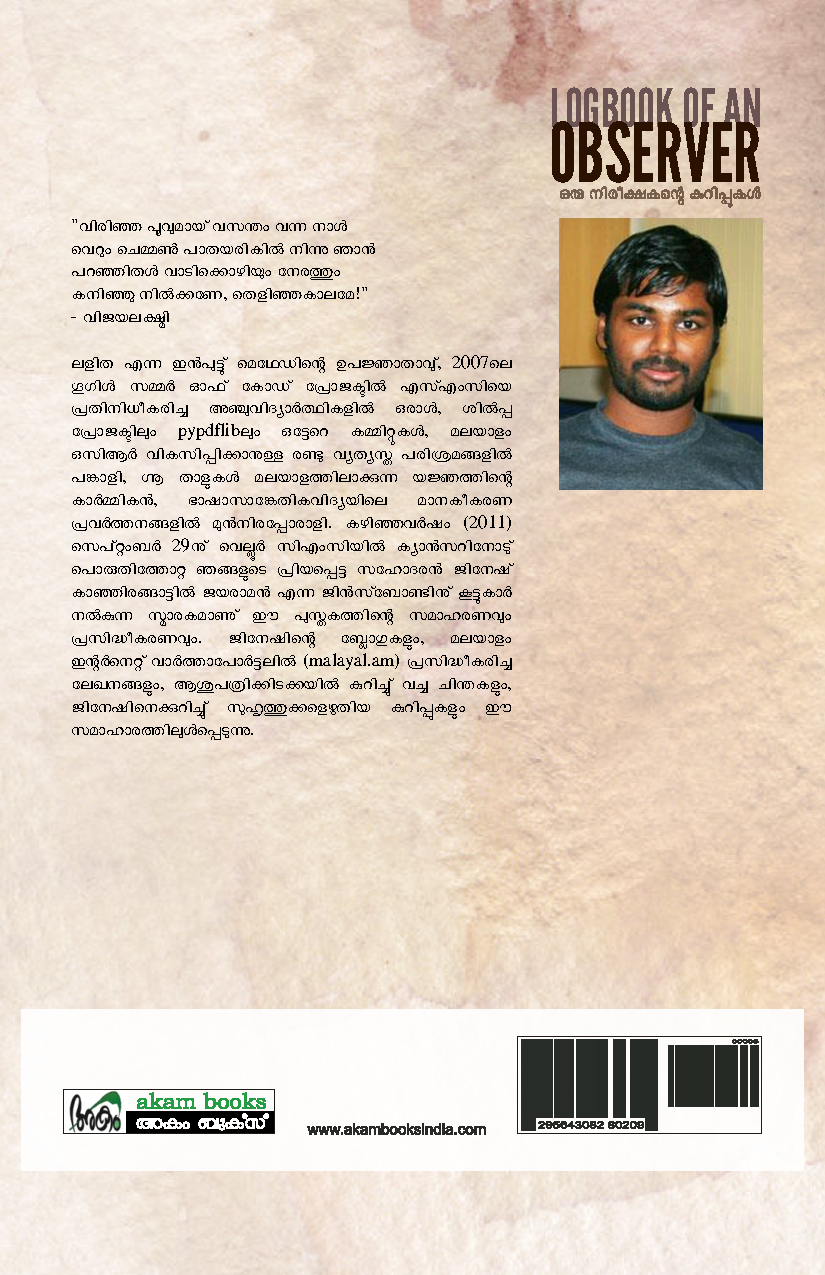
\includepdf{backcover}

%--------------------------------------------------------------------

\end{document}
